% preamble

\documentclass[11pt,oneside,reqno,xcolor=dvipsnames]{article} % font size: 12pt, one-sided pages, equation numbers on right side, availability of xcolors

\usepackage[USenglish]{babel} % language: USenglish, alternatives: UKenglish, ngerman
\usepackage[utf8]{inputenc} % input encoding: UTF8

\usepackage[a4paper,top=30mm,bottom=20mm,left=27.5mm,right=27.5mm]{geometry} % page structure, page size: DIN A4
\usepackage{lscape} % landscape format

\pdfminorversion=6 % create a PDF with version 1.6 (default=1.5)

\frenchspacing % not a larger space after end of sentence
%\setlength{\parindent}{0cm} % paragraph indentation (default = 1.5em for 12pt font size)
\usepackage{setspace} % space between lines
    \linespread{1.5} % linespacing: 1.5 lines; alternative: \onehalfspacing = \linespread{1.24}

\usepackage{amsmath} % mathematical features
\usepackage{mathtools} % mathematical tools for amsmath: numbering only for specific equations, extensible arrows, etc.
\usepackage{array} % extensions for array and tabular environments
    \setlength\arrayrulewidth{0.3pt} % thickness of lines in arrays/tabulars (default = 0.4pt)

\usepackage{tocloft} % control table of contents, list of tables, list of figures
\usepackage{titlesec} % additional features for (sub-)sections
    \titleformat*{\section}{\bfseries} % section: bold and normal font size
    \titleformat*{\subsection}{\bfseries} % subsection: bold and normal font size
    \titleformat*{\subsubsection}{\normalsize\bfseries} % subsection: bold and normal font size
    \titleformat*{\paragraph}{\normalsize\bfseries} % paragraph: bold and normal font size
    \titleformat{name=\section}{\normalfont\bfseries}{\thesection}{0.7em}{\hspace{0em}}{} % section: smaller horizontal space between toc number and caption
    \titleformat{name=\subsection}{\normalfont\bfseries}{\thesubsection}{0.7em}{\hspace{0em}}{} % subsection: smaller horizontal space between toc number and caption
    \titleformat{name=\subsubsection}{\normalfont\normalsize\bfseries}{\thesubsubsection}{0.7em}{\hspace{0em}}{} % subsubsection: smaller horizontal space between toc number and caption
    \titleformat{name=\paragraph}[runin]{\normalfont\normalsize\bfseries}{\theparagraph}{0.7em}{\hspace{0em}}{} % paragraph: smaller horizontal space between toc number and caption

\usepackage[hang,flushmargin,symbol]{footmisc} % footnotes, hang: hanging footnotes, flushmargin: no indentation, symbol: allow for symbols
    \renewcommand*{\thefootnote}{\fnsymbol{footnote}} % footnote symbols for title page (*, etc.)
    \newcommand\fnsep{\textsuperscript{,}} %command to separate subsequent footnotes with comma (note: "multiple" option for footmisc clashes with hyperref package)

\usepackage{lipsum} % insert blind text

\usepackage{amssymb} % additional symbols
\usepackage{marvosym} % additional symbols
\usepackage{ifsym} % additional symbols
\usepackage{wasysym} % additional symbols
\usepackage{eurosym} % additional symbols
\usepackage{textcomp} % additional symbols
\usepackage{MnSymbol} % additional symbols

\newcommand{\longeq}{\scalebox{1.25}[1]{=}} % "\longeq" yields long equal sign (==)


\usepackage{caption} % configure captions of figures/tables
\usepackage{subcaption} % captions for subfigures/subtables
\usepackage[capposition=top]{floatrow} % additional features for figures/tables, capposition=top: caption above table/figure
\usepackage{float} % improves the interface for defining floating objects such as tables/figures (load after floatrow package)
\usepackage{afterpage} % execute command after next break


\usepackage{xcolor} % additional colors
\usepackage{soulutf8} % underlining, striking out, highlighting, etc. (for UTF8 use)
    \DeclareRobustCommand{\hlcyan}[1]{{\sethlcolor{cyan}\hl{#1}}} % new command "\hlcyan" for comments in blue
    \DeclareRobustCommand{\hlviolet}[1]{{\sethlcolor{violet}\hl{#1}}} % new command "\hlviolet" for comments in violet

\usepackage{tabularx} % new features for tables
    \newcolumntype{L}[1]{>{\raggedright\arraybackslash}p{#1}} % flush-left alignment with manual width for table column
    \newcolumntype{C}[1]{>{\centering\arraybackslash}p{#1}} % centered alignment with manual width for table column
    \newcolumntype{R}[1]{>{\raggedleft\arraybackslash}p{#1}} % flush-right alignment with manual width for table column
\usepackage{multirow} % connect cells within tables
\usepackage{hhline} % double horizontal lines in array/tabular
\usepackage{rotating} % rotate text
\usepackage[flushleft]{threeparttable} % structured scheme for tables (caption, table, notes), flushleft: no hanging indentation on notes
\usepackage{diagbox} % slash-separated parts of a cell within table
\usepackage{colortbl} % colors in tables
\usepackage{arydshln} % dash lines in array/tabular (load after colortbl package)
    \setlength\dashlinegap{3pt} % amount of each gap between dash segments (default = 4pt)
\usepackage{booktabs}% extra commands for tables
    \newcommand{\tabitem}{~~\llap{--\!}~~} % define \tabitem command for bullets within tabular environment

\usepackage{pgfplots} % diagrams
    \pgfplotsset{compat=newest}
    \usepgfplotslibrary{statistics} % necessary for boxplots
    %\usepgfplotslibrary{external} % plot figures externally to increase memory of WinEdt, necessary: add "--shell-escape" to Options/Execution Modes/Console Applications/Accesoires/PDFtexifiy/Command Line/switches
    %\tikzexternalize % plot figures externally to increase memory of WinEdt, necessary: add "--shell-escape" to Options/Execution Modes/Console Applications/Accesoires/PDFtexifiy/Command Line/switches
    \usepgfplotslibrary{fillbetween} % shade areas
    \pgfkeys{/pgf/number format/.cd,1000 sep={}} % no 1000's separator (,) in diagrams
\usepackage{tikz} % drawings
    \usetikzlibrary{decorations.pathreplacing,decorations.markings, patterns, intersections} % decorations.pathreplacing: different line types, decorations.markings: new line types, patterns: fillings, intersection: coordinates relative to intersection

\usepackage{enumitem} % lists

\usepackage{graphicx} % include pictures, "\scalebox" command
\usepackage{pdfpages} % include PDFs

\usepackage{comment} % selectively exclude portions of text

\usepackage{bm} % bold math symbols


\usepackage[backend=bibtex,natbib=true,style=authoryear,doi=false,isbn=false,url=false,eprint=false,giveninits=true,uniquename=false,dashed=false,maxnames=2,maxbibnames=30]{biblatex} % bibliography, backend=bibtex: use bibtex instead of biber, natbib=true: use natbib, style=authoryear: set bibliography style, doi/isbn/url/eprint=false: suppress ISBN, DOI etc., giveninits=true: abbreviate first and middle names with initials, uniquenames=false: do not distinguish between authors with same surname and first name initial, dashed=false: suppress dash substitution for recurring author lists, maxnames=2: use "et al." for more than two authors, maxbibnames=30: maximum number of authors is 30

\addbibresource{arXiv} % include Jabref file with entries for bibliography (without ".bib" ending), notes: - name of bib file must not include empty spaces, - pages must be typed as "XXXX--XXXX", - put "Online First" in page item, write "1st/2nd/... Edition" in edition item for books

\usepackage{csquotes} % typesetting of quoted texts according to rules of specific language (recommended for BibLaTeX)



     % always lastname-firstname order (for authors and editors)
    \DeclareNameAlias{sortname}{family-given} %authors
    \DeclareNameAlias{default}{family-given} %editors



    % remove inverted commas for title
    \DeclareFieldFormat[article,inbook,incollection,inproceedings,patent,thesis,unpublished]{title}{#1\isdot}



    % remove "pp." for pages
    %\DeclareFieldFormat{pages}{#1}



    % article: no "In:" before journal title
    \renewbibmacro{in:}{\ifentrytype{article}{}{\printtext{\bibstring{in}\intitlepunct}}}



    % article: number of volume in parentheses
    \renewbibmacro*{volume+number+eid}{%
      \printfield{volume}%
    %  \setunit*{\adddot}% deleted
      \setunit*{\addnbthinspace}% small space inserted; for normal space use "\addnbspace"
      \printfield{number}%
      \setunit{\addcomma\space}%
      \printfield{eid}}
    \DeclareFieldFormat[article]{number}{\mkbibparens{#1}}



    % incollection: comma between incollection title and editors
    \usepackage{xpatch}
    \def\dopatchbibdrivereditorcomma#1{%
      \xpatchbibdriver{#1}
        {\usebibmacro{maintitle+booktitle}%
         \newunit\newblock}
        {\usebibmacro{maintitle+booktitle}%
         \setunit{\addcomma\space}\newblock}
        {}
        {\typeout{failed to patch driver for type #1}}}
    \forcsvlist{\dopatchbibdrivereditorcomma}{inbook,incollection,inproceedings}


    % incollection: comma between editors and location
    \renewbibmacro*{byeditor+others}{%
      \ifnameundef{editor}
        {}
        {\usebibmacro{byeditor+othersstrg}%
         \setunit{\addspace}%
         \printnames[byeditor]{editor}%
         \clearname{editor}%
         \addcomma}%
      \usebibmacro{byeditorx}%
      \usebibmacro{bytranslator+others}}


    % misc: no italics for title of discussion paper
    %\DeclareFieldFormat[misc]{title}{#1}

    % correct hyperlink for "References" Section
    \makeatletter
    \pretocmd{\blx@head@bibintoc}{\phantomsection}{}{\ddt}
    \makeatother

    \AtBeginBibliography{
    	%\renewcommand*{\mkbibnamefamily}[1]{\textsc{#1}} %capitalization of authors
    	\renewcommand*{\mkbibnameprefix}[1]{\textsc{#1}} %
    }



    % do not separate author and year in in-text citations with a comma
    %\renewcommand*{\nameyeardelim}{\space}





    % add hyperlink for command "citeyearpar"
    \DeclareCiteCommand{\citeyear}
        {}
        {\bibhyperref{\printdate}}
        {\multicitedelim}
        {}
    \DeclareCiteCommand{\citeyearpar}
        {}
        {\mkbibparens{\bibhyperref{\printdate}}}
        {\multicitedelim}
        {}






\usepackage[colorlinks=true,linkcolor=blue,citecolor=blue,urlcolor=black,linkbordercolor=cyan,citebordercolor=cyan,urlbordercolor=cyan,hyperfootnotes=true]{hyperref} % cross-referencing, colorlinks: emphasize words instead of using boxes, color: blue coloring, bordercolor: cyan boxes, hyperfootnotes: emphasize also footnotes (always load as last package)



% customize boxplots
\pgfplotsset{
boxplot/every average/.style={solid,/tikz/mark=square}, % disable dashs, square as sybol for average
boxplot/every box/.style={solid}, % disable dashs
boxplot/every whisker/.style={solid}, % disable dashs
boxplot/every median/.style={solid}, % disable dashs
}

% define legend image for error bar plot --> add "error bar plot" to "\addplot(...)" command
\pgfplotsset{error bar legend/.style={%
    /pgfplots/legend image code/.prefix code={%
      \pgfkeysgetvalue{/pgfplots/error bars/error mark}{\pgfplotserrorbarsmark}%
      \draw[%
        /pgfplots/every error bar,
        mark=\pgfplotserrorbarsmark,
        /pgfplots/error bars/error mark options,
        sharp plot,
        ##1
      ] plot coordinates {(0.3cm, -0.15cm) (0.3cm, 0.15cm)};%
      %\pgfkeysalso{%
        %/pgfplots/error bars/draw error bar={(0.3cm, 0cm)}{(0.3cm, 0.15cm)},
        %/pgfplots/error bars/draw error bar={(0.3cm, 0cm)}{(0.3cm, -0.15cm)},
      %};
    }
  }
}














\begin{document}



\begin{titlepage}
\begin{center}

%\vspace*{0.1cm}

\Large

\textbf{Minimum Wages in Concentrated Labor Markets}

\normalsize

\vspace*{1.75cm}

%one author
\href{http://www.iab.de/en/ueberblick/mitarbeiter.aspx/Mitarbeiter/12380200}{\textcolor{black}{\textbf{Martin Popp}}} \\
\href{http://www.iab.de/en/iab-aktuell.aspx}{\textcolor{black}{IAB}} \textcolor{black}{\&} \href{https://www.fau.eu/}{\textcolor{black}{University of Erlangen-Nuremberg}} \\[-0.2cm]
\textcolor{black}{martin.popp@iab.de}

\vspace*{0.9cm}



arXiv Discussion Paper\footnote[1]{\textbf{Corresponding Address:} Martin Popp, Institute for Employment Research (IAB), Regensburger Straße 100, 90478 Nuremberg, Germany. Email: martin.popp@gmx.net, Phone: $\plus$49 (0)911/179-3697. \newline \textbf{Acknowledgments:} I am grateful to the Joint Graduate Program of IAB and FAU Erlangen-Nuremberg (GradAB) for financial support of my research. I thank Miren Azkarate-Askasua, Lutz Bellmann, Mario Bossler, David Card, Matthias Collischon, Martin Friedrich, Nicole Gürtzgen, Anna Herget, Katrin Hohmeyer, Etienne Lal\'{e}, Ioana Marinescu, Andreas Peichl, Michael Oberfichtner, and Duncan Roth for helpful discussions and suggestions. Earlier versions of this paper were presented at the 12th Ph.D.\ Workshop ``Perspectives on (Un-)Employment'' in Nuremberg (IAB), the 4th Workshop on Labor Statistics in virtual format (IZA), the 26th SOLE Conference in virtual format (U Philadelphia), the 25th Spring Meeting of Young Economists in virtual format (U Bologna) as well as in seminars in Nuremberg (IAB/FAU) and Uppsala (IFAU).}  \\
23 November, 2021 %\today
%\\ (Please do not cite or circulate without permission.)
\\[1.5cm]

\begin{abstract} %100-150 words
\onehalfspacing
\noindent Economists increasingly refer to monopsony power to reconcile the absence of negative employment effects of minimum wages with theory. However, systematic evidence for the monopsony argument is scarce. In this paper, I perform a comprehensive test of monopsony theory by using labor market concentration as a proxy for monopsony power. Labor market concentration turns out substantial in Germany. Absent wage floors, a 10 percent increase in labor market concentration makes firms reduce wages by 0.5 percent and employment by 1.6 percent, reflecting monopsonistic exploitation. In line with perfect competition, sectoral minimum wages lead to negative employment effects in slightly concentrated labor markets. This effect weakens with increasing concentration and, ultimately, becomes positive in highly concentrated or monopsonistic markets. Overall, the results lend empirical support to the monopsony argument, implying that conventional minimum wage effects on employment conceal heterogeneity across market forms. % 141 words
\end{abstract}




\vspace*{1cm}
\end{center}
\small

\textbf{JEL Classification:}\,  % decreasing order of relevance
J42, J38, D41, J23 \\[0.5cm]

\textbf{Keywords:}\,  % decreasing order of relevance
minimum wage, labor market concentration, monopsony, labor demand





\end{titlepage}





%\tableofcontents

%switch to arabic numbers for footnotes
\renewcommand*{\thefootnote}{\arabic{footnote}}
\setcounter{footnote}{0}


\newpage

\normalsize



% main body

\section{Introduction}
\label{sec:1}



%motivation
Although minimum wage regulations are in effect in many economies, the benefits and costs of such an intervention remain a controversial topic. For instance, there is an ongoing debate in the U.S.\ about raising the federal minimum wage from \$7.25 to \$15. While proponents of minimum wages seek to raise the pay of low-wage workers, opponents warn that this policy harms employment. Building on the notion of competitive labor markets, economists have long argued that firms respond to higher minimum wages with a reduction in employment. In contrast, the empirical minimum wage literature shows inconclusive results: whereas some studies find negative employment effects (e.g., Neumark/Wascher, \citeyear{NeumarkWascher1992}; Currie/Fallick, \citeyear{CurrieFallick1996}; Clemens/Wither, \citeyear{ClemensWither2019}; Bossler/Gerner, \citeyear{BosslerGerner2020}), a plethora of articles is not in line with conventional wisdom and reports employment effects of minimum wages to be close to zero (e.g., Card/Krueger, \citeyear{CardKrueger1994}; \citealp{DubeEtAl2010}; \citealp{AllegrettoEtAl2011}; \citealp{CengizEtAl2019}; Harasztosi/Lindner, \citeyear{HarasztosiLindner2019}; \citealp{DustmannEtAl2021}).\footnote{For reviews on the international minimum wage literature, see \citet{BrownEtAl1982}, \citet{CardKrueger1995}, \citet{DoladoEtAl1996}, \citet{Brown1999}, \citet{NeumarkWascher2008}, \citet{DoucouliagosStanley2009}, \citet{BelmanWolfson2014}, \citet{Neumark2019}, \citet{WolfsonBelman2019}, or \citet{NeumarkShirley2021}. \citet{Moeller2012} as well as \citet{FitzenbergerDoerr2016} provide overviews on eight studies evaluating the impact of sectoral minimum wages in Germany. In addition, \citet{CaliendoEtAl2019} review the literature on the introduction of the 2015 nation-wide minimum wage in Germany.} Many of these studies refer to firms' monopsony power to reconcile the absence of negative employment effects of minimum wages with theory. When employees are unlikely to transition to competitors, monopsony power enables firms to push workers' wages below marginal productivity. In such a setting, an adequate minimum wage can counteract monopsonistic exploitation without having adverse consequences on employment. However, systematic empirical support for the monopsony argument is scarce.


%this paper
In this paper, I calculate measures of labor market concentration to perform a direct and comprehensive empirical test of monopsony theory. Labor market concentration gives rise to monopsony power for two reasons: First, individuals in highly concentrated labor markets face only a limited range of potential employers. As a direct consequence, these workers will adjust their labor supply to the single firm less sensitively to wages. Second, labor market concentration facilitates anti-competitive collusion between firms which further restricts personnel turnover. I make use of both channels and produce fine-grained measures of labor market concentration to gauge the degree of firms' monopsony power in the labor market. To this end, I leverage administrative records on the near-universe of workers' employment spells in the German labor market between 1999 and 2017.

The test of monopsony theory refers to sixteen low-wage sectors in Germany for which the Ministry of Labor and Social Affairs has declared sector-specific minimum wages. Prior to minimum wage legislation in these sectors, I examine whether, in line with monopsony theory, firms in concentrated labor markets exert their monopsony power by lowering both wage rates and employment in the absence of wage floors. As this hypothesis is supported by the data, I scrutinize next whether minimum wages can counteract monopsonistic exploitation without harming employment, the so-called ``monopsony argument''. Given a significant bite of these sectoral wage floors, the analysis allows to endorse the monopsony argument under two conditions: On the one hand, slightly concentrated or competitive labor markets must experience negative minimum wage effects on employment. On the other hand, this negative effect must weaken for increasing levels of labor market concentration. Moreover, provided that minimum wages are set close to equilibrium rates, minimum wage effects on employment can even turn out positive in highly concentrated or monopsonistic markets.

%results: labor market concentration
The full coverage of workers and establishments in the German social security data allows me to calculate unbiased measures of concentration of employees on employers, the classical source of monopsony power, for each local labor market in Germany between 1999 and 2017. In this study, I follow common practice and define labor markets as pairs of industries and commuting zones. For the baseline delineation with 4-digit industries, I document high concentration in 51.8 percent of all labor markets and for 12.9 percent of workers, operationalized by a market-level Herfindahl-Hirschman Index (HHI) above 0.2 from E.U.\ antitrust policy. At the same time, the HHI indices show considerable heterogeneity across industries and commuting zones. Nonetheless, with a mean HHI of around 0.35, labor market concentration in Germany has on average remained relatively stable throughout the last two decades. Overall, the high levels of labor market concentration indicate substantial monopsony power in German labor markets. This result is consistent with dynamic monopsony models on Germany which estimate the labor supply curve to the firm to be rather inelastic.


%results: effects of LM concentration
Building on the concentration indices, I document that firms indeed lowered both wages and employment in concentrated labor markets -- as put forward by monopsony theory. Specifically, I select all those observations of firms in the respective minimum wage sectors before wage floors came into force. For these observations, I perform OLS and instrumental variables (IV) regressions of firms' wages and employment on market-level HHI values, based on yearly panel information covering 1999 to 2014. For the IV estimations, I construct a so-called ``leave-one-out'' instrument for HHI as the average of the log inverse number of firms in the same industry for all other commuting zones. Importantly, this instrument harnesses variation from national changes in labor market concentration over time and, thus, rules out potentially endogenous variation in HHI that originates from the very same labor market. Although OLS and IV findings are qualitatively alike, the IV estimates turn out to be larger in absolute terms. The baseline IV specifications indicate that a 10 percent increase in labor market concentration reduces mean wages in a firm by 0.5 percent and firm-level employment by 1.6 percent, thus lending support to monopsonistic exploitation in concentrated labor markets. The results are robust to alternative labor market definitions or concentration measures and apply for different subgroups of workers. Moreover, monopsonistic exploitation turns out to be particularly salient at the upper end of the wage distribution and in labor markets with low outward mobility.


%results: minimum wage effects
Next, I analyze whether minimum wages represent an effective policy to counteract monopsonistic exploitation. Specifically, I explore whether firms' responses to minimum wages vary by market structure. To this end, I regress firm-level wages and employment on minimum wages and an interaction term with labor market concentration that serves to inspect the moderating role of monopsony power. Before turning to employment effects, I verify whether sectoral minimum wages in Germany effectively increased the pay of the workforce. I find that a 10 percent increase in sectoral minimum wages leads, on average, to a 0.7 percent increase of earnings in perfectly competitive markets (with zero HHI) where wages are expected to follow marginal productivity. In line with theory and the evidence on monopsonistic exploitation, this positive wage effect becomes more pronounced with increasing levels of labor market concentration under which workers' wages are pushed below marginal productivity. Eventually, in the polar case of a monopsony (HHI equals one), a 10 percent minimum wage increase is associated with a rise in mean earnings by 3.3 percent.

%Vice versa, the estimation sample is now restricted to all firm observations that must obey a sectoral minimum wage.

Given this bite, I arrive at a negative minimum wage elasticity of employment around -0.3 for markets with zero HHI, thus corroborating the notion that minimum wages lower employment in competitive environments. However, in line with the rationale of the monopsony argument, I report near-zero effects in moderately concentrated and significantly positive elasticity around 0.9 in highly concentrated labor markets. Following theory, the minimum wage effect on employment is non-linear in highly concentrated labor markets: at first, the positive effect on firms' employment increases with the underlying bite but falls rapidly when the minimum wage is set close to the median wage of the firm. In general, the results are not sensitive to including alternative interaction effects, concentration indices as well as labor market definitions and hold for a large number of subgroups. Moreover, additional checks can rule out an omitted variable bias from interactions with product market concentration or firm productivity, thus endorsing labor market concentration as the true moderator of minimum wage effects. Although no theoretical structure is imposed upon the regressions, the joint pattern of wage and employment elasticities provides systematic evidence for the monopsony argument. Hence, when reasonably set and rigorously enforced, minimum wages constitute an effective measure to counteract monopsonistic exploitation without detrimental or, in extreme cases of labor market concentration, even positive effects on employment.


In a last step, I combine estimated minimum wage elasticities of earnings and employment to identify the underlying own-wage elasticity of labor demand along the distribution of labor market concentration. As the HHI increases, significantly negative elasticities for low HHI values contrast with significantly positive elasticities in high-HHI environments. Given this pattern, a comparison with prior estimates from the German minimum wage literature suggests that the frequent finding of near-zero employment effects stems in part from pooling heterogeneous effects for different levels of labor market concentration.

%related literature & research gaps
This paper contributes to the understanding of monopsonistic labor markets and minimum wage effects in several ways. First, I provide first evidence on labor market concentration in Germany. The concentration of workers on employers constitutes a key source for monopsony power that employers may exert over their employees. In his pioneering work, \citet{Bunting1962} was the first to calculate measures of labor market concentration for U.S.\ local labor markets. In recent years, the literature on labor market concentration experienced a sudden revival \citep{AzarEtAl2017} spurred by the recognition of a falling labor share in the U.S. \citep{AutorEtAl2020}.\footnote{In the appendix, I review the empirical literature on labor market concentration (see Table \ref{tab:C1}).} The concentration indices from this study mirror international evidence which is unanimous that labor market concentration is substantial. \citet{AzarEtAl2020} harness data on U.S.\ online job vacancies and conclude that 60 percent of labor markets are highly concentrated. For France, \citet{MarinescuEtAl2021} report an average labor-market HHI of 0.2 for new hires. \citet{Martins2018} arrives at a mean HHI of 0.4 for employment in Portuguese labor markets. However, evidence on the development of labor market concentration over time is more mixed. Stable concentration in Germany contrasts with contemporaneous evidence from the U.S., where local labor markets became less concentrated \citep{Rinz2020}, and the U.K., which featured a bell-shaped path in labor market concentration \citep{AbelEtAl2018}.




Second, this study entails an overall and direct empirical test of monopsony theory. \citet{Robinson1933} established the theory of a single profit-maximizing employer who cuts employment along a positively sloped labor supply curve to the firm to suppress workers' wages. \citet{Manning2003a} popularized the estimation of dynamic monopsony models to quantify the degree of monopsony power in the labor market. These semi-structural models commonly estimate rather inelastic labor supply elasticities to the single firm, indicating a high level of wage-setting power of firms (Sokolova/Sorensen, \citeyear{SokolovaSorensen2021}). Similar results are obtained by another strand of the literature that regresses firm-specific employment on plausibly exogenous variation in wage rates (e.g., \citealp{Falch2010}; \citealp{StaigerEtAl2010}). Surprisingly, direct empirical evidence whether firms in fact exercise their monopsony power to push down wages was hardly available until recently. \citet{Webber2015} finds that firms pay lower wages when the wage elasticity of labor supply is less elastic. Meanwhile, the growing literature on labor market concentration delivers numerous estimates with a negative impact of HHI on earnings (\citealp{AbelEtAl2018}; \citealp{AzarEtAl2017}; \citealp{BassaniniEtAl2019}; \citealp{BenmelechEtAl2020}; \citealp{DodiniEtAl2020}; \citealp{Lipsius2018}; \citealp{Martins2018}; Prager/Schmitt, \citeyear{PragerSchmitt2021}; Qiu/Sojourner, \citeyear{QiuSojourner2019}; \citealp{Rinz2020}; \citealp{SchubertEtAl2020}; \citealp{Thoresson2021}). \citet{MarinescuEtAl2021} find that an increase in labor market concentration comes along with less hires. By contrast, and building on firm-level data, this study is the first to simultaneously show that firms in concentrated markets not only suppress wages but that they also do so by reducing their employment -- the key rationale of monopsony theory.

Third, my results provide systematic empirical support for the monopsony argument: whereas minimum wage effects are detrimental to employment in competitive labor markets, they do not impact or even stimulate employment in concentrated labor markets. Studies from both the international and the German minimum wage literature frequently arrive at near-zero employment effects (Card/Krueger \citeyear{CardKrueger1995}; Neumark/Wascher \citeyear{NeumarkWascher2008}; \citealp{Moeller2012}; \citealp{CaliendoEtAl2019}). Many of these articles use the notion of oligopsonistic or monopsonistic market structures to reconcile the absence of considerable job destruction with economic theory (e.g., Card/Krueger \citeyear{CardKrueger1994}; \citealp{DustmannEtAl2021}). Nevertheless, direct empirical evidence in favor of the monopsony argument is scarce \citep{Neumark2019}.\footnote{\citet{BloemerEtAl2018} structurally estimate an equilibrium job search model for the German labor market and simulate minimum wage effects by search frictions.} An exception is the study from \citet{AzarEtAl2019a} that examines the role of labor market concentration for the minimum wage elasticity of employment in three occupations from the U.S.\ general merchandise sector. In a similar fashion, \citet{Munguia2020} focuses on minimum wage effects for U.S.\ teenage employment. At the market level, both studies find that negative employment effects of minimum wages diminish with increasing labor market concentration. In contrast to both studies, however, I do not analyze variation in aggregate employment per labor market but instead make use of micro-level information on firms, that is, the unit where personnel decisions take place. Hence, the firm-level perspective allows to differentiate sustained employment relationships from dismissed workers who took up a job with another firm in the same labor market. Moreover, the support of the monopsony argument in this study is not limited to a narrow set of workers. Rather, it extends to overall employment across the universe of establishments from sixteen heterogeneous low-wage sectors.





Fourth, under specific conditions, the German Federal Ministry of Labor and Social Affairs has the right to declare collectively agreed wages to be universally binding. Since 1997, such minimum wages have come into effect in an increasing number of sectors, with exact levels being modified with the cycle of collective bargaining. As of 2015, more than 12 percent of all workers in Germany were employed in these minimum wages sectors. Several studies have investigated the effects of these minimum wages on single targeted sectors, such as main construction (König/Möller, \citeyear{KoenigMoeller2009}), waste removal \citep{EgelnEtAl2011}, or nursing care \citep{BoockmannEtAl2011c}. To date, however, an overall quantitative analysis is missing. This study is the first to complement the literature with an analysis across sectors, thus providing holistic evidence on the labor market effects of sectoral minimum wages in Germany.


%organization paragraph
The remainder of the paper has the following structure: Section \ref{sec:2} establishes the monopsony theory and its role for earnings, employment, and minimum wage effects. Section \ref{sec:3} outlines the institutional setting of sectoral minimum wages in Germany. Section \ref{sec:4} describes the administrative data. In Section \ref{sec:5}, I provide descriptive evidence on labor market concentration in Germany. Section \ref{sec:6} seeks to estimate the causal effect of labor market concentration on earnings and employment absent any minimum wage regulations. In Section \ref{sec:7}, I investigate whether minimum wage effects vary by market form. The discussion in Section \ref{sec:8} elaborates on whether monopsony power in the labor market can rationalize the widespread finding of near-zero minimum wage effects on employment. I conclude in Section \ref{sec:9}.












\section{Theoretical Background}
\label{sec:2}


A brief review on the role of minimum wages by market form helps to clarify the hypotheses to be tested in the empirical part of this paper. The theory of perfect competition constitutes the standard framework for analyzing minimum wage effects (see Figure \ref{fig:A1}). In this setting, a large number of atomistic firms face an infinitely elastic labor supply (LS) curve that implies constant marginal cost of labor (MCL) at market wage $w^{C}$. In equilibrium, each profit-maximizing firm optimizes employment $L$ such that the marginal revenue product of labor (MRPL) equals the wage rate. In default of other channels of adjustment, the introduction or rise of a binding minimum wage $w^{min}$ raises marginal cost and, thus, makes firms lay off the least productive units of labor. As a result, minimum wages initiate unambiguously negative effects on employment along the intensive and/or the extensive margin \citep{Stigler1946}.\footnote{The negative employment effects may materialize in terms of substitution effects (more use of other input factors) and/or scale effects (lower output). Further, the overall minimum wage effect on employment does not only capture adjustment within surviving firms but also separations on account of firm closures.}


During the early 1990s, however, novel research designs delivered near-zero employment effects (\citealp{Card1992a}; \citealp{Card1992b}; Card/Krueger, \citeyear{CardKrueger1994}) and, thus, challenged the common belief among economists that minimum wages are detrimental to employment \citep{BrownEtAl1982}. The minimum wage literature offers several explanations to reconcile the absence of disemployment effects with the neoclassical paradigm of competitive labor markets \citep{Schmitt2015}. Indeed, any specification in terms of heads (instead of hours) will underestimate the disemployment effect to the extent that minimum wage responses occur along the intensive margin. In addition, firms can pass on the higher wage costs to customers in the form of price increases \citep{Lemos2008}. Moreover, with inadequate enforcement, studies will report small employment effects simply because firms did not fully comply with the minimum wage regulation (Ashenfelter/Smith, \citeyear{AshenfelterSmith1979}). Institutions, such as worker unions or work councils, may further alleviate employment responses (through a smaller bite or objections to scheduled dismissals, respectively). Moreover, in an efficiency wage model, minimum wages carry the advantage that they enhance workers' productivity (Rebitzer/Taylor, \citeyear{RebitzerTaylor1995}).

Importantly, monopsony theory -- the argument most frequently put forward to rationalize the absence of negative minimum wage effects -- departs from perfect competition (Card/Krueger, \citeyear{CardKrueger1995}). The textbook monopsony model from \citet{Robinson1933} postulates a single firm that is the only buyer in the labor market (see Figure \ref{fig:A1}). Such a profit-maximizing monopsonist equates MRPL with MCL to choose the optimal wage-employment combination on the labor supply curve to the firm. The firm derives its monopsony power from the fact that the wage elasticity of labor supply to the firm $\mu$ is less than perfectly elastic, that is, an infinitesimally small wage cut does not make all workers leave the firm. In case the firm pays all workers the same wage rate, such an upward-sloping LS curve gives rise to increasing marginal cost of labor.\footnote{\citet{Robinson1933} also refers to the possibility that firms treat each worker differently. Under first-order wage discrimination, the monopsonist pays workers their individual reservation wage. In such a case, the monopsonist will realize the competitive level of employment while skimming all of workers' rents.} Unlike in the competitive model, the monopsonist cannot recruit workers at the ongoing wage rate but, instead, must offer higher wages both to new hires and incumbent workers. Consequently, the firm will find it optimally to lower the wage rate $w^{M}$ by constraining employment $L^{M}$ below the competitive level $L^{C}$. As a result, workers earn less than their marginal productivity with a markdown equal to the reciprocal of the wage elasticity of labor supply to the firm: $ \frac{MRPL-w}{w} = \mu^{-1} $ \citep{AshenfelterEtAl2010}.   %Thus, under monopsony, both wages and employment fall short of their equilibrium levels from perfect competitive.



In monopsonistic labor markets, a minimum wage entails less negative employment effects than under perfect competition and, for moderately-set wage floors, can even stimulate employment (Stigler, \citeyear{Stigler1946}; Lester, \citeyear{Lester1947}). Specifically, the employment effect differs between three regimes: First, in the unconstrained regime below $w^{M}$, minimum wages do not bind. Second, in the supply-determined regime, the minimum wage lies in the interval between the $w^{M}$ and the $w^{C}$. Crucially, such a regulation renders marginal cost of labor constant because hiring at the minimum wage no longer involves higher wages for incumbents (who also earn the minimum wage). The reduced marginal cost will make the monopsonist increase employment until the minimum wage meets the labor supply curve (after which MCL coincides with pre-minimum-wage levels). Hence, the minimum wage eliminates the firm's incentive to exploit inelastic labor supply at the bottom part of the wage distribution. \citet{Manning2011} shows that, along the supply-determined regime, a lower value for $\mu$ is associated with more positive minimum wage effects on wages and employment. Third, in the demand-determined regime, the minimum wage exceeds $w^{C}$ and the minimum wage materializes along the negatively sloped labor demand curve. Thus, initial job creation from the supply-determined regime may be (partly) offset.\footnote{If the minimum wage is set beyond the marginal revenue product of labor absent the minimum wage, the overall minimum wage effect on employment will become negative. Hence, under monopsony, there is a non-monotonous relationship between minimum wages and overall employment effects.}



The case of a few employers in the labor market, a so-called oligopsony, constitutes a more general market structure in the midst of the two extreme settings described above. The Cournot oligopsony assumes $J$ firms to compete in factor quantities and nests perfectly competitive and monopsonistic labor markets as limiting cases (Boal/Ransom, \citeyear{BoalRansom1997}). Figure \ref{fig:A2} illustrates stylized minimum wage effects by market structure within a Cournot oligopsony of symmetric firms. With an increasing number of oligopsonists in the market, both the wage rate and employment converge towards competitive levels. Although the range of the supply-determined regime becomes increasingly smaller for higher $J$, an adequately-set minimum wage still results in overall job growth.\footnote{The symmetry assumption implies that changes in firm-specific and overall employment exhibit identical signs. In the asymmetric case, the overall effect remains the same but underlying firm-level employment may either increase or decrease depending on the firms' MRPL curves \citep{Manning2003a}.}\fnsep\footnote{The supply-determined regime disappears in the polar case of perfect competition. With $N$ or $\mu$ converging to infinity, no monopsonistic exploitation will take place. In such a setting, minimum wages are either non-binding or reduce employment along the labor demand curve.} Importantly, such a positive employment effect also holds for more elaborate models of monopsonistic competition (Bhaskar/To, \citeyear{BhaskarTo1999}; \citealp{Walsh2003}).\footnote{The model from \citet{BhaskarTo1999} explicitly accounts for firm entry and exit. In their setting, heterogeneous workers incur commuting cost to firms that are uniformly spaced around a unit circle of job characteristics. Building on their model, \citet{Walsh2003} shows that firm exits are not large enough to counterbalance the job growth in firms remaining in the market.} Thus, on average, minimum wages will cause more positive effects on firms' wages and less negative effects on firms' employment to the extent that the labor market is monopsonistic \citep{BhaskarEtAl2002}. In the following, I will use concentration indices to directly test these hypotheses based on variation in sectoral minimum wages from Germany.











\section{Institutional Framework}
\label{sec:3}

For many decades, high coverage rates of collective agreements ensured effective wage floors in Germany, stifling any discussion about the introduction of a nation-wide minimum wage \citep{BachmannEtAl2014}. But, in the last 25 years, Germany experienced a sharp decline in collective bargaining and rising inequality at the bottom of the wage distribution \citep{DustmannEtAl2009}. Against this backdrop, Germany became one of the last E.U.\ countries to impose a nation-wide minimum wage in 2015. Beginning in 1997, however, minimum wages had already come into force in a large variety of sectors.\footnote{Throughout this study, I distinguish between the concepts of ``sector'' and ``industry''. I define an ``industry'' as an entry within the German Classification of Economic Activities. On the contrary, I use the term ``sector'' to describe a (sub-)set of industries that share the same collective bargaining agreement and, consequently, the same minimum wage regulation.} These sectoral minimum wages were not set by government but, instead, originated from sector-wise collective bargaining agreements (CBA) that the Federal Ministry of Labor and Social Affairs (BMAS) declared universally binding. Over the years, sectoral minimum wages were subject to periodic adjustments, thus offering rich variation to study the minimum wage effects by market form.

Three independent pieces of legislation lay down the requirements of imposing sectoral minimum wages in Germany (see Table \ref{tab:B1} for an overview on minimum wage legislation in Germany). Since 1949, the Collective Bargaining Law (TVG) stipulates the general conditions for universal bindingness of CBAs. At request of either the worker union or the employer association, the BMAS, under certain conditions, may declare a CBA to be universally binding. The conditions are quite restrictive: an implementation necessitates consent from the umbrella organization of employers and, for many years, also required the coverage rate of firms subject to the CBA to exceed 50 percent.\footnote{In fact, a Bargaining Committee must give its approval to the declaration of universal bindingness by the BMAS. The Bargaining Committee has equal representation and consists of six members, three of whom are appointed from each of the national umbrella organizations of employees and employers.} Hence, minimum wages based on TVG could attain long-term relevance for few sectors, such as electrical trade.

Second, in 1996, the German parliament adopted the Posting of Workers Law (AEntG) to curtail wage competition in the construction sector \citep{Eichhorst2005}. Accordingly, foreign workers who are posted to German construction sites from abroad are subject to the same minimum working conditions of collective agreements that have been declared generally binding. When the AEntG was created, however, universal bindingness of a CBA could only be achieved under the restrictive conditions of TVG. Therefore, in 1998, the AEntG was amended to grant the BMAS the right to autonomously declare CBAs universally binding provided that there is a request from either of the two social partners. Subsequently, minimum wages based on AEntG came into effect for the sectors of main construction, roofing as well as painting and varnishing. Advocates of minimum wages recognized that the AEntG opened up a legal possibility to enforce minimum working conditions without explicit consent from employers. In the following years, the scope of the law steadily expanded to include other non-construction sectors where protection against foreign competition played only a subordinate role.\footnote{In 2009, the AEntG was modified such that the social partners must submit a joint request to the BMAS.} Eventually, the ambit of AEntG was opened to all sectors in 2014.

Third, the Temporary Work Law (AÜG) was revised in 2011 to prevent misuse of temporary work. Among other modifications, the reform permitted the imposition of a minimum wage for temporary workers. For this purpose, the social partners have to file a joint request of declaration of universal bindingness for their CBA. The BMAS can approve such a request in case the decree serves to ensure the financial stability of the social security system. With short interruptions, minimum wages apply in the temporary work sector since 2012.

A declaration of universal bindingness extends the coverage of minimum working conditions from a sector-specific CBA to the entire sector. Crucially, sectoral minimum wages apply to all firms in the sector, including those firms that decided against a membership in the employer association.\footnote{Legally, a firm belongs to a certain sector if it predominantly engages in this sector (i.e., with at least 50 percent of its business activity).} In principle, the regulation covers all employees in these firms, irrespective of their occupation or union membership. However, several sectors grant exemptions to white-collar workers or apprentices. Sectoral minimum wages expire with the end of the underlying CBA. Hence, transitional periods without a minimum wage regulation can occur until the BMAS declares a follow-up CBA universally binding. Since 2015, the wage floor falls back to the level of the nation-wide minimum wage in such cases.\footnote{The introduction of a nation-wide minimum wage in 2015 had also direct impact on sectoral minimum wages. First, the Minimum Wage Law (MiLoG) contains a three-year exemption for sectors that abide by minimum wages from AEntG or AÜG. However, this rule of transition encouraged several sectors to impose minimum wages that undercut the statutory minimum wage of 8.50 Euro per hour, namely hairdressing, slaughtering and meat processing, textile and clothing as well as agriculture, forestry and gardening. Second, the statutory minimum wage rendered sectoral wage floors useless in sectors where there was no consensus for a higher wage floor, such as industrial laundries or waste removal.}


To date, twenty sectors have imposed minimum wages throughout Germany.\footnote{In this study, I focus on those sectors that feature universally binding minimum wages throughout all federal states of Germany. Hence, sectors with wage floors for only local entities are not part of the analysis.} Table \ref{tab:B2} reviews sixteen of these sectors that allow for an identification in the German version of the NACE industry classification.\footnote{Specifically, I make use of the 1993, 2003 and 2008 versions of the 5-digit German Classification of Economic Activities (WZ) to determine the sector affiliation of establishments for the years 1999-2002, 2003-2007 and 2008-2017. The WZ Classification derives its four leading digits from the Statistical Classification of Economic Activities in the European Community (NACE). Unfortunately, the 5-digit WZ Classification is not sufficiently granular to identify establishments from the following minimum wage sectors: industrial laundries, specialized hard coal mining, public training services as well as money and value services.} In 2015, these sectors covered about 380,000 establishments and 5.2 million workers, representing 12.2 percent of overall employment in Germany. Sectoral values for the Kaitz Index suggest that the minimum wages bite strongly into the wage distribution. Interestingly, the Kaitz Index generally proves to be higher in East Germany despite the fact that, in many sectors, the social partners negotiated lower minimum wages compared to West Germany. The BMAS is obliged to publish sectoral minimum wages in the German Federal Bulletin (Bundesanzeiger) from which I extract sector-specific variation over the years 1999 to 2017 (see Figure \ref{fig:B1}).\footnote{Some sectors differentiate minimum wages by skill or task. In such cases, I select the lowest wage floor.}

Using differences-in-differences estimators, several articles investigate the effects of sectoral minimum wages on earnings and employment for specific sectors. For the main construction sector, \citet{KoenigMoeller2009} report the earnings effect to be more positive for individuals in East Germany than in West Germany. The authors find negative effects on the probability of remaining employed in East Germany whereas the results for West Germany are not significantly different from zero. Given a similar bite but more aggregate levels of observations, \citet{Rattenhuber2014} as well as vom Berge and Frings \citeyearpar{vomBergeFrings2020} report insignificant employment effects for both the West and the East German construction sector. \citet{BoockmannEtAl2013} use the introduction, abolishment and subsequent re-introduction of minimum wages in the electrical trade sector as natural experiments and detect no evidence for employment effects. \citet{Frings2013} finds employment effects neither for electrical trade nor painting and varnishing. The analysis from \citet{AretzEtAl2013} indicates that employment fell in East German roofing sector where the minimum wages bit particularly hard.

\citet{Moeller2012} as well as \citet{FitzenbergerDoerr2016} critically reflect on eight evaluation reports that investigate minimum wage effects for single sectors. Both reviews conclude that negative minimum wage effects on employment are rare and generally lower than expected. Möller (\citeyear{Moeller2012}, p.\ 339) reasons that ``[...] from a pure neoclassical point of view the findings are clearly at odds with expectations, but roughly in line with the view that there are important imperfections in the labor market.'' In this respect, \citet{Fitzenberger2009} proposes the use of friction parameters to empirically measure the degree of monopsonistic competition. In the following, I use indicators of labor market concentration to test the monopsony argument.








\section{Data}
\label{sec:4}

Calculating unbiased measures of labor market concentration necessitates full information on the population of workers and their employers.\footnote{Unlike estimates of simple population means, absolute concentration indices are biased when they are derived from random samples. \citet{AbelEtAl2018} show in a simulation that random sampling of workers results in upward-biased HHI estimates. The bias stems from two sources: On the one hand, with equally-sized competitors, HHI is a decreasing function in the absolute number of employers in the market. However, sampling workers will underestimate the true number of employers in the market, thus artificially increasing the expected value of estimated employment shares. On the other hand, even when unbiased estimates for employment shares are available, $E[\hat{e}_{j}]=e_{j}$, Jensen's inequality implies that the squaring of employment shares results in: $ E[\hat{e}^{2}_{j}]>e_{j}^{2} $. In general, the sampling bias is exacerbated under random sampling of employers instead of workers.} In this study, I leverage administrative records on the near-universe of workers in Germany to calculate indices of labor market concentration. I utilize information available in the Integrated Employment Biographies (IEB) from the Institute of Employment Research (IAB) in Germany (Müller/Wolter, \citeyear{MuellerWolter2020}). The IEB collect job notifications on the entirety of workers in Germany who are liable to social security contributions.\footnote{As a consequence, the IEB data do not include civil servants, self-employed persons and family workers who are exempt from social security payments.} Amongst many other variables, the data assemble longitudinal information on employment spells, daily wages (up to the censoring limit), type of contract, time-consistent 5-digit WZ industry affiliation, place of work, and an establishment identifier. The term ``establishment'' refers to a regionally and economically delimited unit of production in which employees work.\footnote{In this study, I use the terms ``establishment" and ``firm" interchangeably.}\fnsep\footnote{In contrast, the term ``company'' combines all establishment premises and workplaces from the same employer. An establishment may consist of one or more branch offices or workplaces belonging to one company. In principle, branch offices of one company which belong to the same industry and the same municipality are given a joint establishment number. However, it is not possible to differentiate between branch offices from the same establishment in the data. Furthermore, no information is available as to which establishments are part of the same company.} In principle, IEB information is available from 1975 (West Germany) and 1993 (East Germany) onward. However, since marginal employment is not recorded until 1998, I restrict the analysis to the years 1999-2017. For June 30 of these years, I calculate a broad range of different labor market concentration indices.

I combine the resulting concentration indices with information from the Establishment History Panel (BHP) to study establishment outcomes by market form. The BHP is an annual panel dataset of establishments that stems from an aggregation of IEB notifications on workers as of June 30 each year \citep{GanzerEtAl2020}. As a result, the BHP covers the universe of German establishments with at least one employee subject to social security contributions. For each unit, the BHP provides yearly averages of individual daily gross wages, with right-censored wages being imputed by means of a two-step procedure \citep{CardEtAl2013}.\footnote{\citet{GanzerEtAl2020} provide a detailed description of the BHP-specific implementation of the two-step imputation procedure. In principle, however, the imputation is unlikely to have an influence on the minimum wage results since the censoring limit lies far above sectoral minimum wage levels.} For lack of data on hours worked, I restrict the analysis of earnings to regular full-time employees (who are supposed to work a similar number of hours).\footnote{In contrast, non-regular employment encompasses marginal part-time workers and apprentices.}\fnsep\footnote{For the years 2010 and 2014, the IEB contains information on individual working hours from the German Statutory Accident Insurance. I use these data to construct sector-specific Kaitz Indices in Table \ref{tab:B2}.} Moreover, the dataset offers information on establishment size and workforce composition, such as the number of workers by contract type or working time (full-time vs.\ part-time).\footnote{Unfortunately, the BHP data do not allow for identifying white-collar workers who are in some sectors not subject to the minimum wage regulation.} From each of these employment measures, I subtract the number of apprentices who are, in most sectors, exempt from the minimum wage. Based on detailed 5-digit industry codes, I select all establishment-year observations that refer to one of the sixteen minimum wage sectors between 1999 and 2017.

Given the sector affiliation, I enrich the data with minimum wages levels that the BMAS declared universally binding in the German Federal Bulletin. Finally, I augment the dataset with a time series on sector-specific shares of establishments that abide by collective bargaining agreements. To this end, I make use of information from the IAB Establishment Panel, which is an annual representative survey on German establishments \citep{EllguthEtAl2014}. My final dataset comprises 6,865,711 establishment-year observations, of which 46.3 percent are bound to minimum wage regulations. The panel covers 930,823 establishments that appear on average 7.4 times between 1999 and 2017. These establishments employ 3.8-5.3 million workers per year, which totals 84.3 million worker-year observations over the period of study.








\section{Labor Market Concentration}
\label{sec:5}

In the following section, I construct a wide set of indices to provide first evidence on labor market concentration for Germany. The concentration of workers on employers constitutes a meaningful proxy for the degree of imperfect competition in the labor market. These concentration indices provide guidance for differentiating competitive labor markets from markets with oligopsonistic or monopsonistic market structures.

\paragraph{Sources of Monopsony Power.} Labor market concentration constitutes the classical source of monopsony power.\footnote{\citet{AzarEtAl2017} revived the practice of using concentration measures to study imperfect competition in the labor market. In recent years, numerous studies exploited this channel. In Table \ref{tab:C1}, I provide an exhaustive overview on empirical contributions that produce measures of local labor market concentration.} In highly concentrated labor markets, firms are large in relation to the market such that individuals face job opportunities at only few employers. In such markets, a higher rigidity in job search makes workers accept wages below their marginal productivity, thus rendering the labor supply elasticity to the firm less than perfectly elastic. Further, high labor market concentration facilitates anti-competitive collusion among these firms (Boal/Ransom, \citeyear{BoalRansom1997}). For instance, large firms can arrange mutual non-poaching agreements to effectively restrict personnel turnover between close competitors (Krueger/Ashenfelter, \citeyear{KruegerAshenfelter2018}).\footnote{\citet{Manning2003b} also identifies so-called ``modern'' sources of monopsony power that do not rest on the classical notion of thin markets, namely search frictions (Burdett/Mortensen, \citeyear{BurdettMortensen1998}) and job differentiation \citep{CardEtAl2018}. To some extent, labor market concentration can also proxy for these sources because the impact of limited information and idiosyncratic worker preferences on job search is exacerbated when the number of available employers is low.} Moreover, \citet{JaroschEtAl2019} derive that, in granular search models, the overall extent of competition in labor markets can be summarized by concentration indices. From an empirical point of view, \citet{AzarEtAl2019b} corroborate the link between labor market concentration and monopsony power by showing that highly concentrated labor markets in the U.S.\ also feature less positive wage elasticities of labor supply to the firm. In line, the growing empirical literature on this topic generally finds that labor market concentration reduces earnings (e.g., \citealp{AzarEtAl2017}; \citealp{Rinz2020}).
\paragraph{Measurement.} I follow standard practice and construct measures of absolute labor market concentration on the basis of the Herfindahl-Hirschman Index (HHI), which equals the sum of squared market shares (Hirschman, \citeyear{Hirschman1945}; Herfindahl, \citeyear{Herfindahl1950}).\footnote{\citet{Marfels1971} defines absolute concentration (of labor markets) as the accumulation of a given number of objects (workers) on subjects (employers).}\fnsep\footnote{In an alternative formulation, \citet{Adelman1969} shows that HHI is a function of the number of subjects $J$ and the variance of market shares $\sigma^{2}$: $ H\!H\!I = J \, \sigma^{2} + \frac{1}{J} $.} Specifically, I calculate labor market concentration as
\begin{equation}
\label{eq:1}
H\!H\!I_{mt} = \sum_{j=1}^{J} e_{jmt}^{2}
\end{equation}
where $ e_{jmt} = \frac{L_{jmt}}{\sum_{j=1}^{J} L_{jmt}} $ represents establishment $j$'s share in overall employment of labor market $m$ in year $t$. HHI values range from zero to one, with higher values signalling more concentration (and less competition). In many countries, the HHI offers a guideline for antitrust policy. For instance, the E.U.\ Commission \citeyearpar{EC2004} scrutinizes the intensity of product market competition by means of three intervals for HHI scores: low (0.0-0.1), medium (0.1-0.2) and high levels of concentration (0.2-1.0).

The use of concentration indices necessitates an appropriate definition of labor markets. Following the literature (e.g., \citealp{Rinz2020}), I operationalize labor markets on the basis of observable firm characteristics, namely industry and workplace. On the one hand, \citet{Neal1995} shows that displaced workers who switch industry suffer a greater earnings loss than those workers that take up a new job in their pre-displacement industry, thus lending support to industry-specific human capital. On the other hand, labor markets also feature a local dimension as the attractiveness of jobs to applicants sharply decays with distance (Manning/Petrongolo, \citeyear{ManningPetrongolo2017}; Marinescu/Rathelot, \citeyear{MarinescuRathelot2018}).

As baseline specification, I define a labor market $m$ as a combination of a 4-digit NACE industry class $i$ and a commuting zone $z$.\footnote{Broader definitions of labor markets result ceteris paribus in lower HHI values. However, with a broader definition, the identification of causal effects in highly concentrated labor markets loses statistical power for lack of values at the top of the HHI distribution. To delineate the task dimension of labor markets, the literature on labor market concentration generally employs at least three digits of available classifications of industries or occupations (see Table \ref{tab:C1}).} The NACE industry classification is designed to group together lines of commerce with related operative tasks and, therefore, similar industry-specific human capital.\footnote{I use time-consistent information on the 2008 version of the NACE-based WZ Classification from Germany \citep{Destatis2008}. 90 of the 615 4-digit NACE industries relate to (subsets of the) minimum wage sectors.} I employ the graph-theoretical method from \citet{KroppSchwengler2016} to merge 401 administrative districts (3-digit NUTS regions) to more adequate functional regions. Based on commuting patterns from the German Federal Employment Agency for the years 1999-2017, the optimization yields $Z=51$ commuting zones with strong interactions within but few connections between zones (see Figure \ref{fig:C1}).\footnote{The graph-theoretical approach seeks to maximize modularity, a normalized measure for the quality of a division of a network into modules. Specifically, the method uses the concept of dominant flows to combine pairs of administrative districts between which commuting shares exceed a certain threshold. In the optimum, the threshold value for the identification of dominant flows amounts to 7.0 percent. This threshold delivers a delineation of 51 commuting zones which raises initial modularity from a value of 0.63 to 0.85. Likewise, the share of commuters between regions shrinks from 38.9 to 9.8 percent.} By construction, concentration indices implicitly treat labor markets as discrete segments between which workers cannot move \citep{Manning2021}. I address this issue in later robustness checks and show that the regression results are robust to broader or narrower definitions of labor markets. Beyond, the results corroborate that labor market concentration even reduces workers' earnings and employment in labor markets with a relatively high outward mobility.


\paragraph{Baseline Concentration.} Table \ref{tab:1} displays descriptive statistics for labor market concentration in Germany. Given its baseline version for employment in pairs of 4-digit NACE industries and commuting zones, the average HHI equals 0.34, which is equivalent to 2.9 equal-sized establishments in the labor market.\footnote{The inverse of the HHI describes the equivalent number of subjects, which represents the number of equal-sized establishments that reflect the observed HHI value.} At the 25th percentile, the median, and the 75th percentile, the equivalent number of competitors is 14.3 (HHI=0.07), 4.6 (HHI=0.22) and 1.9 (HHI=0.53). Figure \ref{fig:1} displays a histogram to illustrate the distribution of labor market concentration. A large fraction of labor markets features near-zero HHI values, resembling the notion of highly competitive labor markets. For higher HHI values, the density becomes increasingly smaller. However, a spike appears at the upper end of the distribution, indicating a considerable portion of monopsonies in the German labor market (11.7 percent).

\afterpage{
\begin{landscape}
\begin{table}[ht]
\centering
%\resizebox{\textwidth}{!}{
\begin{threeparttable}
\caption{Descriptive Statistics for Labor Market Concentration}
\label{tab:1}
\begin{tabular}{|C{7cm}|C{1.3cm}C{1.3cm}C{1.3cm}C{1.3cm}C{1.3cm}C{1.3cm}C{1.5cm}C{1.5cm}C{2.2cm}|} \hline \hline
\multirow{4}{*}{\diagbox[height=4\line, innerwidth=7cm]{Index}{Statistic}}  & \multirow{4.4}{*}{Mean} & \multirow{4.4}{*}{P25} & \multirow{4.4}{*}{P50} & \multirow{4.4}{*}{P75} &  \multirow{4.4}{*}{\shortstack{Mini-\vphantom{/} \\ mum\vphantom{/} }} &  \multirow{4.4}{*}{\shortstack{Maxi-\vphantom{/} \\ mum\vphantom{/} }} &  \multirow{4.4}{*}{\shortstack{Share\vphantom{/} \\ (0.1-0.2)\vphantom{/}}} & \multirow{4.4}{*}{\shortstack{Share\vphantom{/} \\ (0.2-1.0)\vphantom{/} }} & \multirow{4.4}{*}{\shortstack{Obser- \\ vations}} \\
&   &   &   &   &   &    &   &   & \\
&   &   &   &   &   &    &   &   & \\
&   &   &   &   &   &    &   &   & \\ \hline

\textbf{Baseline:}  &   &   &   &   &   &    &   &   & \\

\multirow{1}{*}{\shortstack{HHI / NACE-4 $\times$ CZ (Employment)}}   & \multirow{1}{*}{0.342}   & \multirow{1}{*}{0.069} & \multirow{1}{*}{0.217}  & \multirow{1}{*}{0.526}  & \multirow{1}{*}{0.000}  & \multirow{1}{*}{1.000} & \multirow{1}{*}{0.158}  & \multirow{1}{*}{0.518}  &  \multirow{1}{*}{476,768}   \\ \hdashline

\textbf{With Weights:}  &   &   &   &   &   &    &   &   & \\

\multirow{1}{*}{Worker-Weighted}   & \multirow{1}{*}{0.090}   & \multirow{1}{*}{0.006} & \multirow{1}{*}{0.022}  & \multirow{1}{*}{0.081}  & \multirow{1}{*}{0.000}  & \multirow{1}{*}{1.000} & \multirow{1}{*}{0.087}  & \multirow{1}{*}{0.129}  &  \multirow{1}{*}{638,048,138}    \\

\multirow{1}{*}{Establishment-Weighted}   & \multirow{1}{*}{0.033}   & \multirow{1}{*}{0.002} & \multirow{1}{*}{0.008}  & \multirow{1}{*}{0.027}  & \multirow{1}{*}{0.000}  & \multirow{1}{*}{1.000} & \multirow{1}{*}{0.044}  & \multirow{1}{*}{0.034}  &  \multirow{1}{*}{52,911,664}    \\ \hdashline

\textbf{Alternative Industrial Definition:}  &  &   &   &   &   &    &   &   & \\

\multirow{1}{*}{NACE-3 Industries}   & \multirow{1}{*}{0.264}   & \multirow{1}{*}{0.039} & \multirow{1}{*}{0.133}  & \multirow{1}{*}{0.382}  & \multirow{1}{*}{0.000}  & \multirow{1}{*}{1.000} & \multirow{1}{*}{0.160}  & \multirow{1}{*}{0.402}  &  \multirow{1}{*}{228,885}    \\

\multirow{1}{*}{NACE-5 Industries}  & \multirow{1}{*}{0.357}   & \multirow{1}{*}{0.081} & \multirow{1}{*}{0.236}  & \multirow{1}{*}{0.551}  & \multirow{1}{*}{0.000}  & \multirow{1}{*}{1.000} & \multirow{1}{*}{0.162}  & \multirow{1}{*}{0.544}  &  \multirow{1}{*}{647,974}    \\ \hdashline

\textbf{Alternative Spatial Definition:}  &  &   &   &   &   &    &   &   & \\

\multirow{1}{*}{NUTS-3 Regions}  & \multirow{1}{*}{0.491}   & \multirow{1}{*}{0.169} & \multirow{1}{*}{0.414}  & \multirow{1}{*}{0.901}  & \multirow{1}{*}{0.000}  & \multirow{1}{*}{1.000} & \multirow{1}{*}{0.134}  & \multirow{1}{*}{0.706}  &  \multirow{1}{*}{2,774,477}    \\ \hdashline

\textbf{Alternative Object:}  &  &   &   &   &   &    &   &   & \\

\multirow{1}{*}{Hires}  & \multirow{1}{*}{0.351}   & \multirow{1}{*}{0.075} & \multirow{1}{*}{0.225}  & \multirow{1}{*}{0.538}  & \multirow{1}{*}{0.000}  & \multirow{1}{*}{1.000} & \multirow{1}{*}{0.160}  & \multirow{1}{*}{0.530}  &  \multirow{1}{*}{426,400}    \\ \hdashline

\textbf{Alternative Concentration Index:}  &  &   &   &   &   &    &   &   & \\

\multirow{1}{*}{Rosenbluth Index}  & \multirow{1}{*}{0.325}   & \multirow{1}{*}{0.048} & \multirow{1}{*}{0.187}  & \multirow{1}{*}{0.517}  & \multirow{1}{*}{0.000}  & \multirow{1}{*}{1.000} & \multirow{1}{*}{0.141}  & \multirow{1}{*}{0.483}  &  \multirow{1}{*}{476,768}    \\

\multirow{1}{*}{1-Subject Concentration Ratio}   & \multirow{1}{*}{0.437}   & \multirow{1}{*}{0.164} & \multirow{1}{*}{0.359}  & \multirow{1}{*}{0.667}  & \multirow{1}{*}{0.000}  & \multirow{1}{*}{1.000} & \multirow{1}{*}{0.156}  & \multirow{1}{*}{0.693}  &  \multirow{1}{*}{476,768}    \\

\multirow{1}{*}{Inverse Number of Subjects}  & \multirow{1}{*}{0.225}   & \multirow{1}{*}{0.018} & \multirow{1}{*}{0.077}  & \multirow{1}{*}{0.250}  & \multirow{1}{*}{0.000}  & \multirow{1}{*}{1.000} & \multirow{1}{*}{0.123}  & \multirow{1}{*}{0.332}  &  \multirow{1}{*}{476,768}   \\

\multirow{1}{*}{Exponential Index}  & \multirow{1}{*}{0.295}   & \multirow{1}{*}{0.040} & \multirow{1}{*}{0.153}  & \multirow{1}{*}{0.452}  & \multirow{1}{*}{0.000}  & \multirow{1}{*}{1.000} & \multirow{1}{*}{0.150}  & \multirow{1}{*}{0.436}  &  \multirow{1}{*}{476,768}    \\ \hline \hline

\end{tabular}
\begin{tablenotes}
\item \footnotesize \textsc{Note. ---} The table displays descriptive statistics for indices of labor market concentration in Germany. Labor markets refer to industry-by-region pairs and are tracked with annual frequency. The underlying concentration indices refer to all spells valid on June 30 in the respective year and do not incorporate labor markets with zero employment. HHI = Herfindahl-Hirschman Index. NACE-X = X-Digit Statistical Nomenclature of Economic Activities in the European Community. NUTS-X = X-Digit Statistical Nomenclature of Territorial Units. PX = Xth Percentile. Source: IEB, 1999-2017.
\end{tablenotes}
\end{threeparttable}
%}
\end{table}
\end{landscape}
}

\afterpage{
\begin{figure}[!ht]
\centering
\caption{Distribution of Labor Market Concentration}
\label{fig:1}
\scalebox{0.80}{
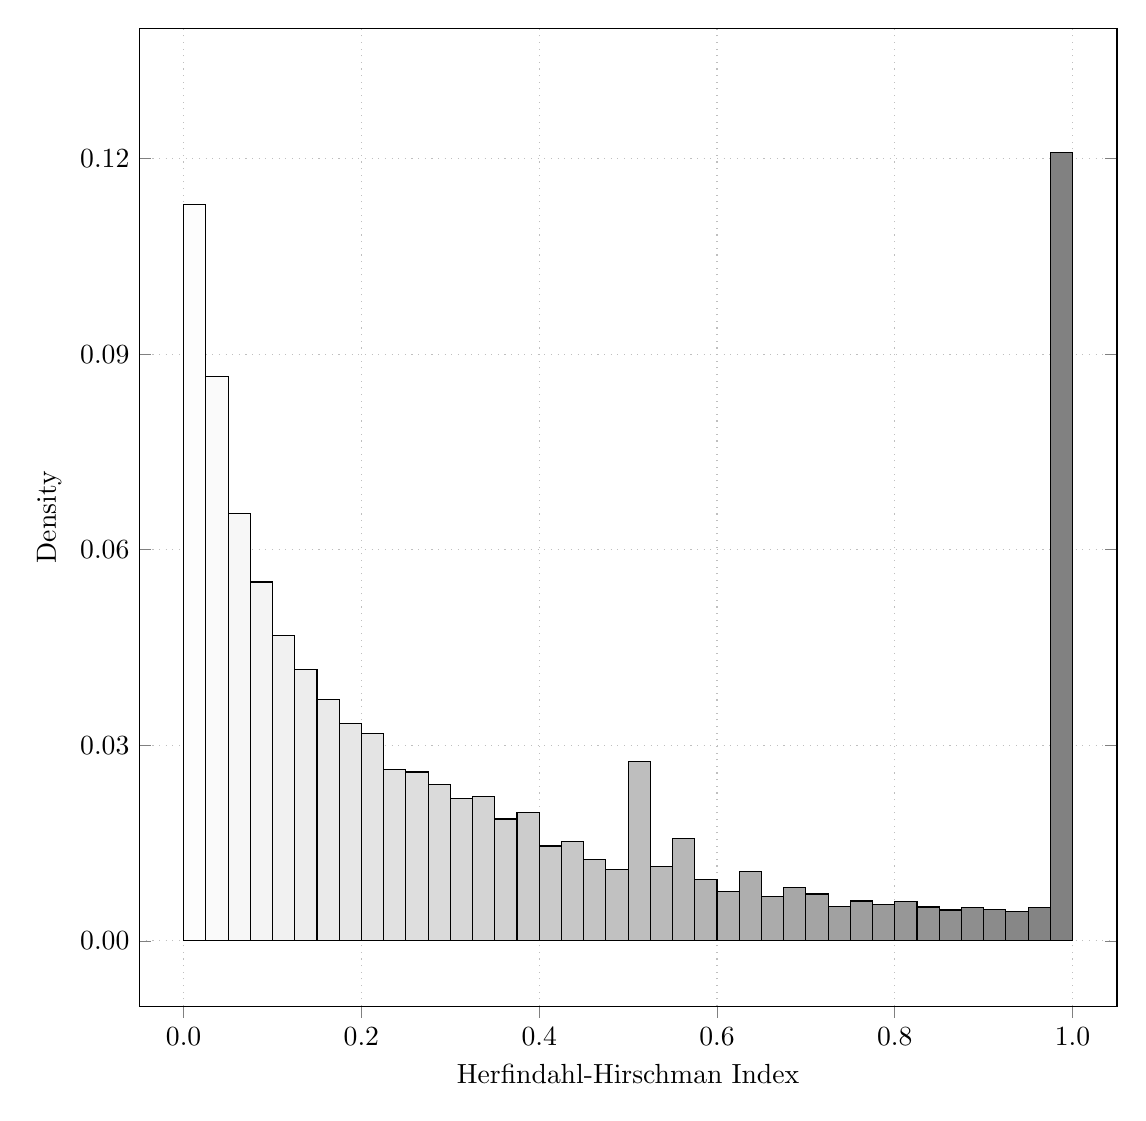
\begin{tikzpicture}
\pgfplotsset{set layers}
\begin{axis}[area style, xlabel=Herfindahl-Hirschman Index, ylabel=Density, xtick align=outside, xtick pos = left, height=14cm, width=14cm, xmin=-0.05, xmax=1.05, ymin = -0.01, ymax=0.14, ytick={0,0.03,0.06,0.09,0.12},xtick={0,0.2,0.4,0.6,0.8,1}, grid=major, set layers, major grid style = {dotted, /pgfplots/on layer=axis background}, legend pos = north east, y tick label style={/pgf/number format/.cd,fixed,fixed zerofill, precision=2,/tikz/.cd}, x tick label style={/pgf/number format/.cd,fixed,fixed zerofill, precision=1,/tikz/.cd}]
\addplot+[ybar interval, mark=no, color=black, fill=gray!1.25!white] plot coordinates { (0,.11292495) (.025,.08659977)};
\addplot+[ybar interval, mark=no, color=black, fill=gray!3.75!white] plot coordinates { (.025,.08659977) (.05,.06551824)};
\addplot+[ybar interval, mark=no, color=black, fill=gray!6.25!white] plot coordinates { (.05,.06551824) (.075,.05505403)};
\addplot+[ybar interval, mark=no, color=black, fill=gray!8.75!white] plot coordinates { (.075,.05505403) (.1,.04678795)};
\addplot+[ybar interval, mark=no, color=black, fill=gray!11.25!white] plot coordinates { (.1,.04678795) (.125,.04169323)};
\addplot+[ybar interval, mark=no, color=black, fill=gray!13.75!white] plot coordinates { (.125,.04169323) (.15000001,.03697815)};
\addplot+[ybar interval, mark=no, color=black, fill=gray!16.25!white] plot coordinates { (.15000001,.03697815) (.175,.0333139)};
\addplot+[ybar interval, mark=no, color=black, fill=gray!18.75!white] plot coordinates { (.175,.0333139) (.2,.03181631)};
\addplot+[ybar interval, mark=no, color=black, fill=gray!21.25!white] plot coordinates { (.2,.03181631) (.22499999,.02627903)};
\addplot+[ybar interval, mark=no, color=black, fill=gray!23.75!white] plot coordinates { (.22499999,.02627903) (.25,.02591197)};
\addplot+[ybar interval, mark=no, color=black, fill=gray!26.25!white] plot coordinates { (.25,.02591197) (.27500001,.02395714)};
\addplot+[ybar interval, mark=no, color=black, fill=gray!28.75!white] plot coordinates { (.27500001,.02395714) (.30000001,.02183662)};
\addplot+[ybar interval, mark=no, color=black, fill=gray!31.25!white] plot coordinates { (.30000001,.02183662) (.32499999,.02213445)};
\addplot+[ybar interval, mark=no, color=black, fill=gray!33.75!white] plot coordinates { (.32499999,.02213445) (.34999999,.01869043)};
\addplot+[ybar interval, mark=no, color=black, fill=gray!36.25!white] plot coordinates { (.34999999,.01869043) (.375,.01966575)};
\addplot+[ybar interval, mark=no, color=black, fill=gray!39.75!white] plot coordinates { (.375,.01966575) (.40000001,.01455425)};
\addplot+[ybar interval, mark=no, color=black, fill=gray!41.25!white] plot coordinates { (.40000001,.01455425) (.42500001,.01518349)};
\addplot+[ybar interval, mark=no, color=black, fill=gray!43.75!white] plot coordinates { (.42500001,.01518349) (.44999999,.01243162)};
\addplot+[ybar interval, mark=no, color=black, fill=gray!46.25!white] plot coordinates { (.44999999,.01243162) (.47499999,.01091936)};
\addplot+[ybar interval, mark=no, color=black, fill=gray!48.75!white] plot coordinates { (.47499999,.01091936) (.5,.02749765)};
\addplot+[ybar interval, mark=no, color=black, fill=gray!51.25!white] plot coordinates { (.5,.02749765) (.52499998,.01135773)};
\addplot+[ybar interval, mark=no, color=black, fill=gray!53.75!white] plot coordinates { (.52499998,.01135773) (.55000001,.01572253)};
\addplot+[ybar interval, mark=no, color=black, fill=gray!56.25!white] plot coordinates { (.55000001,.01572253) (.57499999,.00935046)};
\addplot+[ybar interval, mark=no, color=black, fill=gray!58.75!white] plot coordinates { (.57499999,.00935046) (.60000002,.00760538)};
\addplot+[ybar interval, mark=no, color=black, fill=gray!61.25!white] plot coordinates { (.60000002,.00760538) (.625,.01061313)};
\addplot+[ybar interval, mark=no, color=black, fill=gray!63.75!white] plot coordinates { (.625,.01061313) (.64999998,.00679576)};
\addplot+[ybar interval, mark=no, color=black, fill=gray!66.25!white] plot coordinates { (.64999998,.00679576) (.67500001,.00812974)};
\addplot+[ybar interval, mark=no, color=black, fill=gray!68.75!white] plot coordinates { (.67500001,.00812974) (.69999999,.00719008)};
\addplot+[ybar interval, mark=no, color=black, fill=gray!71.25!white] plot coordinates { (.69999999,.00719008) (.72500002,.00521008)};
\addplot+[ybar interval, mark=no, color=black, fill=gray!73.75!white] plot coordinates { (.72500002,.00521008) (.75,.00612038)};
\addplot+[ybar interval, mark=no, color=black, fill=gray!76.25!white] plot coordinates { (.75,.00612038) (.77499998,.00563796)};
\addplot+[ybar interval, mark=no, color=black, fill=gray!78.75!white] plot coordinates { (.77499998,.00563796) (.80000001,.00604277)};
\addplot+[ybar interval, mark=no, color=black, fill=gray!81.25!white] plot coordinates { (.80000001,.00604277) (.82499999,.00518701)};
\addplot+[ybar interval, mark=no, color=black, fill=gray!83.75!white] plot coordinates { (.82499999,.00518701) (.85000002,.00472976)};
\addplot+[ybar interval, mark=no, color=black, fill=gray!86.25!white] plot coordinates { (.85000002,.00472976) (.875,.00518072)};
\addplot+[ybar interval, mark=no, color=black, fill=gray!88.75!white] plot coordinates { (.875,.00518072) (.89999998,.004864)};
\addplot+[ybar interval, mark=no, color=black, fill=gray!91.25!white] plot coordinates { (.89999998,.004864) (.92500001,.00448856)};
\addplot+[ybar interval, mark=no, color=black, fill=gray!93.75!white] plot coordinates { (.92500001,.00448856) (.94999999,.00505697)};
\addplot+[ybar interval, mark=no, color=black, fill=gray!96.25!white] plot coordinates { (.94999999,.00505697) (.97500002,.12096869)};
\addplot+[ybar interval, mark=no, color=black, fill=gray!98.75!white] plot coordinates { (.97500002,.12096869) (1,.0001)};
\end{axis}
\end{tikzpicture}
}
\floatfoot{ \footnotesize \textsc{Note. ---} The figure displays a histogram to illustrate the distribution of labor market concentration in Germany. Labor market concentration refers to employment-based HHIs for combinations of NACE-4 industries and commuting zones and is tracked with annual frequency. HHI = Herfindahl-Hirschman Index. NACE-4 = 4-Digit Statistical Nomenclature of Economic Activities in the European Community. Source: IEB, 1999-2017.}
\end{figure}
}


\paragraph{Unit of Observation.} Unweighted HHI values obscure the share of workers and establishments that face labor markets with high concentration. When weighting the labor-market HHIs by employment, the mean HHI drops to 0.09, implying that the average employee works in a labor market with 11.1 equal employers. In contrast, the average establishment, with HHI equal to 0.03, encounters an equivalent of 30.3 competitors. Figure \ref{fig:C2} reports the cumulative distribution of HHIs for labor markets, workers and establishments. About 51.8 percent of all labor markets are highly concentrated as their HHI exceeds the threshold of 0.20 from E.U.\ antitrust policy. Overall, 12.8 percent of workers face high levels of labor market concentration, indicating that highly concentrated markets tend to be small labor markets. 3.5 percent of establishments operate in highly concentrated labor markets. But, by construction, this small share is a direct consequence of the HHI definition in which the existence of few firms implies high labor market concentration.

\paragraph{Alternative Labor Market Definitions.} In a next step, I examine the sensitivity of the baseline concentration measure to different labor market definitions, both in terms of the commercial and the geographical dimension. When adopting the broader 3-digit NACE classification, the average HHI drops to 0.26. Given this definition, 40.2 percent of all markets feature a high level of concentration. Conversely, the narrower 5-digit classification yields an increase in the mean HHI to 0.36. As expected, the fraction of highly concentrated markets becomes larger and equals 54.4 percent. I also construct HHIs for a spatial division into 401 administrative districts (3-digit NUTS regions), on which the delineation of commuting zones is based. District-level HHIs exhibit an average of 0.49 and a share of 70.6 percent in highly concentrated markets.



\paragraph{Alternative Objects and Subjects.} Parts of the literature rely on concentration of new hires or vacancies, arguing that flows more accurately capture the availability of jobs to workers than the stock of employment. Here, the difference between both concepts is small: along the entire distribution, new hires are slightly more concentrated than employment.\footnote{I define hires on the basis of the BHP concept of inflows, that is, the number of workers who work in an establishment on June 30 of the respective year but were not employed in the same establishment one year before. As marginal employment was not recorded in the IEB until 1998, the year 1999 does not allow for a differentiation between factual inflows and incumbent marginal workers appearing in the data for the first time. Measures of labor market concentration for hires therefore refer to the years 2000-2017.} Beyond, the existence of companies with more than one establishment leads to an underestimation of labor market concentration to the extent that establishments within the same company do not compete for workers \citep{MarinescuEtAl2021}. However, according to the IAB Establishment Panel, multi-establishment companies do not pose a major problem to the analysis as 72.7 percent of surveyed establishments constitute single-establishment companies.

\paragraph{Alternative Concentration Measures.} The HHI derives its popularity from the fact that, despite the simple calculation, it is able to reflect the two determinants of concentration: fewness of competitors and inequality of market shares. Specifically, the HHI is the arithmetic mean of market shares, with each of these shares being weighted by itself. The squaring of market shares assigns relatively high weights to large firms in the market (Curry/George, \citeyear{CurryGeorge1983}). To test its sensitivity, I calculate four alternative measures of absolute concentration that emphasize different aspects of the accumulation of workers on establishments: the Rosenbluth Index (RBI), the K-Subject Concentration Ratio (CRK), the Inverse Number of Subjects (INS) and the Exponential Index (EXP).\footnote{The formulas for the alternative concentration indices look as follows: \\[-0.6cm]
\begin{itemize}
\item Rosenbluth Index:\, $ RB\!I_{mt} =  1 \, / \, (  2\,\sum_{j=1}^{J} e_{jmt} \, j - 1 ) $
\item K-Subject Concentration Rate:\, $ C\!RK_{mt} =  \sum_{j=1}^{K} e_{jmt} $
\item Inverse Number of Subjects:\, $ I\!N\!S_{mt} =  1/J $
\item Exponential Index:\, $ E\!X\!P_{mt} = \prod_{j=1}^{J} e_{jmt}^{e_{jmt}} $
\end{itemize} \vspace*{-0.1cm}
where $j$ denotes the rank of firms in descending order of market shares.}

The Rosenbluth Index uses ranks of firms (in descending order of market shares) as weights, thus attributing less weight to larger firms (Rosenbluth, \citeyear{Rosenbluth1955}; Hall/Tideman, \citeyear{HallTideman1967}). On average, the Rosenbluth Index exhibits a value of 0.33 which falls slightly short of the corresponding HHI score. The K-Subject Concentration Ratio sums up the shares of the $K$ largest competitors in the market, thus applying weights of unity to a fixed set of market shares.\footnote{Due of their discrete nature, concentration ratios do not require information on the full population of firms.} On average, the largest establishment in the market holds an employment share of 43.7 percent. The median share accounts for 35.9 percent whereas the lower and upper quartile refer to shares of 16.4 and 66.7 percent in employment. The Inverse Number of Subjects contemplates measures concentration as the reciprocal of the number of competitors.\footnote{If competitors have equal size, the HHI collapses to $1/J$.} With a mean of 0.23, 4.4 establishments operate in an average labor market. But, the distribution is highly right-skewed with a median of only 0.08, equivalent to 13 establishments. Finally, the Exponential Index is the geometric mean of market shares weighted with themselves. Its average value amounts to 0.30 with an equivalent of 3.4 identical firms in the market.

\paragraph{Within- and Between-Variation.} In Figure \ref{fig:C3}, I investigate the development of labor market concentration in Germany over time. The average HHI remained relatively stable during the period of study. Between 1999 and 2017, there was a slight decrease in the average market-level HHI from 0.35 to 0.34. The four alternative concentration indices experience a similar trend. In contrast, concentration indices exhibit a markedly stronger variation between than within labor markets. To this end, Figure \ref{fig:C4} uses boxplots to visualize the distribution of labor market concentration by 4-digit NACE industries, pooled over commuting zones and years. Plausibly, widespread lines of business (such as restaurants, medical practices, retail trade or legal activities) constitute the least concentrated industries. Particularly low values of labor market concentration are also found for industries that relate to the following minimum wage sectors: hairdressing, roofing, painting and varnishing, and electrical trade. Conversely, highly specialized industries tend to show a greater degree of concentration, such as industries from the minimum wage sectors of waste removal, textile and clothing, and agriculture, forestry and gardening.

Figure \ref{fig:C5} illustrates that there is a strong heterogeneity across commuting zones. Moreover, the map in Figure \ref{fig:C6} visualizes average market-level HHIs for 3-digit NUTS regions. In addition, I enrich district-level HHIs with an urbanization indicator from the German Federal Office for Building and Regional Planning (BBSR). Average district-level HHIs indicate that labor markets in peripheral districts (0.51) are more concentrated than in metropolitan areas (0.47), providing an explanation for the urban wage premium.

%maybe add citation for city-wage premium

\paragraph{Comparison with Labor Supply Elasticities to the Firm.} In sum, the measures of labor market concentration point towards considerable monopsony power in German labor markets. Importantly, this result is consistent with studies that adopt a complementary approach and semi-structurally estimate wage elasticities of labor supply to the firm on related data from Germany. With values between 1.9 and 3.7, \citet{HirschEtAl2010} report elasticities that are far away from being perfectly elastic. Instead, the small magnitude mirrors an upward-sloping labor supply curve to the firm, implying that employers possess substantial monopsony power. In a similar fashion, \citet{BachmannFrings2017} study heterogeneity in monopsony power across German industries and document that the majority of elasticities falls in the range between 0.5 and 3. Finally, the finding that labor market concentration is lower in urban than in rural areas augments evidence on Germany from \citet{HirschEtAl2020} who show that the wage elasticity of labor supply to the firm increases in population density.







\section{Effects of Labor Market Concentration}
\label{sec:6}

In a next step, I explore whether firms - prior to minimum wage regulations - reduce earnings and employment in more concentrated labor markets, as postulated by monopsony theory. Such a negative interrelation is an important piece of evidence for the monopsony argument because, in the absence of monopsonistic exploitation, there is no reason why minimum wage effects should vary between slightly and highly concentrated labor markets.

\paragraph{Empirical Model.}

To study the effect of labor market concentration on the outcome variables of interest, I estimate the following econometric model
\begin{equation}
\label{eq:2}
ln\,Y_{jizt} \,=\,  \theta \cdot ln\,H\!H\!I_{izt}  \,+\, \delta_{j}  \,+\, \zeta_{zt}  \,+\, \varepsilon_{jizt}
\end{equation}
where $Y$ refers either to average earnings or employment per firm $j$ in year $t$, $H\!H\!I$ is the corresponding Herfindahl-Hirschman Index, $\delta_{j}$ and $\zeta_{zt}$ are  establishment and commuting-zone-by-year fixed effects, and $\varepsilon$ is an error term. Depending on the sector, I keep only those establishment-year observations before minimum wage regulations came into effect (see Table \ref{tab:B2} for the sector-specific timing of minimum wage implementations).\footnote{As a consequence, the sectors of main construction, electrical trade and roofing do not enter the specification as sectoral minimum wages were implemented ahead of 1999.} Thus, the period of analysis refers to the years 1999-2014. In a first specification, I condition on establishment fixed effects to capture unobserved time-invariant heterogeneity across employers. Thus, the identification of elasticity estimates $\hat{\theta}$ stems from variation within establishments over time. In a second regression, I add year fixed effects to account for time-specific events common to all establishments, e.g., the business cycle. I cluster standard errors at the labor-market level.

The main threat of identification are time-varying variables that correlate with HHI and have an impact on establishment-level earnings and/or employment. Specifically, labor demand or labor supply shocks may bias the estimation. For instance, a positive productivity shock will make incumbent firms increase earnings and employment along the labor supply curve while new entrants simultaneously lower the HHI, creating a downward bias. Therefore, in a third specification, I condition on year-by-commuting-zone fixed effects to absorb the local dimension of these threats.

Nevertheless, the question remains whether demand or supply shocks specific to a certain labor market within a commuting zone may skew the results. Moreover, when estimating employment effects, simultaneity bias might arise from the mechanical effect of employment on the employment-based HHI \citep{MarinescuEtAl2021}. To rule out these issues of endogeneity, I follow the instrumental variable strategy from \citet{AzarEtAl2017} in a fourth and baseline specification. Specifically, I instrument any HHI value in a certain commuting zone $c$ by the average of the log inverse number of firms in all other commuting zones for the same industry and time period:
\begin{equation}
\label{eq:3}
\overline{ln\,I\!N\!S}^{\,-c}_{it} \,=\,  \frac{\sum_{z \neq c\vphantom{/}} \, ln\,I\!N\!S_{izt}}{Z-1} \,=\, \frac{\sum_{z \neq c\vphantom{/}} \, ln\,J^{-1}_{izt}}{50}
\end{equation}
Favorably, the ``leave-one-out'' property of this instrument delivers variation in local labor market concentration that is driven by national, non-local forces in the respective industry and, thus, not by shifts in the industry in that certain commuting zone. As such, the instrument rules out omitted variable bias from local shocks that both affect labor market concentration and the outcome variable. Nevertheless, the instrument is not fully exogenous when shocks are correlated across regions (e.g., from national shocks). The exogeneity assumption is violated when the instrument exerts an additional direct effect, $\Phi\neq0$, on the outcome variable in the second-stage regression (i.e., other than through labor market concentration).\footnote{When allowing for instrument endogeneity, the second-stage regression takes the following form: \begin{equation*} ln\,Y_{jizt} \,=\,  \theta \cdot \widehat{ln\,H\!H\!I}_{izt} \,+\, \Phi \cdot \overline{ln\,I\!N\!S}^{\,-c}_{it}  \,+\, \delta_{j}  \,+\, \zeta_{zt}  \,+\, \varepsilon_{jizt} \end{equation*}.} To assess the magnitude of the potential bias, I formulate a range of values for this direct effect between zero (exogeneity) and the estimated reduced-form coefficient. Given this range, I apply the plausibly exogenous regression method \citep{ConleyEtAl2012} to derive bounds for the causal effect of labor market concentration on the outcomes of interest.








\paragraph{Effects of Labor Market Concentration on Earnings.} In line with monopsony theory, the results indicate that, prior to minimum wage regulations, higher labor market concentration is associated with significantly lower earnings. Table \ref{tab:2} displays the estimated effects of labor market concentration on log average daily wages of regular full-time workers per firm. In the first regression, with mere establishment fixed effects, I find that an increase in HHI by 10 percent is ceteris paribus associated with a reduction in mean earnings by 0.3 percent. In Columns (2) and (3), this effect weakens to 0.1 percent when adding year or year-by-commuting-zone fixed effects. The similarity of the estimates in the second and third specification indicate that local shocks do not pose a problem to the identification. To allow for a causal interpretation, the baseline specification in Column (4) carries out the IV estimation with (\ref{eq:3}) as instrumental variable. The respective F statistic is 430.8 which validates the relevance of the instrument.\footnote{Favorably, the first-stage regression of HHI on the instrument shows the expected positive sign ($\plus$0.8).} The IV estimate is still negative but larger in absolute terms: an increase in HHI by 10 percent reduces average earnings in the firm by 0.5 percent. Put differently, a decrease in the equivalent number of employers from 10 (HHI=0.1) to 5 (HHI=0.2) firms in the labor market is associated with a decline in earnings by 5 percent. Across specifications, all elasticities are significantly different from zero at 1 percent levels.



%\afterpage{
\begin{table}[!ht]
\centering
%\resizebox{\textwidth}{!}{
\scalebox{0.90}{
\begin{threeparttable}
\caption{Effects of LM Concentration on Earnings}
\label{tab:2}
\begin{tabular}{|C{4cm}|C{2.7cm}C{2.7cm}C{2.7cm}C{2.7cm}|} \hline \hline
\multirow{4}{*}{\diagbox[height=4.4175\line, innerwidth=4cm]{Regressor}{\shortstack{ \\ \hspace{0.1cm}Dependent \\ \hspace{0.1cm}Variable }}} & \multirow{4.4}{*}{\shortstack{(1) \\ Log \\ Mean Daily\vphantom{/} \\ Wages }} & \multirow{4.4}{*}{\shortstack{(2) \\ Log \\ Mean Daily\vphantom{/} \\ Wages }} & \multirow{4.4}{*}{\shortstack{(3) \\ Log \\ Mean Daily\vphantom{/} \\ Wages }} & \multirow{4.4}{*}{\shortstack{(4) \\ Log \\ Mean Daily\vphantom{/} \\ Wages }} \\
&&&& \\
&&&& \\
&&&& \\[0.2cm] \hline
\multirow{2.4}{*}{Log HHI} &  \multirow{2.4}{*}{\shortstack{\hphantom{***}-0.025***\hphantom{-}  \\ (0.007)}}  & \multirow{2.4}{*}{\shortstack{\hphantom{***}-0.014***\hphantom{-}  \\ (0.004)}} & \multirow{2.4}{*}{\shortstack{\hphantom{***}-0.014***\hphantom{-}  \\ (0.004)}} & \multirow{2.4}{*}{\shortstack{\hphantom{***}-0.046***\hphantom{-}  \\ (0.006)}}   \\
&&&& \\[0.2cm] \hdashline
&&&& \\[-0.2cm]
Instrument  & None & None & None & $ \overline{\text{Log}\,\,\text{INS}} \,\,\backslash\, \{c\} $  \\
\multirow{2.4}{*}{\shortstack{Fixed \\ Effects}}  & \multirow{2.4}{*}{Establishment} &  \multirow{2.4}{*}{\shortstack{Establishment \\ Year}} & \multirow{2.4}{*}{\shortstack{Establishment \\ Year $\times$ CZ}} &  \multirow{2.4}{*}{\shortstack{Establishment \\ Year $\times$ CZ}} \\
&&&& \\
\multirow{3.4}{*}{\shortstack{Labor Market \\ Definition \\ (Object)}}  & \multirow{3.4}{*}{\shortstack{NACE-4 \\ $\times$ CZ \\ (Employment)}} & \multirow{3.4}{*}{\shortstack{NACE-4 \\ $\times$ CZ \\ (Employment)}} & \multirow{3.4}{*}{\shortstack{NACE-4 \\ $\times$ CZ \\ (Employment)}} & \multirow{3.4}{*}{\shortstack{NACE-4 \\ $\times$ CZ \\ (Employment)}} \\
&&&& \\
&&&& \\[0.2cm] \hdashline
&&&& \\[-0.2cm]
Observations &  2,139,426       & 2,139,426       & 2,139,426       & 2,139,426         \\[0.2cm]
Adjusted R$^2$ &  0.836    & 0.845    &   0.845    &      \\[0.2cm]
F Statistic &  &  &  & 430.8 \\[0.2cm]  \hline \hline
\end{tabular}
\begin{tablenotes}
\item \footnotesize \textsc{Note. ---} The table displays fixed effects regressions of log establishment-level means of daily wages (of regular full-time workers) on the log of HHI. The instrumental variable refers to the leave-one-out industry average of the log inverse number of firms across commuting zones. Standard errors (in parentheses) are clustered at the labor-market level. CZ = Commuting Zone. HHI = Herfindahl-Hirschman Index. INS = Inverse Number of Subjects. LM = Labor Market. NACE-4 = 4-Digit Statistical Nomenclature of Economic Activities in the European Community. * = p$<$0.10. ** = p$<$0.05. *** = p$<$0.01. Sources: IEB $\plus$ BHP, 1999-2014.
\end{tablenotes}
\end{threeparttable}
}
\end{table}
%}



To test the sensitivity of the earnings effect, I carry out the IV specification with alternative labor market definitions (Table \ref{tab:D1}) and concentration indices (Table \ref{tab:D2}). The use of 3- and 5-digit NACE industries or 3-digit NUTS regions results in slightly more negative coefficients. In contrast, the configuration with a HHI based on hires instead of employment leaves the estimate unaltered. The same holds true for specifications that replace the HHI by the Rosenbluth Index, the Inverse Number of Subjects or the Exponential Index. The 1-Subject Concentration Ratio also delivers a negative but more pronounced effect on earnings.

Table \ref{tab:D3} shows separate regressions by West Germany and East Germany (including the City of Berlin). Importantly, the negative effect of labor market on earnings manifests in both parts of the country. In Table \ref{tab:D4}, I explore whether the effect of labor market concentration varies at different percentiles of the earnings distribution in a firm. The results indicate that a 10 percent increase in HHI reduces the 25th percentile by 0.2 percent, the median by 0.4 percent and the 75th percentile by 0.6 percent. Hence, labor market concentration enables firms to push down large portions of the wage distribution, with greater monopsonistic exploitation at the top than at the bottom end of the distribution. This heterogeneity mirrors related evidence that non-routine cognitive workers in Germany are subject to a higher degree of monopsony power than routine or non-routine manual workers \citep{BachmannEtAl2021}.

In a further robustness check, I explore whether the relationship between labor market concentration and earnings depends on the degree of outward mobility in a labor market. For each labor market, I define outward mobility as the share of workers who take up a new job in another labor market when leaving the job at their previous establishment.\footnote{More formally, the share is computed as follows: $\text{outward mobility}_{izt} = \text{movers}_{izt} \,/\, (\text{stayers}_{izt} + \text{movers}_{izt})$ where ``stayers'' (``movers'') are workers who leave their previous establishment in $t$ and take up a new job in $t+1$ at another establishment in the same (another) labor market. To construct this measure, I use information on only the main job per worker and year.} With a value of 64.9 percent, the average degree of outward mobility is relatively high. In a next step, I segment the regression sample into three groups based on the intensity of outward mobility within a labor market.\footnote{Within each minimum wage sector, I separate firms into three tercile groups based on the average outward mobility within their labor market. The average intensity of outward mobility by group is: 61.0 percent (low mobility), 66.1 percent (medium mobility), and 73.4 percent (high mobility).} Table \ref{tab:D5} shows the regression results by degree of outward mobility. As expected, the negative impact of higher labor market concentration on earnings becomes weaker when outward mobility increases. Hence, firms in highly concentrated labor markets can lowers earnings more strongly when workers find it more difficult to get a job in another labor market. The elasticity for the low mobility group turns out to be almost twice as high as in the high mobility group. Importantly, however, the negative impact on earnings features a substantial order of magnitude even when outward mobility is high. The documented impact of outward mobility on the HHI-earnings relationship is similar to that found for U.S.\ occupational labor markets by \citet{SchubertEtAl2020}.


\paragraph{Effects of Labor Market Concentration on Employment.} Theory of imperfect competition suggests that, absent any regulation, employers with labor market power reduce earnings by shortening employment along the labor supply curve to the firm. To see whether the negative effect on earnings in highly concentrated labor markets also goes along with lower employment, I re-run the four specifications of Equation (\ref{eq:2}) with log employment of regular full-time workers as the outcome variable. Table \ref{tab:3} displays the results. Indeed, all three OLS specifications arrive at a negative HHI coefficient around -0.05, indicating that firms employ significantly less workers in concentrated vis-\`{a}-vis unconcentrated labor markets. Once again, the baseline IV estimation in Column (4) shows a larger effect size: an increase in HHI by 10 percent makes firms reduce their employment of regular full-time workers by 1.6 percent. All reported effects are significantly different from zero.

\afterpage{
\begin{table}[!ht]
\centering
%\resizebox{\textwidth}{!}{
\scalebox{0.90}{
\begin{threeparttable}
\caption{Effects of LM Concentration on Employment}
\label{tab:3}
\begin{tabular}{|C{4cm}|C{2.7cm}C{2.7cm}C{2.7cm}C{2.7cm}|} \hline \hline
\multirow{4}{*}{\diagbox[height=4.4175\line, innerwidth=4cm]{Regressor}{\shortstack{ \\ \hspace{0.1cm}Dependent \\ \hspace{0.1cm}Variable }}} & \multirow{4.4}{*}{\shortstack{(1) \\ Log \\ Regular FT\vphantom{/} \\ Employment }} & \multirow{4.4}{*}{\shortstack{(2) \\ Log \\ Regular FT\vphantom{/} \\ Employment }} & \multirow{4.4}{*}{\shortstack{(3) \\ Log \\ Regular FT\vphantom{/} \\ Employment }} & \multirow{4.4}{*}{\shortstack{(4) \\ Log \\ Regular FT\vphantom{/} \\ Employment }} \\
&&&& \\
&&&& \\
&&&& \\[0.2cm] \hline
\multirow{2.4}{*}{Log HHI} &  \multirow{2.4}{*}{\shortstack{\hphantom{***}-0.050***\hphantom{-}  \\ (0.012)}}  & \multirow{2.4}{*}{\shortstack{\hphantom{***}-0.055***\hphantom{-}  \\ (0.011)}} & \multirow{2.4}{*}{\shortstack{\hphantom{***}-0.058***\hphantom{-}  \\ (0.011)}} & \multirow{2.4}{*}{\shortstack{\hphantom{***}-0.156***\hphantom{-}  \\ (0.018)}}   \\
&&&& \\[0.2cm] \hdashline
&&&& \\[-0.2cm]
Instrument  & None & None & None & $ \overline{\text{Log}\,\,\text{INS}} \,\,\backslash\, \{c\} $  \\
\multirow{2.4}{*}{\shortstack{Fixed \\ Effects}}  & \multirow{2.4}{*}{Establishment} &  \multirow{2.4}{*}{\shortstack{Establishment \\ Year}} & \multirow{2.4}{*}{\shortstack{Establishment \\ Year $\times$ CZ}} &  \multirow{2.4}{*}{\shortstack{Establishment \\ Year $\times$ CZ}} \\
&&&& \\
\multirow{3.4}{*}{\shortstack{Labor Market \\ Definition \\ (Object)}}  & \multirow{3.4}{*}{\shortstack{NACE-4 \\ $\times$ CZ \\ (Employment)}} & \multirow{3.4}{*}{\shortstack{NACE-4 \\ $\times$ CZ \\ (Employment)}} & \multirow{3.4}{*}{\shortstack{NACE-4 \\ $\times$ CZ \\ (Employment)}} & \multirow{3.4}{*}{\shortstack{NACE-4 \\ $\times$ CZ \\ (Employment)}} \\
&&&& \\
&&&& \\[0.2cm] \hdashline
&&&& \\[-0.2cm]
Observations &  2,139,426       & 2,139,426       & 2,139,426       & 2,139,426         \\[0.2cm]
Adjusted R$^2$ &  0.898    & 0.898    &   0.898    &      \\[0.2cm]
F Statistic &  &  &  & 430.8 \\[0.2cm]  \hline \hline
\end{tabular}
\begin{tablenotes}
\item \footnotesize \textsc{Note. ---} The table displays fixed effects regressions of log establishment-level employment (of regular full-time workers) on the log of HHI. The instrumental variable refers to the leave-one-out industry average of the log inverse number of firms across commuting zones. Standard errors (in parentheses) are clustered at the labor-market level. CZ = Commuting Zone. FT = Full-Time. HHI = Herfindahl-Hirschman Index. INS = Inverse Number of Subjects. LM = Labor Market. NACE-4 = 4-Digit Statistical Nomenclature of Economic Activities in the European Community. * = p$<$0.10. ** = p$<$0.05. *** = p$<$0.01. Sources: IEB $\plus$ BHP, 1999-2014.
\end{tablenotes}
\end{threeparttable}
}
\end{table}
}



Again, I examine the robustness of the baseline employment effects with respect to different labor market definitions (Table \ref{tab:D6}) and concentration measures (Table \ref{tab:D7}). The effect of labor market concentration on employment remains unchanged for 5-digit NACE industries or hires-based HHIs but becomes even larger when adopting 3-digit NACE industries or 3-digit NUTS regions. The latter also applies for the 1-Subject Concentration Ratio whereas the Rosenbluth Index, the Inverse Number of Subjects and the Exponential Index exhibit a similar reduction in employment.

Table \ref{tab:D8} displays that the negative impact of HHI on employment holds both for West and East German firms. Until now, the analysis has focused on the employment of regular full-time workers. In Table \ref{tab:D9}, I provide employment effects for groups of workers for which no wage measure is available in the data. Importantly, I also arrive at a similarly negative effect of labor market concentration on overall employment, which is the sum of regular full-time, regular part-time, and marginal part-time workers. Moreover, the regressions point out that firms also reduce employment of regular part-time and marginal part-time workers in highly concentrated labor markets. Table \ref{tab:D10} presents elasticities by different intensities of outward mobility. The negative impact of labor market concentration on employment becomes less pronounced when outward mobility is high. As with earnings, the elasticity for the low mobility group is about twice as negative as for the high mobility group.



\paragraph{Causal Interpretation.} Acknowledging that the instrument might not be fully exogenous, I follow Conley et al.'s \citeyearpar{ConleyEtAl2012} plausibly exogenous regression technique to derive upper and lower bounds for the causal effect of higher labor market concentration on earnings and employment in Table \ref{tab:D11}. The reduced-form regression (i.e., the regression of the earnings variable on the instrument) yields a coefficient of -0.038.\footnote{The reduced-form regression is as follows: $ln\,Y_{jizt} \,=\,  \Phi^{\text{min}} \cdot \overline{ln\,I\!N\!S}^{\,-c}_{it}  \,+\, \delta_{j}  \,+\, \zeta_{zt}  \,+\, \varepsilon_{jizt}$.} This coefficient reflects the maximum of instrument endogeneity that can enter the second-stage regression of the earnings variable on the first-stage variation in labor market concentration. Under the assumption that the instrument's direct effect on earnings in the second stage ranges between zero (full exogeneity) and -0.038 (reduced-form effect), the bounds for the second-stage effect of labor market concentration on earnings range between -0.051 and 0.010. The causal effect of labor market concentration on earnings is negative provided that the direct effect of the instrument on earnings in the second stage is greater than -0.029, or smaller than 77.3 (=0.029/0.038) percent of the reduced-form effect. Hence, the negative effect of labor market concentration on earnings holds even for a large degree of instrument endogeneity. The plausible interval for the second-stage effect of HHI on employment ranges between -0.173 and 0.032. Accordingly, the true effect of labor market concentration on employment is less than zero provided that the size of the instrument's direct effect on employment in the second stage is smaller than 79.0 (=0.101/0.128) percent of the reduced-form effect. Again, the negative effect of labor market concentration on employment is robust to substantial endogeneity of the instrument.

Industry-based measures of local labor market concentration might pick up product market concentration unless the latter has a national rather than a local dimension \citep{Manning2021}. Under imperfect competition in product markets, firms with monopoly power will lower output and employment \citep{MarinescuEtAl2021} but, absent any monopsony power, wages remain tied to marginal productivity along an infinitely elastic labor supply curve to the firm. In the presence of rent sharing, however, monopolists will pass on parts of their profits to their employees, thus paying higher wages (Qiu/Sojourner, \citeyear{QiuSojourner2019}). Hence, if product market concentration was the causal driver of the negative HHI effects on employment, the wage regressions would display zero or positive effects of higher labor market concentration. Yet, the fact that not only the employment but also the wage regressions feature negative coefficients endorses the conjecture that it is not product but labor market power that enables firms to reduce their employment. As an additional check, Table \ref{tab:D12} shows that the results are not sensitive to excluding the service sectors where product markets tend to have more of a local nature.\footnote{To be precise, I discard the sectors of commercial cleaning, waste removal, nursing care, security, temporary work, hairdressing, and chimney sweeping.}

By and large, I document robust evidence that firms employ less workers at lower wage levels when operating in more concentrated labor markets. The finding that higher labor market concentration reduces both earnings and employment in a firm corroborates the predictions of monopsony theory in a sense that employers with labor market power suppress wages along a positive sloped labor supply curve to the firm. Division of the baseline employment elasticity by the respective earnings elasticity yields a wage elasticity of labor supply of 3.4 (=0.156/0.046). Albeit conceptually different, the coefficient has a magnitude similar to estimated wage elasticities of labor supply to the single firm from dynamic monopsony models on Germany (see Section \ref{sec:5}).



\section{Minimum Wage Effects}
\label{sec:7}

The previous analysis indicates that, absent minimum wage regulations, firms in concentrated labor markets suppress workers' wages by constraining their employment. Importantly, monopsony theory expects reasonably-set minimum wages to counteract such monopsonistic exploitation without having negative effects on employment. Although this line of reasoning is frequently brought up to rationalize close-to-zero minimum wage effects on employment, direct evidence for the monopsony argument is rare. In the following, I perform empirical tests regarding the role of monopsony power on minimum wage effects. Given the concentration indices, I examine whether sectoral minimum wages exhibit less adverse employment effects in imperfectly competitive labor markets where concentration tends to be higher.


\paragraph{Empirical Model.} The empirical analysis of minimum wage effects proceeds in two steps. In a first step, I test whether sectoral minimum wages effectively raise earnings. An empirical bite confirmation is an essential prerequisite because causal effects will not manifest unless minimum wages are binding.\footnote{In default of a bite, near-zero minimum wage effects on employment would have a fundamentally different implication relative to a setting with binding minimum wages.} Provided that there is a significant bite, I examine the minimum wage effects on employment in a second step. In both cases, the baseline version of the regression model takes the following log-linear form
\begin{equation}
\label{eq:4}
ln\,Y_{jsizt} \,=\,  \alpha \cdot ln\,w^{min}_{st}\, + \, \beta \cdot ln\,w^{min}_{st} \cdot \overline{H\!H\!I}_{iz}  \, + \,  X^{T}_{st} \,  \gamma \,+\, \delta_{j}  \,+\, \zeta_{zt}  \,+\, \varepsilon_{jsizt}
\end{equation}
where the outcome variable $Y$ refers to either average daily earnings or employment in establishment $j$ for year $t$, $w^{min}$ is the prevailing minimum wage in sector $s$, $H\!H\!I$ is the respective Herfindahl-Hirschman Index, $X$ is the set of control variables, $\delta_{j}$ and $\zeta_{zt}$ are fixed effects, and $\epsilon$ is the error term.\footnote{For the sake of simplicity, the notation in (\ref{eq:4}) disregards that minimum wages differ regionally in some sectors. If so, minimum wages are usually set differently for West Germany, East Germany, and the City of Berlin. In the security sector for 2011-2013, minimum wages vary by federal state.} Specifically, I infer establishment responses to minimum wages from regressing the logarithm of the outcome variable on the logarithm of the current minimum wage in the sector. To test the moderating role of labor market concentration, I add an interaction effect with HHI for the labor market in which the establishment is operating. Thus, the estimate for the minimum wage elasticity on earnings or employment, as a function of HHI, reads: $\hat{\eta}^{\,Y}_{w^{min}} \,=\, \hat{\alpha} + \hat{\beta} \cdot H\!H\!I $. Standard errors are clustered at the labor-market level.

As in Section \ref{sec:6}, I successively include establishment fixed effects, year fixed effects, and year-by-commuting-zone fixed effects in a first, second, and third specification of (\ref{eq:4}) to absorb unobserved time-invariant heterogeneity and local shocks. \citet{HaucapEtAl2011} and \citet{BachmannEtAl2014} discuss strategic behavior of unions and employer associations under the possibility of coverage extension for CBAs in Germany. Hence, in a fourth and baseline specification, I address potential endogeneity in minimum wage legislation using a set of sectoral control variables: the sectoral share of establishments subject to CBAs and the logarithm of employment by sector and territory (i.e., by West Germany, East Germany, and the City of Berlin). In the spirit of \citet{AllegrettoEtAl2011}, I further control for sector-specific linear time trends to grasp heterogeneous paths of growth in the outcome variable.




%The main variable of interest is the interaction term. Specifically, ...
Across all four specifications, I construct the interaction term as a product of the sectoral minimum wage level and an establishment-specific average of HHI across available years. The use of averaged HHIs is useful for two reasons: First, my paramount objective is to examine minimum wage effects within establishments at given values of labor market concentration. However, in a panel context, demeaning an interaction effect of two time-varying regressors yields a combination of mutual between- and within-unit interdependencies of both variables (Giesselmann/Schmidt-Catran, \citeyear{GiesselmannSchmidtCatran2020}). Yet, averaging over HHI will ensure that the interaction effect captures solely the moderating effect of level differences in HHI on within-unit variation in minimum wages. Second, the use of mean HHIs alleviates two threats of identification: reverse causality between employment and HHI as well as the confounding impact of non-local labor market shocks on HHI. On the downside, however, averaging over HHI will give rise to endogeneity in case minimum wage changes correlate with HHI levels. To this end, I regress HHI values on sectoral minimum wages to inspect the correlation between both variables conditional on the covariates from the baseline specification. Reassuringly, the variables do not exhibit any correlation at all (p=0.90), thus alleviating the concern that using HHI averages might induce endogeneity (see Table \ref{tab:E1}).





\paragraph{Minimum Wage Effects on Earnings.} Before turning to employment effects, it is necessary to verify whether the minimum wages actually heightened wages. To this end, I run Equation (\ref{eq:4}) on the data, with the logarithm of mean daily wages of regular full-time workers per firm as the outcome variable. Table \ref{tab:4} displays the estimated minimum wage effects on earnings by market form. Across all four specifications, the regressions demonstrate that increases in sectoral minimum wages were binding, regardless of the underlying market form. Column (4) relates to the baseline specification that includes establishment and year-by-commuting-zone fixed effects as well as control variables. In competitive labor markets with zero HHI, a 10 percent rise in minimum wages leads ceteris paribus to an average increase in mean daily earnings by 0.7 percent. In line with the evidence on monopsonistic exploitation, the earnings effect becomes more positive in more concentrated labor markets where wages are increasingly set below marginal productivity.\footnote{In a similar fashion, \citet{FuestEtAl2018} find that monopsony power moderates the impact of local business tax rates on wages.} Specifically, in the polar case of a monopsonistic labor market with HHI equal to one, a rise in minimum wages by 10 percent results in an increase in earnings by 3.3 percent. Both the main effect, the interaction effect and the resulting minimum wage elasticities on earnings are significantly different from zero.

\afterpage{
\begin{table}[!ht]
\centering
%\resizebox{\textwidth}{!}{
\scalebox{0.90}{
\begin{threeparttable}
\caption{Minimum Wage Effects on Earnings}
\label{tab:4}
\begin{tabular}{|C{4cm}|C{2.7cm}C{2.7cm}C{2.7cm}C{2.7cm}|} \hline \hline
\multirow{4}{*}{\diagbox[height=4.4175\line, innerwidth=4cm]{Regressor}{\shortstack{ \\ \hspace{0.1cm}Dependent \\ \hspace{0.1cm}Variable }}} & \multirow{4.4}{*}{\shortstack{(1) \\ Log \\ Mean Daily\vphantom{/} \\ Wages }} & \multirow{4.4}{*}{\shortstack{(2) \\ Log \\ Mean Daily\vphantom{/} \\ Wages }} & \multirow{4.4}{*}{\shortstack{(3) \\ Log \\ Mean Daily\vphantom{/} \\ Wages }} & \multirow{4.4}{*}{\shortstack{(4) \\ Log \\ Mean Daily\vphantom{/} \\ Wages }} \\
&&&& \\
&&&& \\
&&&& \\[0.2cm] \hline
\multirow{2.4}{*}{Log Minimum Wage} &  \multirow{2.4}{*}{\shortstack{\hphantom{***}0.689***  \\ (0.016)}}  & \multirow{2.4}{*}{\shortstack{\hphantom{***}0.077***  \\ (0.018)}} & \multirow{2.4}{*}{\shortstack{\hphantom{**}0.045**  \\ (0.018)}} & \multirow{2.4}{*}{\shortstack{\hphantom{***}0.074***  \\ (0.014)}}   \\
                                                                                                                                                                                                                    &&&&  \\
\multirow{2.4}{*}{\shortstack{Log Minimum Wage \\ $\times$ $\overline{\text{HHI}}$}} &  \multirow{2.4}{*}{\shortstack{\hphantom{***}0.733*** \\ (0.109)}}  & \multirow{2.4}{*}{\shortstack{\hphantom{***}0.382*** \\ (0.090)}} & \multirow{2.4}{*}{\shortstack{\hphantom{***}0.263*** \\ (0.071)}} & \multirow{2.4}{*}{\shortstack{\hphantom{***}0.260*** \\ (0.063)}}    \\
&&&& \\[0.2cm] \hdashline
&&&& \\[-0.2cm]
Control Variables  & No & No  & No & Yes \\
\multirow{2.4}{*}{\shortstack{Fixed \\ Effects}}  & \multirow{2.4}{*}{Establishment} &  \multirow{2.4}{*}{\shortstack{Establishment \\ Year}} & \multirow{2.4}{*}{\shortstack{Establishment \\ Year $\times$ CZ}} &  \multirow{2.4}{*}{\shortstack{Establishment \\ Year $\times$ CZ}} \\
&&&& \\
\multirow{3.4}{*}{\shortstack{Labor Market \\ Definition \\ (Object)}}  & \multirow{3.4}{*}{\shortstack{NACE-4 \\ $\times$ CZ \\ (Employment)}} & \multirow{3.4}{*}{\shortstack{NACE-4 \\ $\times$ CZ \\ (Employment)}} & \multirow{3.4}{*}{\shortstack{NACE-4 \\ $\times$ CZ \\ (Employment)}} & \multirow{3.4}{*}{\shortstack{NACE-4 \\ $\times$ CZ \\ (Employment)}} \\
&&&& \\
&&&& \\[0.2cm] \hdashline
&&&& \\[-0.2cm]
Observations &  2,700,155    & 2,700,155    & 2,700,155    & 2,700,155      \\[0.2cm]
Adjusted R$^2$ &  0.799    & 0.810    &   0.811    & 0.811      \\[0.2cm] \hline \hline
\end{tabular}
\begin{tablenotes}
\item \footnotesize \textsc{Note. ---} The table displays fixed effects regressions of log establishment-level means of daily wages (of regular full-time workers) on log sectoral minimum wages as well as their interaction effect with labor market concentration (measured as average HHI). The set of control variables includes log overall employment per sector-by-territory combination, the sectoral share of establishments subject to a collective bargaining agreement, and sector-specific linear time trends. Standard errors (in parentheses) are clustered at the labor-market level. CZ = Commuting Zone. HHI = Herfindahl-Hirschman Index. NACE-4 = 4-Digit Statistical Nomenclature of Economic Activities in the European Community. * = p$<$0.10. ** = p$<$0.05. *** = p$<$0.01. Sources: IEB $\plus$ BHP $\plus$ IAB Establishment Panel, 1999-2017.
\end{tablenotes}
\end{threeparttable}
}
\end{table}
}


Table \ref{tab:E2} illustrates minimum wage elasticities of earnings separately for West Germany and East Germany. Sectoral minimum wage increases result in significant wage growth in both parts of the country. West Germany exhibits less pronounced main effects than East Germany where both earnings and wage floors tend to be lower. Both interactions effect turn out to be positive but only the coefficient for West Germany remains significant.

First and foremost, minimum wages push up earnings at the bottom of the wage distribution. Hence, lower percentiles of the wage distribution are supposed to show accordingly larger effects on earnings. Table \ref{tab:E3} displays minimum wage effects on the 25th percentile, the median, and the 75th percentile of the wage distribution of regular full-time workers within establishments. In unconcentrated labor markets, a minimum wage increase by 10 percent significantly raises the 25th percentile of the wage distribution by 1.3 percent. As expected, this effect weakens for higher percentiles of the distribution where earnings increasingly exceed wage floors: an analogous minimum wage increase moves the median wage by 0.8 percent and the 75th percentile of the wage distribution by just 0.4 percent. Yet, the fact that the middle and upper part of the distribution shifts mirrors the large Kaitz indices found in Section \ref{sec:3}. Again, for each of the three percentiles, minimum wage increases bite significantly harder in monopsonistic labor markets. Interestingly, the interaction effect for the 75th percentile is still substantive, reflecting evidence from Section \ref{sec:6} that, in highly concentrated minimum wage sectors, employers can even suppress earnings at the top of their wage distribution.

\paragraph{Minimum Wage Effects on Employment.} Given the underlying bite of sectoral minimum wages, I proceed with studying the minimum wage effects on employment. In line with the wage analysis, I employ analogous specifications of Equation (\ref{eq:4}) with the outcome variable now representing the log number of regular full-time workers per establishment. Table \ref{tab:5} displays the estimated minimum wage effects on employment for unconcentrated vis-\`{a}-vis concentrated markets. The results buttress the monopsony argument. All specifications arrive at significantly negative minimum wage elasticities of employment in unconcentrated labor markets, thus corroborating the proposition from theory of perfect competition that binding wage floors are detrimental to employment. However, significantly positive interaction effects with HHI reveal that labor market concentration moderates employment responses: negative effects approach zero for increasing levels of concentration and, eventually, become positive in highly concentrated labor markets -- as put forward by monopsony theory. Figure \ref{fig:2} visualizes the minimum wage elasticities of employment by HHI for the baseline specification in Column (4): In markets with zero HHI, a 10 percent increase in sectoral minimum wages causes ceteris paribus an average reduction in regular full-time employment by 2.3 percent. Zero employment effects materialize around the HHI threshold of 0.2 from E.U.\ antitrust policy, which mirrors an oligopsony with five equal-sized firms. Vice versa, minimum wage increases by 10 percent lead to an average employment growth by 9.3 percent.

\begin{table}[!ht]
\centering
%\resizebox{\textwidth}{!}{
\scalebox{0.90}{
\begin{threeparttable}
\caption{Minimum Wage Effects on Employment}
\label{tab:5}
\begin{tabular}{|C{4cm}|C{2.7cm}C{2.7cm}C{2.7cm}C{2.7cm}|} \hline \hline
\multirow{4}{*}{\diagbox[height=4.4175\line, innerwidth=4cm]{Regressor}{\shortstack{ \\ \hspace{0.1cm}Dependent \\ \hspace{0.1cm}Variable }}} & \multirow{4.4}{*}{\shortstack{(1) \\ Log \\ Regular FT\vphantom{/} \\ Employment }} & \multirow{4.4}{*}{\shortstack{(2) \\ Log \\ Regular FT\vphantom{/} \\ Employment }} & \multirow{4.4}{*}{\shortstack{(3) \\ Log \\ Regular FT\vphantom{/} \\ Employment }} & \multirow{4.4}{*}{\shortstack{(4) \\ Log \\ Regular FT\vphantom{/} \\ Employment }} \\
&&&&  \\
&&&&  \\
&&&&  \\[0.2cm] \hline
\multirow{2.4}{*}{Log Minimum Wage} &  \multirow{2.4}{*}{\shortstack{\hphantom{***}-0.375***\hphantom{-} \\ (0.040)}}  & \multirow{2.4}{*}{\shortstack{\hphantom{***}-0.326***\hphantom{-} \\ (0.029)}} & \multirow{2.4}{*}{\shortstack{\hphantom{***}-0.310***\hphantom{-} \\ (0.023)}} & \multirow{2.4}{*}{\shortstack{\hphantom{***}-0.230***\hphantom{-} \\ (0.026)}}   \\
&&&&  \\
\multirow{2.4}{*}{\shortstack{Log Minimum Wage \\ $\times$ $\overline{\text{HHI}}$}} &  \multirow{2.4}{*}{\shortstack{\hphantom{***}1.081*** \\ (0.292)}}  & \multirow{2.4}{*}{\shortstack{\hphantom{***}0.679*** \\ (0.249)}} & \multirow{2.4}{*}{\shortstack{\hphantom{***}1.161*** \\ (0.202)}} & \multirow{2.4}{*}{\shortstack{\hphantom{***}1.160*** \\ (0.199)}}    \\
&&&&  \\[0.2cm] \hdashline
&&&&  \\[-0.2cm]
Control Variables  & No & No  & No & Yes  \\
\multirow{2.4}{*}{\shortstack{Fixed \\ Effects}}  & \multirow{2.4}{*}{Establishment} & \multirow{2.4}{*}{\shortstack{Establishment \\ Year}}  & \multirow{2.4}{*}{\shortstack{Establishment \\ Year $\times$ CZ}}  & \multirow{2.4}{*}{\shortstack{Establishment \\ Year $\times$ CZ}} \\
&&&&  \\
\multirow{3.4}{*}{\shortstack{Labor Market \\ Definition \\ (Object)}}  & \multirow{3.4}{*}{\shortstack{NACE-4 \\ $\times$ CZ \\ (Employment)}} & \multirow{3.4}{*}{\shortstack{NACE-4 \\ $\times$ CZ \\ (Employment)}} & \multirow{3.4}{*}{\shortstack{NACE-4 \\ $\times$ CZ \\ (Employment)}}  & \multirow{3.4}{*}{\shortstack{NACE-4 \\ $\times$ CZ \\ (Employment)}} \\
&&&&  \\
&&&&  \\[0.2cm] \hdashline
&&&&  \\[-0.2cm]
Observations &  2,700,155    & 2,700,155    & 2,700,155    & 2,700,155      \\[0.2cm]
Adjusted R$^2$ &  0.874    & 0.876    &   0.877    & 0.877      \\[0.2cm] \hline \hline
\end{tabular}
\begin{tablenotes}
\item \footnotesize \textsc{Note. ---} The table displays fixed effects regressions of log establishment-level employment (of regular full-time workers) on log sectoral minimum wages as well as their interaction effect with labor market concentration (measured as average HHI). The set of control variables includes log overall employment per sector-by-territory combination, the sectoral share of establishments subject to a collective bargaining agreement, and sector-specific linear time trends. Standard errors (in parentheses) are clustered at the labor-market level. CZ = Commuting Zone. FT = Full-Time. HHI = Herfindahl-Hirschman Index. NACE-4 = 4-Digit Statistical Nomenclature of Economic Activities in the European Community. * = p$<$0.10. ** = p$<$0.05. *** = p$<$0.01. Sources: IEB $\plus$ BHP $\plus$ IAB Establishment Panel, 1999-2017.
\end{tablenotes}
\end{threeparttable}
}
\end{table}


\begin{figure}[!ht]
\centering
\caption{Minimum Wage Elasticity of Employment}
\label{fig:2}
\scalebox{0.80}{
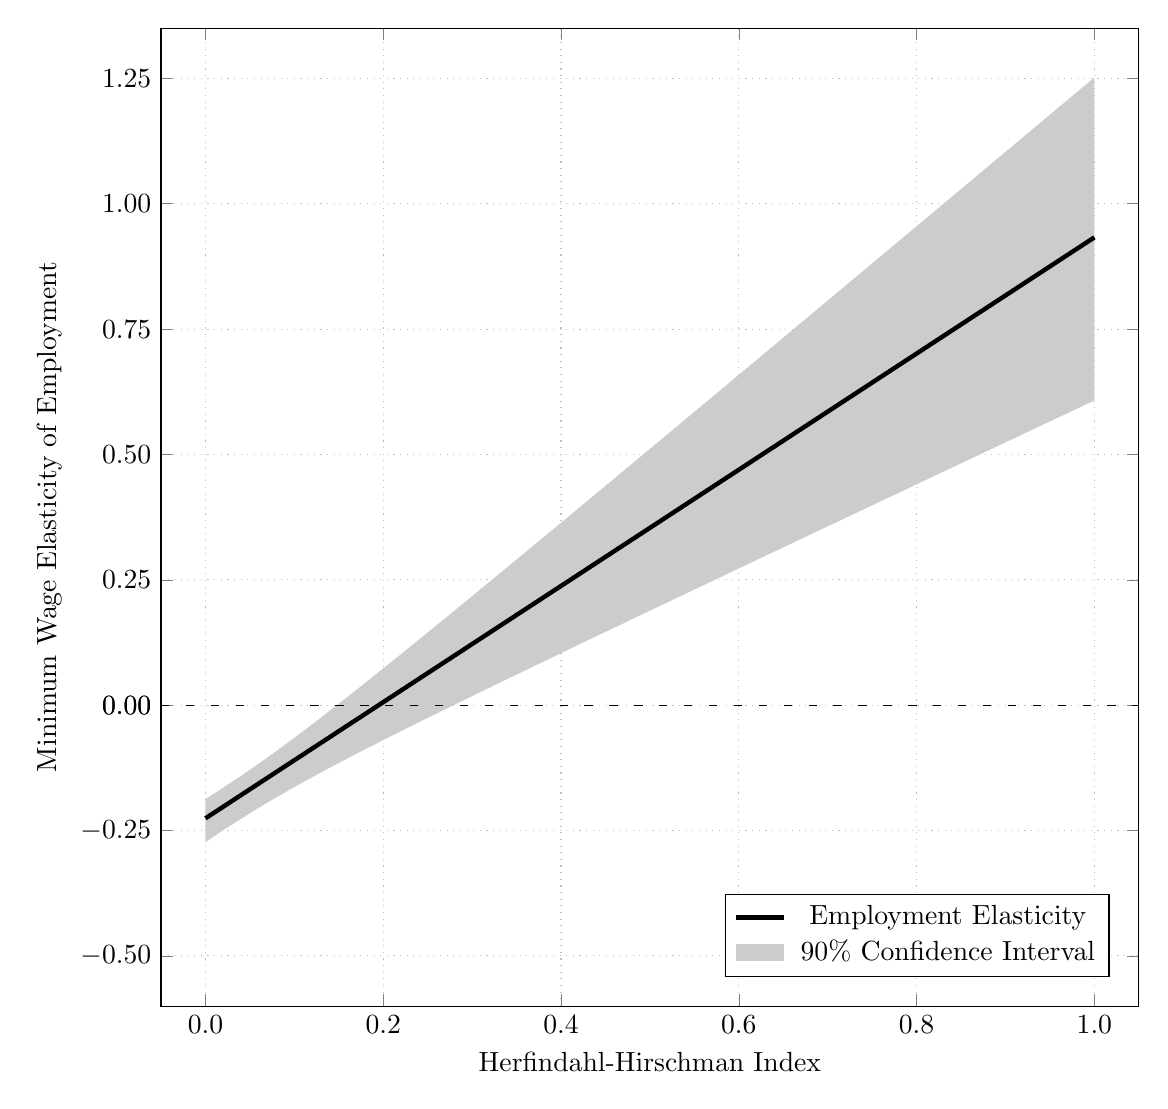
\begin{tikzpicture}
\begin{axis}[xlabel=Herfindahl-Hirschman Index, ylabel=Minimum Wage Elasticity of Employment, xmin=-0.05,xmax=1.05, ymax=1.35, ymin=-0.60, height=14cm, width=14cm, grid=major, grid style=dotted, ytick={-0.50,-0.25,0,0.25,0.50,0.75,1.00,1.25}, extra y tick style={grid=none}, extra y ticks={0}, xtick={0,0.2,0.4,0.6,0.8,1.0}, legend pos = south east, y tick label style={/pgf/number format/.cd,fixed,fixed zerofill, precision=2,/tikz/.cd}, x tick label style={/pgf/number format/.cd,fixed,fixed zerofill, precision=1,/tikz/.cd}]
\addplot[domain=0:1, color=black, solid, line width=1.6pt] { -.2256787978069273 + 1.158594926535913 * x };
%\addplot[only marks,mark=square*,mark options={fill=black}, color=black, error bar legend, error bars/.cd, y dir=both, y explicit] coordinates {  (.,.)+-(0,.) (.19678715,.00231779)+-(0,.07013807) (.39759037,.23496738)+-(0,.12909827) (.59839356,.46761695)+-(0,.1924887) (.79919678,.70026654)+-(0,.25705245) (1,.9329161)+-(0,.32208467) };
\addplot[draw=none, name path = A] coordinates {   (0,-.18693607) (.00401606,-.18250069) (.00803213,-.1780261) (.01204819,-.17351179) (.01606426,-.16895735) (.02008032,-.16436249) (.02409638,-.15972704) (.02811245,-.15505092) (.03212851,-.15033418) (.03614458,-.14557701) (.04016064,-.14077966) (.04417671,-.13594255) (.04819277,-.13106616) (.05220884,-.12615107) (.0562249,-.12119798) (.06024097,-.11620765) (.06425703,-.11118092) (.06827309,-.10611869) (.07228915,-.10102189) (.07630522,-.09589154) (.08032128,-.09072865) (.08433735,-.08553427) (.08835341,-.0803095) (.09236947,-.07505538) (.09638554,-.06977301) (.10040161,-.06446346) (.10441767,-.0591278) (.10843374,-.05376708) (.1124498,-.04838232) (.11646587,-.04297454) (.12048193,-.0375447) (.12449799,-.03209377) (.12851405,-.02662267) (.13253012,-.02113227) (.13654618,-.01562345) (.14056225,-.01009702) (.14457831,-.0045538) (.14859438,.0010055) (.15261044,.0065801) (.15662651,.01216935) (.16064256,.01777255) (.16465864,.0233891) (.16867469,.02901836) (.17269076,.0346598) (.17670682,.04031282) (.18072289,.04597695) (.18473895,.05165165) (.18875502,.05733648) (.19277108,.06303097) (.19678715,.06873473) (.20080322,.07444733) (.20481928,.08016836) (.20883535,.0858975) (.21285141,.09163437) (.21686748,.09737867) (.22088353,.10313005) (.2248996,.10888826) (.22891566,.11465296) (.23293173,.12042394) (.23694779,.12620088) (.24096386,.13198361) (.24497992,.13777183) (.24899599,.14356537) (.25301206,.14936399) (.2570281,.15516748) (.26104417,.16097568) (.26506025,.16678841) (.26907632,.1726055) (.27309236,.17842671) (.27710843,.18425201) (.2811245,.19008116) (.28514057,.19591406) (.28915662,.2017505) (.29317269,.20759045) (.29718876,.21343374) (.30120483,.21928026) (.30522087,.22512983) (.30923694,.23098245) (.31325302,.23683797) (.31726909,.24269629) (.32128513,.24855727) (.3253012,.25442091) (.32931727,.26028705) (.33333334,.26615563) (.33734939,.27202657) (.34136546,.2778998) (.34538153,.28377524) (.3493976,.28965285) (.35341364,.29553246) (.35742971,.30141413) (.36144578,.30729774) (.36546186,.31318325) (.3694779,.31907055) (.37349397,.32495964) (.37751004,.33085045) (.38152611,.33674297) (.38554215,.34263703) (.38955823,.34853271) (.3935743,.3544299) (.39759037,.36032861) (.40160644,.36622873) (.40562248,.37213022) (.40963855,.3780331) (.41365463,.38393733) (.4176707,.38984281) (.42168674,.39574954) (.42570281,.40165749) (.42971888,.40756664) (.43373495,.41347694) (.437751,.41938832) (.44176707,.42530084) (.44578314,.43121442) (.44979921,.43712905) (.45381525,.44304463) (.45783132,.44896123) (.46184739,.45487881) (.46586347,.46079731) (.46987951,.46671668) (.47389558,.47263697) (.47791165,.47855815) (.48192772,.48448017) (.48594376,.49040297) (.48995984,.49632663) (.49397591,.50225109) (.49799198,.50817627) (.50200802,.51410216) (.50602412,.52002895) (.51004016,.52595627) (.51405621,.53188437) (.51807231,.53781319) (.52208835,.5437426) (.52610439,.54967266) (.53012049,.55560344) (.53413653,.56153476) (.53815264,.5674668) (.54216868,.57339931) (.54618472,.57933247) (.55020082,.58526623) (.55421686,.59120047) (.5582329,.59713531) (.562249,.60307068) (.56626505,.60900658) (.57028115,.61494303) (.57429719,.62087989) (.57831323,.62681729) (.58232933,.63275522) (.58634537,.63869351) (.59036142,.64463228) (.59437752,.65057164) (.59839356,.65651131) (.60240966,.66245151) (.6064257,.66839206) (.61044174,.67433304) (.61445785,.68027449) (.61847389,.68621629) (.62248999,.69215852) (.62650603,.6981011) (.63052207,.70404404) (.63453817,.70998746) (.63855422,.71593112) (.64257026,.72187519) (.64658636,.72781962) (.6506024,.73376441) (.6546185,.73970956) (.65863454,.74565494) (.66265059,.75160068) (.66666669,.75754684) (.67068273,.76349324) (.67469877,.76943994) (.67871487,.77538699) (.68273091,.78133428) (.68674701,.78728199) (.69076306,.79322982) (.6947791,.799178) (.6987952,.80512655) (.70281124,.81107521) (.70682728,.81702423) (.71084338,.82297355) (.71485943,.82892305) (.71887553,.8348729) (.72289157,.84082294) (.72690761,.84677321) (.73092371,.85272378) (.73493975,.85867453) (.7389558,.86462551) (.7429719,.8705768) (.74698794,.87652826) (.75100404,.88248003) (.75502008,.88843191) (.75903612,.89438397) (.76305223,.90033638) (.76706827,.90628892) (.77108431,.91224164) (.77510041,.91819471) (.77911645,.92414784) (.78313255,.93010128) (.78714859,.93605477) (.79116464,.9420085) (.79518074,.94796252) (.79919678,.95391661) (.80321288,.95987099) (.80722892,.96582544) (.81124496,.97178012) (.81526107,.97773498) (.81927711,.98369002) (.82329315,.98964518) (.82730925,.99560058) (.83132529,1.001556) (.83534139,1.0075119) (.83935744,1.0134677) (.84337348,1.0194236) (.84738958,1.0253798) (.85140562,1.0313361) (.85542166,1.0372926) (.85943776,1.0432492) (.86345381,1.0492059) (.86746991,1.0551629) (.87148595,1.0611199) (.87550199,1.067077) (.87951809,1.0730345) (.88353413,1.0789919) (.88755018,1.0849495) (.89156628,1.0909073) (.89558232,1.0968652) (.89959842,1.1028231) (.90361446,1.1087812) (.9076305,1.1147395) (.9116466,1.120698) (.91566265,1.1266564) (.91967869,1.132615) (.92369479,1.1385738) (.92771083,1.1445327) (.93172693,1.1504917) (.93574297,1.1564507) (.93975902,1.1624099) (.94377512,1.1683693) (.94779116,1.1743287) (.9518072,1.1802882) (.9558233,1.1862479) (.95983934,1.1922077) (.96385545,1.1981676) (.96787149,1.2041276) (.97188753,1.2100875) (.97590363,1.2160478) (.97991967,1.222008) (.98393571,1.2279683) (.98795182,1.2339289) (.99196786,1.2398894) (.99598396,1.2458501) (1,1.2518108) };
\addplot[draw=none, name path = B] coordinates {   (0,-.27333948) (.00401606,-.26845872) (.00803213,-.26361716) (.01204819,-.25881535) (.01606426,-.25405365) (.02008032,-.24933235) (.02409638,-.24465168) (.02811245,-.24001165) (.03212851,-.23541225) (.03614458,-.23085329) (.04016064,-.2263345) (.04417671,-.22185548) (.04819277,-.21741574) (.05220884,-.21301466) (.0562249,-.20865162) (.06024097,-.20432581) (.06425703,-.20003641) (.06827309,-.1957825) (.07228915,-.19156316) (.07630522,-.18737738) (.08032128,-.18322413) (.08433735,-.17910236) (.08835341,-.17501101) (.09236947,-.17094898) (.09638554,-.16691521) (.10040161,-.16290861) (.10441767,-.15892813) (.10843374,-.15497272) (.1124498,-.15104133) (.11646587,-.14713298) (.12048193,-.14324668) (.12449799,-.13938147) (.12851405,-.13553645) (.13253012,-.13171069) (.13654618,-.12790339) (.14056225,-.12411366) (.14457831,-.12034076) (.14859438,-.11658391) (.15261044,-.11284238) (.15662651,-.10911548) (.16064256,-.10540256) (.16465864,-.10170295) (.16867469,-.09801609) (.17269076,-.09434137) (.17670682,-.09067827) (.18072289,-.08702625) (.18473895,-.08338482) (.18875502,-.0797535) (.19277108,-.07613187) (.19678715,-.07251947) (.20080322,-.06891591) (.20481928,-.06532082) (.20883535,-.06173381) (.21285141,-.05815456) (.21686748,-.0545827) (.22088353,-.05101796) (.2248996,-.04746002) (.22891566,-.0439086) (.23293173,-.04036342) (.23694779,-.03682425) (.24096386,-.03329081) (.24497992,-.02976291) (.24899599,-.02624029) (.25301206,-.02272277) (.2570281,-.01921015) (.26104417,-.01570221) (.26506025,-.01219879) (.26907632,-.00869972) (.27309236,-.00520485) (.27710843,-.00171398) (.2811245,.00177302) (.28514057,.00525628) (.28915662,.00873593) (.29317269,.01221213) (.29718876,.015685) (.30120483,.01915464) (.30522087,.02262115) (.30923694,.02608468) (.31325302,.02954531) (.31726909,.03300316) (.32128513,.03645827) (.3253012,.03991079) (.32931727,.04336079) (.33333334,.04680835) (.33734939,.05025353) (.34136546,.05369644) (.34538153,.05713715) (.3493976,.06057571) (.35341364,.06401218) (.35742971,.06744666) (.36144578,.0708792) (.36546186,.07430986) (.3694779,.07773866) (.37349397,.08116571) (.37751004,.08459104) (.38152611,.08801471) (.38554215,.09143673) (.38955823,.0948572) (.3935743,.09827615) (.39759037,.10169362) (.40160644,.10510964) (.40562248,.10852424) (.40963855,.1119375) (.41365463,.11534945) (.4176707,.1187601) (.42168674,.12216949) (.42570281,.12557767) (.42971888,.12898467) (.43373495,.13239053) (.437751,.13579524) (.44176707,.13919888) (.44578314,.14260146) (.44979921,.14600299) (.45381525,.1494035) (.45783132,.15280305) (.46184739,.15620163) (.46586347,.15959927) (.46987951,.16299599) (.47389558,.16639185) (.47791165,.16978683) (.48192772,.17318097) (.48594376,.17657425) (.48995984,.17996675) (.49397591,.18335848) (.49799198,.18674941) (.50200802,.19013959) (.50602412,.19352908) (.51004016,.1969178) (.51405621,.20030583) (.51807231,.20369323) (.52208835,.2070799) (.52610439,.21046592) (.53012049,.21385135) (.53413653,.21723612) (.53815264,.22062032) (.54216868,.22400387) (.54618472,.22738683) (.55020082,.23076928) (.55421686,.23415111) (.5582329,.23753241) (.562249,.24091321) (.56626505,.24429344) (.57028115,.2476732) (.57429719,.25105241) (.57831323,.25443113) (.58232933,.25780943) (.58634537,.2611872) (.59036142,.26456448) (.59437752,.26794139) (.59839356,.27131778) (.60240966,.27469382) (.6064257,.27806935) (.61044174,.28144446) (.61445785,.28481922) (.61847389,.28819352) (.62248999,.2915675) (.62650603,.29494101) (.63052207,.29831415) (.63453817,.301687) (.63855422,.3050594) (.64257026,.30843145) (.64658636,.31180319) (.6506024,.31517452) (.6546185,.31854558) (.65863454,.32191625) (.66265059,.3252866) (.66666669,.32865667) (.67068273,.33202639) (.67469877,.33539578) (.67871487,.33876494) (.68273091,.34213373) (.68674701,.34550229) (.69076306,.34887049) (.6947791,.35223842) (.6987952,.35560614) (.70281124,.3589735) (.70682728,.3623406) (.71084338,.36570749) (.71485943,.36907408) (.71887553,.37244046) (.72289157,.37580654) (.72690761,.37917235) (.73092371,.38253799) (.73493975,.38590333) (.7389558,.38926843) (.7429719,.39263335) (.74698794,.395998) (.75100404,.39936247) (.75502008,.40272668) (.75903612,.40609065) (.76305223,.40945446) (.76706827,.41281801) (.77108431,.41618139) (.77510041,.41954458) (.77911645,.4229075) (.78313255,.42627031) (.78714859,.42963287) (.79116464,.43299523) (.79518074,.43635744) (.79919678,.43971944) (.80321288,.44308129) (.80722892,.4464429) (.81124496,.44980437) (.81526107,.45316568) (.81927711,.45652676) (.82329315,.45988768) (.82730925,.46324849) (.83132529,.46660909) (.83534139,.46996957) (.83935744,.47332984) (.84337348,.47668996) (.84738958,.48004997) (.85140562,.48340976) (.85542166,.48676941) (.85943776,.49012896) (.86345381,.49348834) (.86746991,.4968476) (.87148595,.50020665) (.87550199,.50356555) (.87951809,.50692439) (.88353413,.51028305) (.88755018,.5136416) (.89156628,.51700002) (.89558232,.52035826) (.89959842,.52371645) (.90361446,.5270744) (.9076305,.53043228) (.9116466,.53379005) (.91566265,.5371477) (.91967869,.54050517) (.92369479,.54386258) (.92771083,.54721987) (.93172693,.55057704) (.93574297,.55393404) (.93975902,.55729097) (.94377512,.56064785) (.94779116,.56400448) (.9518072,.56736106) (.9558233,.57071757) (.95983934,.57407397) (.96385545,.57743025) (.96787149,.58078641) (.97188753,.58414245) (.97590363,.58749849) (.97991967,.59085429) (.98393571,.59421003) (.98795182,.59756577) (.99196786,.60092133) (.99598396,.60427684) (1,.60763216) };
\addplot[color=gray!40!white] fill between[of=A and B];
\addplot[loosely dashed] coordinates {(-0.05,0) (1.05,0)};
\legend{~Employment Elasticity,,,~90\% Confidence Interval,}
\end{axis}
\end{tikzpicture}
}
\floatfoot{ \footnotesize \textsc{Note. ---} The figure illustrates estimated employment elasticities with respect to changes in sectoral minimum wages at the establishment level. Estimates stem from fixed effects regressions of log establishment-level employment (of regular full-time workers) on log sectoral minimum wages as well as their interaction effect with labor market concentration (measured as average HHI). The thick line reports point estimates of employment elasticities across different levels of concentration. The grey shade represents 90 percent confidence intervals. Sources: IEB $\plus$ BHP $\plus$ IAB Establishment Panel, 1999-2017.}
\end{figure}

\paragraph{Sensitivity and Heterogeneity.} I perform multiple checks to examine the sensitivity and heterogeneity of the estimated employment effects. As the establishment-weighted distribution of HHI is not uniform, the identification of the linear interaction effect may not reflect all parts of the HHI range equally. To ascertain that the positive HHI gradient is not just a result of the linearity assumption, I construct categorial interaction effects between minimum wage levels and indicator variables that separate low- from high-HHI labor markets. Table \ref{tab:E4} shows main and interactions effects for divisions of the HHI range into two, three, four and five domains.\footnote{I construct the domains such that the E.U.\ antitrust thresholds for HHI are respected.} Across these specifications, the estimates exhibit the same qualitative pattern as before: negative employment responses in unconcentrated markets that weaken for higher HHI domains and, ultimately, become positive. In this respect, Figure \ref{fig:3} illustrates the estimated pattern of elasticities for a categorization into five HHI domains.

\begin{figure}[!ht]
\centering
\caption{Minimum Wage Elasticity of Employment by HHI Categories}
\label{fig:3}
\scalebox{0.80}{
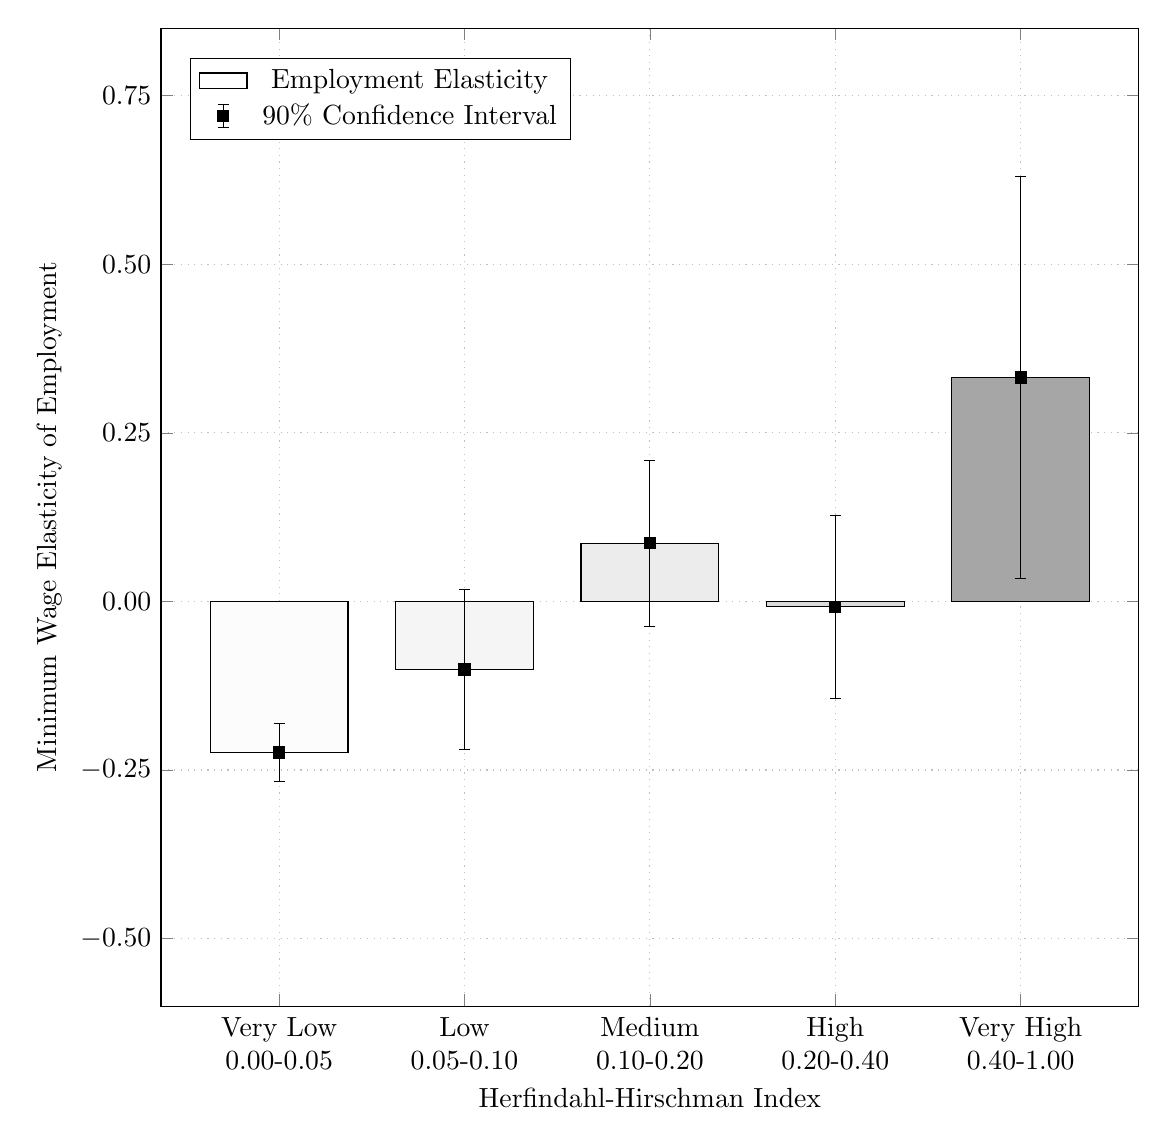
\begin{tikzpicture}
\begin{axis}[xlabel=Herfindahl-Hirschman Index, ylabel=Minimum Wage Elasticity of Employment, ymax=0.85, ymin=-0.60, height=14cm, width=14cm, grid=major, grid style=dotted, bar width=1.75cm,enlarge x limits={abs=1.5cm}, xtick={1,2,3,4,5},xticklabels={\shortstack{Very Low\vphantom{/}\\ 0.00-0.05}, \shortstack{Low\vphantom{/}\\ 0.05-0.10}, \shortstack{Medium\vphantom{/}\\ 0.10-0.20}, \shortstack{High\vphantom{/}\\ 0.20-0.40}, \shortstack{Very High\vphantom{/}\\ 0.40-1.00} }, ytick={-0.50,-0.25,0,0.25,0.50,0.75}, legend pos = north west, y tick label style={/pgf/number format/.cd,fixed,fixed zerofill, precision=2,/tikz/.cd}]
\addplot[ybar, area legend, color=black, fill=white] coordinates {(1,0)}; %only for legend with white bar entry
\addplot[ybar, area legend, color=black, fill=gray!2.5!white] coordinates {(1,-.2239164)};
\addplot[ybar, area legend, color=black, fill=gray!7.5!white] coordinates {(2,-.10105073)};
\addplot[ybar, area legend, color=black, fill=gray!15!white] coordinates {(3,.08641531)};
\addplot[ybar, area legend, color=black, fill=gray!30!white] coordinates {(4,-.00809857)};
\addplot[ybar, area legend, color=black, fill=gray!70!white] coordinates {(5,.33204827)};
\addplot[only marks,mark=square*, color=black, error bar legend, error bars/.cd, y dir=both, y explicit] coordinates { (1,-.2239164)+-(0,.04268356) (2,-.10105073)+-(0,.11892477) (3,.08641531)+-(0,.12315473) (4,-.00809857)+-(0,.13613619) (5,.33204827)+-(0,.29746291) };
\legend{~Employment Elasticity,,,,,,~90\% Confidence Interval}
\end{axis}
\end{tikzpicture}
}
\floatfoot{ \footnotesize \textsc{Note. ---} The figure illustrates estimated employment elasticities with respect to changes in sectoral minimum wages at the establishment level. Estimates stem from fixed effects regressions of log establishment-level employment (of regular full-time workers) on log sectoral minimum wages as well as their categorial interaction effects of labor market concentration (measured as average HHI). The bars illustrate point estimates for establishments in labor markets with different levels of concentration. Each point estimates features a 90 percent confidence interval. Sources: IEB $\plus$ BHP $\plus$ IAB Establishment Panel, 1999-2017.}
\end{figure}

The empirical results also withstand further scrutiny. Figure \ref{fig:4} contrasts the baseline elasticities with those from alternative versions of Equation (\ref{eq:4}), evaluated at the lower and upper end of the HHI range. In more detail, the appendix illustrates the underlying estimates for alternative specifications (Table \ref{tab:E5}), labor market definitions (Table \ref{tab:E6}), and concentration measures (Table \ref{tab:E7}) as well as separate regressions by territories (Table \ref{tab:E8}) and labor outcomes (Table \ref{tab:E9}). In general, the results are robust to various modifications of the baseline equation, thus lending further support to the monopsony argument.

In line with the insignificant correlation between HHI and sectoral minimum wage levels (see Table \ref{tab:E1}), the use of time-variant HHIs or a predetermined HHI per establishment (as an alternative to establishment-specific HHI averages) does not lead to marked changes in the elasticity estimates.\footnote{As a more rigorous alternative to establishment-specific HHI averages, predetermined HHIs eliminate any reverse causality between employment and HHI as well as the confounding impact of non-local shocks on HHI values. As a drawback, however, predetermined HHIs provide a less representative picture of the underlying labor market concentration over the period of study. Specifically, I use the corresponding HHI value of the same labor market, but in the year before the firm was first subject to minimum wage legislation in the period under study. For lack of information on 1998, I resort to the 1999 HHI value if needed.} Likewise, the inclusion of sector-specific linear time trends is not pivotal. Due to the logarithmic transformation, the identification of the baseline elasticities solely stems from modifications of minimum wage levels. Hence, variation from the introduction of a sectoral minimum wage does not enter the regression. Even in the absence of a minimum wage regulation, the availability of unemployment benefits or quasi-fixed cost of labor supply define a lower wage ceiling, a so-called ``implicit minimum wage''. Hence, to capture full variation in minimum wage legislation, I assign operating firms an implicit minimum wage in the year preceding the minimum wage introduction, proxied by the fifth percentile of the hourly wage distribution.\footnote{I construct hourly wages by dividing weekly earnings of full-time workers by 40 working hours per week.} In the augmented regression, the interaction effect with HHI turns out to be positive yet again while the main effect remains negative.

%Moreover, the implementation of a first-difference estimation yields similar results, albeit with smaller absolute magnitude.

Further, the observed pattern of elasticities is not sensitive to broader or narrower definitions of labor markets. Whereas 5-digit NACE industries experience similar interaction effects, 3-digit NACE industries or 3-digit NUTS regions exhibit less positive but still significant interaction effects. The latter finding also holds true when constructing the HHI based on new hires instead of the stock of employment. Moreover, the results remain unchanged for alternative concentration indices: the Rosenbluth Index, the 1-Subject Concentration Ratio, the Inverse Number of Subjects, and the Exponential Index deliver robust estimates.

\begin{figure}[!ht]
\centering
\caption{Sensitivity and Heterogeneity of Employment Effects}
\label{fig:4}
\scalebox{0.80}{
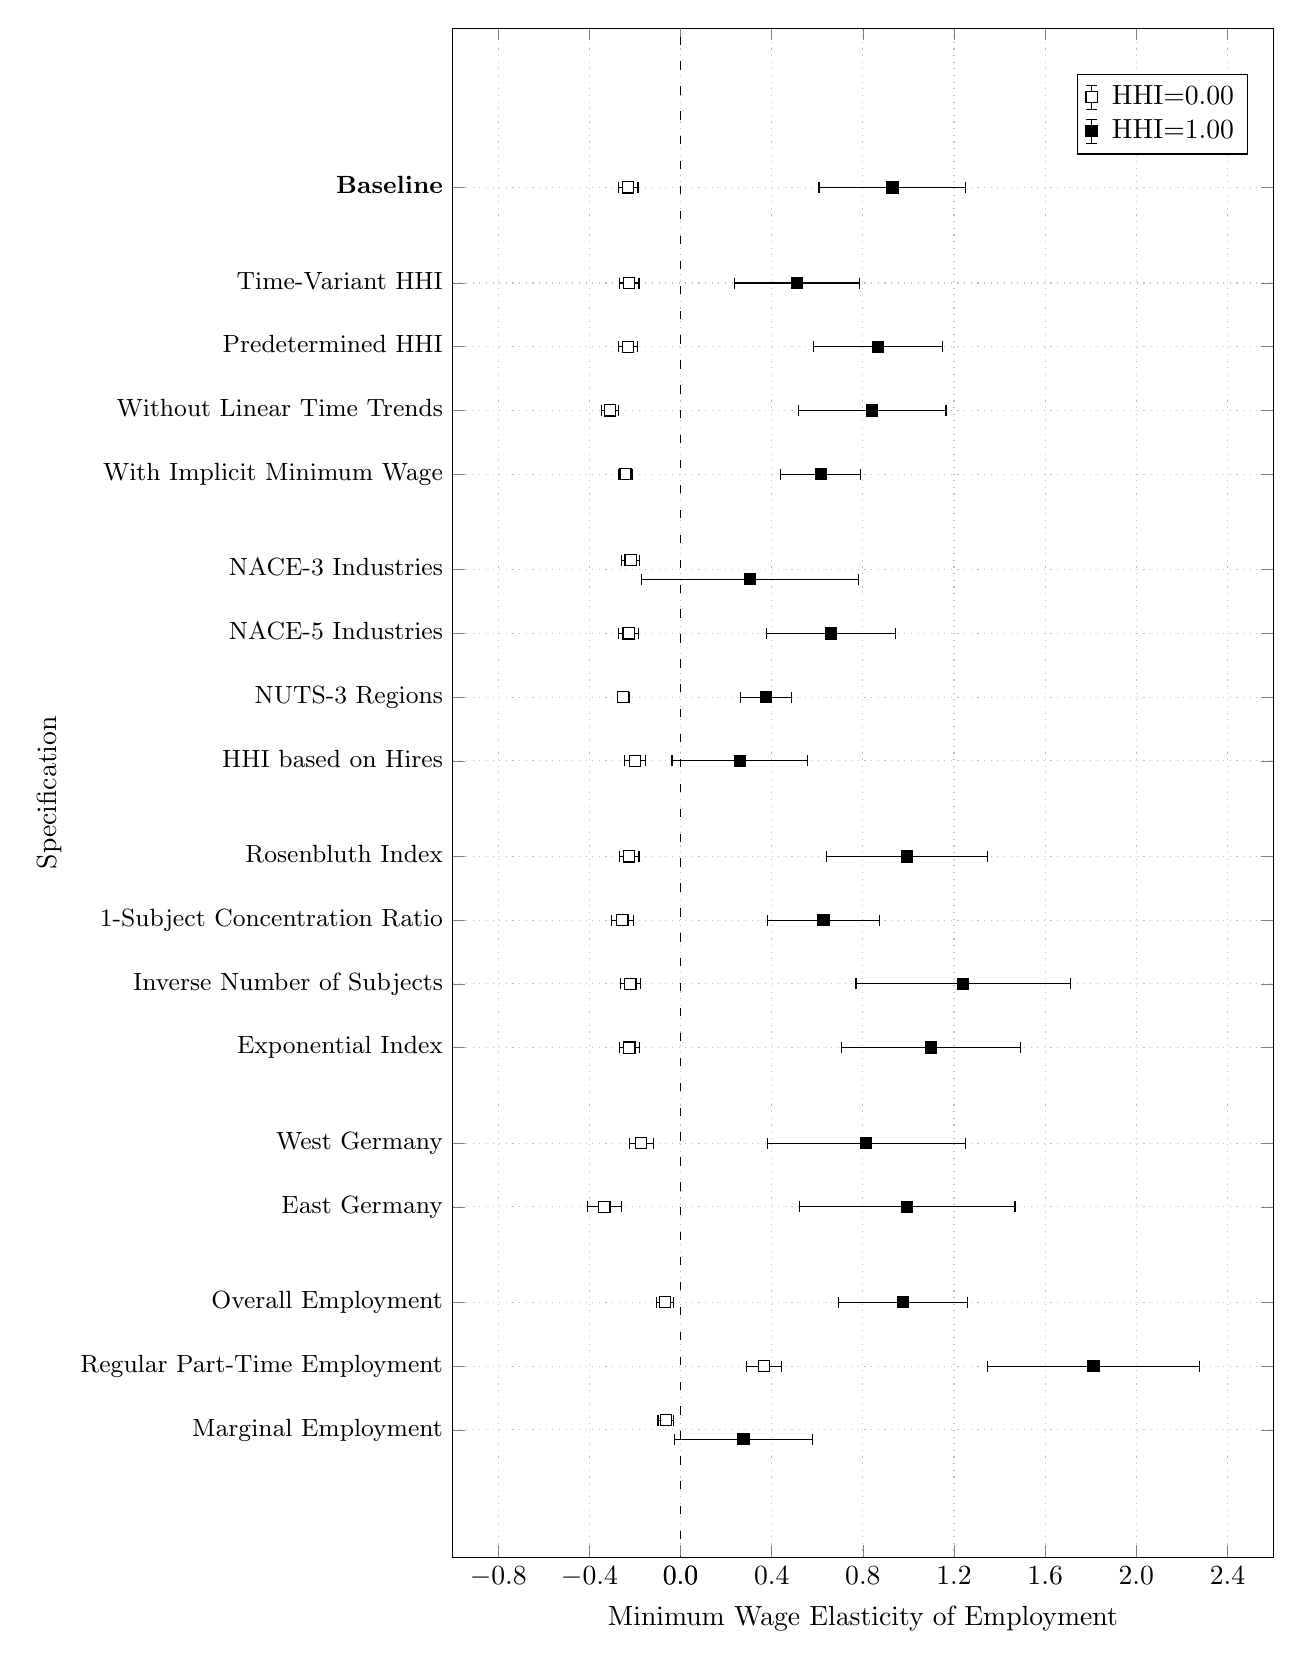
\begin{tikzpicture}
\begin{axis}[xlabel=Minimum Wage Elasticity of Employment, ylabel=Specification, height=21cm, width=12cm, grid=major, grid style=dotted, xmin=-1, xmax=2.6, ymin=-1, ymax=23, xtick={-0.8,-0.4,0,0.4,0.8,1.2,1.6,2.0,2.4}, extra x tick style={grid=none}, extra x ticks={0}, legend pos= north east, x tick label style={/pgf/number format/.cd,fixed,fixed zerofill, precision=1,/tikz/.cd},y tick label style = {font=\small}, ytick={1,2,3,4.5,5.5,7,8,9,10,11.5,12.5,13.5,14.5,16,17,18,19,20.5}, yticklabels={{Marginal Employment\vphantom{/}},{Regular Part-Time Employment\vphantom{/}},{Overall Employment\vphantom{/}},{East Germany\vphantom{/}},{West Germany\vphantom{/}},{Exponential Index\vphantom{/}},{Inverse Number of Subjects\vphantom{/}},{1-Subject Concentration Ratio\vphantom{/}},{Rosenbluth Index\vphantom{/}},{HHI based on Hires\vphantom{/}},{NUTS-3 Regions\vphantom{/}},{NACE-5 Industries\vphantom{/}},{NACE-3 Industries\vphantom{/}},{With Implicit Minimum Wage\vphantom{/}},{Without Linear Time Trends\vphantom{/}},{Predetermined HHI\vphantom{/}},{Time-Variant HHI\vphantom{/}},{\textbf{Baseline}\vphantom{/}},}]
\addplot[only marks,mark=square*,mark options={fill=white},color=black, error bar legend, error bars/.cd, x dir=both, x explicit] coordinates {  (-.06443085,1.15)+-(.03477307,0) (.36485443,2)+-(.07658616,0) (-.06763344,3)+-(.03702141,0) (-.33396047,4.5)+-(.07429746,0) (-.17244625,5.5)+-(.05349021,0) (-.22433941,7)+-(.04263239,0) (-.21997508,8)+-(.04231378,0) (-.25501865,9)+-(.04682845,0) (-.22524369,10)+-(.04268622,0) (-.20074998,11.5)+-(.04608591,0) (-.25122949,12.5)+-(.0264743,0) (-.22832182,13.5)+-(.04368311,0) (-.21943106,14.65)+-(.04055502,0) (-.24163921,16)+-(.03159304,0) (-.30838054,17)+-(.03761837,0) (-.23025456,18)+-(.04304543,0) (-.22520792,19)+-(.04293159,0) (-.23013777,20.5)+-(.04320171,0) };
\addplot[only marks,mark=square*, color=black, error bar legend, error bars/.cd, x dir=both, x explicit] coordinates {  (.27642578,0.85)+-(.30218935,0) (1.8120064,2)+-(.46517229,0) (.97641993,3)+-(.284491,0) (.99409705,4.5)+-(.47343367,0) (.81470257,5.5)+-(.43472746,0) (1.09858,7)+-(.39376432,0) (1.2404234,8)+-(.47078007,0) (.62707651,9)+-(.24754101,0) (.99334687,10)+-(.35453528,0) (.2607609,11.5)+-(.29818866,0) (.37650853,12.5)+-(.11160824,0) (.65957874,13.5)+-(.28410578,0) (.30300832,14.35)+-(.47604236,0) (.61483538,16)+-(.17571783,0) (.84088689,17)+-(.32393104,0) (.86591589,18)+-(.28194118,0) (.51068521,19)+-(.27387875,0) (.92972153,20.5)+-(.32208937,0) };
\addplot[loosely dashed] coordinates {(0,-1.5) (0,23.5)};
\legend{~HHI=0.00~,~HHI=1.00~}
\end{axis}
\end{tikzpicture}
}  \vspace*{-0.25cm}
\floatfoot{ \footnotesize \textsc{Note. ---} The figure illustrates minimum wage elasticities of employment at polar values of labor market concentration for a variety of specifications. Hollow squares refer to point estimates for zero HHI whereas solid squares represent estimates that relate to HHI=1. Each point estimate features a 90 percent confidence interval. The baseline estimation regresses establishment-level employment of regular full-time workers on sectoral minimum wages, an interaction effect with the establishment-level average of employment-based HHI per labor market (defined as NACE-4-industry-by-commuting-zone combination), a set of control variables (including log overall employment per sector-by-territory combination, the sectoral share of establishments subject to a collective bargaining agreement, and sector-specific linear time trends) as well as on establishment and year-by-commuting-zone fixed effects. HHI = Herfindahl-Hirschman Index. NACE-X = X-Digit Statistical Nomenclature of Economic Activities in the European Community. NUTS-X = X-Digit Statistical Nomenclature of Territorial Units. Sources: IEB $\plus$ BHP $\plus$ IAB Establishment Panel, 1999-2017.}
\end{figure}

Despite structural differences, establishments in both West and East Germany equally feature minimum wage elasticities of employment that are negative in competitive but positive in monopsonistic labor markets. For labor markets with zero HHI, employment effects are more negative in East Germany where the bite is also larger. There is no such difference for highly concentrated labor markets. Importantly, the findings are not restricted to the employment of regular full-time workers but also hold for overall employment per firm. Interestingly, regular part-time workers exhibit significant job growth both in slightly concentrated and, to a larger extent, in highly concentrated labor markets. Given that the employment of regular full-time workers shows a fairly strong decline in slightly concentrated labor markets, an obvious explanation for the large increase in regular-part time employment at zero HHI is a reduction in individual working hours that has transformed some of the regular full-time workers into regular part-time workers. Moreover, by virtue of higher sectoral minimum wage levels, the monthly income of marginal part-time workers increasingly exceeds the threshold above which job contracts automatically turn into regular part-time employment.\footnote{Marginal employment involves reduced social security contributions for work contracts below a legally defined income threshold. Since April 1, 1999, the monthly salary must not exceed 325 Euro. On April 1, 2003 and January 1, 2013, the threshold was lifted to 400 and 450 Euro per month, respectively.} This mechanism is supposed to be more pronounced in concentrated markets where wage increases tend to be higher. Accordingly, for HHI=1, the minimum wage elasticity for marginal employment features the smallest positive value among the labor outcomes.


\paragraph{Nonlinearities.} In monopsonistic labor markets, the minimum wage effect on employment differs between three regimes of bindingness: zero (or small) effects in the unconstrained regime (i.e., the minimum wage does not bite), positive effects in the supply-determined regime (i.e., the minimum wage counteracts monopsonistic exploitation), and negative effects in the demand-determined regime (i.e., firms lay off the least productive workers). To check whether reported minimum wage effects on employment obscure heterogeneity by the underlying bite of the sectoral minimum wage, I re-run the baseline regression on a full set of interaction terms between log sectoral minimum wage, labor market concentration (measured as average HHI), and indicator variables for five quintiles of bindingness of the sectoral minimum wage in a firm (measured as average Kaitz Index, see Table \ref{tab:E10}).\footnote{The Kaitz Index is calculated as the ratio of the sectoral minimum wage to the median hourly wage rate of regular full-time workers within an establishment. For lack of IEB information on individual working hours, I construct hourly wage rates by dividing weekly earnings of regular full-time workers by 40 working hours per week. I assign each firm one of the following five quintile groups given their average Kaitz Index across available years: 0-0.68 (first group), 0.68-0.79 (second group), 0.79-0.92 (third group), 0.92-1.15 (fourth group), and higher than 1.15 (fifth group).}

Figure \ref{fig:5} visualizes the resulting minimum wage elasticities of employment by quintile of bindingness, separately for markets with HHI=0 and HHI=1. As expected, the negative employment effect in zero-HHI markets becomes more negative when the bite is large: in the fifth quintile of the Kaitz Index, the minimum wage elasticity of employment is about twice as negative as in the first quintile (Panel a). In line with monopsony theory, the minimum wage elasticity of employment in highly concentrated labor markets is a non-linear function of the underlying bite (Panel b). At first, the positive employment effect grows with the bite, counteracting monopsonistic exploitation along the labor supply curve. But, beginning with the fourth quintile (i.e., when the minimum wage is set close to the median wage of the firm), the positive minimum wage effect falls rapidly. Although the minimum wage elasticity of employment in the fifth quintile of bindingness is not significantly different from zero, it is significantly smaller than the values in the first, second, and third quintile. Overall, the quadratic relationship implies that, given a higher bindingness, firms' adjustment increasingly takes place along the negatively sloped labor demand curve since minimum wages start to exceed workers' marginal productivity.

\afterpage{
\begin{landscape}

\vspace*{\fill}

\begin{figure}[!ht]
\centering
\caption{Minimum Wage Elasticity of Employment by Bindingness}
\label{fig:5}
\vspace*{0.5cm}
\begin{subfigure}{0.475\textwidth}
\centering
\caption{Evaluated at HHI=0}
\scalebox{0.85}{
\begin{tikzpicture}
\begin{axis}[xlabel=Quintile of Kaitz Index, ylabel=Minimum Wage Elasticity of Employment, ymax=2.5, ymin=-2.5, height=12cm, width=14cm, grid=major, grid style=dotted, bar width=1.75cm,enlarge x limits={abs=1.5cm}, xtick={1,2,3,4,5},xticklabels={First, Second, Third, Fourth, Fifth}, ytick={-2,-1,0,1,2}, legend pos = south west, y tick label style={/pgf/number format/.cd,fixed,fixed zerofill, precision=0,/tikz/.cd}]
%\addplot[ybar, area legend, color=black, fill=white] coordinates {(1,0)}; %only for legend with white bar entry
\addplot[ybar, area legend, color=black, fill=white] coordinates {(1,-.23978776)};
\addplot[ybar, area legend, color=black, fill=white] coordinates {(2,-.14515065)};
\addplot[ybar, area legend, color=black, fill=white] coordinates {(3,-.1207806)};
\addplot[ybar, area legend, color=black, fill=white] coordinates {(4,-.29994184)};
\addplot[ybar, area legend, color=black, fill=white] coordinates {(5,-.54131156)};
\addplot[only marks,mark=square*, color=black, error bar legend, error bars/.cd, y dir=both, y explicit] coordinates {   (1,-.23978776)+-(0,.05645117) (2,-.14515065)+-(0,.04991314) (3,-.1207806)+-(0,.05228676) (4,-.29994184)+-(0,.06898138) (5,-.54131156)+-(0,.10970056) };
\legend{~Employment Elasticity,,,,,~90\% Confidence Interval}
\end{axis}
\end{tikzpicture}
}
\end{subfigure}
\hfill
\begin{subfigure}{0.475\textwidth}
\centering
\caption{Evaluated at HHI=1}
\scalebox{0.85}{
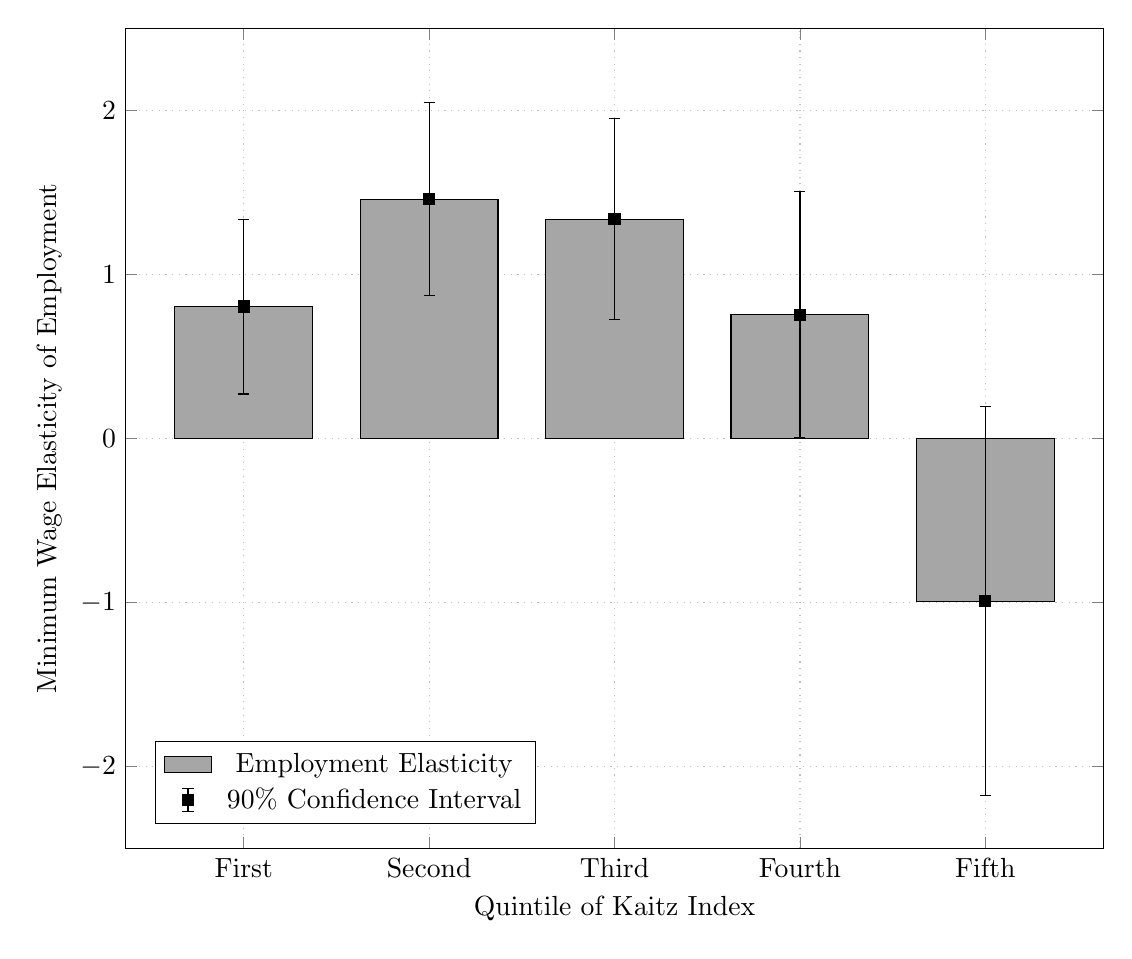
\begin{tikzpicture}
\begin{axis}[xlabel=Quintile of Kaitz Index, ylabel=Minimum Wage Elasticity of Employment, ymax=2.5, ymin=-2.5, height=12cm, width=14cm, grid=major, grid style=dotted, bar width=1.75cm,enlarge x limits={abs=1.5cm}, xtick={1,2,3,4,5},xticklabels={First, Second, Third, Fourth, Fifth}, ytick={-2,-1,0,1,2}, legend pos = south west, y tick label style={/pgf/number format/.cd,fixed,fixed zerofill, precision=0,/tikz/.cd}]
%\addplot[ybar, area legend, color=black, fill=white] coordinates {(1,0)}; %only for legend with white bar entry
\addplot[ybar, area legend, color=black, fill=gray!70!white] coordinates {(1,.80347413)};
\addplot[ybar, area legend, color=black, fill=gray!70!white] coordinates {(2,1.4581449)};
\addplot[ybar, area legend, color=black, fill=gray!70!white] coordinates {(3,1.3365678)};
\addplot[ybar, area legend, color=black, fill=gray!70!white] coordinates {(4,.75352061)};
\addplot[ybar, area legend, color=black, fill=gray!70!white] coordinates {(5,-.99180871)};
\addplot[only marks,mark=square*, color=black, error bar legend, error bars/.cd, y dir=both, y explicit] coordinates {  (1,.80347413)+-(0,.5327996) (2,1.4581449)+-(0,.58914185) (3,1.3365678)+-(0,.61189455) (4,.75352061)+-(0,.74891919) (5,-.99180871)+-(0,1.1838012) };
\legend{~Employment Elasticity,,,,,~90\% Confidence Interval}
\end{axis}
\end{tikzpicture}
}
\end{subfigure}
\floatfoot{ \footnotesize \textsc{Note. ---} The figures display estimated minimum wage elasticities of employment by quintiles of the underlying Kaitz Index. Estimates stem from fixed effects regressions of log establishment-level employment (of regular full-time workers) on a full set of interaction terms between log sectoral minimum wages, labor market concentration (measured as average HHI), and five quintile groups of minimum wage bindingness (measured as average Kaitz Index). The Kaitz Index is calculated as the ratio of the sectoral minimum wage to the median hourly wage rate of regular full-time workers within an establishment. The bars illustrate point estimates for different quintiles of the Kaitz Index at the polar values of the HHI distribution. Each point estimates features a 90 percent confidence interval. Sources: IEB $\plus$ BHP $\plus$ IAB Establishment Panel, 1999-2017.}
\end{figure}


\vspace*{\fill}

\end{landscape}
}

\paragraph{Causal Interpretation.} The previous analysis suggests that minimum wage elasticities are a function of labor market concentration. However, it is unclear whether labor market concentration causally determines minimum wage responses or just constitutes a proxy for an omitted variable that is the factual moderator of the minimum wage effect on employment. Nevertheless, in the latter case, labor market concentration would still provide correlative information on the true moderator and, thus, can guide policy makers to assess the impact of higher minimum wages \citep{AzarEtAl2019a}. Next, I scrutinize two candidates for such an omitted variable bias: product market concentration and productivity.

As mentioned in Section \ref{sec:6}, product market concentration might inadvertently enter industry-based measures of local labor market concentration. If labor market concentration was not the causal moderator of the minimum wage effects, firms would - absent any monopsony power - face a horizontally sloped labor supply curve to the single firm. Thus, the bite of minimum wages should not depend on or, when monopolists share parts of their rents with their workforce, decrease with product market concentration. Incompatible with both hypotheses, the above earnings regressions feature a positive interaction effect with HHI, supporting the notion that it is monopsony power that causally moderates the minimum wage effects. As an additional check, Column (1) in Table \ref{tab:6} shows that the employment regressions are robust to the exclusion of service sectors for which product markets are susceptible to overlap with local labor markets.


\begin{table}[!ht]
\centering
%\resizebox{\textwidth}{!}{
\scalebox{0.90}{
\begin{threeparttable}
\caption{Alternative Moderators and Establishment Closures}
\label{tab:6}
\begin{tabular}{|C{4cm}|C{3.75cm}C{3.75cm}C{3.75cm}|} \hline \hline
\multirow{4}{*}{\diagbox[height=4.4175\line, innerwidth=4cm]{Regressor}{\shortstack{ \\ \hspace{0.1cm}Dependent \\ \hspace{0.1cm}Variable }}} & \multirow{4.4}{*}{\shortstack{(1) \\ Log \\ Regular FT\vphantom{/} \\ Employment }} & \multirow{4.4}{*}{\shortstack{(2) \\ Log \\ Regular FT\vphantom{/} \\ Employment }} & \multirow{4.4}{*}{\shortstack{(3) \\ Establishment\vphantom{/} \\ Closure\vphantom{/} }}  \\
&&&      \\
&&&      \\
&&&      \\[0.2cm] \hline
\multirow{2.4}{*}{Log Minimum Wage} &  \multirow{2.4}{*}{\shortstack{\hphantom{***}-0.087***\hphantom{-} \\ (0.027)}}  & \multirow{2.4}{*}{\shortstack{\hphantom{***}-0.167***\hphantom{-} \\ (0.023)}} & \multirow{2.4}{*}{\shortstack{\hphantom{***}0.133*** \\ (0.013)}}     \\
&&&  \\
\multirow{2.4}{*}{\shortstack{Log Minimum Wage \\ $\times$ $\overline{\text{HHI}}$}} &  \multirow{2.4}{*}{\shortstack{\hphantom{***}1.666*** \\ (0.236)}}  & \multirow{2.4}{*}{\shortstack{\hphantom{***}1.188*** \\ (0.203)}} & \multirow{2.4}{*}{\shortstack{0.001 \\ (0.070)}}     \\
&&&  \\
\multirow{2.4}{*}{\shortstack{Log Minimum Wage \\ $\times$ Log $\overline{\text{AKM}}$}} &  \multirow{2.4}{*}{}  & \multirow{2.4}{*}{\shortstack{\hphantom{***}0.605*** \\ (0.081)}} & \multirow{2.4}{*}{}     \\
&&&  \\[0.2cm] \hdashline
&&& \\[-0.2cm]
Control Variables  & Yes & Yes  & Yes   \\
\multirow{2.4}{*}{\shortstack{Fixed \\ Effects}}  & \multirow{2.4}{*}{\shortstack{Establishment \\ Year $\times$ CZ}} & \multirow{2.4}{*}{\shortstack{Establishment \\ Year $\times$ CZ}} & \multirow{2.4}{*}{\shortstack{Establishment \\ Year $\times$ CZ}}  \\
&&&  \\
\multirow{3.4}{*}{\shortstack{Labor Market \\ Definition \\ (Object)}}  & \multirow{3.4}{*}{\shortstack{NACE-4 \\ $\times$ CZ \\ (Employment)}} & \multirow{3.4}{*}{\shortstack{NACE-4 \\ $\times$ CZ \\ (Employment)}} & \multirow{3.4}{*}{\shortstack{NACE-4 \\ $\times$ CZ \\ (Employment)}} \\
&&& \\
&&& \\[0.2cm] \hdashline
&&& \\[-0.4cm]
\multirow{2.4}{*}{Sample}  & \multirow{2.4}{*}{\shortstack{Without\vphantom{/} \\ Services}} & \multirow{2.4}{*}{Overall} & \multirow{2.4}{*}{\shortstack{Regular FT\vphantom{/} \\ Employment $>0$ }}  \\
&&& \\[0.2cm] \hdashline
&&& \\[-0.2cm]
Observations &  2,135,562    & 2,585,412    & 2,700,155       \\[0.2cm]
Adjusted R$^2$ &  0.860    & 0.872    &   0.156         \\[0.2cm] \hline \hline
\end{tabular}
\begin{tablenotes}
\item \footnotesize \textsc{Note. ---} The table displays fixed effects regressions of log establishment-level employment (of regular full-time workers) and an indicator for establishment closure on log sectoral minimum wages as well as their interaction effect with labor market concentration (measured as average HHI). The set of control variables includes log overall employment per sector-by-territory combination, the sectoral share of establishments subject to a collective bargaining agreement, and sector-specific linear time trends. Overall employment is defined as the sum of regular full-time workers, regular part-time workers, and workers in marginal employment. Standard errors (in parentheses) are clustered at the labor-market level. AKM = AKM Establishment Fixed Effekt. CZ = Commuting Zone. HHI = Herfindahl-Hirschman Index. NACE-4 = 4-Digit Statistical Nomenclature of Economic Activities in the European Community. FT = Full-Time. * = p$<$0.10. ** = p$<$0.05. *** = p$<$0.01. Sources: IEB $\plus$ BHP $\plus$ IAB Establishment Panel, 1999-2017.
\end{tablenotes}
\end{threeparttable}
}
\end{table}

In general, higher minimum wages will make less productive firms reduce employment more strongly than highly productive firms. For instance, the fact that labor market concentration is usually higher in rural areas, where firms also tend to be less productive, may result in a downward-biased interaction term for HHI \citep{AzarEtAl2019a}. To rule out such an omitted variable bias, I augment the baseline specification with an additional interaction effect between log minimum wage levels and firm productivity. I approximate productivity by establishment fixed effects from log-linear wage regressions in the tradition of Abowd, Kramarz, and Margolis (\citeyear{AbowdEtAl1999}, hereafter `AKM'). These AKM effects reflect a relative wage premium paid to all workers within an establishment, conditional on time-variant characteristics and individual fixed effects. Specifically, I retrieve AKM establishment fixed effects for log daily wages of regular full-time workers from \citet{BellmannEtAl2020}. In Column (2) of Table \ref{tab:6}, the AKM interaction effect turns out to be positive: an increase in firm productivity by 1 percent raises the minimum wage elasticity of employment by 0.00605. Hence, an establishment with zero HHI but a wage premium of 27.6 (=0.167/0.00605) percent will not adjust employment. Despite the moderating impact of productivity, the interaction effect with HHI remains unchanged, thus lending further credence to the monopsony argument.

\paragraph{Establishment Closures.} From a theoretical point of view, minimum wages do not only make employers adjust employment but, equally important, can cause establishments to close \citep{Williamson1968}. Apart from efficiency wage considerations, higher minimum wages are supposed to lower profits of treated firms. As a consequence, some of these firms are forced to quit the market. Following standard practice, I identify a closures for the last year in which an establishment appears in the data (e.g., \citealp{FacklerEtAl2013}). Thus, in the BHP, a closure occurs when an establishment for the last time reports employment of workers subject to social security contributions.\footnote{I use of the BHP wave from 2018 to separate factual from artificial closures at the current edge of 2017.} Prior to minimum wage legislation, the probability of closure in the relevant sectors is 6.6 percent. After treatment, this probability climbs to 9.0 percent. Column (3) of Table \ref{tab:6} displays the results from a linear probability model where the binary outcome of establishment closure is regressed on the covariates from Equation (\ref{eq:4}). The main effect is significantly positive: an increase in the minimum wage by 1 percent raises the probability of closure by 0.13 percentage points in unconcentrated labor markets. In contrast, the interaction term with HHI is not significantly different from zero. To compare market forms, however, it is necessary to normalize the coefficients by the underlying minimum wage elasticity of earnings (see Column (4) in Table \ref{tab:4}): an effective wage increase by 1 percent will raise the probability of establishment closure by 1.9 (=0.133/0.070) percentage points in unconcentrated labor markets but only by 0.4 (=(0.133+0.002)/(0.070+0.260)) percentage points in highly concentrated markets. A natural explanation for this difference are oligopsonistic rents on which firms in concentrated markets can draw to a greater extent than firms in competitive markets where profits tend to be smaller. My finding that higher sectoral minimum wages make firms exit the market complements analogous evidence on the introduction of the 2015 nation-wide minimum wage in Germany \citep{DustmannEtAl2021}.






\section{Discussion}
\label{sec:8}

In the past, many studies have attributed the absence of negative minimum wage effects on employment in Germany to the existence of monopsony power (e.g., \citealp{Moeller2012}; \citealp{Frings2013}; \citealp{CaliendoEtAl2018}). So far, however, the monopsony argument has been put forward solely on the basis of theoretical considerations rather than empirical evidence. My results provide direct empirical support to this line of argument by demonstrating that labor market concentration, the classical source for monopsony power, modulates the effect of higher minimum wages on employment. While, in line with perfect competition, minimum wages significantly reduce employment in slightly concentrated labor markets, I report zero and positive effects for moderately and highly concentrated labor markets in which firms enjoy wage-setting power. Against the backdrop of monopsony theory, the results are consistent with a non-monotonous relationship between minimum wage bindingness and employment. The positive employment effect in monopsonistic labor markets implies that wage floors were, on average, not raised well beyond market-clearing levels. In the German case, this condition is plausibly met as sectoral minimum wages stem from collective bargaining agreements that necessitate approval from the respective employer association.



In light of my results, an adequate empirical design should take into account that minimum wage effects depend on the degree of monopsony power in the labor market. However, minimum wage studies generally pool information across different labor markets and, thus, might conceal heterogeneity by market form. If so, these studies arrive at close-to-zero employment effects by averaging opposite effects across market forms. To make my results and estimates from the literature comparable, it is necessary to interpret employment responses to minimum wages in relation to the magnitude of the underlying bite. To this end, and for different HHI levels, I calculate own-wage elasticities of labor demand based on minimum wage variation by dividing the minimum wage elasticity of employment by the respective minimum wage elasticity of earnings:\footnote{To be precise, I derive minimum wage elasticities from the baseline regression results in Column (4) of Table \ref{tab:4} as well as Table \ref{tab:5} and calculate their ratio at different values of labor market concentration. The respective standard errors stem from a Bootstrap algorithm with 50 replications.}
\begin{equation}
\label{eq:5}
\hat{\eta}^{\,L}_{w} \,(H\!H\!I) = \frac{\hat{\eta}^{\,L}_{w^{min}} (H\!H\!I) }{ \hat{\eta}^{\,w}_{w^{min}} (H\!H\!I) }
\end{equation} %\\[-0.5cm]

In Figure \ref{fig:6}, I contrast the resulting own-wage elasticities of labor demand with analogous but pooled estimates from the entirety of the German minimum wage literature.\footnote{The figure does not include elasticities for which the minimum wage did not bite (i.e., studies without significantly positive minimum wage effects on earnings). To ensure comparability with this paper, I also do not take into account (semi-)structural estimates as well as simulations of minimum wages.}\fnsep\footnote{\citet{AzarEtAl2019a}, \citet{BaileyEtAl2021}, \citet{BrownHamermesh2019}, \citet{Dube2019}, \citet{HarasztosiLindner2019} as well as \citet{DerenoncourtMontialoux2021} provide similar overviews for the international minimum wage literature. As in Germany, the majority of own-wage elasticities of labor demand based on minimum wage variation is not significantly different from zero.} Most of the available own-wage elasticities of labor demand from the literature are not significantly different from zero. In contrast, this study's low-HHI estimates are located at the lower end of the distribution of point estimates and show significantly negative values. Instead, for moderate HHI values, the elasticities are insignificant, resembling prior work from the literature. High-HHI estimates are situated at the upper end of the distribution and feature significantly positive elasticities.

Taken together, the overall pattern lends empirical support to the hypothesis that monopsony power contributes to the common finding of only slightly negative or zero employment effects of minimum wages: pooling negative effects in competitive markets with positive effects in monopsonistic labor markets yields average employment effects in the midst of both extremes. The exact level of this average effect hinges on the unit of observation underlying the estimation. While regressions at the labor-market level assign equal weight to each labor market, regressions at the establishment level weight labor markets with many establishments (i.e., with low HHI) more strongly. Hence, average own-wage elasticities of labor demand across labor markets will approach zero more closely than average elasticities across establishments.\footnote{Moreover, aggregate labor demand responds less elastically than labor demand of single firms to the extent that displaced workers take up a new job in another firm in the same labor market \citep{Hamermesh1993}.} For Germany, \citet{BosslerGerner2020} and \citet{DustmannEtAl2021} analyze minimum wage effects at the establishment level and, accordingly, report significantly negative own-wage elasticities of labor demand for minimum wage variation.

%\tikzset{external/export next=false} % the legend of the following figure is falsely depicted when using "\tikzexternalize" (reason: references in graph) --> deactivate externalizing for this figure

\afterpage{\clearpage
\begin{figure}[!ht]
\centering
\caption{Minimum Wage Literature on Own-Wage Elasticity of Labor Demand}
\label{fig:6}
\scalebox{0.80}{
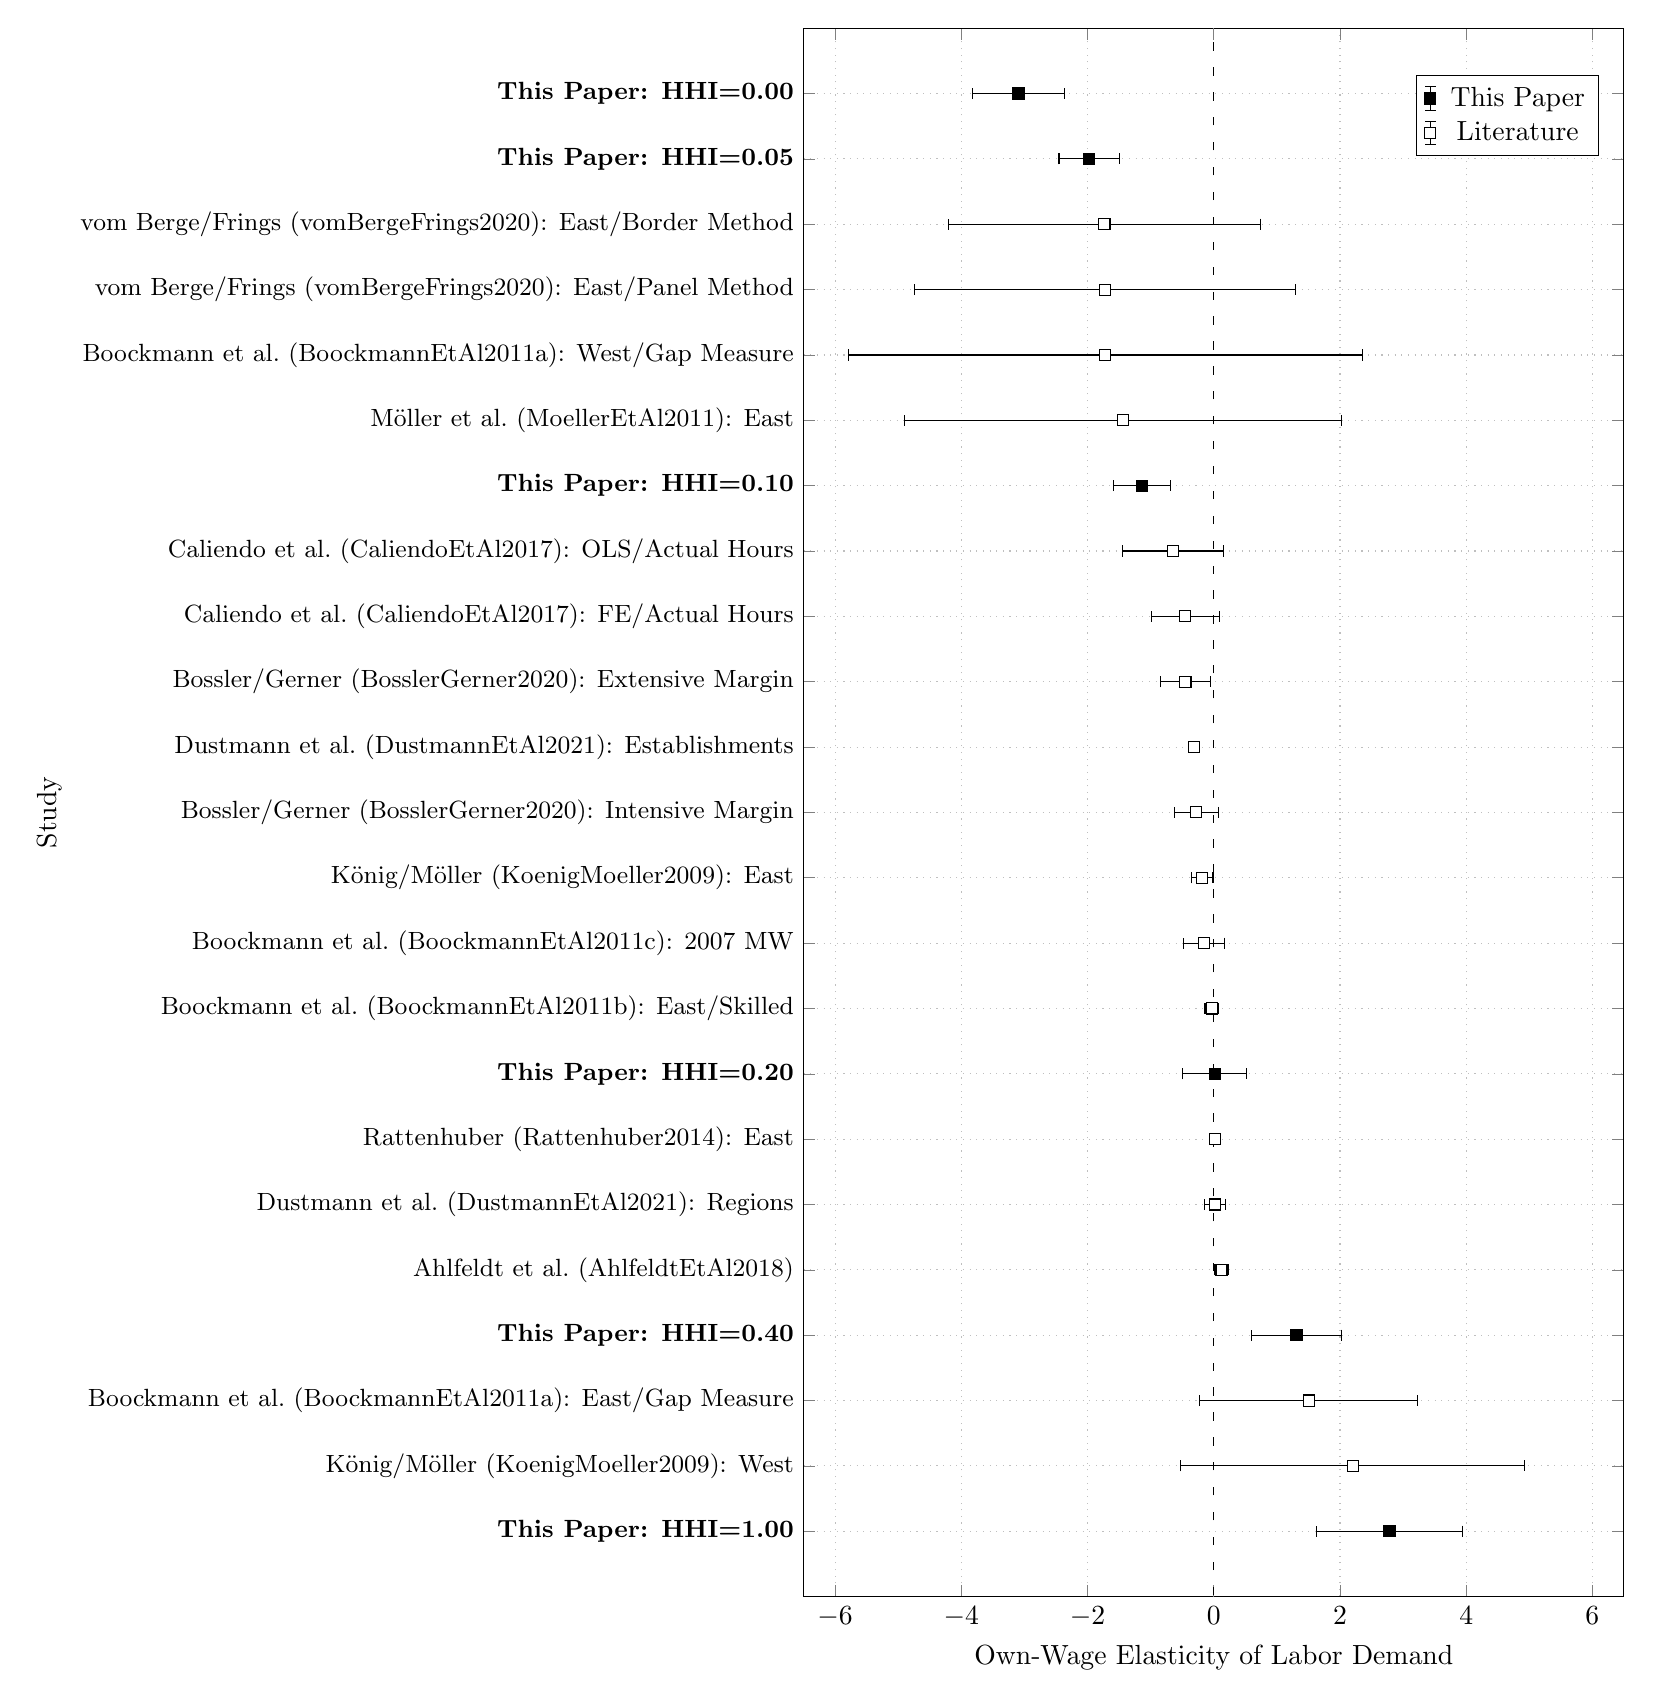
\begin{tikzpicture}
\begin{axis}[ xlabel=Own-Wage Elasticity of Labor Demand, ylabel=Study, height=21.5cm, width=12cm, grid=major, grid style=dotted, xmin=-6.5, xmax=6.5, ymin=0, ymax=24, xtick={-6,-4,-2,2,4,6}, extra x tick style={grid=none}, extra x ticks={0}, legend pos= north east, x tick label style={/pgf/number format/.cd,fixed,fixed zerofill, precision=0,/tikz/.cd},y tick label style = {font=\small}, ytick={1,2,3,4,5,6,7,8,9,10,11,12,13,14,15,16,17,18,19,20,21,22,23}, yticklabels={{\textbf{This Paper: HHI=1.00}\vphantom{/}},{König/Möller (\citeyear{KoenigMoeller2009}): West\vphantom{/}},{Boockmann et al.\ (\citeyear{BoockmannEtAl2011a}): East/Gap Measure\vphantom{/}},{\textbf{This Paper: HHI=0.40}\vphantom{/}},{Ahlfeldt et al.\ (\citeyear{AhlfeldtEtAl2018})\vphantom{/}},{Dustmann et al.\ (\citeyear{DustmannEtAl2021}): Regions\vphantom{/}},{Rattenhuber (\citeyear{Rattenhuber2014}): East\vphantom{/}},{\textbf{This Paper: HHI=0.20}\vphantom{/}},{Boockmann et al.\ (\citeyear{BoockmannEtAl2011b}): East/Skilled\vphantom{/}},{Boockmann et al.\ (\citeyear{BoockmannEtAl2011c}): 2007 MW\vphantom{/}},{König/Möller (\citeyear{KoenigMoeller2009}): East\vphantom{/}},{Bossler/Gerner (\citeyear{BosslerGerner2020}): Intensive Margin\vphantom{/}},{Dustmann et al.\ (\citeyear{DustmannEtAl2021}): Establishments\vphantom{/}},{Bossler/Gerner (\citeyear{BosslerGerner2020}): Extensive Margin\vphantom{/}},{Caliendo et al.\ (\citeyear{CaliendoEtAl2017}): FE/Actual Hours\vphantom{/}},{Caliendo et al.\ (\citeyear{CaliendoEtAl2017}): OLS/Actual Hours\vphantom{/}},{\textbf{This Paper: HHI=0.10}\vphantom{/}},{Möller et al.\ (\citeyear{MoellerEtAl2011}): East\vphantom{/}},{Boockmann et al.\ (\citeyear{BoockmannEtAl2011a}): West/Gap Measure\vphantom{/}},{vom Berge/Frings (\citeyear{vomBergeFrings2020}): East/Panel Method\vphantom{/}},{vom Berge/Frings (\citeyear{vomBergeFrings2020}): East/Border Method\vphantom{/}},{\textbf{This Paper: HHI=0.05}\vphantom{/}},{\textbf{This Paper: HHI=0.00}\vphantom{/}},}]
\addplot[only marks,mark=square*,color=black, error bar legend, error bars/.cd, x dir=both, x explicit] coordinates {  (2.785459,1)+-(1.1535403,0) (1.3124577,4)+-(.70962298,0) (.01452557,8)+-(.50645363,0) (-1.1377976,17)+-(.44608831,0) (-1.9705763,22)+-(.48202872,0) (-3.0937417,23)+-(.73409605,0) };
\addplot[only marks,mark=square*, mark options={fill=white}, color=black, error bar legend, error bars/.cd, x dir=both, x explicit] coordinates {  (2.2,2)+-(2.7201755,0) (1.5037168,3)+-(1.7227291,0) (.12244898,5)+-(.10369049,0) (.02569343,6)+-(.16569343,0) (.02469136,7)+-(.08243902,0) (-.03333334,9)+-(.10504049,0) (-.15625,10)+-(.32598916,0) (-.18181819,11)+-(.17034537,0) (-.278,12)+-(.34873998,0) (-.31,13)+-(.06580001,0) (-.449,14)+-(.39151001,0) (-.44927537,15)+-(.53441226,0) (-.64864862,16)+-(.79794633,0) (-1.4366198,18)+-(3.4612236,0) (-1.7183124,19)+-(4.0736532,0) (-1.7238095,20)+-(3.0174115,0) (-1.7325581,21)+-(2.4758172,0) };
\addplot[loosely dashed] coordinates {(0,-1.5) (0,24.5)};
\legend{~This Paper,~Literature}
\end{axis}
\end{tikzpicture}
}  %\vspace*{-0.5cm}
\floatfoot{ \footnotesize \textsc{Note. ---} The figure gives an overview of own-wage elasticities of labor demand from the minimum wage literature on Germany. Solid squares represent estimated own-wage elasticities of labor demand that originate from this study (at varying levels of labor market concentration) whereas hollow squares depict elasticities from the literature. Each point estimate features a 90 percent confidence interval. For estimates from this study, I calculate own-wage elasticities of labor demand at certain HHI levels by dividing the minimum wage elasticity of employment from Column (4) in Table \ref{tab:3} by the minimum wage elasticity of earnings from Column (4) in Table \ref{tab:2}. The respective standard errors stem from a Bootstrap algorithm with 50 replications. For studies from the literature that do not explicitly report the own-wage elasticity of labor demand, I calculate the ratio of minimum wage elasticities of employment to the respective minimum wage elasticities of earnings by myself. Moreover, if the standard error of the wage elasticity of labor demand is not documented, I apply the Delta method to reported coefficients and their standard errors and assume that the covariance between wage and employment effects is zero. The figure does not include elasticities for which the minimum wage did not bite (i.e., studies without significantly positive minimum wage effects on earnings). To ensure comparability with this paper's empirical approach, I also do not take into account (semi-)structural estimations as well as simulations of minimum wages.  FE = Fixed Effects Estimator. HHI = Herfindahl-Hirschman Index. MW = Minimum Wage. OLS = Ordinary Least Squares. Sources: IEB $\plus$ BHP $\plus$ IAB Establishment Panel, 1999-2017.}
\end{figure}
}



\section{Conclusion}
\label{sec:9}

%summary: contribution
For many years, minimum wages have sparked contentious debates in both scientific and political spheres. While opponents warn that higher minimum wages hurt jobs, proponents argue that such a policy would not only raise wages but, in monopsonistic labor markets, also stimulate employment. In the last two decades, a growing volume of work has reported close-to-zero employment effects, thus lending some support to the monopsony theory. Unfortunately, direct empirical evidence that systematically attributes small or positive employment effects to the presence of monopsony power is rare, and as yet not available for Germany. In this paper, I follow the classical notion of thin labor markets and use detailed measures of labor market concentration to quantify the degree of monopsonistic competition in Germany. Building on these proxies, I inspect whether labor market concentration modulates the impact of higher sectoral minimum wages on employment.

%summary: results

I take advantage of administrative data on the universe of workers liable to social security contribution and provide first evidence on labor market concentration in Germany, an important but hitherto unavailable friction parameter. The concentration measures challenge the traditional view that labor markets exhibit an atomistic market structure. Rather, labor market concentration turns out to be substantial: across alternative labor market definitions, different indicators and regardless whether the accumulation of employment or new hires is looked upon. While the degree varies widely between labor markets, I document that average concentration has remained relatively stable since the turn of the millennium.

The empirical analysis aims to inject more empirical substance into the minimum wage debate. Before analyzing minimum wages, however, I explore whether a policy intervention is required at all to correct for market failure. In fact, the results show that firms successfully lower both earnings and employment in concentrated labor markets, which is suggestive of monopsonistic wage-setting power. Specifically, a 10 percent increase in HHI implies a reduction in earnings by 0.5 percent and a decline in employment by 1.6 percent.

In a first step of the minimum wage analysis, I show that sectoral minimum wage are binding -- both in West and East Germany. The bite becomes larger in more concentrated labor markets, thus corroborating the proposition from monopsony theory and the present evidence that firms in highly concentrated markets exploit their workers. In line with perfect competition, higher sectoral minimum wages harm employment in slightly concentrated markets. Crucially, however, the disemployment effect gradually disappears for increasing labor market concentration such that highly concentrated markets feature job growth, as put forward by the monopsony argument. However, when the level of the sectoral minimum wage draws nearer to firms' median wages, the positive employment effects in highly concentrated labor markets quickly disappear. All in all, the regression results corroborate the theoretical paradigms of both perfect competition and monopsony. But, neither model alone suffices to reflect the observed effect heterogeneity. Instead, the estimated pattern of elasticities advocates a more nuanced view, namely that the minimum wage effects on earnings and employment systematically differ depending on the underlying market structure.


%policy implications
This study bears important policy implications. Antitrust policy in Germany and the E.U.\ focuses on consumer welfare by preventing distortions in product markets. However, the analysis demonstrates that many firms also enjoy considerable power in labor markets, with detrimental effects to earnings and employment. Hence, antitrust authorities should scrutinize mergers, collusive practices, and other non-competitive behavior also in view of a potential supremacy of employers over workers. For this purpose, \citet{NaiduEtAl2018} develop antitrust remedies for labor market power. Alternatively, the existence of powerful worker unions may counteract monopsony power. If both antitrust policy or worker unions fail to correct for monopsony power in the first place, an adequately set minimum wage constitutes a welfare-enhancing policy when monopsony power is widespread \citep{BergerEtAl2019}, reinforcing both wages and employment at the lower end of the earnings distribution. In the German case, the constructed concentration measures can provide standardized guidance to policymakers whether or not certain labor markets would benefit from a minimum wage legislation. However, when the minimum wage is set universally, the benefits of counteracting monopsonistic exploitation in concentrated labor markets might be outweighed by job losses in slightly concentrated labor markets. Moreover, an excessively high minimum wage may deteriorate employment even in highly concentrated labor markets.


%future research
Prior work has largely ignored that the minimum wage effect on employment varies systematically by market structure, thus reporting hybrid elasticities that are close to zero. Future research should acknowledge the underlying heterogeneity and increasingly test for the role of monopsony power or a proxy thereof. Additional work that examines the empirical connection between the labor supply elasticity to the firm and labor market concentration, the classical source of monopsony power, would prove insightful. Apart from labor market concentration, future work should envisage further parameters that capture ``modern'' sources of monopsony power like search cost or idiosyncratic preferences -- factors that may additionally moderate minimum wage effects.







\clearpage

\printbibliography[heading=bibintoc] % bibliography
%\addcontentsline{toc}{section}{\protect\numberline{}References}


\clearpage












% appendix

\clearpage
\begin{appendix}
\renewcommand\thetable{\thesection\arabic{table}} % arabic numbering for tables
\renewcommand\thefigure{\thesection\arabic{figure}} % arabic numbering for figures
\begin{refsection} % define new bibliography for appendix


\begin{landscape}



\section*{Online Appendix}

\section{Appendix: Theoretical Model}
\label{sec:A}
\setcounter{table}{0} % reset table counter
\setcounter{figure}{0} % reset figure counter

\vspace{\fill}

\begin{figure}[!ht]
\centering
\caption{Labor Market Outcomes by Market Structure}
\label{fig:A1}

\huge
\begin{center}

\scalebox{0.7}{
%\begin{tikzpicture}[every node/.style={color=iab_darkcerulean}, dot/.style={circle,fill=iab_darkcerulean,minimum size=8pt,inner sep=0pt,outer sep=-1pt}]

\begin{tikzpicture}[line width=0.8pt, every node/.style={color=black}, dot/.style={circle,fill=black,minimum size=6pt,inner sep=0pt,outer sep=-1pt}]

\draw[<->,thick, xshift=-1.3cm, line width=2pt,rounded corners=0.1cm]  (0,13) node(yline)[above]{$\bm{w}$} -- (0,1) -- (13,1) node(xline)[right]{$\bm{L}$};
%\draw[->,thick, xshift=-1.3cm] (0,0) -- (0,13) node(yline)[above]{$\bm{w}$};
\draw[xshift=-1.3cm] (1.3,11.7) -- (11.7,4.3) node[below]{ \shortstack{ \textbf{LD}  \\ \textbf{MRPL}  } };
\draw[xshift=-1.3cm] (1.3,1.3) -- (11.7,8.7) node[above]{\textbf{LS}};

\draw[xshift=-1.3cm] (1.3,2.2262) -- (7.952949,11.7) node[above]{\textbf{MCL}};

\draw[dash pattern = on 6pt off 3pt,xshift=-1.3cm] (0,6.5) -- (8.602528,6.5) -- (8.602528,1);
\draw[xshift=-1.3cm] (8.602528,1) -- (8.602528,1) node[below]{$L^{C}$};
\draw[xshift=-1.3cm] (0,6.5) -- (0,6.5) node[left]{$w^{C}$};




\draw[dash pattern = on 6pt off 3pt,xshift=-1.3cm]  (5.735018727,4.458333334) -- (0,4.458333334) node[left]{$w^{M}$};
\draw[dash pattern = on 6pt off 3pt,xshift=-1.3cm]  (5.735018727,8.54166667) -- (5.735018727,1) node[below]{$L^{M}$};


\draw[dash pattern = on 6pt off 3pt,xshift=-1.3cm]   (5.735018727,8.54166667) -- (0,8.54166667)  node[left]{$\overline{w}$};



\draw[dotted, xshift=-1.3cm, thick] (11.7,7.52083335) -- (0,7.52083335) node[left]{$w^{min}$};
\draw[dash pattern = on 6pt off 3pt,xshift=-1.3cm] (7.1687773385,7.52083335) -- (7.1687773385,1) node[below]{$L^{min}$};



\node[dot,xshift=-1.3cm] at (7.1687773385,7.52083335) {};
\node[dot,xshift=-1.3cm] at (5.735018727,4.458333334) {};
\node[dot,xshift=-1.3cm] at (5.735018727,8.54166667) {};
\node[dot,xshift=-1.3cm] at (8.602528,6.5) {};

\end{tikzpicture}
}
\end{center}
\normalsize
\floatfoot{ \footnotesize \textsc{Note. ---} The figure compares labor market outcomes between the polar cases of perfect competitive and monopsonistic labor markets. Moreover, the diagram shows the effects from introducing an exemplary minimum wage above but close to the equilibrium wage rate (i.e., in the range of the demand-determined regime). Source: Own illustration.}

\end{figure}

%\vspace*{2.5cm}
\vspace*{\fill}
\end{landscape}

\clearpage
\vspace*{\fill}

\begin{figure}[!ht]
\centering
\caption{Stylized Minimum Wage Effects by Market Structure}
\label{fig:A2}
\vspace*{0.5cm}
\begin{subfigure}{1\textwidth}
\centering
\caption{Minimum Wage Effects on Earnings}
\scalebox{0.85}{
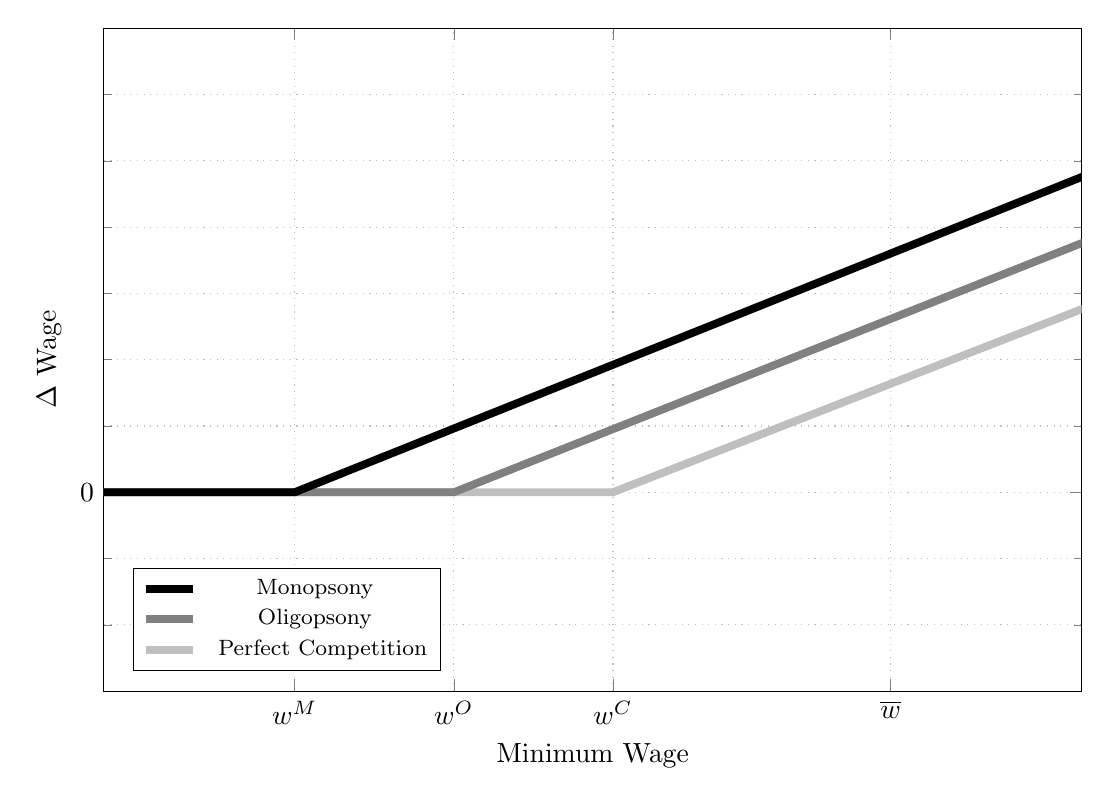
\begin{tikzpicture}

\begin{axis}[height=10cm, width=14cm, grid=both, grid style = dotted,ytick={0},minor ytick={-2,-1,0,1,2,3,4,5,6}, xtick={3,5.5,8,12.363636}, xlabel=Minimum Wage, ylabel=$\Delta$ Wage, ymin=-3, ymax=7, xmin=0, xmax=15.363636, legend pos = south west, y tick label style={/pgf/number format/.cd,fixed,fixed zerofill, precision=0,/tikz/.cd}, x tick label style={/pgf/number format/.cd,fixed,fixed zerofill, precision=1,/tikz/.cd}, legend style={font=\footnotesize}, reverse legend, xticklabels={$w^{M}$,$w^{O}$,$w^{C}$,$\overline{w}$}]



\addplot[mark=none, solid, color=lightgray, line width=1mm] coordinates { (0,0) (8,0) (16,3) };
\addplot[mark=none, solid, color=gray, line width=1mm] coordinates { (0,0) (5.5,0) (16,4) };
\addplot[mark=none, solid, color=black, line width=1mm] coordinates { (0,0) (3,0) (16,5) };


\legend{~~Perfect Competition, Oligopsony, Monopsony}
\end{axis}
\end{tikzpicture}
}
\end{subfigure}
\vskip \baselineskip \vspace*{0.5cm}
\begin{subfigure}{1\textwidth}
\centering
\caption{Minimum Wage Effects on Employment}
\scalebox{0.85}{
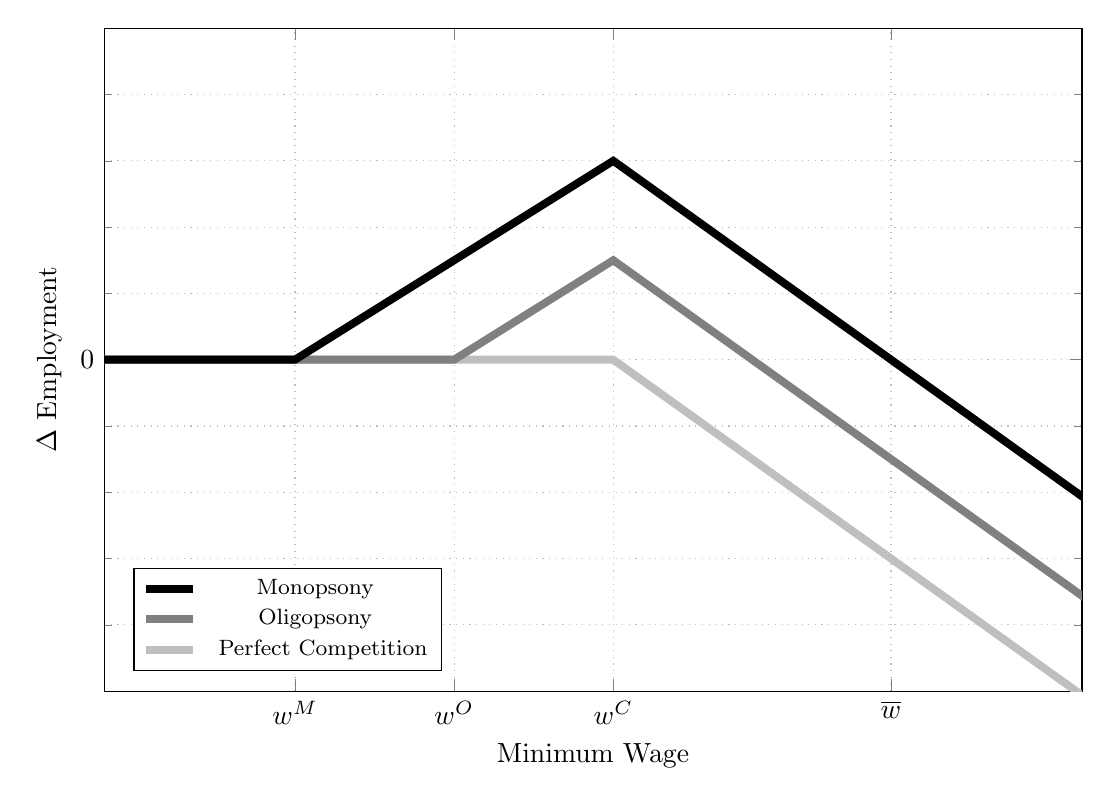
\begin{tikzpicture}

\begin{axis}[height=10cm, width=14cm, grid=both, grid style = dotted,ytick={0},minor ytick={-4,-3,-2,-1,0,1,2,3,4}, xtick={3,5.5,8,12.363636}, xlabel=Minimum Wage, ylabel=$\Delta$ Employment, ymin=-5, ymax=5, xmin=0, xmax=15.363636, legend pos = south west, y tick label style={/pgf/number format/.cd,fixed,fixed zerofill, precision=0,/tikz/.cd}, x tick label style={/pgf/number format/.cd,fixed,fixed zerofill, precision=1,/tikz/.cd}, legend style={font=\footnotesize}, reverse legend, xticklabels={$w^{M}$,$w^{O}$,$w^{C}$,$\overline{w}$}]



\addplot[mark=none, solid, color=lightgray, line width=1mm] coordinates { (0,0) (8,0) (16,-5.5) };
\addplot[mark=none, solid, color=gray, line width=1mm] coordinates { (0,0) (5.5,0) (8,1.5) (16,-4)  };
\addplot[mark=none, solid, color=black, line width=1mm] coordinates { (0,0) (3,0) (8,3) (16,-2.5)};

\legend{~~Perfect Competition, Oligopsony, Monopsony}
\end{axis}
\end{tikzpicture}
}
\end{subfigure}

\floatfoot{ \footnotesize \textsc{Note. ---} The figures visualize minimum wage effects on wages and employment within the general framework of a Cournot oligopsony of identical firms (i.e., in the symmetric case). The x axis refers to absolute levels of minimum wages whereas the y axis shows absolute deviations from the free-market level of the outcome variable. The linearity of employment effects derives from the assumption that both marginal product of labor and labor supply to the firm/market are first-order polynomials in the wage rate. Due to the symmetry assumption, market- and firm-level employment effects feature identical signs. Source: Own illustration.}
\end{figure}


\vspace*{\fill}
\clearpage


\begin{landscape}


\section{Appendix: Institutional Framework}
\label{sec:B}
\setcounter{table}{0} % reset table counter
\setcounter{figure}{0} % reset figure counter

\vspace*{-0.25cm}

\begin{table}[!ht]
\centering

\renewcommand{\arraystretch}{1.4}
\scalebox{0.85}{

\begin{threeparttable}
\caption{Minimum Wage Legislation in Germany}
\label{tab:B1}
\vspace{-0.1cm}
\begin{tabular}[c]{|C{5.5cm}|C{8cm}:C{5.25cm}:C{8.75cm}|} \hline \hline



\multirow{3}{*}{\diagbox[height=4.2\line, innerwidth=5.5cm]{Law}{Dimension}}  & \multirow{3}{*}{\shortstack{Prerequisites for \vphantom{/} \\ Declaration of Universal Bindingness \vphantom{/} }} & \multirow{3}{*}{upon Approval by ...\vphantom{/}} & \multirow{3}{*}{Possible Scope\vphantom{/}} \\
&&& \\
%&&& \\
&&& \\ \hline		

\multirow{4}{*}{\shortstack{\textbf{TVG (1949, 1969, 2014)}\vphantom{/}\\[0.1cm] valid: 04/1949-hitherto \vphantom{/}}}  &  \multirow{4}{*}{\shortstack{\tabitem MW regulation in existing CBA\vphantom{/} \\ \tabitem request from a CBA partner\vphantom{/}\\ \tabitem firms s.t.\ CBA $>$ 50\% (until 08/2014) \vphantom{/}\\ \tabitem in public interest \vphantom{/} }} &  \multirow{4}{*}{\shortstack{\tabitem Bargaining Committee\vphantom{/}\\ \tabitem BMAS \vphantom{/}}} & \multirow{4}{*}{\tabitem sectoral\vphantom{/}}  \\
&&& \\
&&& \\
&&& \\ \hdashline


\multirow{2}{*}{\shortstack{\textbf{AEntG (1998, 2007)}\vphantom{/}\\[0.1cm] valid: 01/1999-04/2009 \vphantom{/}}}    &  \multirow{2}{*}{\shortstack{\tabitem MW regulation in existing CBA\vphantom{/} \\ \tabitem request from a CBA partner\vphantom{/}}} &  \multirow{2}{*}{\tabitem BMAS\vphantom{/}} & \multirow{2}{*}{\shortstack{\tabitem sector-wise in construction industry\vphantom{/}\\ \tabitem commercial cleaning (since 07/2007)\vphantom{/} }}   \\
&&& \\ \hdashline



\multirow{3}{*}{\shortstack{\textbf{AEntG (2009, 2014)}\vphantom{/}\\[0.1cm] valid: 04/2009-hitherto \vphantom{/}}}   &  \multirow{3}{*}{\shortstack{\tabitem MW regulation in existing CBA\vphantom{/} \\ \tabitem joint request from CBA partners\vphantom{/} \\ \tabitem in public interest\vphantom{/}}} &  \multirow{3}{*}{\shortstack{\tabitem BMAS\vphantom{/} \\  (\tabitem Bargaining Committee) \vphantom{/} \\ (\tabitem Federal Government) \vphantom{/}}} & \multirow{3}{*}{\shortstack{\tabitem sector-wise in nine industries (until 08/2014)\vphantom{/}\\ \tabitem sector-wise (since 08/2014)\vphantom{/}}}   \\
&&& \\
&&& \\ \hdashline



\multirow{4}{*}{\shortstack{\textbf{AÜG (2011, 2014)}\vphantom{/}\\ valid: 12/2011-hitherto \vphantom{/}}}  &  \multirow{4}{*}{\shortstack{\tabitem MW regulation in existing CBA\vphantom{/} \\ \tabitem joint request from CBA partners\vphantom{/} \\ \tabitem MW beneficial for social security system\vphantom{/} \\ \tabitem in public interest (since 08/2014)\vphantom{/}}} &  \multirow{4}{*}{\tabitem BMAS\vphantom{/}} & \multirow{4}{*}{\tabitem temporary work\vphantom{/}}   \\
&&& \\
&&& \\
&&& \\ \hdashline



\multirow{2}{*}{\shortstack{\textbf{MiLoG (2014)}\vphantom{/}\\[0.1cm] valid: 01/2015-hitherto \vphantom{/}}}  &  \multirow{2}{*}{none} &  \multirow{2}{*}{\tabitem MW Commission\vphantom{/}} & \multirow{2}{*}{\tabitem nation-wide\vphantom{/}}   \\

&&& \\ \hline \hline

\end{tabular}

\begin{tablenotes}
\item  \footnotesize \textsc{Note. ---} The table describes the pieces of legislation that regulate the imposition of minimum wages in in Germany. With respect to TVG (1949, 1969, 2014) and AEntG (2009, 2014), the Bargaining Committee consists of six members, three of whom are appointed from each of the national umbrella organizations of employees and employers. For the AEntG (2009, 2014), initial declaration requests for a specific collective bargaining agreement in a certain sector need approval of both the BMAS and the Bargaining Committee (at least four yes-votes from six members or, alternatively, tacit approval after three months) or the Federal Government (if there are only two or three yes-votes in the Bargaining Committee). On the contrary, follow-up requests for subsequent collective agreements in the same sector merely require approval of the BMAS. The nine industries listed in AEntG (2009) as candidates for sectoral minimum are: construction, commercial cleaning, postal services, security, specialized hard coal mining, industrial laundries, waste removal, public training services from SGB II/III, and nursing care. According to MiLoG (2014), the Minimum Wage Commission consists of a chairperson, three employee and three employer representatives and two non-voting advisory members from the scientific community. AEntG = Arbeitnehmerentsendegesetz. AÜG = Arbeitnehmerüberlassungsgesetz. BMAS = Federal Ministry for Labor and Social Affairs. CBA = Collective Bargaining Agreement. MiLoG = Mindestlohngesetz. MW = Minimum Wage. SGB II/III = Sozialgesetzbuch II/III. s.t. = subject to. TVG = Tarifvertragsgesetz. Sources: AEntG $\plus$ AÜG $\plus$ MiLoG $\plus$ TVG.
\end{tablenotes}


\end{threeparttable}
}
\end{table}



\clearpage



\begin{table}[!ht]

\centering

\renewcommand{\arraystretch}{1.5}
\scalebox{0.85}{

\begin{threeparttable}
\caption{Sectoral Minimum Wages}
\label{tab:B2}
\vspace{-0.1cm}
\begin{tabular}[c]{|C{6.5cm}|C{2.25cm}C{4cm}:C{2.5cm}C{2cm}C{3cm}:C{6cm}|} \hline \hline



\multirow{2}{*}{\diagbox[height=3\line, innerwidth=6.5cm]{Sector}{Dimension}} & \multirow{2.4}{*}{\shortstack{First\vphantom{/} \\ MW\vphantom{/}}}   & \multirow{2.4}{*}{Legislative Basis\vphantom{/} }  & \multirow{2.4}{*}{\shortstack{Establish-\vphantom{/} \\ ments\vphantom{/}}} & \multirow{2.4}{*}{Workers} & \multirow{2.4}{*}{\shortstack{Kaitz Index\vphantom{/} \\ (West/East)\vphantom{/} }} & \multirow{2.4}{*}{2008 NACE-5 Classification:\vphantom{/}} \\


&&&&&& \\ \hline		

\multirow{2}{*}{Main Construction} &  \multirow{2}{*}{01/1997}   &  \multirow{2}{*}{TVG/AEntG}  & \multirow{2}{*}{82,166} & \multirow{2}{*}{793,738} &  \multirow{2}{*}{0.66/0.86} & \multirow{1}{*}{4120.1-4299.0/4312.0/4329.1} \\[-0.2cm]

&&&&&& \multirow{1}{*}{4331.0/4391.2/4399.2/4399.9} \\ \hdashline

\multirow{1}{*}{Electrical Trade} &  \multirow{1}{*}{06/1997}   &  \multirow{1}{*}{TVG/MiLoG}  & \multirow{1}{*}{29,760} & \multirow{1}{*}{246,196} &  \multirow{1}{*}{0.66/0.84} & \multirow{1}{*}{4321.0} \\ \hdashline

\multirow{1}{*}{Roofing} &  \multirow{1}{*}{10/1997}   &  \multirow{1}{*}{TVG/AEntG}  & \multirow{1}{*}{12,995} & \multirow{1}{*}{89,830} &  \multirow{1}{*}{0.74/0.99} &  \multirow{1}{*}{4391.1} \\ \hdashline

\multirow{1}{*}{Painting \& Varnishing} &  \multirow{1}{*}{12/2003}   &  \multirow{1}{*}{AEntG}  & \multirow{1}{*}{23,706} & \multirow{1}{*}{141,125} &  \multirow{1}{*}{0.67/0.91} & \multirow{1}{*}{4334.1} \\ \hdashline


\multirow{1}{*}{Commercial Cleaning} &  \multirow{1}{*}{04/2004}   &  \multirow{1}{*}{TVG/AEntG/MiLoG}  & \multirow{1}{*}{29,628} & \multirow{1}{*}{919,563} &  \multirow{1}{*}{0.83/0.95} & \multirow{1}{*}{8121.0/8122.9-8129.9} \\ \hdashline



\multirow{1}{*}{Waste Removal} &  \multirow{1}{*}{01/2010}   &  \multirow{1}{*}{AEntG/MiLoG}  & \multirow{1}{*}{6,872} & \multirow{1}{*}{177,647} &  \multirow{1}{*}{0.52/0.73} & \multirow{1}{*}{3811.0-3900.0} \\ \hdashline

\multirow{1}{*}{Nursing Care} &  \multirow{1}{*}{08/2010}   &  \multirow{1}{*}{AEntG}  & \multirow{1}{*}{21,372} & \multirow{1}{*}{939,660} &  \multirow{1}{*}{0.60/0.71} & \multirow{1}{*}{8710.0/8810.1}  \\ \hdashline

\multirow{1}{*}{Security} &  \multirow{1}{*}{06/2011}   &  \multirow{1}{*}{AEntG/MiLoG}  & \multirow{1}{*}{4,735} & \multirow{1}{*}{196,032} &  \multirow{1}{*}{0.80/0.87} & \multirow{1}{*}{8010.0/8020.0} \\ \hdashline


\multirow{1}{*}{Temporary Work} &  \multirow{1}{*}{01/2012}   &  \multirow{1}{*}{AÜG/MiLoG}  & \multirow{1}{*}{12,355} & \multirow{1}{*}{829,579} &  \multirow{1}{*}{0.80/0.87} & \multirow{1}{*}{7820.0/7830.0}   \\ \hdashline


\multirow{1}{*}{Scaffolding} &  \multirow{1}{*}{08/2013}   &  \multirow{1}{*}{AEntG/MiLoG} & \multirow{1}{*}{2,862} & \multirow{1}{*}{28,935}  &  \multirow{1}{*}{0.69/0.87} & \multirow{1}{*}{4399.1} \\ \hdashline

\multirow{1}{*}{Stonemasonry} &  \multirow{1}{*}{10/2013}   &  \multirow{1}{*}{AEntG/MiLoG}  & \multirow{1}{*}{4,314} & \multirow{1}{*}{25,443} &  \multirow{1}{*}{0.73/0.93} & \multirow{1}{*}{2370.0}   \\ \hdashline

\multirow{1}{*}{Hairdressing} &  \multirow{1}{*}{11/2013}   &  \multirow{1}{*}{TVG/AEntG/MiLoG}  & \multirow{1}{*}{48,976} & \multirow{1}{*}{193,559} &  \multirow{1}{*}{1.02/1.11} & \multirow{1}{*}{9602.1}   \\ \hdashline

\multirow{1}{*}{Chimney Sweeping} &  \multirow{1}{*}{04/2014}   &  \multirow{1}{*}{TVG}  & \multirow{1}{*}{7,428} & \multirow{1}{*}{16,728} &  \multirow{1}{*}{0.73/0.88} & \multirow{1}{*}{8122.1}   \\ \hdashline

\multirow{1}{*}{Slaughtering \& Meat Processing} &  \multirow{1}{*}{08/2014}   &  \multirow{1}{*}{AEntG}  & \multirow{1}{*}{9,549} & \multirow{1}{*}{182,504} &  \multirow{1}{*}{0.66/0.88} & \multirow{1}{*}{1011.0-1013.0}   \\ \hdashline

\multirow{1}{*}{Textile \& Clothing} &  \multirow{1}{*}{01/2015}   &  \multirow{1}{*}{AEntG/MiLoG}  & \multirow{1}{*}{6,398} & \multirow{1}{*}{120,099} &  \multirow{1}{*}{0.54/0.76} & \multirow{1}{*}{1310.0-1439.0}   \\ \hdashline

\multirow{1}{*}{Agriculture, Forestry \& Gardening} &  \multirow{1}{*}{01/2015}   &  \multirow{1}{*}{AEntG}  & \multirow{1}{*}{79,056} & \multirow{1}{*}{342,451} &  \multirow{1}{*}{0.70/0.73} & \multirow{1}{*}{111.0-240.0/312.0-322.0}   \\ \hline \hline


\end{tabular}

\begin{tablenotes}
\item  \footnotesize \textsc{Note. ---} The table provides an overview about sectoral minimum wages in Germany. The sectors are arranged in chronological order of their first minimum wage implementation. The overall number of establishments and workers per sector refers to June 30, 2015. I report the Kaitz Index, the sectoral minimum wage on 1 Jan 2015 divided by the median wage of regular full-time workers per sector on 30 June 2014, separately for West (left) and East Germany (right) excluding Berlin. The 5-digit industry codes from the 2008 version of the German NACE Classification serve to identify the sectoral affiliation of establishments between 2008 and 2017. For the years 1999-2002 and 2003-2007, I make use of earlier 1993 NACE-5 and 2003 NACE-5 codes to determine the minimum wage sectors. For reasons of parsimony, this table does not review the following minimum wage sectors that cannot be identified by means of available industry codes: industrial laundries, specialized hard coal mining, public training services as well as money and value services. AEntG = Arbeitnehmerentsendegesetz. AÜG = Arbeitnehmerüberlassungsgesetz.  MiLoG = Mindestlohngesetz. MW = Minimum Wage. NACE-5 = 5-Digit Statistical Nomenclature of Economic Activities in the European Community. TVG = Tarifvertragsgesetz. Sources: AEntG $\plus$ AÜG  $\plus$ IEB, 1999-2017 $\plus$ Bundesanzeiger $\plus$ MiLoG $\plus$ TVG.
\end{tablenotes}


\end{threeparttable}
}
\end{table}



\clearpage




\begin{figure}[!ht]
\centering
\caption{Variation in Sectoral Minimum Wages}
\label{fig:B1}
\begin{subfigure}{0.475\textwidth}
\centering
\caption{Main Construction}
\scalebox{0.825}{
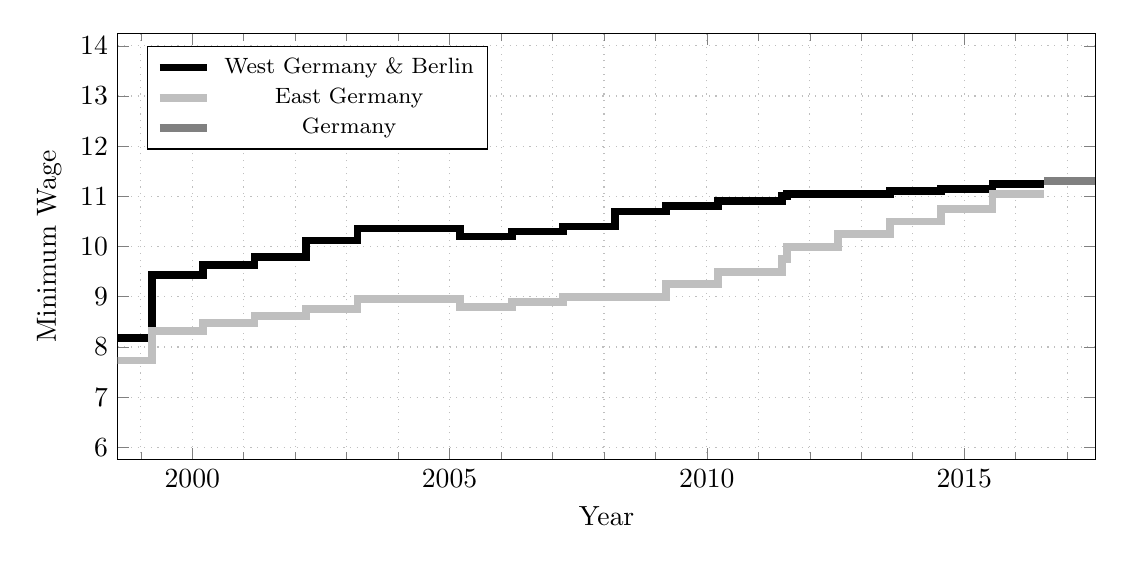
\begin{tikzpicture}

\begin{axis}[ytick={6,7,8,9,10,11,12,13,14}, height=7cm, width=14cm, grid=both, grid style = dotted, xtick={2000.45,2005.45,2010.45,2015.45},minor xtick={1999.45,2001.45,2002.45,2003.45,2004.45,2006.45,2007.45,2008.45,2009.45,2011.45,2012.45,2013.45,2014.45,2016.45,2017.45}, xlabel=Year, ylabel=Minimum Wage, ymin=5.75, ymax=14.25, xmin=1999.00, xmax=2018.00, legend pos = north west, y tick label style={/pgf/number format/.cd,fixed,fixed zerofill, precision=0,/tikz/.cd}, x tick label style={/pgf/number format/.cd,fixed,fixed zerofill, precision=0,/tikz/.cd}, legend style={font=\footnotesize}]

% West Germany and Berlin
\addplot[mark=none, solid, color=black, line width=1mm] coordinates { (1997.00,8.68) (1997.66,8.68) (1997.66,8.17) (1999.66,8.17) (1999.66,9.44) (2000.66,9.44) (2000.66,9.63) (2001.66,9.63) (2001.66,9.79) (2002.66,9.79) (2002.66,10.12) (2003.66,10.12) (2003.66,10.36)  (2003.83,10.36) (2003.83,10.36) (2004.66,10.36) (2004.66,10.36) (2005.66,10.36) (2005.66,10.20) (2006.66,10.20)  (2006.66,10.30) (2007.66,10.30) (2007.66,10.40) (2008.66,10.40) (2008.66,10.70) (2009.66,10.70) (2009.66,10.80) (2010.66,10.80) (2010.66,10.90) (2011.91,10.90) (2011.91,11.00) (2012.00,11.00) (2012.00,11.05) (2013.00,11.05) (2013.00,11.05) (2014.00,11.05) (2014.00,11.10) (2015.00,11.10) (2015.00,11.15) (2016.00,11.15) (2016.00,11.25) (2017.00,11.25) };

% East Germany
\addplot[mark=none, solid, color=lightgray, line width=1mm] coordinates { (1997.00,7.98) (1997.66,7.98) (1997.66,7.73) (1999.66,7.73) (1999.66,8.31) (2000.66,8.31) (2000.66,8.47) (2001.66,8.47) (2001.66,8.61) (2002.66,8.61) (2002.66,8.75) (2003.66,8.75) (2003.66,8.95) (2003.83,8.95) (2003.83,8.95) (2004.66,8.95) (2004.66,8.95) (2005.66,8.95) (2005.66,8.80) (2006.66,8.80) (2006.66,8.90) (2007.66,8.90) (2007.66,9.00) (2008.66,9.00) (2008.66,9.00) (2009.66,9.00) (2009.66,9.25) (2010.66,9.25) (2010.66,9.50) (2011.91,9.50) (2011.91,9.75) (2012.00,9.75) (2012.00,10.00) (2013.00,10.00) (2013.00,10.25) (2014.00,10.25) (2014.00,10.50) (2015.00,10.50) (2015.00,10.75) (2016.00,10.75)  (2016.00,11.05) (2017.00,11.05) };

% Germany
\addplot[mark=none, solid, color=gray, line width=1mm] coordinates {(2017.00,11.30) (2018.00,11.30)  }; %(2018.16,8.84) (2018.00,8.84) (2018.16,11.75) (2019.16,11.75) (2019.16,12.20) (2020.00,12.20)


\legend{~West Germany \& Berlin,~East Germany,~Germany,}
\end{axis}
\end{tikzpicture}
}
\end{subfigure}
\hfill
\begin{subfigure}{0.475\textwidth}
\centering
\caption{Electrical Trade}
\scalebox{0.825}{
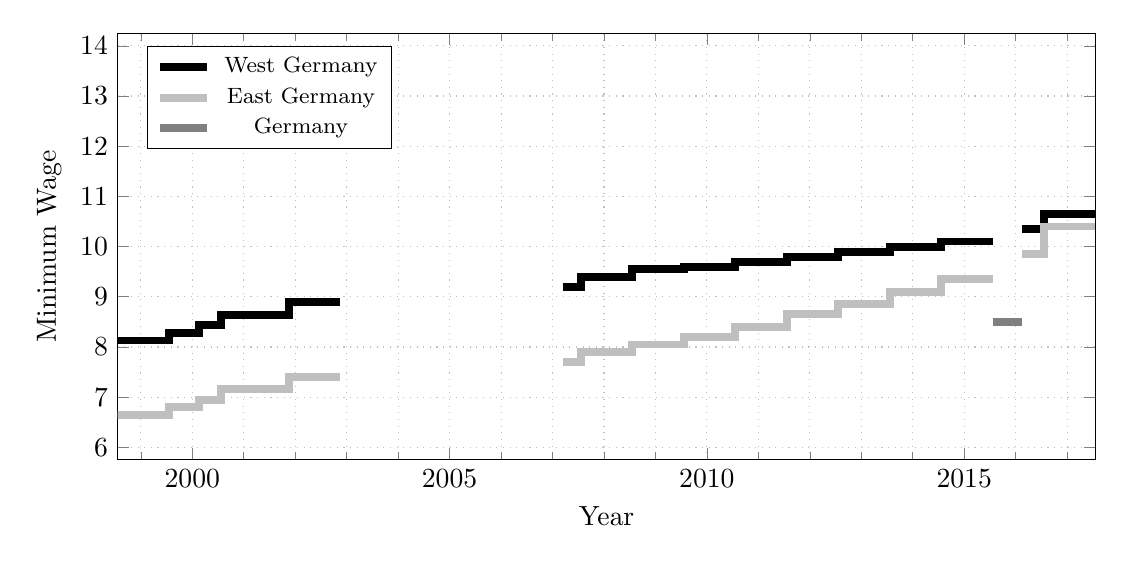
\begin{tikzpicture}

\begin{axis}[ytick={6,7,8,9,10,11,12,13,14}, height=7cm, width=14cm, grid=both, grid style = dotted, xtick={2000.45,2005.45,2010.45,2015.45},minor xtick={1999.45,2001.45,2002.45,2003.45,2004.45,2006.45,2007.45,2008.45,2009.45,2011.45,2012.45,2013.45,2014.45,2016.45,2017.45}, xlabel=Year, ylabel=Minimum Wage, ymin=5.75, ymax=14.25, xmin=1999.00, xmax=2018.00, legend pos = north west, y tick label style={/pgf/number format/.cd,fixed,fixed zerofill, precision=0,/tikz/.cd}, x tick label style={/pgf/number format/.cd,fixed,fixed zerofill, precision=0,/tikz/.cd}, legend style={font=\footnotesize}]

% West Germany and Berlin
\addplot[mark=none, solid, color=black, line width=1mm] coordinates { (1997.41,8.03) (1998.33,8.03) (1998.33,8.13) (1999.66,8.13) (1999.66,8.13) (2000.00,8.13) (2000.00,8.28) (2000.58,8.28)(2000.58,8.44) (2001.00,8.44) (2001.00,8.64) (2001.66,8.64) (2001.66,8.64) (2002.33,8.64) (2002.33,8.90) (2003.33,8.90)};

\addplot[mark=none, solid, color=black, line width=1mm] coordinates { (2007.66,9.20) (2008.00,9.20) (2008.00,9.40) (2009.00,9.40) (2009.00,9.55)  (2010.00,9.55) (2010.00,9.60) (2011.00,9.60) (2011.00,9.70) (2012.00,9.70) (2012.00,9.80) (2013.00,9.80) (2013.00,9.90) (2014.00,9.90) (2014.00,10.00) (2015.00,10.00) (2015.00,10.10) (2016.00,10.10)  };

\addplot[mark=none, solid, color=black, line width=1mm] coordinates { (2016.58,10.35) (2017.00,10.35) (2017.00,10.65) (2018.00,10.65) };


% East Germany
\addplot[mark=none, solid, color=lightgray, line width=1mm] coordinates { (1997.41,6.41) (1998.33,6.41) (1998.33,6.65) (1999.66,6.65) (1999.66,6.65) (2000.00,6.65) (2000.00,6.80) (2000.58,6.80) (2000.58,6.95) (2001.00,6.95) (2001.00,7.16) (2001.66,7.16) (2001.66,7.16) (2002.33,7.16) (2002.33,7.40) (2003.33,7.40) };

\addplot[mark=none, solid, color=lightgray, line width=1mm] coordinates { (2007.66,7.70) (2008.00,7.70) (2008.00,7.90) (2009.00,7.90) (2009.00,8.05)  (2010.00,8.05) (2010.00,8.20) (2011.00,8.20) (2011.00,8.40) (2012.00,8.40) (2012.00,8.65) (2013.00,8.65) (2013.00,8.85) (2014.00,8.85) (2014.00,9.10) (2015.00,9.10) (2015.00,9.35) (2016.00,9.35)    };

\addplot[mark=none, solid, color=lightgray, line width=1mm] coordinates { (2016.58,9.85) (2017.00,9.85) (2017.00,10.40) (2018.00,10.40) };

% Germany
\addplot[mark=none, solid, color=gray, line width=1mm] coordinates { (2016.00,8.50) (2016.58,8.50)   };
%\addplot[mark=none, solid, color=gray, line width=1mm] coordinates {(2018.00,10.95) (2019.00,10.95) (2019.00,11.40) (2020.00,11.40)     };

\legend{~West Germany,,,~East Germany,,,~Germany}
\end{axis}
\end{tikzpicture}
}
\end{subfigure}
\vskip \baselineskip
\begin{subfigure}{0.475\textwidth}
\centering
\caption{Roofing}
\scalebox{0.825}{
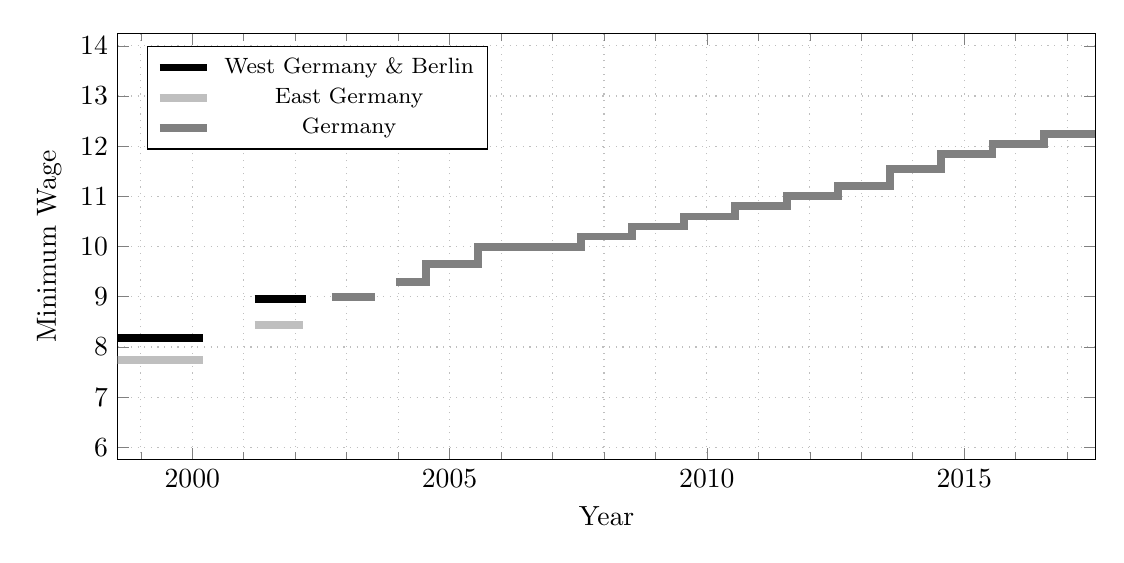
\begin{tikzpicture}

\begin{axis}[ytick={6,7,8,9,10,11,12,13,14}, height=7cm, width=14cm, grid=both, grid style = dotted, xtick={2000.45,2005.45,2010.45,2015.45},minor xtick={1999.45,2001.45,2002.45,2003.45,2004.45,2006.45,2007.45,2008.45,2009.45,2011.45,2012.45,2013.45,2014.45,2016.45,2017.45}, xlabel=Year, ylabel=Minimum Wage, ymin=5.75, ymax=14.25, xmin=1999.00, xmax=2018.00, legend pos = north west, y tick label style={/pgf/number format/.cd,fixed,fixed zerofill, precision=0,/tikz/.cd}, x tick label style={/pgf/number format/.cd,fixed,fixed zerofill, precision=0,/tikz/.cd}, legend style={font=\footnotesize}]


% West Germany and Berlin
\addplot[mark=none, solid, color=black, line width=1mm] coordinates { (1997.75,8.18) (2000.66,8.18)  };
\addplot[mark=none, solid, color=black, line width=1mm] coordinates { (2001.66,8.95) (2002.66,8.95)  };


% East Germany
\addplot[mark=none, solid, color=lightgray, line width=1mm] coordinates { (1997.75,7.74) (2000.66,7.74)   };
\addplot[mark=none, solid, color=lightgray, line width=1mm] coordinates { (2001.66,8.44) (2002.6,8.44)   };

% Germany
\addplot[mark=none, solid, color=gray, line width=1mm] coordinates { (2003.16,9.00) (2004.00,9.00)  };
\addplot[mark=none, solid, color=gray, line width=1mm] coordinates { (2004.41,9.30) (2004.41,9.30) (2005.00,9.30) (2005.00,9.65) (2006.00,9.65) (2006.00,10.00) (2007.00,10.00) (2007.00,10.00) (2008.00,10.00) (2008.00,10.20) (2009.00,10.20) (2009.00,10.40) (2010.00,10.40) (2010.00,10.60) (2011.00,10.60) (2011.00,10.80) (2012.00,10.80) (2012.00,11.00) (2013.00,11.00) (2013.00,11.20) (2014.00,11.20) (2014.00,11.55) (2015.00,11.55) (2015.00,11.85) (2016.00,11.85) (2016.00,12.05) (2017.00,12.05) (2017.00,12.25) (2018.00,12.25)   }; % (2018.00,8.84) (2018.16,8.84) (2018.16,12.20) (2019.00,12.20) (2020.00,12.20)





\legend{~West Germany \& Berlin,,~East Germany,,~Germany,,}
\end{axis}
\end{tikzpicture}
}
\end{subfigure}
\hfill
\begin{subfigure}{0.475\textwidth}
\centering
\caption{Painting \& Varnishing}
\scalebox{0.825}{
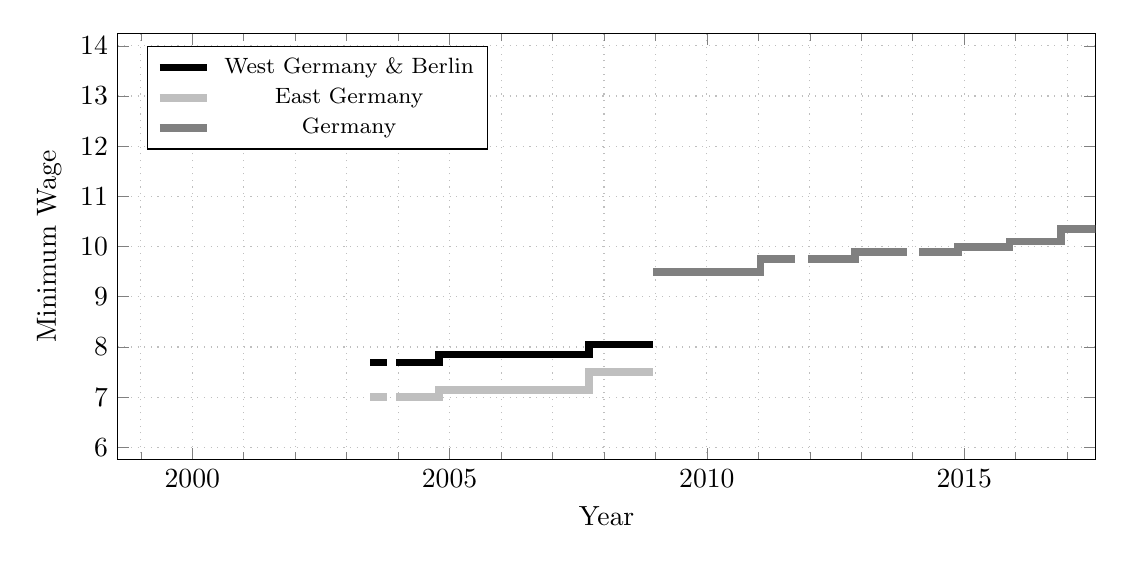
\begin{tikzpicture}

\begin{axis}[ytick={6,7,8,9,10,11,12,13,14}, height=7cm, width=14cm, grid=both, grid style = dotted, xtick={2000.45,2005.45,2010.45,2015.45},minor xtick={1999.45,2001.45,2002.45,2003.45,2004.45,2006.45,2007.45,2008.45,2009.45,2011.45,2012.45,2013.45,2014.45,2016.45,2017.45}, xlabel=Year, ylabel=Minimum Wage, ymin=5.75, ymax=14.25, xmin=1999.00, xmax=2018.00, legend pos = north west, y tick label style={/pgf/number format/.cd,fixed,fixed zerofill, precision=0,/tikz/.cd}, x tick label style={/pgf/number format/.cd,fixed,fixed zerofill, precision=0,/tikz/.cd}, legend style={font=\footnotesize}]

% West Germany and Berlin
\addplot[mark=none, solid, color=black, line width=1mm] coordinates { (2003.91,7.69) (2004.24,7.69)  };
\addplot[mark=none, solid, color=black, line width=1mm] coordinates { (2004.41,7.69) (2005.24,7.69) (2005.24,7.85) (2008.16,7.85)  (2008.16,8.05) (2009.41,8.05)  };


% East Germany
\addplot[mark=none, solid, color=lightgray, line width=1mm] coordinates { (2003.91,7.00) (2004.24,7.00)  };
\addplot[mark=none, solid, color=lightgray, line width=1mm] coordinates { (2004.41,7.00) (2005.24,7.00) (2005.24,7.15) (2008.16,7.15)  (2008.16,7.50) (2009.41,7.50)  };

% Germany
\addplot[mark=none, solid, color=gray, line width=1mm] coordinates { (2009.41,9.50) (2010.66,9.50) (2011.49,9.50) (2011.49,9.75) (2012.16,9.75)  };
\addplot[mark=none, solid, color=gray, line width=1mm] coordinates { (2012.41,9.75)  (2012.49,9.75) (2013.33,9.75) (2013.33,9.90) (2014.33,9.90) };
\addplot[mark=none, solid, color=gray, line width=1mm] coordinates { (2014.58,9.90) (2015.33,9.90) (2015.33,10.00) (2016.33,10.00)  (2016.33,10.10) (2017.33,10.10) (2017.33,10.35) (2018.33,10.35) (2018.33,10.60) (2019.33,10.60) (2019.33,10.85)  (2020.00,10.85)   };

\legend{~West Germany \& Berlin,,~East Germany,,~Germany,,}
\end{axis}
\end{tikzpicture}
}
\end{subfigure}


\floatfoot{ \footnotesize \textsc{Note. ---} The figures show the level of sectoral minimum wages (in Euro per hour) between 1999 and 2017. The ticks on the x axes refer to 30 June of the respective year. Line interruptions point to periods in which no minimum wage was in force. In the electrical trade sector, the City of Berlin fell under the West German minimum wage regulation until 2003. Since its re-introduction in 2007, East German minimum wage levels apply in Berlin. AEntG = Arbeitnehmerentsendegesetz. AÜG = Arbeitnehmerüberlassungsgesetz. MiLoG = Mindestlohngesetz. TVG = Tarifvertragsgesetz. Sources: AEntG $\plus$ AÜG $\plus$ Bundesanzeiger $\plus$ MiLoG $\plus$ TVG.}
\end{figure}


\clearpage


\begin{figure}[!ht]
\addtocounter{figure}{-1}
\centering
\caption{Variation in Sectoral Minimum Wages (Cont.)}
%\label{fig:B4}
\begin{subfigure}{0.475\textwidth}
\addtocounter{subfigure}{4}
\centering
\caption{Commercial Cleaning}
\scalebox{0.825}{
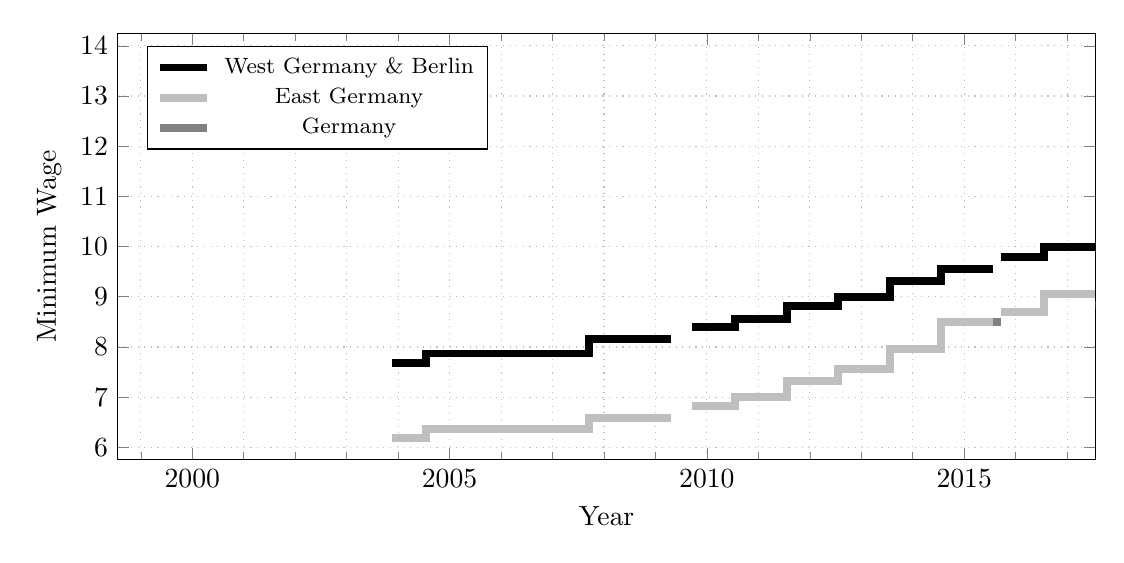
\begin{tikzpicture}

\begin{axis}[ytick={6,7,8,9,10,11,12,13,14}, height=7cm, width=14cm, grid=both, grid style = dotted, xtick={2000.45,2005.45,2010.45,2015.45},minor xtick={1999.45,2001.45,2002.45,2003.45,2004.45,2006.45,2007.45,2008.45,2009.45,2011.45,2012.45,2013.45,2014.45,2016.45,2017.45}, xlabel=Year, ylabel=Minimum Wage, ymin=5.75, ymax=14.25, xmin=1999.00, xmax=2018.00, legend pos = north west, y tick label style={/pgf/number format/.cd,fixed,fixed zerofill, precision=0,/tikz/.cd}, x tick label style={/pgf/number format/.cd,fixed,fixed zerofill, precision=0,/tikz/.cd}, legend style={font=\footnotesize}]

% West Germany and Berlin
\addplot[mark=none, solid, color=black, line width=1mm] coordinates {  (2004.33,7.68) (2005.00,7.68) (2005.00,7.87) (2008.16,7.87) (2008.16,8.15) (2009.00,8.15) (2009.75,8.15) };
\addplot[mark=none, solid, color=black, line width=1mm] coordinates {  (2010.16,8.40) (2011.00,8.40) (2011.00,8.55) (2012.00,8.55) (2012.00,8.82) (2013.00,8.82) (2013.00,9.00) (2014.00,9.00) (2014.00,9.31) (2015.00,9.31) (2015.00,9.55) (2016.00,9.55)  };
\addplot[mark=none, solid, color=black, line width=1mm] coordinates {  (2016.16,9.80) (2017.00,9.80) (2017.00,10.00) (2018.00,10.00) };
\addplot[mark=none, solid, color=black, line width=1mm] coordinates {  (2018.16,10.30) (2019.00,10.30) (2019.00,10.30) (2020.00,10.56) };

% East Germany
\addplot[mark=none, solid, color=lightgray, line width=1mm] coordinates {  (2004.33,6.18) (2005.00,6.18) (2005.00,6.36) (2008.16,6.36) (2008.16,6.58) (2009.00,6.58) (2009.75,6.58) };
\addplot[mark=none, solid, color=lightgray, line width=1mm] coordinates {  (2010.16,6.83) (2011.00,6.83) (2011.00,7.00) (2012.00,7.00) (2012.00,7.33) (2013.00,7.33) (2013.00,7.56) (2014.00,7.56) (2014.00,7.96) (2015.00,7.96) (2015.00,8.50) (2016.00,8.50)  };
\addplot[mark=none, solid, color=lightgray, line width=1mm] coordinates {  (2016.16,8.70) (2017.00,8.70) (2017.00,9.05) (2018.00,9.05) };
\addplot[mark=none, solid, color=lightgray, line width=1mm] coordinates {  (2018.16,9.55) (2019.00,9.55) (2019.00,10.05) (2020.00,10.05) };

% Germany
\addplot[mark=none, solid, color=gray, line width=1mm] coordinates {  (2016.00,8.50) (2016.16,8.50) };

\addplot[mark=none, solid, color=gray, line width=1mm] coordinates {  (2018.00,8.84) (2018.16,8.84) };

\legend{~West Germany \& Berlin,,,,~East Germany,,,,~Germany}
\end{axis}
\end{tikzpicture}
}
\end{subfigure}
\hfill
\begin{subfigure}{0.475\textwidth}
\centering
\caption{Waste Removal}
\scalebox{0.825}{
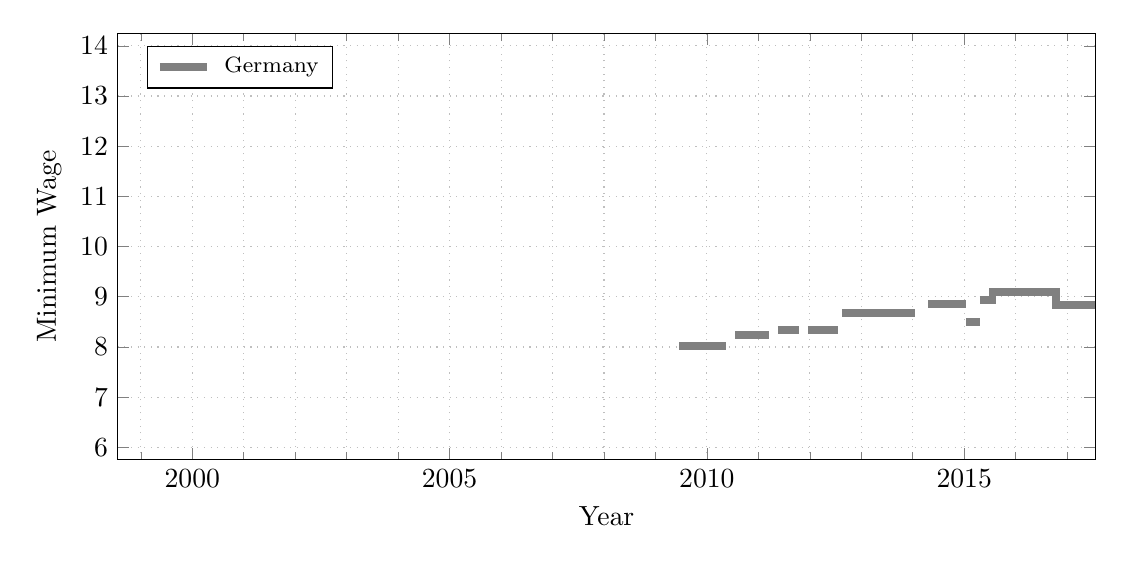
\begin{tikzpicture}

\begin{axis}[ytick={6,7,8,9,10,11,12,13,14}, height=7cm, width=14cm, grid=both, grid style = dotted, xtick={2000.45,2005.45,2010.45,2015.45},minor xtick={1999.45,2001.45,2002.45,2003.45,2004.45,2006.45,2007.45,2008.45,2009.45,2011.45,2012.45,2013.45,2014.45,2016.45,2017.45}, xlabel=Year, ylabel=Minimum Wage, ymin=5.75, ymax=14.25, xmin=1999.00, xmax=2018.00, legend pos = north west, y tick label style={/pgf/number format/.cd,fixed,fixed zerofill, precision=0,/tikz/.cd}, x tick label style={/pgf/number format/.cd,fixed,fixed zerofill, precision=0,/tikz/.cd}, legend style={font=\footnotesize}]


% Germany
\addplot[mark=none, solid, color=gray, line width=1mm] coordinates { (2009.91,8.02) (2010.83,8.02) };
\addplot[mark=none, solid, color=gray, line width=1mm] coordinates { (2011.00,8.24) (2011.66,8.24) };
\addplot[mark=none, solid, color=gray, line width=1mm] coordinates { (2011.83,8.33) (2012.24,8.33) };
\addplot[mark=none, solid, color=gray, line width=1mm] coordinates { (2012.41,8.33) (2013.00,8.33) };
\addplot[mark=none, solid, color=gray, line width=1mm] coordinates { (2013.08,8.68) (2014.49,8.68) };
\addplot[mark=none, solid, color=gray, line width=1mm] coordinates { (2014.75,8.86) (2015.49,8.86) };
\addplot[mark=none, solid, color=gray, line width=1mm] coordinates { (2015.49,8.50) (2015.75,8.50) };
\addplot[mark=none, solid, color=gray, line width=1mm] coordinates { (2015.75,8.94) (2016.00,8.94) (2016.00,9.10) (2017.24,9.10) (2017.24,8.84) (2018.00,8.84) }; % (2018.00,8.84) (2019.00,8.84) (2019.00,9.19) (2020.00,9.19)



\legend{~Germany,,,,,,}

\end{axis}
\end{tikzpicture}
}
\end{subfigure}
\vskip \baselineskip
\begin{subfigure}{0.475\textwidth}
\centering
\caption{Nursing Care}
\scalebox{0.825}{
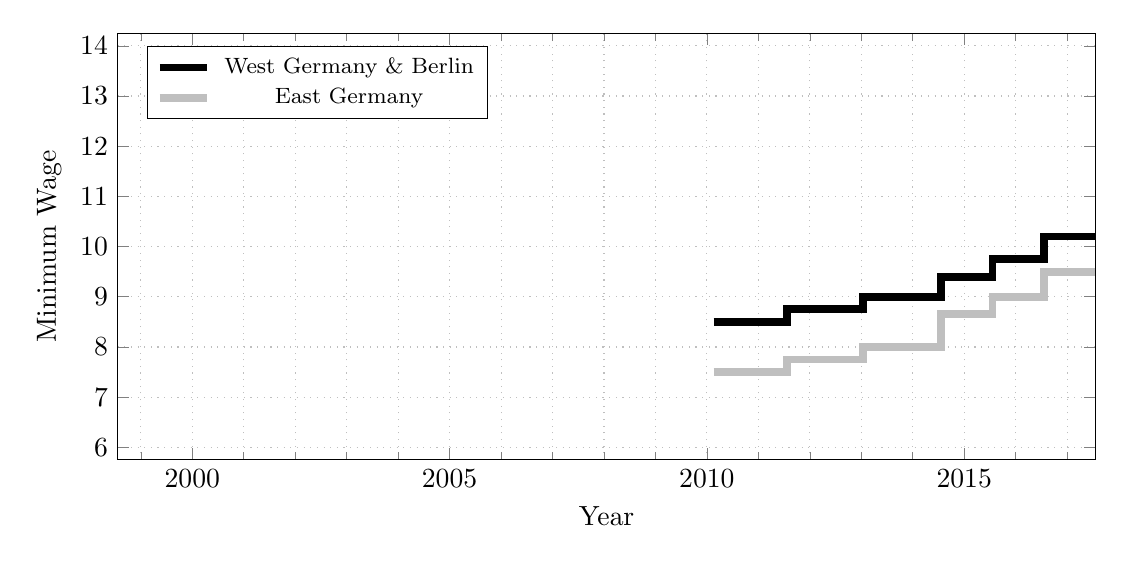
\begin{tikzpicture}

\begin{axis}[ytick={6,7,8,9,10,11,12,13,14}, height=7cm, width=14cm, grid=both, grid style = dotted, xtick={2000.45,2005.45,2010.45,2015.45},minor xtick={1999.45,2001.45,2002.45,2003.45,2004.45,2006.45,2007.45,2008.45,2009.45,2011.45,2012.45,2013.45,2014.45,2016.45,2017.45}, xlabel=Year, ylabel=Minimum Wage, ymin=5.75, ymax=14.25, xmin=1999.00, xmax=2018.00, legend pos = north west, y tick label style={/pgf/number format/.cd,fixed,fixed zerofill, precision=0,/tikz/.cd}, x tick label style={/pgf/number format/.cd,fixed,fixed zerofill, precision=0,/tikz/.cd}, legend style={font=\footnotesize}]

% West Germany and Berlin
\addplot[mark=none, solid, color=black, line width=1mm] coordinates {  (2010.58,8.50) (2012.00,8.50) (2012.00,8.75)  (2013.49,8.75) (2013.49,9.00) (2015.00,9.00) (2015.00,9.40) (2016.00,9.40) (2016.00,9.75)  (2017.00,9.75) (2017.00,10.20)  (2018.00,10.20) }; % (2018.00,10.55) (2019.00,10.55) (2019.00,11.05)  (2020.00,11.05)

% East Germany
\addplot[mark=none, solid, color=lightgray, line width=1mm] coordinates {  (2010.58,7.50) (2012.00,7.50) (2012.00,7.75)  (2013.49,7.75) (2013.49,8.00) (2015.00,8.00) (2015.00,8.65) (2016.00,8.65) (2016.00,9.00)  (2017.00,9.00) (2017.00,9.50)  (2018.00,9.50)  }; % (2018.00,10.05) (2019.00,10.05) (2019.00,10.55)  (2020.00,10.55)


\legend{~West Germany \& Berlin,~East Germany}

\end{axis}
\end{tikzpicture}
}
\end{subfigure}
\hfill
\begin{subfigure}{0.475\textwidth}
\centering
\caption{Security}
\scalebox{0.825}{
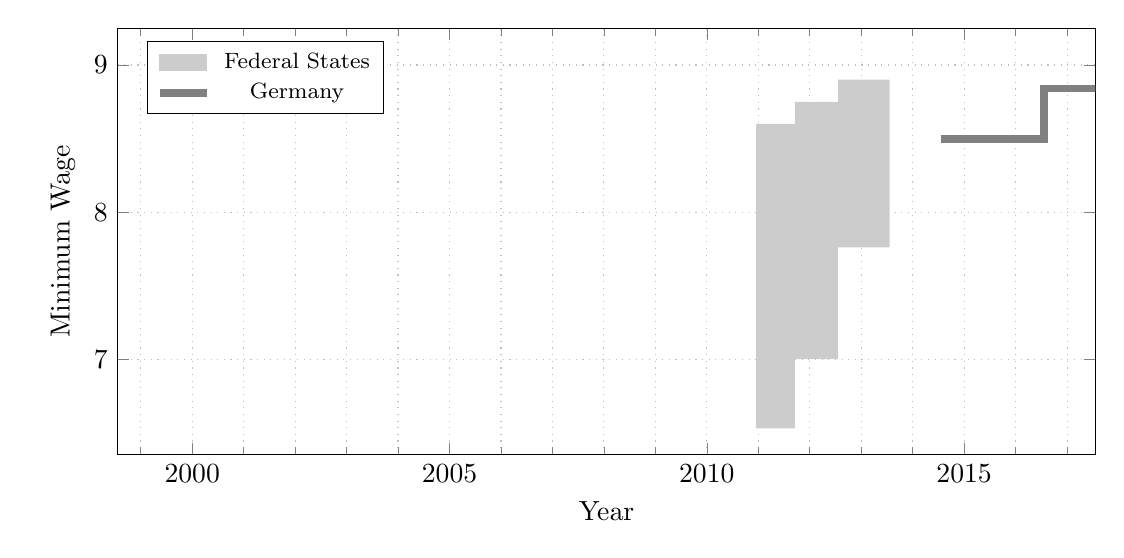
\begin{tikzpicture}

\begin{axis}[ytick={6,7,8,9,10}, height=7cm, width=14cm, grid=both, grid style = dotted, xtick={2000.45,2005.45,2010.45,2015.45},minor xtick={1999.45,2001.45,2002.45,2003.45,2004.45,2006.45,2007.45,2008.45,2009.45,2011.45,2012.45,2013.45,2014.45,2016.45,2017.45}, xlabel=Year, ylabel=Minimum Wage\vphantom{{\LARGE I}}, ymin=6.35, ymax=9.25, xmin=1999.00, xmax=2018.00, legend pos = north west, y tick label style={/pgf/number format/.cd,fixed,fixed zerofill, precision=0,/tikz/.cd}, x tick label style={/pgf/number format/.cd,fixed,fixed zerofill, precision=0,/tikz/.cd}, legend style={font=\footnotesize}]

% upper limit on minimum wages by federal states
\addplot[name path = A, draw=none] coordinates {  (2011.41,8.60) (2012.16,8.60) (2012.16,8.75) (2013.00,8.75) (2013.00,8.90) (2014.00,8.90)  };

% lower limit on minimum wages by federal states
\addplot[name path = B, draw=none] coordinates {  (2011.41,6.53) (2012.16,6.53) (2012.16,7.00) (2013.00,7.00) (2013.00,7.76) (2014.00,7.76) };

\addplot[color=gray!40!white] fill between[of=A and B];

% Baden-Wuerttemberg
%\addplot[mark=none, solid, color=black!100!white, line width=1mm] coordinates {  (2011.41,8.60) (2012.16,8.60) (2012.16,8.75) (2013.00,8.75) (2013.00,8.90) (2014.00,8.90)  };

% Bavaria
%\addplot[mark=none, solid, color=black!50!white, line width=1mm] coordinates {  (2011.41,8.14) (2012.16,8.14) (2012.16,8.28) (2013.00,8.28) (2013.00,8.42) (2014.00,8.42)  };

% North-Rhine Westphalia
%\addplot[mark=none, solid, color=black!90!white, line width=1mm] coordinates {  (2011.41,7.95) (2012.16,7.95) (2012.16,8.09) (2013.00,8.09) (2013.00,8.23) (2014.00,8.23)  };

% Hesse
%\addplot[mark=none, solid, color=black!40!white, line width=1mm] coordinates {  (2011.41,7.50) (2012.16,7.50) (2012.16,7.63) (2013.00,7.63) (2013.00,7.76) (2014.00,7.76)  };

% Lower Saxony
%\addplot[mark=none, solid, color=black!80!white, line width=1mm] coordinates {  (2011.41,7.26) (2012.16,7.26) (2012.16,7.38) (2013.00,7.38) };

% Bremen
%\addplot[mark=none, solid, color=black!30!white, line width=1mm] coordinates {  (2011.41,7.16) (2012.16,7.16) (2012.16,7.33) (2013.00,7.33)};

% Hamburg
%\addplot[mark=none, solid, color=black!70!white, line width=1mm] coordinates {  (2011.41,7.12) (2012.16,7.12) (2012.16,7.31) (2013.00,7.31) };

% Other Federal States
%\addplot[mark=none, solid, color=black!20!white, line width=1mm] coordinates {  (2011.41,6.53) (2012.16,6.53) (2012.16,7.00) (2013.00,7.00)  };

% Other Federal States + Lower Saxony + Bremen + Hamburg
%\addplot[mark=none, solid, color=black!60!white, line width=1mm] coordinates {  (2013.00,7.50) (2014.00,7.50) };

% Germany
\addplot[mark=none, solid, color=gray, line width=1mm] coordinates {  (2015.00,8.50) (2017.00,8.50) (2017.00,8.84) (2018.00,8.84) (2019.00,8.84) (2019.00,9.19) (2020.00,9.19) };

%\legend{BW,BY,NW,HE,NI,HB,HH,BB/BE/MV/RP/SH/SL/SN/ST/TH,\shortstack{BB/BE/HB/HH/MV/NI/... \\ .../RP/SH/SL/SN/ST/TH},Germany}
\legend{,,~Federal States,~Germany}

\end{axis}
\end{tikzpicture}
}
\end{subfigure}
\vspace*{-0.3cm}
\floatfoot{ \footnotesize \textsc{Note. ---} The figures show the level of sectoral minimum wages (in Euro per hour) between 1999 and 2017. The ticks on the x axes refer to 30 June of the respective year. Line interruptions point to periods in which no minimum wage was in force. In the security sector for the years 2011-2013, minimum wages vary by federal state. The grey shade indicates the range of federal minimum wage regulations in this sector.  AEntG = Arbeitnehmerentsendegesetz. AÜG = Arbeitnehmerüberlassungsgesetz. MiLoG = Mindestlohngesetz. TVG = Tarifvertragsgesetz. Sources: AEntG $\plus$ AÜG $\plus$ Bundesanzeiger $\plus$ MiLoG $\plus$ TVG. }
\end{figure}



\clearpage



\begin{figure}[!ht]
\addtocounter{figure}{-1}
\centering
\caption{Variation in Sectoral Minimum Wages (Cont.)}
%\label{fig:B4}
\begin{subfigure}{0.475\textwidth}
\addtocounter{subfigure}{8}
\centering
\caption{Temporary Work}
\scalebox{0.825}{
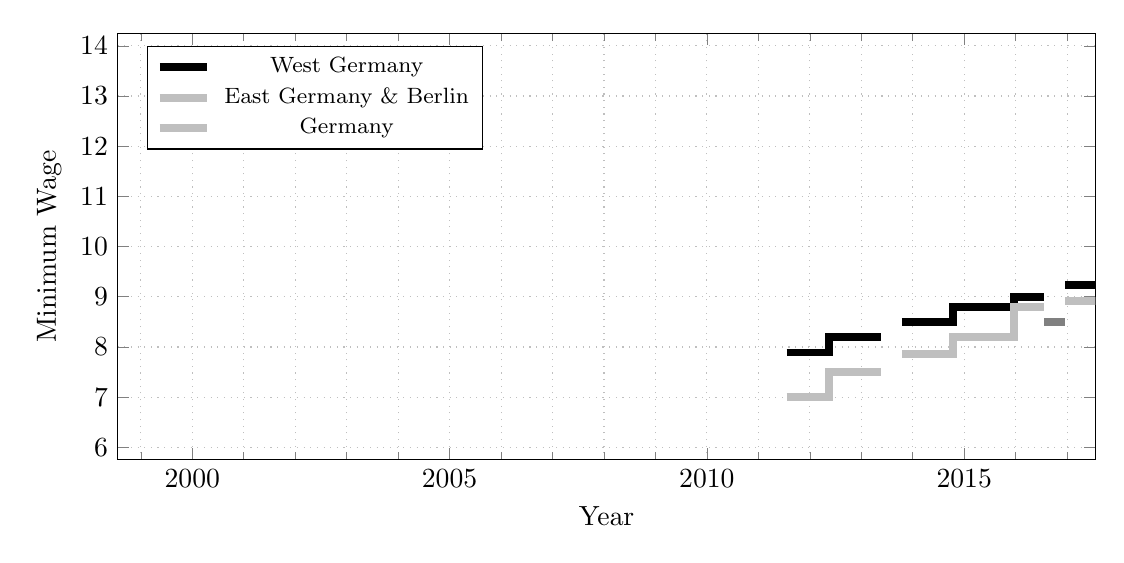
\begin{tikzpicture}

\begin{axis}[ytick={6,7,8,9,10,11,12,13,14}, height=7cm, width=14cm, grid=both, grid style = dotted, xtick={2000.45,2005.45,2010.45,2015.45},minor xtick={1999.45,2001.45,2002.45,2003.45,2004.45,2006.45,2007.45,2008.45,2009.45,2011.45,2012.45,2013.45,2014.45,2016.45,2017.45}, xlabel=Year, ylabel=Minimum Wage, ymin=5.75, ymax=14.25, xmin=1999.00, xmax=2018.00, legend pos = north west, y tick label style={/pgf/number format/.cd,fixed,fixed zerofill, precision=0,/tikz/.cd}, x tick label style={/pgf/number format/.cd,fixed,fixed zerofill, precision=0,/tikz/.cd}, legend style={font=\footnotesize}]

% West Germany
\addplot[mark=none, solid, color=black, line width=1mm] coordinates { (2012.00,7.89) (2012.83,7.89) (2012.83,8.19) (2013.83,8.19) };
\addplot[mark=none, solid, color=black, line width=1mm] coordinates { (2014.24,8.50) (2015.24,8.50) (2015.24,8.80) (2016.41,8.80) (2016.41,9.00) (2017.00,9.00)  };
\addplot[mark=none, solid, color=black, line width=1mm] coordinates { (2017.41,9.23) (2018.24,9.23) (2018.24,9.49) (2019.00,9.49) };
\addplot[mark=none, solid, color=black, line width=1mm] coordinates { (2019.24,9.79) (2019.75,9.79) (2019.75,9.96) (2020,9.96)  };



% East Germany and Berlin
\addplot[mark=none, solid, color=lightgray, line width=1mm] coordinates { (2012.00,7.01) (2012.83,7.01) (2012.83,7.50) (2013.83,7.50) };
\addplot[mark=none, solid, color=lightgray, line width=1mm] coordinates { (2014.24,7.86) (2015.24,7.86) (2015.24,8.20) (2016.41,8.20) (2016.41,8.80) (2017.00,8.80)  };
\addplot[mark=none, solid, color=lightgray, line width=1mm] coordinates { (2017.41,8.91) (2018.24,8.91) (2018.24,9.27) (2019.00,9.27)   };
\addplot[mark=none, solid, color=lightgray, line width=1mm] coordinates { (2019.24,9.49) (2019.75,9.49) (2019.75,9.66) (2020,9.66)  };

% Germany
\addplot[mark=none, solid, color=gray, line width=1mm] coordinates { (2017.00,8.50) (2017.41,8.50) };
\addplot[mark=none, solid, color=gray, line width=1mm] coordinates { (2019.00,9.49) (2019.24,9.49) };


\legend{~West Germany,,,,~East Germany \& Berlin,,,~Germany,}
\end{axis}
\end{tikzpicture}
}
\end{subfigure}
\hfill
\begin{subfigure}{0.475\textwidth}
\centering
\caption{Scaffolding}
\scalebox{0.825}{
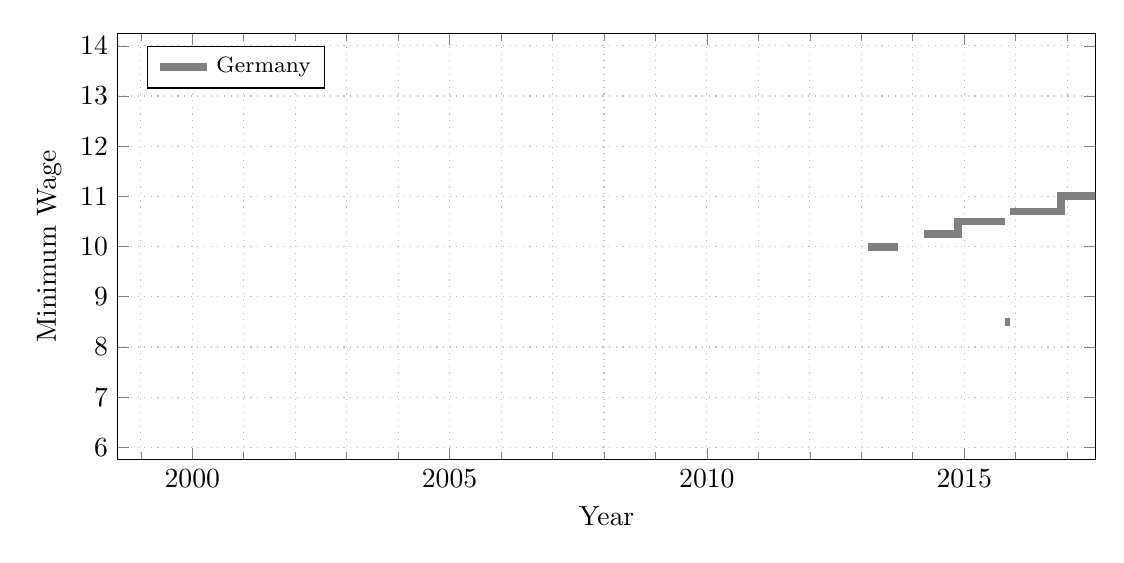
\begin{tikzpicture}

\begin{axis}[ytick={6,7,8,9,10,11,12,13,14}, height=7cm, width=14cm, grid=both, grid style = dotted, xtick={2000.45,2005.45,2010.45,2015.45},minor xtick={1999.45,2001.45,2002.45,2003.45,2004.45,2006.45,2007.45,2008.45,2009.45,2011.45,2012.45,2013.45,2014.45,2016.45,2017.45}, xlabel=Year, ylabel=Minimum Wage, ymin=5.75, ymax=14.25, xmin=1999.00, xmax=2018.00, legend pos = north west, y tick label style={/pgf/number format/.cd,fixed,fixed zerofill, precision=0,/tikz/.cd}, x tick label style={/pgf/number format/.cd,fixed,fixed zerofill, precision=0,/tikz/.cd}, legend style={font=\footnotesize}]

% Germany
\addplot[mark=none, solid, color=gray, line width=1mm] coordinates { (2013.58,10.00) (2014.16,10.00) };
\addplot[mark=none, solid, color=gray, line width=1mm] coordinates { (2014.66,10.25) (2015.33,10.25) (2015.33,10.50) (2016.24,10.50)};
\addplot[mark=none, solid, color=gray, line width=1mm] coordinates { (2016.24,8.50) (2016.33,8.50) };
\addplot[mark=none, solid, color=gray, line width=1mm] coordinates { (2016.33,10.70)  (2017.33,10.70) (2017.33,11.00) (2018.33,11.00) (2018.33,8.84) (2018.49,8.84) (2018.49,11.35) (2019.41,11.35) (2019.41,9.19) (2019.49,9.19) (2019.49,11.88) (2020.00,11.88) };


\legend{Germany,}

\end{axis}
\end{tikzpicture}
}
\end{subfigure}
\vskip \baselineskip
\begin{subfigure}{0.475\textwidth}
\centering
\caption{Stonemasonry}
\scalebox{0.825}{
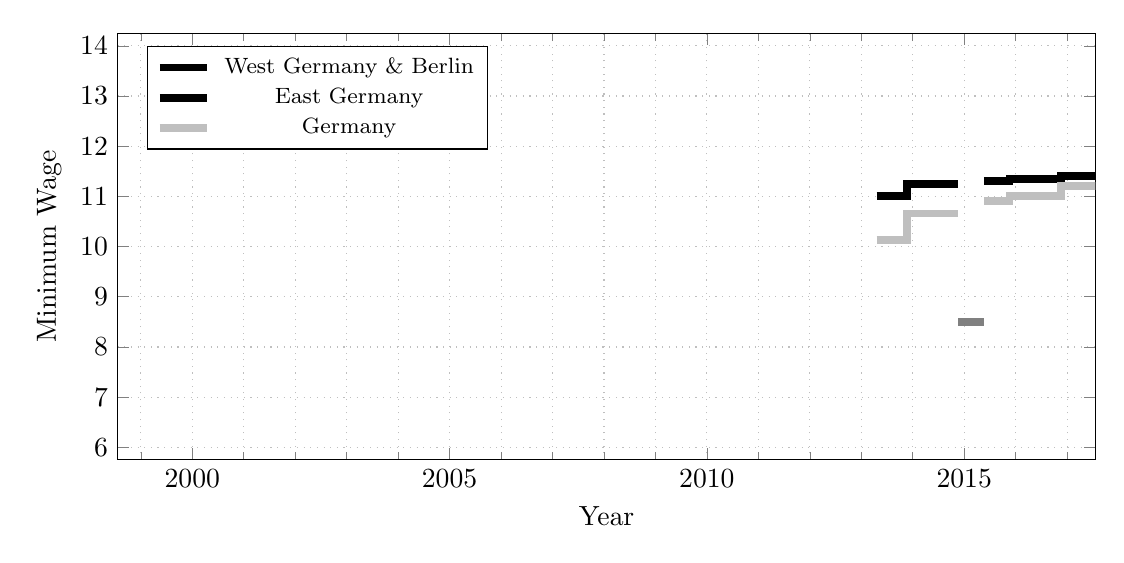
\begin{tikzpicture}

\begin{axis}[ytick={6,7,8,9,10,11,12,13,14}, height=7cm, width=14cm, grid=both, grid style = dotted, xtick={2000.45,2005.45,2010.45,2015.45},minor xtick={1999.45,2001.45,2002.45,2003.45,2004.45,2006.45,2007.45,2008.45,2009.45,2011.45,2012.45,2013.45,2014.45,2016.45,2017.45}, xlabel=Year, ylabel=Minimum Wage, ymin=5.75, ymax=14.25, xmin=1999.00, xmax=2018.00, legend pos = north west, y tick label style={/pgf/number format/.cd,fixed,fixed zerofill, precision=0,/tikz/.cd}, x tick label style={/pgf/number format/.cd,fixed,fixed zerofill, precision=0,/tikz/.cd}, legend style={font=\footnotesize}]


% West Germany and Berlin
\addplot[mark=none, solid, color=black, line width=1mm] coordinates { (2013.75,11.00) (2014.33,11.00) (2014.33,11.25)  (2015.33,11.25) };
\addplot[mark=none, solid, color=black, line width=1mm] coordinates { (2015.83,11.30) (2016.33,11.30) (2016.33,11.35) (2017.33,11.35) (2017.33,11.40)  (2018.33,11.40) };

% East Germany
\addplot[mark=none, solid, color=lightgray, line width=1mm] coordinates { (2013.75,10.13) (2014.33,10.13) (2014.33,10.66)  (2015.33,10.66) };
\addplot[mark=none, solid, color=lightgray, line width=1mm] coordinates { (2015.83,10.90) (2016.33,10.90) (2016.33,11.00) (2017.33,11.00) (2017.33,11.20)  (2018.33,11.20) };

% Germany
\addplot[mark=none, solid, color=gray, line width=1mm] coordinates { (2015.33,8.50) (2015.83,8.50)  };
\addplot[mark=none, solid, color=gray, line width=1mm] coordinates { (2018.33,11.40) (2019.33,11.40) (2019.33,9.19) (2019.66,9.19) (2019.66,11.85) (2020.00,11.85) };


\legend{~West Germany \& Berlin,~East Germany,~Germany,}

\end{axis}
\end{tikzpicture}
}
\end{subfigure}
\hfill
\begin{subfigure}{0.475\textwidth}
\centering
\caption{Hairdressing}
\scalebox{0.825}{
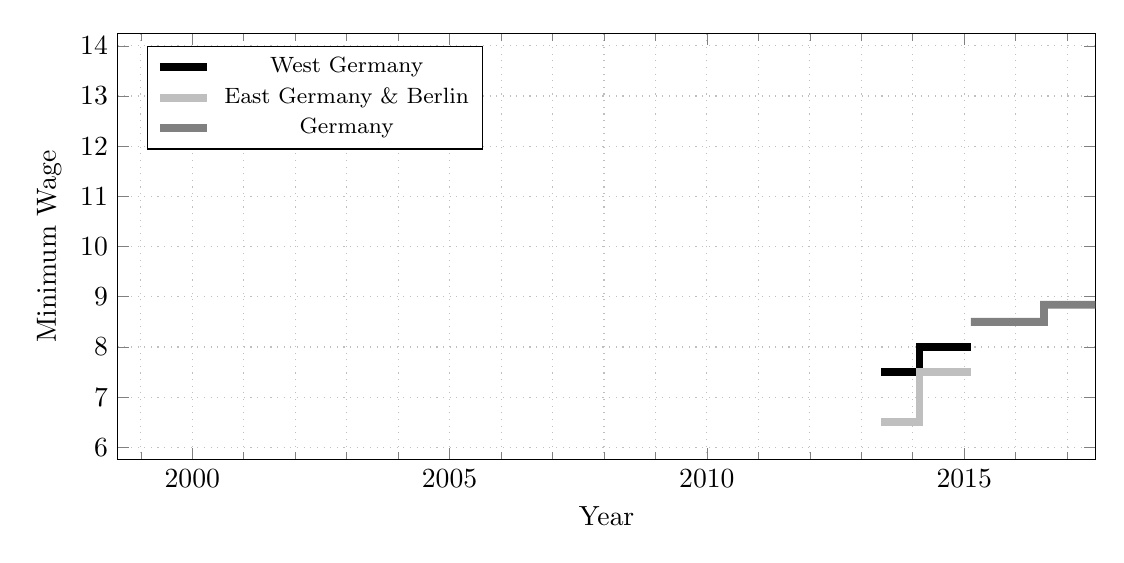
\begin{tikzpicture}

\begin{axis}[ytick={6,7,8,9,10,11,12,13,14}, height=7cm, width=14cm, grid=both, grid style = dotted, xtick={2000.45,2005.45,2010.45,2015.45},minor xtick={1999.45,2001.45,2002.45,2003.45,2004.45,2006.45,2007.45,2008.45,2009.45,2011.45,2012.45,2013.45,2014.45,2016.45,2017.45}, xlabel=Year, ylabel=Minimum Wage, ymin=5.75, ymax=14.25, xmin=1999.00, xmax=2018.00, legend pos = north west, y tick label style={/pgf/number format/.cd,fixed,fixed zerofill, precision=0,/tikz/.cd}, x tick label style={/pgf/number format/.cd,fixed,fixed zerofill, precision=0,/tikz/.cd}, legend style={font=\footnotesize}]

% West Germany
\addplot[mark=none, solid, color=black, line width=1mm] coordinates {  (2013.83,7.50) (2014.58,7.50) (2014.58,8.00) (2015.58,8.00) };

% East Germany and Berlin
\addplot[mark=none, solid, color=lightgray, line width=1mm] coordinates { (2013.83,6.50) (2014.58,6.50) (2014.58,7.50) (2015.58,7.50) };

% Germany
\addplot[mark=none, solid, color=gray, line width=1mm] coordinates {  (2015.58,8.50) (2017.00,8.50) (2017.00,8.84) (2019.00,8.84) (2019.00,9.91) (2020.00,9.19) };


\legend{~West Germany,~East Germany \& Berlin,~Germany}
\end{axis}
\end{tikzpicture}
}
\end{subfigure}


\floatfoot{ \footnotesize \textsc{Note. ---} The figures show the level of sectoral minimum wages (in Euro per hour) between 1999 and 2017. The ticks on the x axes refer to 30 June of the respective year. Line interruptions point to periods in which no minimum wage was in force. AEntG = Arbeitnehmerentsendegesetz. AÜG = Arbeitnehmerüberlassungsgesetz. MiLoG = Mindestlohngesetz. TVG = Tarifvertragsgesetz. Sources: AEntG $\plus$ AÜG $\plus$ Bundesanzeiger $\plus$ MiLoG $\plus$ TVG.}
\end{figure}

\clearpage



\begin{figure}[!ht]
\addtocounter{figure}{-1}
\centering
\caption{Variation in Sectoral Minimum Wages (Cont.)}
%\label{fig:B4}
\begin{subfigure}{0.475\textwidth}
\addtocounter{subfigure}{12}
\centering
\caption{Chimney Sweeping}
\scalebox{0.825}{
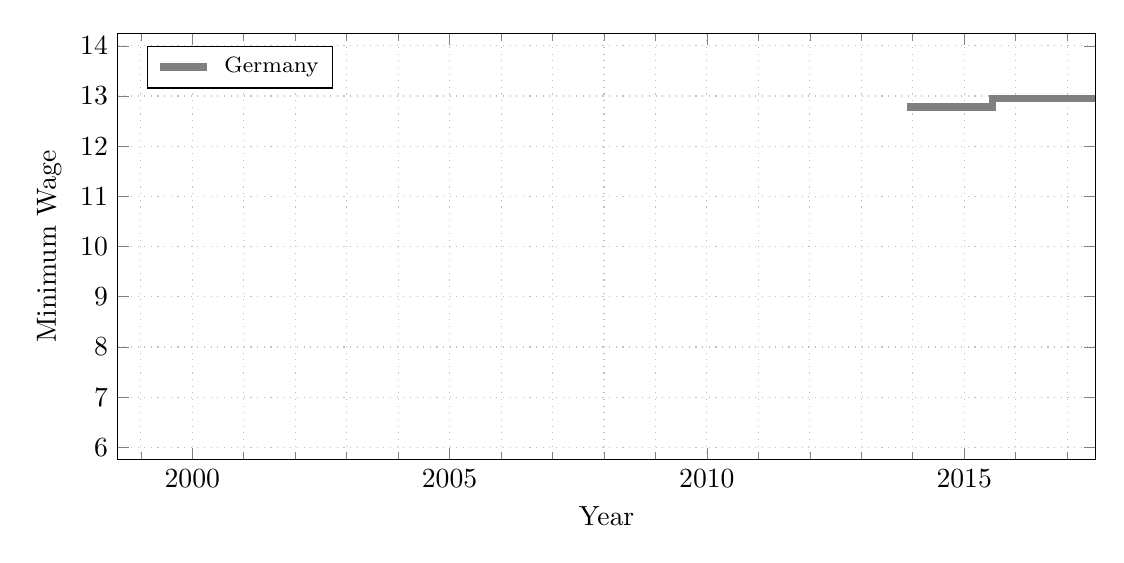
\begin{tikzpicture}

\begin{axis}[ytick={6,7,8,9,10,11,12,13,14}, height=7cm, width=14cm, grid=both, grid style = dotted, xtick={2000.45,2005.45,2010.45,2015.45},minor xtick={1999.45,2001.45,2002.45,2003.45,2004.45,2006.45,2007.45,2008.45,2009.45,2011.45,2012.45,2013.45,2014.45,2016.45,2017.45}, xlabel=Year, ylabel=Minimum Wage, ymin=5.75, ymax=14.25, xmin=1999.00, xmax=2018.00, legend pos = north west, y tick label style={/pgf/number format/.cd,fixed,fixed zerofill, precision=0,/tikz/.cd}, x tick label style={/pgf/number format/.cd,fixed,fixed zerofill, precision=0,/tikz/.cd}, legend style={font=\footnotesize}]

% Germany
\addplot[mark=none, solid, color=gray, line width=1mm] coordinates {  (2014.33,12.78) (2016.00,12.78) (2016.00,12.95) (2018.00,12.95)  }; % (2018.00,8.84) (2018.75,8.84) (2018.75,13.20) (2020.00,13.20)


\legend{~Germany}

\end{axis}
\end{tikzpicture}
}
\end{subfigure}
\hfill
\begin{subfigure}{0.475\textwidth}
\centering
\caption{Slaughtering \& Meat Processing}
\scalebox{0.825}{
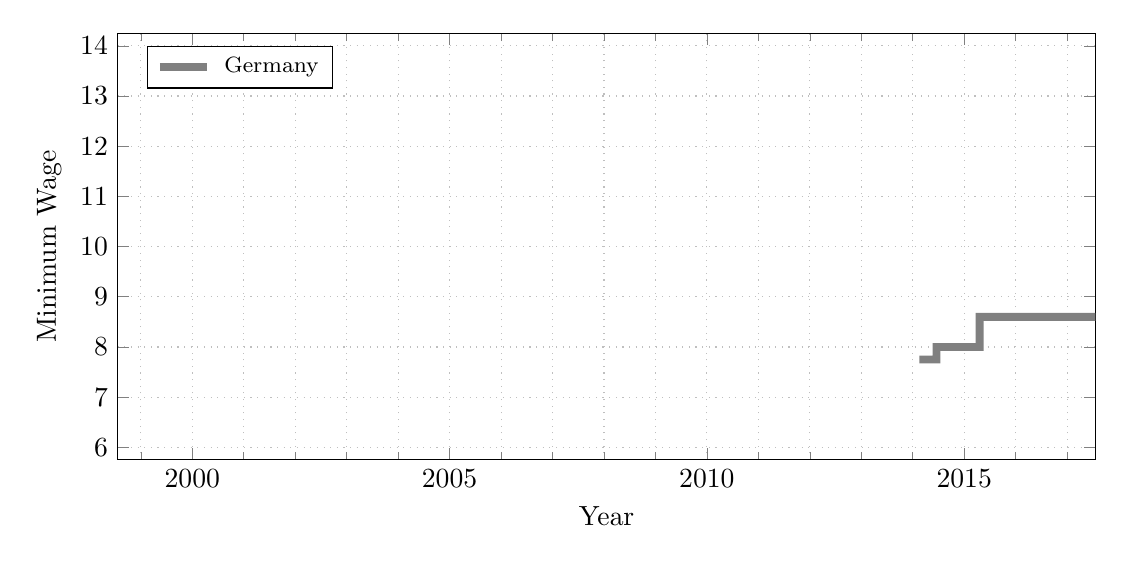
\begin{tikzpicture}

\begin{axis}[ytick={6,7,8,9,10,11,12,13,14}, height=7cm, width=14cm, grid=both, grid style = dotted, xtick={2000.45,2005.45,2010.45,2015.45},minor xtick={1999.45,2001.45,2002.45,2003.45,2004.45,2006.45,2007.45,2008.45,2009.45,2011.45,2012.45,2013.45,2014.45,2016.45,2017.45}, xlabel=Year, ylabel=Minimum Wage, ymin=5.75, ymax=14.25, xmin=1999.00, xmax=2018.00, legend pos = north west, y tick label style={/pgf/number format/.cd,fixed,fixed zerofill, precision=0,/tikz/.cd}, x tick label style={/pgf/number format/.cd,fixed,fixed zerofill, precision=0,/tikz/.cd}, legend style={font=\footnotesize}]

% Germany
\addplot[mark=none, solid, color=gray, line width=1mm] coordinates {  (2014.58,7.75) (2014.91,7.75)  (2014.91,8.00) (2015.75,8.00) (2015.75,8.60) (2016.91,8.60)  (2018.00,8.60) (2019.00,8.84) (2019.00,8.91) (2019.00,9.19) };

\legend{~Germany}

\end{axis}
\end{tikzpicture}
}
\end{subfigure}
\vskip \baselineskip
\begin{subfigure}{0.475\textwidth}
\centering
\caption{Textile \& Clothing}
\scalebox{0.825}{
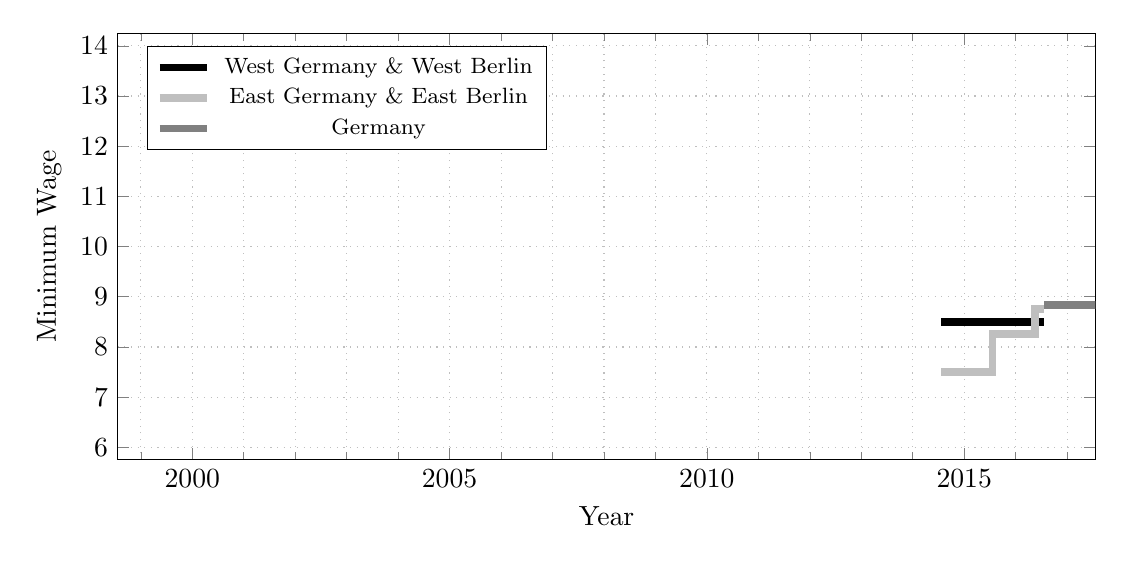
\begin{tikzpicture}

\begin{axis}[ytick={6,7,8,9,10,11,12,13,14}, height=7cm, width=14cm, grid=both, grid style = dotted, xtick={2000.45,2005.45,2010.45,2015.45},minor xtick={1999.45,2001.45,2002.45,2003.45,2004.45,2006.45,2007.45,2008.45,2009.45,2011.45,2012.45,2013.45,2014.45,2016.45,2017.45}, xlabel=Year, ylabel=Minimum Wage, ymin=5.75, ymax=14.25, xmin=1999.00, xmax=2018.00, legend pos = north west, y tick label style={/pgf/number format/.cd,fixed,fixed zerofill, precision=0,/tikz/.cd}, x tick label style={/pgf/number format/.cd,fixed,fixed zerofill, precision=0,/tikz/.cd}, legend style={font=\footnotesize}]

% West Germany and Berlin
\addplot[mark=none, solid, color=black, line width=1mm] coordinates { (2015.00,8.50) (2016.00,8.50) (2016.83,8.50) (2017.00,8.50) };

% East Germany
\addplot[mark=none, solid, color=lightgray, line width=1mm] coordinates { (2015.00,7.50) (2016.00,7.50) (2016.00,8.25) (2016.83,8.25) (2016.83,8.75) (2017.00,8.75) };

% Germany
\addplot[mark=none, solid, color=gray, line width=1mm] coordinates { (2017.00,8.84) (2019.00,8.84) (2019.00,9.19) (2020.00,9.19)  };


\legend{~West Germany \& West Berlin,~East Germany \& East Berlin,~Germany}
\end{axis}
\end{tikzpicture}
}
\end{subfigure}
\hfill
\begin{subfigure}{0.475\textwidth}
\centering
\caption{Agriculture, Forestry \& Gardening}
\scalebox{0.825}{
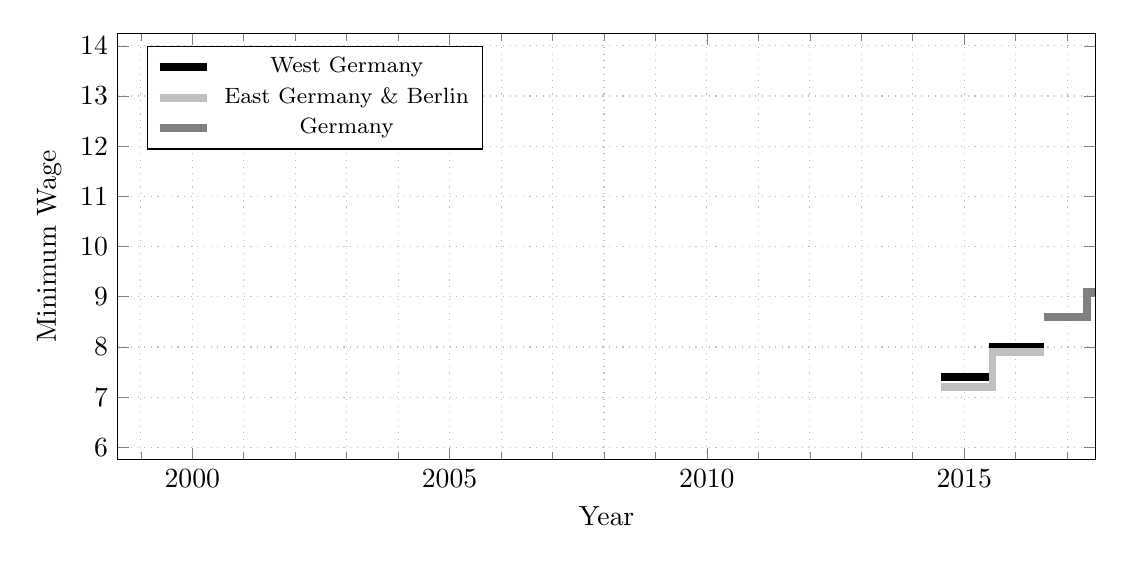
\begin{tikzpicture}

\begin{axis}[ytick={6,7,8,9,10,11,12,13,14}, height=7cm, width=14cm, grid=both, grid style = dotted, xtick={2000.45,2005.45,2010.45,2015.45},minor xtick={1999.45,2001.45,2002.45,2003.45,2004.45,2006.45,2007.45,2008.45,2009.45,2011.45,2012.45,2013.45,2014.45,2016.45,2017.45}, xlabel=Year, ylabel=Minimum Wage, ymin=5.75, ymax=14.25, xmin=1999.00, xmax=2018.00, legend pos = north west, y tick label style={/pgf/number format/.cd,fixed,fixed zerofill, precision=0,/tikz/.cd}, x tick label style={/pgf/number format/.cd,fixed,fixed zerofill, precision=0,/tikz/.cd}, legend style={font=\footnotesize}]

% West Germany
\addplot[mark=none, solid, color=black, line width=1mm] coordinates {  (2015.00,7.40) (2016.00,7.40) (2016.00,8.00) (2017.00,8.00) };

% East Germany and Berlin
\addplot[mark=none, solid, color=lightgray, line width=1mm] coordinates { (2015.00,7.20) (2016.00,7.20) (2016.00,7.90) (2017.00,7.90) };

% Germany
\addplot[mark=none, solid, color=gray, line width=1mm] coordinates { (2017.00,8.60) (2017.83,8.60) (2017.83,9.10) (2018.00,9.10)  }; % (2018.00,8.84) (2019.00,8.84) (2019.00,9.19)  (2020.00,9.19)


\legend{~West Germany,~East Germany \& Berlin,~Germany}
\end{axis}
\end{tikzpicture}
}
\end{subfigure}


\floatfoot{ \footnotesize \textsc{Note. ---} The figures show the level of sectoral minimum wages (in Euro per hour) between 1999 and 2017. The ticks on the x axes refer to 30 June of the respective year. Line interruptions point to periods in which no minimum wage was in force. AEntG = Arbeitnehmerentsendegesetz. AÜG = Arbeitnehmerüberlassungsgesetz. MiLoG = Mindestlohngesetz. TVG = Tarifvertragsgesetz. Sources: AEntG $\plus$ AÜG $\plus$ Bundesanzeiger $\plus$ MiLoG $\plus$ TVG.}
\end{figure}


\end{landscape}








\clearpage



\begin{landscape}

\section{Appendix: Labor Market Concentration}
\label{sec:C}
\setcounter{table}{0} % reset table counter
\setcounter{figure}{0} % reset figure counter

%\vspace*{-0.7cm}

\begin{table}[!ht]

\centering

\renewcommand{\arraystretch}{1.5}
\scalebox{0.85}{

\begin{threeparttable}
\caption{Empirical Literature on Labor Market Concentration}
\label{tab:C1}
%\vspace{-0.1cm}
\begin{tabular}[c]{|C{5.25cm}|C{3.75cm}C{4.25cm}:C{5cm}:C{2.75cm}C{2.5cm}C{2.5cm}|} \hline \hline



\multirow{2}{*}{\diagbox[height=3\line, innerwidth=5.25cm]{Study}{Dimension}} & \multirow{2.4}{*}{Index}   & \multirow{2.4}{*}{Object} & \multirow{2.4}{*}{\shortstack{Labor Market Definition\vphantom{y}: \\ Work $\times$ Space}} & \multirow{2.4}{*}{Source}  & \multirow{2.4}{*}{Country} & \multirow{2.4}{*}{Year} \\

&&&&&& \\ \hline
		
\multirow{1}{*}{\citet{AbelEtAl2018}} &  \multirow{1}{*}{HHI}   &  \multirow{1}{*}{employment} &  \multirow{1}{*}{SIC-2 $\times$ NUTS-2} &   \multirow{1}{*}{NES-ASHE}  &  \multirow{1}{*}{UK} &  \multirow{1}{*}{1998-2017} \\ \hdashline % (1)


\multirow{1}{*}{\citet{Arnold2020}} &  \multirow{1}{*}{flow-adjusted HHI}   &  \multirow{1}{*}{employment} &  \multirow{1}{*}{NAICS-4 $\times$ CZ} &   \multirow{1}{*}{LBD}  &  \multirow{1}{*}{USA} &  \multirow{1}{*}{1995-2014} \\ \hdashline % (100)


\multirow{1}{*}{\citet{AzarEtAl2017}} &  \multirow{1}{*}{HHI}   &  \multirow{1}{*}{vacancies/applications} &  \multirow{1}{*}{SOC-6 $\times$ CZ} &   \multirow{1}{*}{CareerBuilder}  &  \multirow{1}{*}{USA} &  \multirow{1}{*}{2010-2013} \\ \hdashline % (35)

\multirow{1}{*}{\citet{AzarEtAl2019a}} &  \multirow{1}{*}{HHI}   &  \multirow{1}{*}{vacancies} &  \multirow{1}{*}{SOC-6 $\times$ county} &   \multirow{1}{*}{BGT}  &  \multirow{1}{*}{USA} &  \multirow{1}{*}{2010-2016} \\ \hdashline % (80-85)

\multirow{1}{*}{\citet{AzarEtAl2019b}} &  \multirow{1}{*}{HHI}   &  \multirow{1}{*}{vacancies} &  \multirow{1}{*}{SOC-6 $\times$ CZ} &   \multirow{1}{*}{CareerBuilder}  &  \multirow{1}{*}{USA} &  \multirow{1}{*}{2010-2013} \\ \hdashline % (35)

\multirow{1}{*}{\citet{AzarEtAl2020})} &  \multirow{1}{*}{HHI}   &  \multirow{1}{*}{vacancies} &  \multirow{1}{*}{SOC-6 $\times$ CZ} &   \multirow{1}{*}{BGT}  &  \multirow{1}{*}{USA} &  \multirow{1}{*}{2016} \\ \hdashline % (80-85)

\multirow{1}{*}{\citet{BassaniniEtAl2019}} &  \multirow{1}{*}{HHI}   &  \multirow{1}{*}{employment/hires} &  \multirow{1}{*}{ISCO-4 $\times$ CZ} &   \multirow{1}{*}{DADS}  &  \multirow{1}{*}{France} &  \multirow{1}{*}{2009-2012} \\ \hdashline % (100)

\multirow{1}{*}{\citet{BassierEtAl2021}} &  \multirow{1}{*}{HHI}   &  \multirow{1}{*}{employment} &  \multirow{1}{*}{NAICS-4 $\times$ CZ} &   \multirow{1}{*}{OMI}  &  \multirow{1}{*}{USA} &  \multirow{1}{*}{2000-2017} \\ \hdashline

\multirow{1}{*}{\citet{BergerEtAl2019}} &  \multirow{1}{*}{HHI}   &  \multirow{1}{*}{employment/wages} &  \multirow{1}{*}{NAICS-3 $\times$ CZ} &   \multirow{1}{*}{LBD}  &  \multirow{1}{*}{USA} &  \multirow{1}{*}{1976/2014} \\ \hdashline % (100)

%\multirow{1}{*}{\citet{Beck1993}} &  \multirow{1}{*}{HHI}   &  \multirow{1}{*}{employment} &  \multirow{1}{*}{25 miles radius (only teachers)} &   \multirow{1}{*}{MO Schools}  &  \multirow{1}{*}{USA} &  \multirow{1}{*}{1982-1990} \\ \hdashline % (100)


\multirow{1}{*}{\citet{BenmelechEtAl2020}} &  \multirow{1}{*}{HHI}   &  \multirow{1}{*}{employment} &  \multirow{1}{*}{SIC-3/4 $\times$ county} &   \multirow{1}{*}{LBD}  &  \multirow{1}{*}{USA} &  \multirow{1}{*}{1977-2009} \\ \hdashline % (100)


\multirow{1}{*}{\citet{Bunting1962}} &  \multirow{1}{*}{CR1/CR4/CR10}   &  \multirow{1}{*}{employment} &  \multirow{1}{*}{CZ} &   \multirow{1}{*}{BOASI}  &  \multirow{1}{*}{USA} &  \multirow{1}{*}{1948} \\ \hdashline % (N/A)



\multirow{1}{*}{\citet{DodiniEtAl2020}} &  \multirow{1}{*}{HHI}   &  \multirow{1}{*}{employment} &  \multirow{1}{*}{skill cluster $\times$ CZ} &   \multirow{1}{*}{NRD}  &  \multirow{1}{*}{Norway} &  \multirow{1}{*}{2003-2017} \\ \hdashline % (N/A)


\multirow{1}{*}{Handwerker/Dey \citeyearpar{HandwerkerDey2019}} &  \multirow{1}{*}{HHI}   &  \multirow{1}{*}{wages} &  \multirow{1}{*}{NAICS-4/SOC-6 $\times$ MSA} &   \multirow{1}{*}{OES}  &  \multirow{1}{*}{USA} &  \multirow{1}{*}{2005-2017} \\ \hline \hline % (57)














\end{tabular}

\begin{tablenotes}
\item  \footnotesize \textsc{Note. ---} The table covers empirical studies that report and use measures of absolute labor market concentration (i.e., concentration of employment/vacancies/etc.\ (objects) on firms/establishments (subjects) within defined labor markets). For reasons of parsimony, I have excluded articles that solely look at concentration at the national level and therefore lack a local dimension of labor markets. For an overview of concentration in local markets for teachers, have a look at Luizer/Thornton \citeyearpar{LuizerThornton1986} and Boal/Ransom \citeyearpar{BoalRansom1997}. BGT = Burning Glass Technologies. CBP = County Business Patterns. CBSA = Core-Based Statistical Area. CRX = X-Subject Concentration Ratio. CZ = Commuting Zone. DADS = D\'{e}claration Annuelle de Donn\'{e}es Sociales. D\&B = Dun \& Bradstreet. EXP = Exponential Index. HHI = Herfindahl-Hirschman Index. INS = Inverse Number of Subjects. ISCO = International Standard Classification of Occupations. LBD = Longitudinal Business Database. MSA = Metropolitan Statistical Area. NACE-X = X-Digit Statistical Nomenclature of Economic Activities in the European Community. NAICS-X = X-Digit North American Industry Classification System. NRD = Norwegian Register Data. NUTS-X = X-Digit Statistical Nomenclature of Territorial Units. OMI = Oregon Micro Data. QP = Quadros de Pessoal. QWI = Quarterly Workforce Indicators. RBI = Rosenbluth Index. SOC-X = U.S.\ Standard Occupational Classification System. Source: Own illustration.
\end{tablenotes}


\end{threeparttable}
}
\end{table}




\clearpage


\begin{table}[!ht]


\centering

\renewcommand{\arraystretch}{1.5}
\scalebox{0.85}{

\begin{threeparttable}
\addtocounter{table}{-1}

\caption{Empirical Literature on Labor Market Concentration (Cont.)}
%\label{tab:C1}
\vspace{-0.1cm}
\begin{tabular}[c]{|C{5.25cm}|C{3.75cm}C{4.25cm}:C{5cm}:C{2.75cm}C{2.5cm}C{2.5cm}|} \hline \hline




\multirow{2}{*}{\diagbox[height=3\line, innerwidth=5.25cm]{Study}{Dimension}} & \multirow{2.4}{*}{Index}   & \multirow{2.4}{*}{Object} & \multirow{2.4}{*}{\shortstack{Labor Market Definition\vphantom{y}: \\ Space $\times$ Work}} & \multirow{2.4}{*}{Source}  & \multirow{2.4}{*}{Country} & \multirow{2.4}{*}{Year} \\

&&&&&& \\ \hline

\multirow{2}{*}{\citet{HershbeinEtAl2020}} &  \multirow{1}{*}{HHI}   &  \multirow{1}{*}{employment} &  \multirow{1}{*}{NAICS-3 $\times$ county} &   \multirow{1}{*}{LBD}  &  \multirow{1}{*}{USA} &  \multirow{1}{*}{1976-2014} \\ \cdashline{2-7} % (100)

 &  \multirow{1}{*}{HHI}   &  \multirow{1}{*}{vacancies} &  \multirow{1}{*}{SOC-4 $\times$ CBSA} &   \multirow{1}{*}{BGT}  &  \multirow{1}{*}{USA} &  \multirow{1}{*}{2010-2017} \\ \hdashline % (80-85)



\multirow{1}{*}{\citet{JaroschEtAl2019}} &  \multirow{1}{*}{HHI}   &  \multirow{1}{*}{employment} &  \multirow{1}{*}{JMN} &   \multirow{1}{*}{AMDB}  &  \multirow{1}{*}{Austria} &  \multirow{1}{*}{1997-2015} \\ \hdashline % (100)


\multirow{1}{*}{\citet{Lipsius2018}} &  \multirow{1}{*}{HHI}   &  \multirow{1}{*}{employment} &  \multirow{1}{*}{NAICS-5 $\times$ MSA} &   \multirow{1}{*}{LBD}  &  \multirow{1}{*}{USA} &  \multirow{1}{*}{1980-2012} \\ \hdashline % (100)




\multirow{1}{*}{Kahn/Tracy \citeyearpar{KahnTracy2019}} &  \multirow{1}{*}{HHI/CR10}   &  \multirow{1}{*}{employment} &  \multirow{1}{*}{county} &   \multirow{1}{*}{CBP}  &  \multirow{1}{*}{USA} &  \multirow{1}{*}{1998-2016} \\ \hdashline % (100)

		
\multirow{1}{*}{\citet{MarinescuEtAl2021}} &  \multirow{1}{*}{HHI}   &  \multirow{1}{*}{hires} &  \multirow{1}{*}{ISCO-4 $\times$ CZ} &   \multirow{1}{*}{DADS}  &  \multirow{1}{*}{France} &  \multirow{1}{*}{2011-2015} \\ \hdashline % (100)

\multirow{1}{*}{\citet{Martins2018}} &  \multirow{1}{*}{HHI}   &  \multirow{1}{*}{employment/hires} &  \multirow{1}{*}{ISCO-6 $\times$ NUTS-3} &   \multirow{1}{*}{QP}  &  \multirow{1}{*}{Portugal} &  \multirow{1}{*}{1991-2013} \\ \hdashline % (100)

\multirow{1}{*}{\citet{Munguia2020}} &  \multirow{1}{*}{HHI}   &  \multirow{1}{*}{employment} &  \multirow{1}{*}{NAICS-3 $\times$ county} &   \multirow{1}{*}{QWI}  & \multirow{1}{*}{USA}  &  \multirow{1}{*}{2000-2016} \\ \hdashline % (98)



\multirow{1}{*}{Prager/Schmitt \citeyearpar{PragerSchmitt2021}} &  \multirow{1}{*}{HHI}   &  \multirow{1}{*}{employment} &  \multirow{1}{*}{CZ} &   \multirow{1}{*}{HCRIS}  &  \multirow{1}{*}{USA} &  \multirow{1}{*}{1996-2014} \\ \hdashline

\multirow{1}{*}{Qiu/Sojourner \citeyearpar{QiuSojourner2019}} &  \multirow{1}{*}{HHI}   &  \multirow{1}{*}{employment} &  \multirow{1}{*}{SOC-3 $\times$ CBSA} &   \multirow{1}{*}{D\&B}  &  \multirow{1}{*}{USA} &  \multirow{1}{*}{2000-2014} \\ \hdashline % (\hspace*{-0.05cm}$<$100)

\multirow{1}{*}{\citet{Rinz2020}} &  \multirow{1}{*}{HHI/CR4/CR20}   &  \multirow{1}{*}{employment} &  \multirow{1}{*}{NAICS-4 $\times$ CZ} &   \multirow{1}{*}{LBD}  &  \multirow{1}{*}{USA} &  \multirow{1}{*}{1976-2015} \\ \hdashline % (100)

\multirow{1}{*}{\citet{SchubertEtAl2020}} &  \multirow{1}{*}{HHI}   &  \multirow{1}{*}{vacancies} &  \multirow{1}{*}{SOC-6 $\times$ MSA} &   \multirow{1}{*}{BGT}  & \multirow{1}{*}{USA}  &  \multirow{1}{*}{2013-2016} \\ \hdashline % (80-85)

\multirow{1}{*}{\citet{Thoresson2021}} &  \multirow{1}{*}{HHI}   &  \multirow{1}{*}{employment} &  \multirow{1}{*}{NACE-5 $\times$ CZ} &   \multirow{1}{*}{RAMS}  & \multirow{1}{*}{Sweden}  &  \multirow{1}{*}{2004-2016} \\ \hdashline  % (100)

\multirow{1}{*}{\citet{Webber2015}} &  \multirow{1}{*}{CR}   &  \multirow{1}{*}{employment} &  \multirow{1}{*}{NAICS-2 $\times$ county} &   \multirow{1}{*}{QCWE}  & \multirow{1}{*}{USA}  &  \multirow{1}{*}{1985-2008} \\ \hdashline  % (100)
	
&&&&&&   \\[-0.3cm]  \hdashline
					
\multirow{2}{*}{This Paper}  &  \multirow{2}{*}{\shortstack{HHI/RBI/CR1 \\ INS/EXP}}   &  \multirow{2}{*}{employment/hires} &  \multirow{2}{*}{\shortstack{NACE-3/4/5 $\times$ \\ CZ/NUTS-3}} &   \multirow{2}{*}{IEB} &  \multirow{2}{*}{Germany} &  \multirow{2}{*}{1999-2017} \\ % (100)

&&&&&& \\ \hline \hline	

\end{tabular}

\begin{tablenotes}
\item  \footnotesize \textsc{Note. ---} The table covers empirical studies that report and use measures of absolute labor market concentration (i.e., concentration of employment/vacancies/etc.\ (objects) on firms/establishments (subjects) within defined labor markets). For reasons of parsimony, I have excluded articles that solely look at concentration at the national level and therefore lack a local dimension of labor markets. For an overview of concentration in local markets for teachers, have a look at Luizer/Thornton \citeyearpar{LuizerThornton1986} and Boal/Ransom \citeyearpar{BoalRansom1997}. AMDB = Austrian Labor Market Database. BGT = Burning Glass Technologies. CBP = County Business Patterns. CBSA = Core-Based Statistical Area. CRX = X-Subject Concentration Ratio. CZ = Commuting Zone. DADS = D\'{e}claration Annuelle de Donn\'{e}es Sociales. D\&B = Dun \& Bradstreet. EXP = Exponential Index. HHI = Herfindahl-Hirschman Index. HCRIS = Healthcare Cost Report Informaton System. IEB = Integrated Employment Biographies. INS = Inverse Number of Subjects. ISCO = International Standard Classification of Occupations. JMN = Job Mobility Network of Firms. LBD = Longitudinal Business Database. MSA = Metropolitan Statistical Area. NACE-X = X-Digit Statistical Nomenclature of Economic Activities in the European Community. NAICS-X = X-Digit North American Industry Classification System. NUTS-X = X-Digit Statistical Nomenclature of Territorial Units. N/A = Not Available. OES = Occupational Employment Statistics. RAMS = Swedish Labour Statistics Based on Administrative Sources. RBI = Rosenbluth Index. QCWE = Quarterly Census of Employment and Wages. QWI = Quarterly Workforce Indicators. Source: Own illustration.
\end{tablenotes}


\end{threeparttable}
}
\end{table}


\end{landscape}


\renewcommand{\arraystretch}{1}


\clearpage



\begin{landscape}



\begin{figure}[!ht]
\centering
\caption{Commuting Zones}
\label{fig:C1}


\scalebox{0.85}{
\begin{minipage}[t][5cm][c]{0.225\textwidth}
\begin{flushleft}
\vspace*{10.5cm}
{\scriptsize
1 Hamburg, City \vphantom{/} \\[-0.05cm]
2 Braunschweig, City \vphantom{/} \\[-0.05cm]
3 Goettingen, District \vphantom{/} \\[-0.05cm]
4 Region Hanover \vphantom{/} \\[-0.05cm]
5 Aurich, District \vphantom{/} \\[-0.05cm]
6 Emsland, District \vphantom{/} \\[-0.05cm]
7 Bremen, City \vphantom{/} \\[-0.05cm]
8 Duisburg, City \vphantom{/} \\[-0.05cm]
9 Cologne, City \vphantom{/} \\[-0.05cm]
10 Region Aachen \vphantom{/} \\[-0.05cm]
11 Guetersloh, District \vphantom{/} \\[-0.05cm]
12 Siegen-Wittgenstein, District \vphantom{/} \\[-0.05cm]
13 Frankfurt am Main, City \vphantom{/} \\[-0.05cm]
14 Kassel, City \vphantom{/} \\[-0.05cm]
15 Mayen-Koblenz, District \vphantom{/} \\[-0.05cm]
16 Trier, City \vphantom{/} \\[-0.05cm]
17 Stuttgart, City \vphantom{/} \\[-0.05cm]
18 Karlsruhe, District \vphantom{/} \\[-0.05cm]
19 Rhein-Neckar-Kreis\vphantom{/} \\[-0.05cm]
20 Freiburg im Breisgau, City \vphantom{/} \\[-0.05cm]
21 Ortenaukreis \vphantom{/} \\[-0.05cm]
22 Konstanz, District \vphantom{/} \\[-0.05cm]
23 Loerrach, District \vphantom{/} \\[-0.05cm]
24 Waldshut, District \vphantom{/} \\[-0.05cm]
25 Ulm, City \vphantom{/} \\[-0.05cm]
26 Ravensburg, District \vphantom{/} \\[-0.05cm]
27 Munich, City \vphantom{/} \\[-0.05cm]
28 Regensburg, City \vphantom{/} \\[-0.05cm]
29 Bayreuth, City \vphantom{/} \\[-0.05cm]
30 Coburg, District \vphantom{/} \\[-0.05cm]
31 Hof, District \vphantom{/} \\[-0.05cm]
32 Nuremberg, City \vphantom{/} \\[-0.05cm]
33 Schweinfurt, City \vphantom{/} \\[-0.05cm]
34 Wuerzburg, City \vphantom{/} \\[-0.05cm]
35 Region Saarbruecken \vphantom{/} \\[-0.05cm]
36 Berlin, City \vphantom{/} \\[-0.05cm]
37 Spree-Neisse, District \vphantom{/} \\[-0.05cm]
38 Rostock, City \vphantom{/} \\[-0.05cm]
39 Mecklenburgische Seenplatte, District \vphantom{/} \\[-0.05cm]
40 Vorpommern-Ruegen, District \vphantom{/} \\[-0.05cm]
41 Vorpommern-Greifswald, District \vphantom{/} \\[-0.05cm]
42 Mittelsachsen, District \vphantom{/} \\[-0.05cm]
43 Vogtlandkreis \vphantom{/} \\[-0.05cm]
44 Dresden, City \vphantom{/} \\[-0.05cm]
45 Leipzig, City \vphantom{/} \\[-0.05cm]
46 Halle (Saale), City \vphantom{/} \\[-0.05cm]
47 Magdeburg, City \vphantom{/} \\[-0.05cm]
48 Anhalt-Bitterfeld, District \vphantom{/} \\[-0.05cm]
49 Harz, District \vphantom{/} \\[-0.05cm]
50 Stendal, District \vphantom{/} \\[-0.05cm]
51 Erfurt, City \vphantom{/} \\[-0.05cm]
}

\end{flushleft}
\end{minipage}
}
\begin{minipage}[t][5cm][c]{0.48\textwidth}
\begin{center}
\vspace*{7.9cm}
\includegraphics[page=1,width=0.8\textwidth]{Figure_C1.pdf}
\end{center}
\end{minipage}

\vspace*{8cm}
\vspace*{-0.3cm}
\floatfoot{ \footnotesize \textsc{Note. ---} The figure illustrates the delineation of commuting zones based on 401 German districts (NUTS-3 regions). On the left-hand side, labels indicate each commuting zone's central district to which peripheral districts were assigned based on the concept of dominant flows. The map on the right-hand side illustrates the delineation of 51 commuting zones using the graph-theoretical method from Kropp/Schwengler \citeyearpar{KroppSchwengler2016} and register data on German commuting patterns between 1999 and 2017. NUTS-3 = 3-Digit Statistical Nomenclature of Territorial Units in the European Community. Source: Official Statistics of the German Federal Employment Agency, 1999-2017.}
\end{figure}




\clearpage


\vspace*{\fill}

\begin{figure}[!ht]
\centering
\caption{Cumulative Distribution of Labor Market Concentration by Unit}
\label{fig:C2}
\scalebox{0.80}{
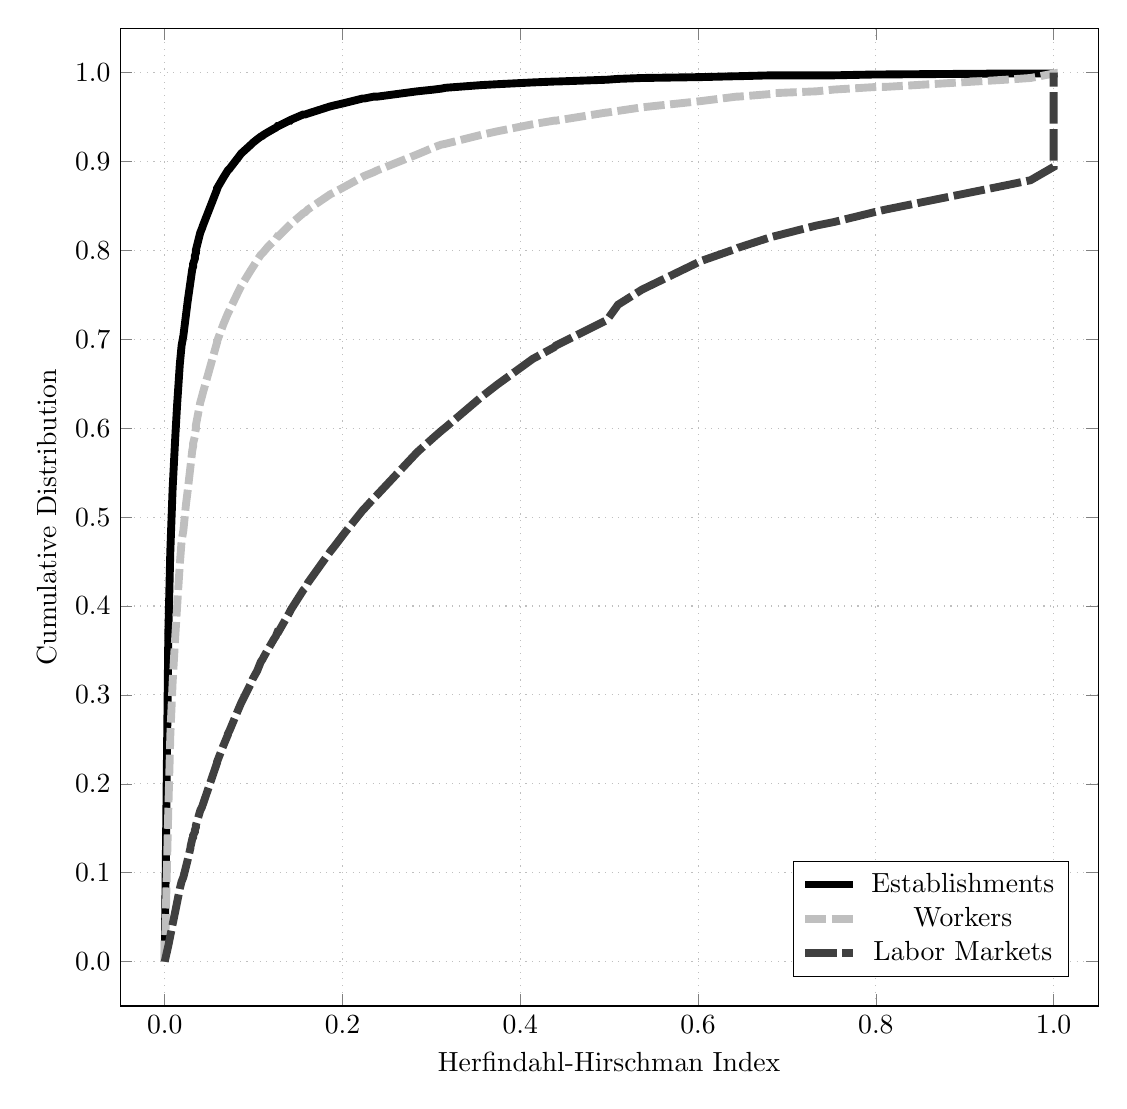
\begin{tikzpicture}
\begin{axis}[ytick={0,0.1,0.2,0.3,0.4,0.5,0.6,0.7,0.8,0.9,1}, height=14cm, width=14cm, grid=major, grid style = dotted, xtick={0,0.2,0.4,0.6,0.8,1}, xlabel=Herfindahl-Hirschman Index,ylabel=Cumulative Distribution, xmin=-0.05, xmax=1.05, ymin = -0.05, ymax=1.05, legend pos = south east, y tick label style={/pgf/number format/.cd,fixed,fixed zerofill, precision=1,/tikz/.cd},x tick label style={/pgf/number format/.cd,fixed,fixed zerofill, precision=1,/tikz/.cd}]

\addplot[mark=none, solid, color=black, line width=1mm] coordinates { (0,0)  (.0041,.37) (.0061,.453) (.0063,.461) (.0089,.532) (.012,.592) (.014,.627) (.015,.642) (.017,.672) (.019,.693) (.021,.704) (.024,.728) (.026,.744) (.029,.765) (.029,.765) (.031,.779) (.032,.782) (.032,.785) (.034,.791) (.034,.794) (.035,.797) (.035,.8) (.04,.82) (.042,.825) (.043,.828) (.059,.869) (.059,.87) (.066,.882) (.071,.89) (.071,.89) (.073,.892) (.083,.905) (.086,.909) (.086,.909) (.097,.919) (.099,.921) (.104,.925) (.108,.928) (.11,.929) (.111,.93) (.116,.933) (.123,.937) (.125,.938) (.127,.94) (.128,.94) (.14,.946) (.141,.946) (.141,.946) (.142,.947) (.156,.953) (.158,.953) (.161,.954) (.186,.962) (.19,.963) (.203,.966) (.203,.966) (.203,.966) (.223,.971) (.225,.971) (.235,.973) (.239,.973) (.284,.979) (.303,.981) (.311,.982) (.316,.983) (.356,.986) (.374,.987) (.414,.989) (.438,.99) (.44,.99) (.496,.992) (.497,.992) (.51,.993) (.537,.994) (.603,.995) (.643,.996) (.645,.996) (.682,.997) (.686,.997) (.733,.997) (.753,.997) (.802,.998) (.811,.998) (.945,.999) (.974,.999) (1,.999) (1,1) (1,.999) (1,.999) (1,.999) (1,.999) (1,1) (1,1) (1,.999) (1,.999) (1,.999) (1,1)};

\addplot[mark=none, dash pattern = on 7.6pt off 2pt, color=lightgray, line width=1mm] coordinates { (0,0)  (.0041,.173) (.0061,.245) (.0063,.254) (.0089,.314) (.012,.368) (.014,.4) (.015,.416) (.017,.447) (.019,.473) (.021,.485) (.024,.515) (.026,.531) (.029,.557) (.029,.557) (.031,.575) (.032,.58) (.032,.583) (.034,.591) (.034,.594) (.035,.599) (.035,.603) (.04,.629) (.042,.636) (.043,.64) (.059,.697) (.059,.698) (.066,.717) (.071,.729) (.071,.729) (.073,.733) (.083,.754) (.086,.76) (.086,.76) (.097,.778) (.099,.781) (.104,.789) (.108,.795) (.11,.797) (.111,.798) (.116,.804) (.123,.811) (.125,.813) (.127,.816) (.128,.816) (.14,.828) (.141,.829) (.141,.829) (.142,.83) (.156,.842) (.158,.843) (.161,.846) (.186,.863) (.19,.865) (.203,.872) (.203,.872) (.203,.872) (.223,.883) (.225,.884) (.235,.888) (.239,.89) (.284,.908) (.303,.916) (.311,.919) (.316,.92) (.356,.93) (.374,.934) (.414,.942) (.438,.946) (.44,.946) (.496,.955) (.497,.955) (.51,.957) (.537,.961) (.603,.968) (.643,.973) (.645,.973) (.682,.976) (.686,.977) (.733,.979) (.753,.981) (.802,.984) (.811,.984) (.945,.992) (.974,.994) (1,.999) (1,.998) (1,1) (1,.997) (1,.997) (1,.999) (1,.997) (1,.998) (1,.997) (1,.998) (1,.999) (1,1)};

\addplot[mark=none, dash pattern = on 11.4pt off 2pt, color=darkgray, line width=1mm] coordinates { (0,0)  (.0041,.018) (.0061,.028) (.0063,.029) (.0089,.042) (.012,.057) (.014,.067) (.015,.072) (.017,.082) (.019,.09) (.021,.095) (.024,.107) (.026,.115) (.029,.128) (.029,.129) (.031,.138) (.032,.14) (.032,.142) (.034,.146) (.034,.148) (.035,.151) (.035,.153) (.04,.17) (.042,.174) (.043,.177) (.059,.224) (.059,.225) (.066,.243) (.071,.255) (.071,.256) (.073,.26) (.083,.284) (.086,.291) (.086,.291) (.097,.313) (.099,.318) (.104,.327) (.108,.337) (.11,.34) (.111,.342) (.116,.351) (.123,.363) (.125,.366) (.127,.371) (.128,.371) (.14,.392) (.141,.394) (.141,.394) (.142,.396) (.156,.418) (.158,.42) (.161,.426) (.186,.461) (.19,.466) (.203,.483) (.203,.483) (.203,.483) (.223,.508) (.225,.51) (.235,.521) (.239,.525) (.284,.573) (.303,.59) (.311,.597) (.316,.601) (.356,.635) (.374,.649) (.414,.678) (.438,.691) (.44,.693) (.496,.721) (.497,.721) (.51,.739) (.537,.756) (.603,.788) (.643,.802) (.645,.803) (.682,.815) (.686,.816) (.733,.828) (.753,.832) (.802,.844) (.811,.846) (.945,.873) (.974,.879) (1,.894) (1,.896) (1,.912) (1,.936) (1,.94) (1,.956) (1,.966) (1,.967) (1,.983) (1,.988) (1,.989) (1,1)};

\legend{~Establishments,~Workers,~Labor Markets}
\end{axis}
\end{tikzpicture}
}
\floatfoot{ \footnotesize \textsc{Note. ---} The figure illustrates smoothed empirical cumulative distribution functions of labor market concentration in Germany for three different units of observation: establishments, workers, and labor markets. Labor market concentration refers to employment-based HHIs for combinations of NACE-4 industries and commuting zones and is tracked with annual frequency. The cumulative distribution functions of establishments and workers are generated on the basis of respective frequency weights. HHI = Herfindahl-Hirschman Index. NACE-4 = 4-Digit Statistical Nomenclature of Economic Activities in the European Community. Source: IEB, 1999-2017.}
\end{figure}




\vspace*{\fill}
\clearpage
\vspace*{\fill}

\begin{figure}[!ht]
\centering
\caption{Trend in Labor Market Concentration by Concentration Measure}
\label{fig:C3}
\scalebox{0.80}{
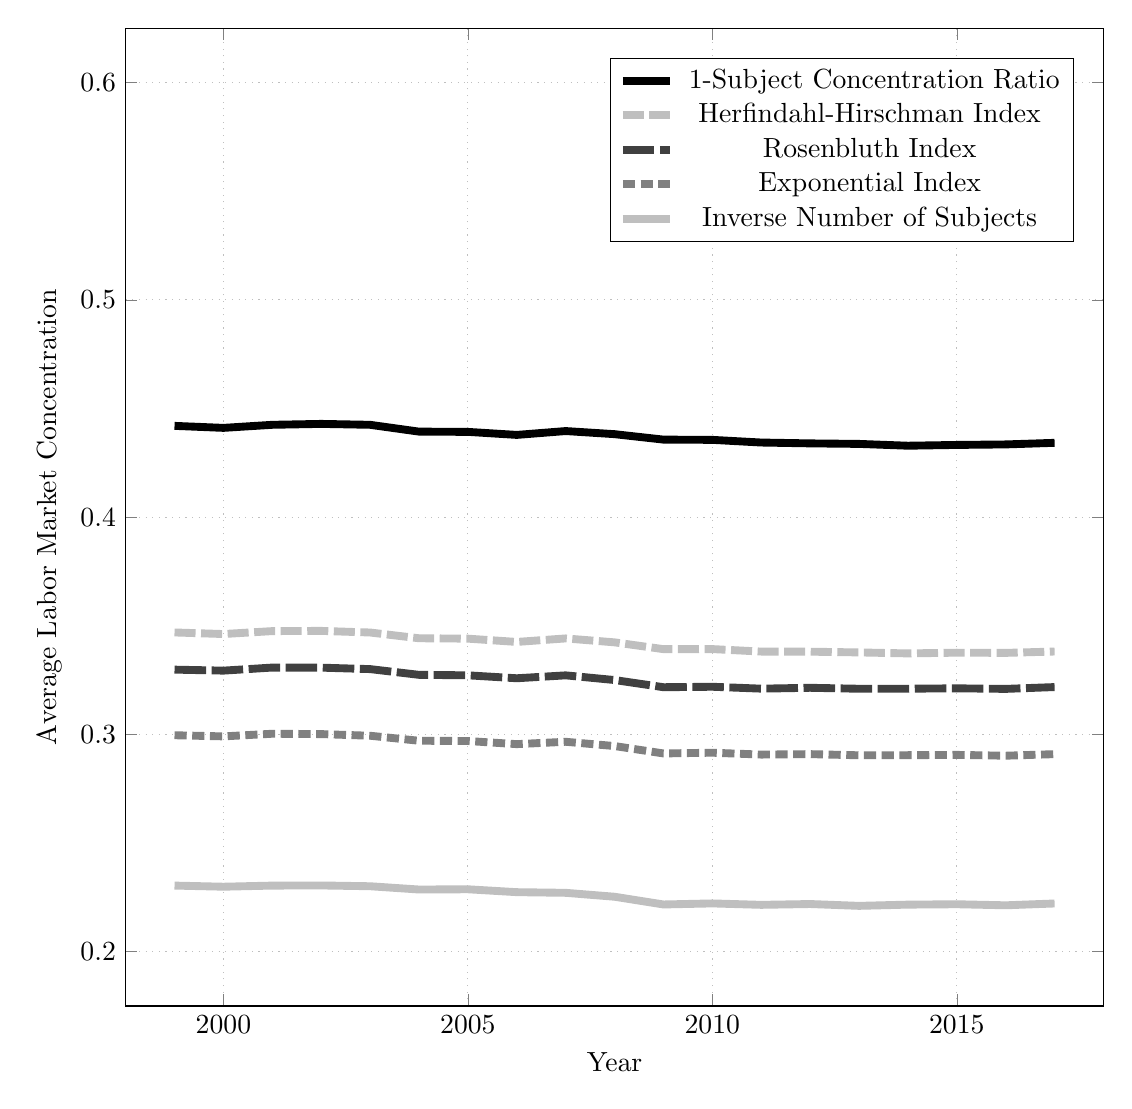
\begin{tikzpicture}
\begin{axis}[ytick={0.2,0.3,0.4,0.5,0.6}, height=14cm, width=14cm, grid=major, grid style = dotted, xtick={2000,2005,2010,2015}, xlabel=Year, ylabel=Average Labor Market Concentration, ymin=0.175, ymax=0.625, xmin=1998, xmax=2018, legend pos = north east, y tick label style={/pgf/number format/.cd,fixed,fixed zerofill, precision=1,/tikz/.cd}]

\addplot[mark=none, solid, color=black, line width=1mm] coordinates { (1999,.44199985) (2000,.44107428) (2001,.44248751) (2002,.44290555) (2003,.44248438) (2004,.4393515) (2005,.43923345) (2006,.43783769) (2007,.43961072) (2008,.43818289) (2009,.43567145) (2010,.43556038) (2011,.4343293) (2012,.43393832) (2013,.43369806) (2014,.43286532) (2015,.43322325) (2016,.43345851) (2017,.43419126) };

\addplot[mark=none, dash pattern = on 7.6pt off 2pt, color=lightgray, line width=1mm] coordinates { (1999,.34692895) (2000,.34619635) (2001,.34754792) (2002,.34764645) (2003,.34689844) (2004,.34425455) (2005,.34407568) (2006,.34256384) (2007,.34418085) (2008,.34237429) (2009,.3392415) (2010,.33927205) (2011,.3381308) (2012,.33807713) (2013,.33773673) (2014,.33728316) (2015,.33761665) (2016,.33752686) (2017,.33815241) };

\addplot[mark=none, dash pattern = on 11.4pt off 2pt, color=darkgray, line width=1mm] coordinates { (1999,.32981464) (2000,.32935843) (2001,.33077019) (2002,.33072925) (2003,.33005968) (2004,.32742405) (2005,.32720327) (2006,.32584572) (2007,.32718578) (2008,.32502899) (2009,.32172766) (2010,.32193482) (2011,.32106307) (2012,.32145905) (2013,.32101721) (2014,.3210429) (2015,.32121494) (2016,.32095286) (2017,.32179528) };

\addplot[mark=none, dash pattern = on 4.4pt off 2pt, color=gray, line width=1mm] coordinates { (1999,.29962295) (2000,.2990967) (2001,.30031231) (2002,.30015108) (2003,.2993955) (2004,.2970908) (2005,.29696983) (2006,.29552904) (2007,.29661399) (2008,.29464909) (2009,.29124704) (2010,.2915822) (2011,.29072464) (2012,.29092741) (2013,.29039735) (2014,.29044524) (2015,.29058278) (2016,.29020461) (2017,.29092625) };

\addplot[mark=none, solid, color=black!25!white, line width=1mm] coordinates { (1999,.23043729) (2000,.22991556) (2001,.23043101) (2002,.2304945) (2003,.23013274) (2004,.22862332) (2005,.22873777) (2006,.22740556) (2007,.22710556) (2008,.22530168) (2009,.22174202) (2010,.22222735) (2011,.22157301) (2012,.22194794) (2013,.22110565) (2014,.22167072) (2015,.22184791) (2016,.22136095) (2017,.22219706) };

\legend{~1-Subject Concentration Ratio, Herfindahl-Hirschman Index, Rosenbluth Index, Exponential Index, Inverse Number of Subjects}

\end{axis}
\end{tikzpicture}
}
\floatfoot{ \footnotesize \textsc{Note. ---} The figure reports means of selected concentration indices over time to visualize the development of labor market concentration in Germany. Labor market concentration refers to employment-based concentration indices for combinations of NACE-4 industries and commuting zones and is tracked with annual frequency. NACE-4 = 4-Digit Statistical Nomenclature of Economic Activities in the European Community. Source: IEB, 1999-2017.}
\end{figure}



\vspace*{\fill}

\end{landscape}
\clearpage


\begin{figure}[!ht]
\centering
\caption{Labor Market Concentration by NACE-4 Industry}
\label{fig:C4}
\scalebox{0.80}{
\includegraphics{A.pdf}
}
\floatfoot{ \scriptsize \textsc{Note. ---} The figure uses boxplots to visualize the distribution of labor market concentration by NACE-4 industries in Germany. Labor market concentration refers to employment-based HHIs for combinations of NACE-4 industries and commuting zones and is tracked with annual frequency. In each box, the center marks the median of the HHI distribution whereas left and right margins represent the 25th and 75th percentile. Lower and upper whiskers indicate the 5th and 95th percentile, respectively. Hollow squares illustrate the underlying means. Dots represent outliers (i.e., values below the 5th or above the 95th percentile). HHI = Herfindahl-Hirschman Index. NACE-4 = 4-Digit Statistical Nomenclature of Economic Activities in the European Community. Source: IEB, 1999-2017.}
\end{figure}
\begin{figure}[!ht]
\addtocounter{figure}{-1}
\centering
\caption{Labor Market Concentration by NACE-4 Industry (Cont.)}
%\label{fig:C4}
\scalebox{0.80}{
\includegraphics{B.pdf}
}
\floatfoot{ \scriptsize \textsc{Note. ---} The figure uses boxplots to visualize the distribution of labor market concentration by NACE-4 industries in Germany. Labor market concentration refers to employment-based HHIs for combinations of NACE-4 industries and commuting zones and is tracked with annual frequency. In each box, the center marks the median of the HHI distribution whereas left and right margins represent the 25th and 75th percentile. Lower and upper whiskers indicate the 5th and 95th percentile, respectively. Hollow squares illustrate the underlying means. Dots represent outliers (i.e., values below the 5th or above the 95th percentile). HHI = Herfindahl-Hirschman Index. NACE-4 = 4-Digit Statistical Nomenclature of Economic Activities in the European Community. Source: IEB, 1999-2017.}
\end{figure}
\begin{figure}[!ht]
\addtocounter{figure}{-1}
\centering
\caption{Labor Market Concentration by NACE-4 Industry (Cont.)}
%\label{fig:C4}
\scalebox{0.80}{
\includegraphics{C.pdf}
}
\floatfoot{ \scriptsize \textsc{Note. ---} The figure uses boxplots to visualize the distribution of labor market concentration by NACE-4 industries in Germany. Labor market concentration refers to employment-based HHIs for combinations of NACE-4 industries and commuting zones and is tracked with annual frequency. In each box, the center marks the median of the HHI distribution whereas left and right margins represent the 25th and 75th percentile. Lower and upper whiskers indicate the 5th and 95th percentile, respectively. Hollow squares illustrate the underlying means. Dots represent outliers (i.e., values below the 5th or above the 95th percentile). HHI = Herfindahl-Hirschman Index. NACE-4 = 4-Digit Statistical Nomenclature of Economic Activities in the European Community. Source: IEB, 1999-2017.}
\end{figure}
\begin{figure}[!ht]
\addtocounter{figure}{-1}
\centering
\caption{Labor Market Concentration by NACE-4 Industry (Cont.)}
%\label{fig:C4}
\scalebox{0.80}{
\includegraphics{D.pdf}
}
\floatfoot{ \scriptsize \textsc{Note. ---} The figure uses boxplots to visualize the distribution of labor market concentration by NACE-4 industries in Germany. Labor market concentration refers to employment-based HHIs for combinations of NACE-4 industries and commuting zones and is tracked with annual frequency. In each box, the center marks the median of the HHI distribution whereas left and right margins represent the 25th and 75th percentile. Lower and upper whiskers indicate the 5th and 95th percentile, respectively. Hollow squares illustrate the underlying means. Dots represent outliers (i.e., values below the 5th or above the 95th percentile). HHI = Herfindahl-Hirschman Index. NACE-4 = 4-Digit Statistical Nomenclature of Economic Activities in the European Community. Source: IEB, 1999-2017.}
\end{figure}
\begin{figure}[!ht]
\addtocounter{figure}{-1}
\centering
\caption{Labor Market Concentration by NACE-4 Industry (Cont.)}
%\label{fig:C4}
\scalebox{0.80}{
\includegraphics{E.pdf}
}
\floatfoot{ \scriptsize \textsc{Note. ---} The figure uses boxplots to visualize the distribution of labor market concentration by NACE-4 industries in Germany. Labor market concentration refers to employment-based HHIs for combinations of NACE-4 industries and commuting zones and is tracked with annual frequency. In each box, the center marks the median of the HHI distribution whereas left and right margins represent the 25th and 75th percentile. Lower and upper whiskers indicate the 5th and 95th percentile, respectively. Hollow squares illustrate the underlying means. Dots represent outliers (i.e., values below the 5th or above the 95th percentile). HHI = Herfindahl-Hirschman Index. NACE-4 = 4-Digit Statistical Nomenclature of Economic Activities in the European Community. Source: IEB, 1999-2017.}
\end{figure}
\begin{figure}[!ht]
\addtocounter{figure}{-1}
\centering
\caption{Labor Market Concentration by NACE-4 Industry (Cont.)}
%\label{fig:C4}
\scalebox{0.80}{
\includegraphics{F.pdf}
}
\floatfoot{ \scriptsize \textsc{Note. ---} The figure uses boxplots to visualize the distribution of labor market concentration by NACE-4 industries in Germany. Labor market concentration refers to employment-based HHIs for combinations of NACE-4 industries and commuting zones and is tracked with annual frequency. In each box, the center marks the median of the HHI distribution whereas left and right margins represent the 25th and 75th percentile. Lower and upper whiskers indicate the 5th and 95th percentile, respectively. Hollow squares illustrate the underlying means. Dots represent outliers (i.e., values below the 5th or above the 95th percentile). HHI = Herfindahl-Hirschman Index. NACE-4 = 4-Digit Statistical Nomenclature of Economic Activities in the European Community. Source: IEB, 1999-2017.}
\end{figure}
\begin{figure}[!ht]
\addtocounter{figure}{-1}
\centering
\caption{Labor Market Concentration by NACE-4 Industry (Cont.)}
%\label{fig:C4}
\scalebox{0.80}{
\includegraphics{G.pdf}
}
\floatfoot{ \scriptsize \textsc{Note. ---} The figure uses boxplots to visualize the distribution of labor market concentration by NACE-4 industries in Germany. Labor market concentration refers to employment-based HHIs for combinations of NACE-4 industries and commuting zones and is tracked with annual frequency. In each box, the center marks the median of the HHI distribution whereas left and right margins represent the 25th and 75th percentile. Lower and upper whiskers indicate the 5th and 95th percentile, respectively. Hollow squares illustrate the underlying means. Dots represent outliers (i.e., values below the 5th or above the 95th percentile). HHI = Herfindahl-Hirschman Index. NACE-4 = 4-Digit Statistical Nomenclature of Economic Activities in the European Community. Source: IEB, 1999-2017.}
\end{figure}
\begin{figure}[!ht]
\addtocounter{figure}{-1}
\centering
\caption{Labor Market Concentration by NACE-4 Industry (Cont.)}
%\label{fig:C4}
\scalebox{0.80}{
\includegraphics{H.pdf}
}
\floatfoot{ \scriptsize \textsc{Note. ---} The figure uses boxplots to visualize the distribution of labor market concentration by NACE-4 industries in Germany. Labor market concentration refers to employment-based HHIs for combinations of NACE-4 industries and commuting zones and is tracked with annual frequency. In each box, the center marks the median of the HHI distribution whereas left and right margins represent the 25th and 75th percentile. Lower and upper whiskers indicate the 5th and 95th percentile, respectively. Hollow squares illustrate the underlying means. Dots represent outliers (i.e., values below the 5th or above the 95th percentile). HHI = Herfindahl-Hirschman Index. NACE-4 = 4-Digit Statistical Nomenclature of Economic Activities in the European Community. Source: IEB, 1999-2017.}
\end{figure}
\begin{figure}[!ht]
\addtocounter{figure}{-1}
\centering
\caption{Labor Market Concentration by NACE-4 Industry (Cont.)}
%\label{fig:C4}
\scalebox{0.80}{
\includegraphics{I.pdf}
}
\floatfoot{ \scriptsize \textsc{Note. ---} The figure uses boxplots to visualize the distribution of labor market concentration by NACE-4 industries in Germany. Labor market concentration refers to employment-based HHIs for combinations of NACE-4 industries and commuting zones and is tracked with annual frequency. In each box, the center marks the median of the HHI distribution whereas left and right margins represent the 25th and 75th percentile. Lower and upper whiskers indicate the 5th and 95th percentile, respectively. Hollow squares illustrate the underlying means. Dots represent outliers (i.e., values below the 5th or above the 95th percentile). HHI = Herfindahl-Hirschman Index. NACE-4 = 4-Digit Statistical Nomenclature of Economic Activities in the European Community. Source: IEB, 1999-2017.}
\end{figure}

\clearpage
\vspace*{\fill}


\begin{figure}[!ht]
\centering
\caption{Labor Market Concentration by Commuting Zone}
\label{fig:C5}
\scalebox{0.80}{
\includegraphics{J.pdf}
}
\floatfoot{ \scriptsize \textsc{Note. ---} The figure uses boxplots to visualize the distribution of labor market concentration by commuting zones in Germany. Labor market concentration refers to employment-based HHIs for combinations of NACE-4 industries and commuting zones and is tracked with annual frequency. In each box, the center marks the median of the HHI distribution whereas left and right margins represent the 25th and 75th percentile. Lower and upper whiskers indicate the 5th and 95th percentile, respectively. Hollow squares illustrate the underlying means. Dots represent outliers (i.e., values below the 5th or above the 95th percentile). HHI = Herfindahl-Hirschman Index. NACE-4 = 4-Digit Statistical Nomenclature of Economic Activities in the European Community. Source: IEB, 1999-2017.}
\end{figure}


\vspace*{\fill}
\clearpage
\vspace*{\fill}

\begin{figure}[!ht]
\centering
\caption{Labor Market Concentration by NUTS-3 Regions}
\label{fig:C6}
\scalebox{1}{

\includegraphics[page=1,width=.95\textwidth]{Figure_C6.pdf}

}
\floatfoot{ \footnotesize \textsc{Note. ---} The map displays average labor market concentration by NUTS-3 regions in Germany. Labor market concentration refers to employment-based HHIs for combinations of NACE-4 industries and commuting zones and is tracked with annual frequency. HHI = Herfindahl-Hirschman Index. NACE-4 = 4-Digit Statistical Nomenclature of Economic Activities in the European Community. NUTS-3 = 3-Digit Statistical Nomenclature of Territorial Units in the European Community. Source: IEB, 1999-2017.}
\end{figure}



\vspace*{\fill}
%\clearpage



\begin{landscape}



\section{Appendix: Effects of Labor Market Concentration}
\label{sec:D}
\setcounter{table}{0} % reset table counter
\setcounter{figure}{0} % reset figure counter

\vspace*{0.6cm}




\begin{table}[!ht]
\centering
%\resizebox{\textwidth}{!}{
\scalebox{0.90}{
\begin{threeparttable}
\caption{Effects of LM Concentration on Earnings by Labor Market Definition}
\label{tab:D1}
\begin{tabular}{|C{4cm}|C{2.7cm}C{2.7cm}C{2.7cm}C{2.7cm}|} \hline \hline
\multirow{4}{*}{\diagbox[height=4.4175\line, innerwidth=4cm]{Regressor}{\shortstack{ \\ \hspace{0.1cm}Dependent \\ \hspace{0.1cm}Variable }}} & \multirow{4.4}{*}{\shortstack{(1) \\ Log \\ Mean Daily\vphantom{/} \\ Wages }} & \multirow{4.4}{*}{\shortstack{(2) \\ Log \\ Mean Daily\vphantom{/} \\ Wages }} & \multirow{4.4}{*}{\shortstack{(3) \\ Log \\ Mean Daily\vphantom{/} \\ Wages }} & \multirow{4.4}{*}{\shortstack{(4) \\ Log \\ Mean Daily\vphantom{/} \\ Wages }} \\
&&&& \\
&&&& \\
&&&& \\[0.2cm] \hline
\multirow{2.4}{*}{Log HHI} &  \multirow{2.4}{*}{\shortstack{\hphantom{***}-0.060***\hphantom{-}  \\ (0.008)}}  & \multirow{2.4}{*}{\shortstack{\hphantom{***}-0.052***\hphantom{-}  \\ (0.005)}} & \multirow{2.4}{*}{\shortstack{\hphantom{***}-0.068***\hphantom{-}  \\ (0.004)}} & \multirow{2.4}{*}{\shortstack{\hphantom{***}-0.043***\hphantom{-}  \\ (0.006)}}   \\
&&&& \\[0.2cm] \hdashline
&&&& \\[-0.2cm]
Instrument  & $ \overline{\text{Log}\,\,\text{INS}} \,\,\backslash\, \{c\} $ & $ \overline{\text{Log}\,\,\text{INS}} \,\,\backslash\, \{c\} $ & $ \overline{\text{Log}\,\,\text{INS}} \,\,\backslash\, \{c\} $ & $ \overline{\text{Log}\,\,\text{INS}} \,\,\backslash\, \{c\} $  \\
\multirow{2.4}{*}{\shortstack{Fixed \\ Effects}}  & \multirow{2.4}{*}{\shortstack{Establishment \\ Year $\times$ CZ}} &  \multirow{2.4}{*}{\shortstack{Establishment \\ Year $\times$ CZ}} & \multirow{2.4}{*}{\shortstack{Establishment \\ Year $\times$ NUTS-3}} &  \multirow{2.4}{*}{\shortstack{Establishment \\ Year $\times$ CZ}} \\
&&&& \\
\multirow{3.4}{*}{\shortstack{Labor Market \\ Definition \\ (Object)}}  & \multirow{3.4}{*}{\shortstack{NACE-3 \\ $\times$ CZ \\ (Employment)}} & \multirow{3.4}{*}{\shortstack{NACE-5 \\ $\times$ CZ \\ (Employment)}} & \multirow{3.4}{*}{\shortstack{NACE-4 \\ $\times$ NUTS-3 \\ (Employment)}} & \multirow{3.4}{*}{\shortstack{NACE-4 \\ $\times$ CZ \\ (Hires)}} \\
&&&&  \\
&&&&  \\[0.2cm] \hdashline
&&&&  \\[-0.4cm]
\multirow{2.4}{*}{Sample}  & \multirow{2.4}{*}{1999-2014} & \multirow{2.4}{*}{1999-2014}  & \multirow{2.4}{*}{1999-2014}  & \multirow{2.4}{*}{2000-2014}  \\
&&&& \\[0.2cm] \hdashline
&&&& \\[-0.2cm]
Observations &  2,139,426       & 2,139,426       & 2,139,426       & 1,958,623         \\[0.2cm]
F Statistic & 253.3 & 565.8 & 2561.3 & 548.3 \\[0.2cm]  \hline \hline
\end{tabular}
\begin{tablenotes}
\item \footnotesize \textsc{Note. ---} The table displays fixed effects regressions of log establishment-level means of daily wages (of regular full-time workers) on the log of HHI. The instrumental variable refers to the leave-one-out industry average of the log inverse number of firms across commuting zones. Standard errors (in parentheses) are clustered at the labor-market level. CZ = Commuting Zone. HHI = Herfindahl-Hirschman Index. INS = Inverse Number of Subjects. LM = Labor Market. NACE-4 = 4-Digit Statistical Nomenclature of Economic Activities in the European Community. NUTS-X = X-Digit Statistical Nomenclature of Territorial Units. * = p$<$0.10. ** = p$<$0.05. *** = p$<$0.01. Sources: IEB $\plus$ BHP, 1999-2014.
\end{tablenotes}
\end{threeparttable}
}
\end{table}


\vspace*{\fill}
\clearpage
\vspace*{\fill}


\begin{table}[!ht]
\centering
%\resizebox{\textwidth}{!}{
\scalebox{0.90}{
\begin{threeparttable}
\caption{Effects of LM Concentration on Earnings by Concentration Measure}
\label{tab:D2}
\begin{tabular}{|C{4cm}|C{2.7cm}C{2.7cm}C{2.7cm}C{2.7cm}|} \hline \hline
\multirow{4}{*}{\diagbox[height=4.4175\line, innerwidth=4cm]{Regressor}{\shortstack{ \\ \hspace{0.1cm}Dependent \\ \hspace{0.1cm}Variable }}} & \multirow{4.4}{*}{\shortstack{(1) \\ Log \\ Mean Daily\vphantom{/} \\ Wages }} & \multirow{4.4}{*}{\shortstack{(2) \\ Log \\ Mean Daily\vphantom{/} \\ Wages }} & \multirow{4.4}{*}{\shortstack{(3) \\ Log \\ Mean Daily\vphantom{/} \\ Wages }} & \multirow{4.4}{*}{\shortstack{(4) \\ Log \\ Mean Daily\vphantom{/} \\ Wages }} \\
&&&& \\
&&&& \\
&&&& \\[0.2cm] \hline
\multirow{2.4}{*}{Log RBI}  & \multirow{2.4}{*}{\shortstack{\hphantom{***}-0.041***\hphantom{-} \\ (0.005)}}   &   &   & \\
&&&&  \\
\multirow{2.4}{*}{Log CR1}  &      & \multirow{2.4}{*}{\shortstack{\hphantom{***}-0.065***\hphantom{-} \\ (0.009)}}       &    &  \\
&&&&  \\
\multirow{2.4}{*}{Log INS}  &      &       & \multirow{2.4}{*}{\shortstack{\hphantom{***}-0.040***\hphantom{-} \\ (0.004)}}   &  \\
&&&&  \\
\multirow{2.4}{*}{Log EXP}  &      &       &       &  \multirow{2.4}{*}{\shortstack{\hphantom{***}-0.041***\hphantom{-} \\ (0.005)}} \\
&&&&  \\[0.2cm] \hdashline
&&&& \\[-0.2cm]
Instrument  & $ \overline{\text{Log}\,\,\text{INS}} \,\,\backslash\, \{c\} $ & $ \overline{\text{Log}\,\,\text{INS}} \,\,\backslash\, \{c\} $ & $ \overline{\text{Log}\,\,\text{INS}} \,\,\backslash\, \{c\} $ & $ \overline{\text{Log}\,\,\text{INS}} \,\,\backslash\, \{c\} $  \\
\multirow{2.4}{*}{\shortstack{Fixed \\ Effects}}  & \multirow{2.4}{*}{\shortstack{Establishment \\ Year $\times$ CZ}} &  \multirow{2.4}{*}{\shortstack{Establishment \\ Year $\times$ CZ}} & \multirow{2.4}{*}{\shortstack{Establishment \\ Year $\times$ CZ}} &  \multirow{2.4}{*}{\shortstack{Establishment \\ Year $\times$ CZ}} \\
&&&& \\
\multirow{3.4}{*}{\shortstack{Labor Market \\ Definition \\ (Object)}}  & \multirow{3.4}{*}{\shortstack{NACE-4 \\ $\times$ CZ \\ (Employment)}} & \multirow{3.4}{*}{\shortstack{NACE-4 \\ $\times$ CZ \\ (Employment)}} & \multirow{3.4}{*}{\shortstack{NACE-4 \\ $\times$ CZ \\ (Employment)}} & \multirow{3.4}{*}{\shortstack{NACE-4 \\ $\times$ CZ \\ (Employment)}} \\
&&&& \\
&&&& \\[0.2cm] \hdashline
&&&& \\[-0.2cm]
Observations &  2,139,426       & 2,139,426       & 2,139,426       & 2,139,426         \\[0.2cm]
F Statistic & 3422.3 & 157.1 & 5555.7 & 2107.1 \\[0.2cm]  \hline \hline
\end{tabular}
\begin{tablenotes}
\item \footnotesize \textsc{Note. ---} The table displays fixed effects regressions of log establishment-level means of daily wages (of regular full-time workers) on the log of the concentration index. The instrumental variable refers to the leave-one-out industry average of the log inverse number of firms across commuting zones. Standard errors (in parentheses) are clustered at the labor-market level. CR1 = 1-Subject Concentration Ratio. CZ = Commuting Zone. EXP = Exponential Index. HHI = Herfindahl-Hirschman Index. INS = Inverse Number of Subjects. LM = Labor Market. NACE-4 = 4-Digit Statistical Nomenclature of Economic Activities in the European Community. RBI = Rosenbluth Index. * = p$<$0.10. ** = p$<$0.05. *** = p$<$0.01. Sources: IEB $\plus$ BHP, 1999-2014.
\end{tablenotes}
\end{threeparttable}
}
\end{table}




\vspace*{\fill}
\clearpage
\vspace*{\fill}



\begin{table}[!ht]
\centering
%\resizebox{\textwidth}{!}{
\scalebox{0.90}{
\begin{threeparttable}
\caption{Effects of LM Concentration on Earnings by Territory}
\label{tab:D3}
\begin{tabular}{|C{4cm}|C{5.8cm}C{5.8cm}|} \hline \hline
\multirow{4}{*}{\diagbox[height=4.4175\line, innerwidth=4cm]{Regressor}{\shortstack{ \\ \hspace{0.1cm}Dependent \\ \hspace{0.1cm}Variable }}} & \multirow{4.4}{*}{\shortstack{(1) \\ Log \\ Mean Daily\vphantom{/} \\ Wages }} & \multirow{4.4}{*}{\shortstack{(2) \\ Log \\ Mean Daily\vphantom{/} \\ Wages }}  \\
&& \\
&& \\
&& \\[0.2cm] \hline
\multirow{2.4}{*}{Log HHI} &  \multirow{2.4}{*}{\shortstack{\hphantom{***}-0.047***\hphantom{-}  \\ (0.007)}}  & \multirow{2.4}{*}{\shortstack{\hphantom{***}-0.041***\hphantom{-}  \\ (0.009)}}   \\
&& \\[0.2cm] \hdashline
&& \\[-0.2cm]
Instrument  & $ \overline{\text{Log}\,\,\text{INS}} \,\,\backslash\, \{c\} $ & $ \overline{\text{Log}\,\,\text{INS}} \,\,\backslash\, \{c\} $   \\
\multirow{2.4}{*}{\shortstack{Fixed \\ Effects}}  & \multirow{2.4}{*}{\shortstack{Establishment \\ Year $\times$ CZ}} &  \multirow{2.4}{*}{\shortstack{Establishment \\ Year $\times$ CZ}}  \\
&& \\
\multirow{3.4}{*}{\shortstack{Labor Market \\ Definition \\ (Object)}}  & \multirow{3.4}{*}{\shortstack{NACE-4 \\ $\times$ CZ \\ (Employment)}} & \multirow{3.4}{*}{\shortstack{NACE-4 \\ $\times$ CZ \\ (Employment)}}  \\
&& \\
&& \\[0.2cm] \hdashline
&& \\[-0.4cm]
\multirow{2.4}{*}{Sample}  & \multirow{2.4}{*}{West Germany} & \multirow{2.4}{*}{\shortstack{East Germany \\ Berlin}}  \\
&& \\[0.2cm] \hdashline
&& \\[-0.2cm]
Observations &  1,676,484       & 462,942               \\[0.2cm]
F Statistic & 311.7 & 330.4   \\[0.2cm]  \hline \hline
\end{tabular}
\begin{tablenotes}
\item \footnotesize \textsc{Note. ---} The table displays fixed effects regressions of log establishment-level means of daily wages (of regular full-time workers) on the log of HHI. The instrumental variable refers to the leave-one-out industry average of the log inverse number of firms across commuting zones. Standard errors (in parentheses) are clustered at the labor-market level. CZ = Commuting Zone. HHI = Herfindahl-Hirschman Index. INS = Inverse Number of Subjects. LM = Labor Market. NACE-4 = 4-Digit Statistical Nomenclature of Economic Activities in the European Community. * = p$<$0.10. ** = p$<$0.05. *** = p$<$0.01. Sources: IEB $\plus$ BHP, 1999-2014.
\end{tablenotes}
\end{threeparttable}
}
\end{table}



\vspace*{\fill}
\clearpage
\vspace*{\fill}


\begin{table}[!ht]
\centering
%\resizebox{\textwidth}{!}{
\scalebox{0.90}{
\begin{threeparttable}
\caption{Effects of LM Concentration on Earnings by Percentile}
\label{tab:D4}
\begin{tabular}{|C{4cm}|C{3.75cm}C{3.75cm}C{3.75cm}|} \hline \hline
\multirow{4}{*}{\diagbox[height=4.4175\line, innerwidth=4cm]{Regressor}{\shortstack{ \\ \hspace{0.1cm}Dependent \\ \hspace{0.1cm}Variable }}} & \multirow{4.4}{*}{\shortstack{(1) \\ Log \\ P25 Daily\vphantom{/} \\ Wages }} & \multirow{4.4}{*}{\shortstack{(2) \\ Log \\ P50 Daily\vphantom{/} \\ Wages }} & \multirow{4.4}{*}{\shortstack{(3) \\ Log \\ P75 Daily\vphantom{/} \\ Wages }}  \\
&&& \\
&&& \\
&&& \\[0.2cm] \hline
\multirow{2.4}{*}{Log HHI} &  \multirow{2.4}{*}{\shortstack{\hphantom{***}-0.024***\hphantom{-}  \\ (0.005)}}  & \multirow{2.4}{*}{\shortstack{\hphantom{***}-0.042***\hphantom{-}  \\ (0.006)}} & \multirow{2.4}{*}{\shortstack{\hphantom{***}-0.059***\hphantom{-}  \\ (0.007)}}   \\
&&& \\[0.2cm] \hdashline
&&& \\[-0.2cm]
Instrument  & $ \overline{\text{Log}\,\,\text{INS}} \,\,\backslash\, \{c\} $ & $ \overline{\text{Log}\,\,\text{INS}} \,\,\backslash\, \{c\} $ & $ \overline{\text{Log}\,\,\text{INS}} \,\,\backslash\, \{c\} $   \\
\multirow{2.4}{*}{\shortstack{Fixed \\ Effects}}  & \multirow{2.4}{*}{\shortstack{Establishment \\ Year $\times$ CZ}} &  \multirow{2.4}{*}{\shortstack{Establishment \\ Year $\times$ CZ}} & \multirow{2.4}{*}{\shortstack{Establishment \\ Year $\times$ CZ}}  \\
&&& \\
\multirow{3.4}{*}{\shortstack{Labor Market \\ Definition \\ (Object)}}  & \multirow{3.4}{*}{\shortstack{NACE-4 \\ $\times$ CZ \\ (Employment)}} & \multirow{3.4}{*}{\shortstack{NACE-4 \\ $\times$ CZ \\ (Employment)}} & \multirow{3.4}{*}{\shortstack{NACE-4 \\ $\times$ CZ \\ (Employment)}}  \\
&&& \\
&&& \\[0.2cm] \hdashline
&&& \\[-0.2cm]
Observations &  2,139,426       & 2,139,426       & 2,139,426           \\[0.2cm]
F Statistic & 430.8 & 430.8 & 430.8  \\[0.2cm]  \hline \hline
\end{tabular}
\begin{tablenotes}
\item \footnotesize \textsc{Note. ---} The table displays fixed effects regressions of log establishment-level percentiles of daily wages (of regular full-time workers) on the log of HHI. The instrumental variable refers to the leave-one-out industry average of the log inverse number of firms across commuting zones. Standard errors (in parentheses) are clustered at the labor-market level. CZ = Commuting Zone. HHI = Herfindahl-Hirschman Index. INS = Inverse Number of Subjects. LM = Labor Market. NACE-4 = 4-Digit Statistical Nomenclature of Economic Activities in the European Community. PX = Xth Percentile. * = p$<$0.10. ** = p$<$0.05. *** = p$<$0.01. Sources: IEB $\plus$ BHP, 1999-2014.
\end{tablenotes}
\end{threeparttable}
}
\end{table}


\vspace*{\fill}
\clearpage
\vspace*{\fill}


\begin{table}[!ht]
\centering
%\resizebox{\textwidth}{!}{
\scalebox{0.90}{
\begin{threeparttable}
\caption{Effects of LM Concentration on Earnings by Outward Mobility}
\label{tab:D5}
\begin{tabular}{|C{4cm}|C{3.75cm}C{3.75cm}C{3.75cm}|} \hline \hline
\multirow{4}{*}{\diagbox[height=4.4175\line, innerwidth=4cm]{Regressor}{\shortstack{ \\ \hspace{0.1cm}Dependent \\ \hspace{0.1cm}Variable }}} & \multirow{4.4}{*}{\shortstack{(1) \\ Log \\ Mean Daily\vphantom{/} \\ Wages }} & \multirow{4.4}{*}{\shortstack{(2) \\ Log \\ Mean Daily\vphantom{/} \\ Wages }} & \multirow{4.4}{*}{\shortstack{(3) \\ Log \\ Mean Daily\vphantom{/} \\ Wages }}  \\
&&& \\
&&& \\
&&& \\[0.2cm] \hline
\multirow{2.4}{*}{Log HHI} &  \multirow{2.4}{*}{\shortstack{\hphantom{***}-0.072***\hphantom{-}  \\ (0.014)}}  & \multirow{2.4}{*}{\shortstack{\hphantom{***}-0.043***\hphantom{-}  \\ (0.009)}} & \multirow{2.4}{*}{\shortstack{\hphantom{***}-0.038***\hphantom{-}  \\ (0.005)}}   \\
&&& \\[0.2cm] \hdashline
&&& \\[-0.2cm]
Instrument  & $ \overline{\text{Log}\,\,\text{INS}} \,\,\backslash\, \{c\} $ & $ \overline{\text{Log}\,\,\text{INS}} \,\,\backslash\, \{c\} $ & $ \overline{\text{Log}\,\,\text{INS}} \,\,\backslash\, \{c\} $   \\
\multirow{2.4}{*}{\shortstack{Fixed \\ Effects}}  & \multirow{2.4}{*}{\shortstack{Establishment \\ Year $\times$ CZ}} &  \multirow{2.4}{*}{\shortstack{Establishment \\ Year $\times$ CZ}} & \multirow{2.4}{*}{\shortstack{Establishment \\ Year $\times$ CZ}}  \\
&&& \\
\multirow{3.4}{*}{\shortstack{Labor Market \\ Definition \\ (Object)}}  & \multirow{3.4}{*}{\shortstack{NACE-4 \\ $\times$ CZ \\ (Employment)}} & \multirow{3.4}{*}{\shortstack{NACE-4 \\ $\times$ CZ \\ (Employment)}} & \multirow{3.4}{*}{\shortstack{NACE-4 \\ $\times$ CZ \\ (Employment)}}  \\
&&& \\
&&& \\[0.2cm] \hdashline
&&& \\[-0.4cm]
\multirow{2.4}{*}{Sample}  & \multirow{2.4}{*}{\shortstack{Low \vphantom{/} \\ Mobility}} & \multirow{2.4}{*}{\shortstack{Medium \vphantom{/} \\ Mobility}} & \multirow{2.4}{*}{\shortstack{High \vphantom{/} \\ Mobility}}  \\
&&& \\[0.2cm] \hdashline
&&& \\[-0.2cm]
Observations &  694,171         & 724,661         & 720,360             \\[0.2cm]
F Statistic & 204.8 & 217.3 & 713.8  \\[0.2cm]  \hline \hline
\end{tabular}
\begin{tablenotes}
\item \footnotesize \textsc{Note. ---} The table displays fixed effects regressions of log establishment-level means of daily wages (of regular full-time workers) on the log of HHI. The instrumental variable refers to the leave-one-out industry average of the log inverse number of firms across commuting zones. Outward Mobility is measured as the share of workers who take up a new job in another labor market when leaving the job at their previous establishment. Standard errors (in parentheses) are clustered at the labor-market level. CZ = Commuting Zone. HHI = Herfindahl-Hirschman Index. INS = Inverse Number of Subjects. LM = Labor Market. NACE-4 = 4-Digit Statistical Nomenclature of Economic Activities in the European Community. * = p$<$0.10. ** = p$<$0.05. *** = p$<$0.01. Sources: IEB $\plus$ BHP, 1999-2014.
\end{tablenotes}
\end{threeparttable}
}
\end{table}



\vspace*{\fill}
\clearpage
\vspace*{\fill}



\begin{table}[!ht]
\centering
%\resizebox{\textwidth}{!}{
\scalebox{0.90}{
\begin{threeparttable}
\caption{Effects of LM Concentration on Employment by Labor Market Definition}
\label{tab:D6}
\begin{tabular}{|C{4cm}|C{2.7cm}C{2.7cm}C{2.7cm}C{2.7cm}|} \hline \hline
\multirow{4}{*}{\diagbox[height=4.4175\line, innerwidth=4cm]{Regressor}{\shortstack{ \\ \hspace{0.1cm}Dependent \\ \hspace{0.1cm}Variable }}} & \multirow{4.4}{*}{\shortstack{(1) \\ Log \\ Regular FT\vphantom{/} \\ Employment }} & \multirow{4.4}{*}{\shortstack{(2) \\ Log \\ Regular FT\vphantom{/} \\ Employment }} & \multirow{4.4}{*}{\shortstack{(3) \\ Log \\ Regular FT\vphantom{/} \\ Employment }} & \multirow{4.4}{*}{\shortstack{(4) \\ Log \\ Regular FT\vphantom{/} \\ Employment }} \\
&&&& \\
&&&& \\
&&&& \\[0.2cm] \hline
\multirow{2.4}{*}{Log HHI} &  \multirow{2.4}{*}{\shortstack{\hphantom{***}-0.234***\hphantom{-}  \\ (0.027)}}  & \multirow{2.4}{*}{\shortstack{\hphantom{***}-0.156***\hphantom{-}  \\ (0.017)}} & \multirow{2.4}{*}{\shortstack{\hphantom{***}-0.232***\hphantom{-}  \\ (0.011)}} & \multirow{2.4}{*}{\shortstack{\hphantom{***}-0.172***\hphantom{-}  \\ (0.018)}}   \\
&&&& \\[0.2cm] \hdashline
&&&& \\[-0.2cm]
Instrument  & $ \overline{\text{Log}\,\,\text{INS}} \,\,\backslash\, \{c\} $ & $ \overline{\text{Log}\,\,\text{INS}} \,\,\backslash\, \{c\} $ & $ \overline{\text{Log}\,\,\text{INS}} \,\,\backslash\, \{c\} $ & $ \overline{\text{Log}\,\,\text{INS}} \,\,\backslash\, \{c\} $  \\
\multirow{2.4}{*}{\shortstack{Fixed \\ Effects}}  & \multirow{2.4}{*}{\shortstack{Establishment \\ Year $\times$ CZ}} &  \multirow{2.4}{*}{\shortstack{Establishment \\ Year $\times$ CZ}} & \multirow{2.4}{*}{\shortstack{Establishment \\ Year $\times$ NUTS-3}} &  \multirow{2.4}{*}{\shortstack{Establishment \\ Year $\times$ CZ}} \\
&&&& \\
\multirow{3.4}{*}{\shortstack{Labor Market \\ Definition \\ (Object)}}  & \multirow{3.4}{*}{\shortstack{NACE-3 \\ $\times$ CZ \\ (Employment)}} & \multirow{3.4}{*}{\shortstack{NACE-5 \\ $\times$ CZ \\ (Employment)}} & \multirow{3.4}{*}{\shortstack{NACE-4 \\ $\times$ NUTS-3 \\ (Employment)}} & \multirow{3.4}{*}{\shortstack{NACE-4 \\ $\times$ CZ \\ (Hires)}} \\
&&&&  \\
&&&&  \\[0.2cm] \hdashline
&&&&  \\[-0.4cm]
\multirow{2.4}{*}{Sample}  & \multirow{2.4}{*}{1999-2014} & \multirow{2.4}{*}{1999-2014}  & \multirow{2.4}{*}{1999-2014}  & \multirow{2.4}{*}{2000-2014}  \\
&&&& \\[0.2cm] \hdashline
&&&& \\[-0.2cm]
Observations &  2,139,426       & 2,139,426       & 2,139,426       & 1,958,623         \\[0.2cm]
F Statistic & 253.3 & 565.8 & 2561.3 & 548.3 \\[0.2cm]  \hline \hline
\end{tabular}
\begin{tablenotes}
\item \footnotesize \textsc{Note. ---} The table displays fixed effects regressions of log establishment-level employment (of regular full-time workers) on the log of HHI. The instrumental variable refers to the leave-one-out industry average of the log inverse number of firms across commuting zones. Standard errors (in parentheses) are clustered at the labor-market level. CZ = Commuting Zone. FT = Full-Time. HHI = Herfindahl-Hirschman Index. INS = Inverse Number of Subjects. LM = Labor Market. NACE-4 = 4-Digit Statistical Nomenclature of Economic Activities in the European Community. NUTS-X = X-Digit Statistical Nomenclature of Territorial Units. * = p$<$0.10. ** = p$<$0.05. *** = p$<$0.01. Sources: IEB $\plus$ BHP, 1999-2014.
\end{tablenotes}
\end{threeparttable}
}
\end{table}



\vspace*{\fill}
\clearpage
\vspace*{\fill}



\begin{table}[!ht]
\centering
%\resizebox{\textwidth}{!}{
\scalebox{0.90}{
\begin{threeparttable}
\caption{Effects of LM Concentration on Employment by Concentration Measure}
\label{tab:D7}
\begin{tabular}{|C{4cm}|C{2.7cm}C{2.7cm}C{2.7cm}C{2.7cm}|} \hline \hline
\multirow{4}{*}{\diagbox[height=4.4175\line, innerwidth=4cm]{Regressor}{\shortstack{ \\ \hspace{0.1cm}Dependent \\ \hspace{0.1cm}Variable }}} & \multirow{4.4}{*}{\shortstack{(1) \\ Log \\ Regular FT\vphantom{/} \\ Employment }} & \multirow{4.4}{*}{\shortstack{(2) \\ Log \\ Regular FT\vphantom{/} \\ Employment }} & \multirow{4.4}{*}{\shortstack{(3) \\ Log \\ Regular FT\vphantom{/} \\ Employment }} & \multirow{4.4}{*}{\shortstack{(4) \\ Log \\ Regular FT\vphantom{/} \\ Employment }} \\
&&&& \\
&&&& \\
&&&& \\[0.2cm] \hline
\multirow{2.4}{*}{Log RBI}  & \multirow{2.4}{*}{\shortstack{\hphantom{***}-0.139***\hphantom{-} \\ (0.014)}}   &   &   & \\
&&&&  \\
\multirow{2.4}{*}{Log CR1}  &      & \multirow{2.4}{*}{\shortstack{\hphantom{***}-0.222***\hphantom{-} \\ (0.031)}}       &    &  \\
&&&&  \\
\multirow{2.4}{*}{Log INS}  &      &       & \multirow{2.4}{*}{\shortstack{\hphantom{***}-0.135***\hphantom{-} \\ (0.014)}}   &  \\
&&&&  \\
\multirow{2.4}{*}{Log EXP}  &      &       &       &  \multirow{2.4}{*}{\shortstack{\hphantom{***}-0.141***\hphantom{-} \\ (0.015)}} \\
&&&&  \\[0.2cm] \hdashline
&&&& \\[-0.2cm]
Instrument  & $ \overline{\text{Log}\,\,\text{INS}} \,\,\backslash\, \{c\} $ & $ \overline{\text{Log}\,\,\text{INS}} \,\,\backslash\, \{c\} $ & $ \overline{\text{Log}\,\,\text{INS}} \,\,\backslash\, \{c\} $ & $ \overline{\text{Log}\,\,\text{INS}} \,\,\backslash\, \{c\} $  \\
\multirow{2.4}{*}{\shortstack{Fixed \\ Effects}}  & \multirow{2.4}{*}{\shortstack{Establishment \\ Year $\times$ CZ}} &  \multirow{2.4}{*}{\shortstack{Establishment \\ Year $\times$ CZ}} & \multirow{2.4}{*}{\shortstack{Establishment \\ Year $\times$ CZ}} &  \multirow{2.4}{*}{\shortstack{Establishment \\ Year $\times$ CZ}} \\
&&&& \\
\multirow{3.4}{*}{\shortstack{Labor Market \\ Definition \\ (Object)}}  & \multirow{3.4}{*}{\shortstack{NACE-4 \\ $\times$ CZ \\ (Employment)}} & \multirow{3.4}{*}{\shortstack{NACE-4 \\ $\times$ CZ \\ (Employment)}} & \multirow{3.4}{*}{\shortstack{NACE-4 \\ $\times$ CZ \\ (Employment)}} & \multirow{3.4}{*}{\shortstack{NACE-4 \\ $\times$ CZ \\ (Employment)}} \\
&&&& \\
&&&& \\[0.2cm] \hdashline
&&&& \\[-0.2cm]
Observations &  2,139,426       & 2,139,426       & 2,139,426       & 2,139,426         \\[0.2cm]
F Statistic & 3422.3 & 157.1 & 5555.7 & 2107.1 \\[0.2cm]  \hline \hline
\end{tabular}
\begin{tablenotes}
\item \footnotesize \textsc{Note. ---} The table displays fixed effects regressions of log establishment-level employment (of regular full-time workers) on the log of the concentration index. The instrumental variable refers to the leave-one-out industry average of the log inverse number of firms across commuting zones. Standard errors (in parentheses) are clustered at the labor-market level. CR1 = 1-Subject Concentration Ratio. CZ = Commuting Zone. EXP = Exponential Index. FT = Full-Time. HHI = Herfindahl-Hirschman Index. INS = Inverse Number of Subjects. LM = Labor Market. NACE-4 = 4-Digit Statistical Nomenclature of Economic Activities in the European Community. RBI = Rosenbluth Index. * = p$<$0.10. ** = p$<$0.05. *** = p$<$0.01. Sources: IEB $\plus$ BHP, 1999-2014.
\end{tablenotes}
\end{threeparttable}
}
\end{table}



\vspace*{\fill}
\clearpage
\vspace*{\fill}


\begin{table}[!ht]
\centering
%\resizebox{\textwidth}{!}{
\scalebox{0.90}{
\begin{threeparttable}
\caption{Effects of LM Concentration on Employment by Territory}
\label{tab:D8}
\begin{tabular}{|C{4cm}|C{5.8cm}C{5.8cm}|} \hline \hline
\multirow{4}{*}{\diagbox[height=4.4175\line, innerwidth=4cm]{Regressor}{\shortstack{ \\ \hspace{0.1cm}Dependent \\ \hspace{0.1cm}Variable }}} & \multirow{4.4}{*}{\shortstack{(1) \\ Log \\ Regular FT\vphantom{/} \\ Employment }} & \multirow{4.4}{*}{\shortstack{(2) \\ Log \\ Regular FT\vphantom{/} \\ Employment }}  \\
&& \\
&& \\
&& \\[0.2cm] \hline
\multirow{2.4}{*}{Log HHI} &  \multirow{2.4}{*}{\shortstack{\hphantom{***}-0.150***\hphantom{-}  \\ (0.021)}}  & \multirow{2.4}{*}{\shortstack{\hphantom{***}-0.185***\hphantom{-}  \\ (0.032)}}   \\
&& \\[0.2cm] \hdashline
&& \\[-0.2cm]
Instrument  & $ \overline{\text{Log}\,\,\text{INS}} \,\,\backslash\, \{c\} $ & $ \overline{\text{Log}\,\,\text{INS}} \,\,\backslash\, \{c\} $   \\
\multirow{2.4}{*}{\shortstack{Fixed \\ Effects}}  & \multirow{2.4}{*}{\shortstack{Establishment \\ Year $\times$ CZ}} &  \multirow{2.4}{*}{\shortstack{Establishment \\ Year $\times$ CZ}}  \\
&& \\
\multirow{3.4}{*}{\shortstack{Labor Market \\ Definition \\ (Object)}}  & \multirow{3.4}{*}{\shortstack{NACE-4 \\ $\times$ CZ \\ (Employment)}} & \multirow{3.4}{*}{\shortstack{NACE-4 \\ $\times$ CZ \\ (Employment)}}  \\
&& \\
&& \\[0.2cm] \hdashline
&& \\[-0.4cm]
\multirow{2.4}{*}{Sample}  & \multirow{2.4}{*}{West Germany} & \multirow{2.4}{*}{\shortstack{East Germany \\ Berlin}}  \\
&& \\[0.2cm] \hdashline
&& \\[-0.2cm]
Observations &  1,676,484       & 462,942               \\[0.2cm]
F Statistic & 311.7 & 330.4   \\[0.2cm]  \hline \hline
\end{tabular}
\begin{tablenotes}
\item \footnotesize \textsc{Note. ---} The table displays fixed effects regressions of log establishment-level employment (of regular full-time workers) on the log of HHI. The instrumental variable refers to the leave-one-out industry average of the log inverse number of firms across commuting zones. Standard errors (in parentheses) are clustered at the labor-market level. CZ = Commuting Zone. FT = Full-Time. HHI = Herfindahl-Hirschman Index. INS = Inverse Number of Subjects. LM = Labor Market. NACE-4 = 4-Digit Statistical Nomenclature of Economic Activities in the European Community. * = p$<$0.10. ** = p$<$0.05. *** = p$<$0.01. Sources: IEB $\plus$ BHP, 1999-2014.
\end{tablenotes}
\end{threeparttable}
}
\end{table}



\vspace*{\fill}
\clearpage
\vspace*{\fill}


\begin{table}[!ht]
\centering
%\resizebox{\textwidth}{!}{
\scalebox{0.90}{
\begin{threeparttable}
\caption{Effects of LM Concentration on Employment by Labor Outcome}
\label{tab:D9}
\begin{tabular}{|C{4cm}|C{3.75cm}C{3.75cm}C{3.75cm}|} \hline \hline
\multirow{4}{*}{\diagbox[height=4.4175\line, innerwidth=4cm]{Regressor}{\shortstack{ \\ \hspace{0.1cm}Dependent \\ \hspace{0.1cm}Variable }}} & \multirow{4.4}{*}{\shortstack{(1) \\ Log \\ Overall\vphantom{/} \\ Employment }} & \multirow{4.4}{*}{\shortstack{(2) \\ Log \\ Regular PT\vphantom{/} \\ Employment }} & \multirow{4.4}{*}{\shortstack{(3) \\ Log \\ Marginal\vphantom{/} \\ Employment }}  \\
&&& \\
&&& \\
&&& \\[0.2cm] \hline
\multirow{2.4}{*}{Log HHI} &  \multirow{2.4}{*}{\shortstack{\hphantom{***}-0.134***\hphantom{-}  \\ (0.015)}}  & \multirow{2.4}{*}{\shortstack{\hphantom{***}-0.138***\hphantom{-}  \\ (0.030)}} & \multirow{2.4}{*}{\shortstack{\hphantom{***}-0.086***\hphantom{-}  \\ (0.018)}}   \\
&&& \\[0.2cm] \hdashline
&&& \\[-0.2cm]
Instrument  & $ \overline{\text{Log}\,\,\text{INS}} \,\,\backslash\, \{c\} $ & $ \overline{\text{Log}\,\,\text{INS}} \,\,\backslash\, \{c\} $ & $ \overline{\text{Log}\,\,\text{INS}} \,\,\backslash\, \{c\} $   \\
\multirow{2.4}{*}{\shortstack{Fixed \\ Effects}}  & \multirow{2.4}{*}{\shortstack{Establishment \\ Year $\times$ CZ}} &  \multirow{2.4}{*}{\shortstack{Establishment \\ Year $\times$ CZ}} & \multirow{2.4}{*}{\shortstack{Establishment \\ Year $\times$ CZ}}  \\
&&& \\
\multirow{3.4}{*}{\shortstack{Labor Market \\ Definition \\ (Object)}}  & \multirow{3.4}{*}{\shortstack{NACE-4 \\ $\times$ CZ \\ (Employment)}} & \multirow{3.4}{*}{\shortstack{NACE-4 \\ $\times$ CZ \\ (Employment)}} & \multirow{3.4}{*}{\shortstack{NACE-4 \\ $\times$ CZ \\ (Employment)}}  \\
&&& \\
&&& \\[0.2cm] \hdashline
&&& \\[-0.2cm]
Observations &  2,825,364       & 823,207         & 1,654,858           \\[0.2cm]
F Statistic & 458.8 & 427.8 & 463.8  \\[0.2cm]  \hline \hline
\end{tabular}
\begin{tablenotes}
\item \footnotesize \textsc{Note. ---} The table displays fixed effects regressions of log establishment-level employment on the log of HHI. The instrumental variable refers to the leave-one-out industry average of the log inverse number of firms across commuting zones. Standard errors (in parentheses) are clustered at the labor-market level. CZ = Commuting Zone. FT = Full-Time. HHI = Herfindahl-Hirschman Index. INS = Inverse Number of Subjects. LM = Labor Market. NACE-4 = 4-Digit Statistical Nomenclature of Economic Activities in the European Community. PT = Part-Time. * = p$<$0.10. ** = p$<$0.05. *** = p$<$0.01. Sources: IEB $\plus$ BHP, 1999-2014.
\end{tablenotes}
\end{threeparttable}
}
\end{table}



\vspace*{\fill}
\clearpage
\vspace*{\fill}

\begin{table}[!ht]
\centering
%\resizebox{\textwidth}{!}{
\scalebox{0.90}{
\begin{threeparttable}
\caption{Effects of LM Concentration on Earnings by Outward Mobility}
\label{tab:D10}
\begin{tabular}{|C{4cm}|C{3.75cm}C{3.75cm}C{3.75cm}|} \hline \hline
\multirow{4}{*}{\diagbox[height=4.4175\line, innerwidth=4cm]{Regressor}{\shortstack{ \\ \hspace{0.1cm}Dependent \\ \hspace{0.1cm}Variable }}} & \multirow{4.4}{*}{\shortstack{(1) \\ Log \\ Regular FT\vphantom{/} \\ Employment }} & \multirow{4.4}{*}{\shortstack{(2) \\ Log \\ Regular FT\vphantom{/} \\ Employment }} & \multirow{4.4}{*}{\shortstack{(3) \\ Log \\ Regular FT\vphantom{/} \\ Employment }} \\
&&& \\
&&& \\
&&& \\[0.2cm] \hline
\multirow{2.4}{*}{Log HHI} &  \multirow{2.4}{*}{\shortstack{\hphantom{***}-0.245***\hphantom{-}  \\ (0.051)}}  & \multirow{2.4}{*}{\shortstack{\hphantom{***}-0.156***\hphantom{-}  \\ (0.028)}} & \multirow{2.4}{*}{\shortstack{\hphantom{***}-0.123***\hphantom{-}  \\ (0.017)}}   \\
&&& \\[0.2cm] \hdashline
&&& \\[-0.2cm]
Instrument  & $ \overline{\text{Log}\,\,\text{INS}} \,\,\backslash\, \{c\} $ & $ \overline{\text{Log}\,\,\text{INS}} \,\,\backslash\, \{c\} $ & $ \overline{\text{Log}\,\,\text{INS}} \,\,\backslash\, \{c\} $   \\
\multirow{2.4}{*}{\shortstack{Fixed \\ Effects}}  & \multirow{2.4}{*}{\shortstack{Establishment \\ Year $\times$ CZ}} &  \multirow{2.4}{*}{\shortstack{Establishment \\ Year $\times$ CZ}} & \multirow{2.4}{*}{\shortstack{Establishment \\ Year $\times$ CZ}}  \\
&&& \\
\multirow{3.4}{*}{\shortstack{Labor Market \\ Definition \\ (Object)}}  & \multirow{3.4}{*}{\shortstack{NACE-4 \\ $\times$ CZ \\ (Employment)}} & \multirow{3.4}{*}{\shortstack{NACE-4 \\ $\times$ CZ \\ (Employment)}} & \multirow{3.4}{*}{\shortstack{NACE-4 \\ $\times$ CZ \\ (Employment)}}  \\
&&& \\
&&& \\[0.2cm] \hdashline
&&& \\[-0.4cm]
\multirow{2.4}{*}{Sample}  & \multirow{2.4}{*}{\shortstack{Low \vphantom{/} \\ Mobility}} & \multirow{2.4}{*}{\shortstack{Medium \vphantom{/} \\ Mobility}} & \multirow{2.4}{*}{\shortstack{High \vphantom{/} \\ Mobility}}  \\
&&& \\[0.2cm] \hdashline
&&& \\[-0.2cm]
Observations &  694,171         & 724,661         & 720,360             \\[0.2cm]
F Statistic & 204.8 & 217.3 & 713.8  \\[0.2cm]  \hline \hline
\end{tabular}
\begin{tablenotes}
\item \footnotesize \textsc{Note. ---} The table displays fixed effects regressions of log establishment-level employment (of regular full-time workers) on the log of HHI. The instrumental variable refers to the leave-one-out industry average of the log inverse number of firms across commuting zones. Outward Mobility is measured as the share of workers who take up a new job in another labor market when leaving the job at their previous establishment. Standard errors (in parentheses) are clustered at the labor-market level. CZ = Commuting Zone. HHI = Herfindahl-Hirschman Index. INS = Inverse Number of Subjects. LM = Labor Market. NACE-4 = 4-Digit Statistical Nomenclature of Economic Activities in the European Community. * = p$<$0.10. ** = p$<$0.05. *** = p$<$0.01. Sources: IEB $\plus$ BHP, 1999-2014.
\end{tablenotes}
\end{threeparttable}
}
\end{table}


\vspace*{\fill}
\clearpage
\vspace*{\fill}



\begin{table}[!ht]
\centering
%\resizebox{\textwidth}{!}{
\scalebox{0.90}{
\begin{threeparttable}
\caption{Plausibly Exogenous Regressions}
\label{tab:D11}
\begin{tabular}{|C{4cm}|C{5.8cm}C{5.8cm}|} \hline \hline
\multirow{4}{*}{\diagbox[height=4.4175\line, innerwidth=4cm]{Regressor}{\shortstack{ \\ \hspace{0.1cm}Dependent \\ \hspace{0.1cm}Variable }}} & \multirow{4.4}{*}{\shortstack{(1) \\ Log \\ Mean Daily\vphantom{/} \\ Wages }} & \multirow{4.4}{*}{\shortstack{(2) \\ Log \\ Regular FT\vphantom{/} \\ Employment }}  \\
&& \\
&& \\
&& \\[0.2cm] \hline
\multirow{2.4}{*}{$ \overline{\text{Log}\,\,\text{INS}} \,\,\backslash\, \{c\} $} &  \multirow{2.4}{*}{\shortstack{\hphantom{***}$\Phi^{\text{min}}=\,\,$-0.038***\hphantom{-}  \\ (0.004)}}  & \multirow{2.4}{*}{\shortstack{\hphantom{***}$\Phi^{\text{min}}=\,\,$-0.128***\hphantom{-}  \\ (0.013)}}   \\
&& \\[0.2cm] \hdashline
&& \\[-0.4cm]
\multirow{2.4}{*}{\shortstack{Fixed \\ Effects}}  & \multirow{2.4}{*}{\shortstack{Establishment \\ Year $\times$ CZ}} &  \multirow{2.4}{*}{\shortstack{Establishment \\ Year $\times$ CZ}}  \\
&& \\
\multirow{3.4}{*}{\shortstack{Labor Market \\ Definition \\ (Object)}}  & \multirow{3.4}{*}{\shortstack{NACE-4 \\ $\times$ CZ \\ (Employment)}} & \multirow{3.4}{*}{\shortstack{NACE-4 \\ $\times$ CZ \\ (Employment)}}  \\
&& \\
&& \\[0.2cm] \hdashline
&& \\[-0.3cm]
Observations &  2,139,426        & 2,139,426      \\[0.1cm] \hdashline
%Adjusted R$^{2}$ &  0.845       & 0.898    \\[0.2cm] \hdashline
&& \\[-0.2cm]
$\big[\Phi^{\text{min}}\,;\,\Phi^{\text{max}}\,\big] $& ~[\,-0.038\,;\,0.000\,] & ~[\,-0.128\,;\,0.000\,] \\[0.2cm]
$\big[\,\theta^{0.05}\,;\,\theta^{0.95} \,\big] $& ~[\,-0.051\,;\,0.010\,] & ~[\,-0.173\,;\,0.032\,] \\[0.2cm]
$\theta^{0.95}<0$, when ... & \,\,~$\Phi\,>\,\,$-0.029\hphantom{-} & \,\,~$\Phi\,>\,\,$-0.101\hphantom{-}  \\[0.2cm]  \hline \hline
\end{tabular}
%\begin{tablenotes}
%\item \footnotesize \textsc{Note. ---} The table displays results from reduced-form and plausibly exogenous regressions to examine the potential bias that may arise from endogeneity of the instrumental variable. The upper part of the table shows reduced-form regressions of log establishment-level earnings and employment (of regular full-time workers) on the instrumental variable. Specifically, the instrumental variable refers to the leave-one-out industry average of the log inverse number of firms across commuting zones. Standard errors (in parentheses) are clustered at the labor-market level. In the lower part of the table, I apply the results of the reduced-form regressions to derive lower and upper bounds for the causal effect of higher labor market concentration on the outcomes of interest. In the second-stage regression, the exogeneity assumption is violated when the instrumental variable exerts an additional direct effect, $\Phi\neq0$, on the outcome variable (i.e., other than through labor market concentration). To assess the potential magnitude of the bias, I formulate a range of values for this direct effect between zero (exogeneity) and the estimated reduced-form coefficient $\Phi^{\text{min}}$. The reduced-form coefficient reflects the maximum of instrument endogeneity that can enter the second-stage regression of the outcome variable on the first-stage variation in labor market concentration. Given the formulated range, I apply the plausibly exogenous regression method \citep{ConleyEtAl2012} to derive the 90 percent confidence interval for the causal effect of labor market concentration on firm-level earnings and employment. Furthermore, I specify the threshold for the direct effect of the instrumental variable in the second-stage regression above which the interval of the causal effect $\theta$ of labor market concentration on the outcome variable would be fully to the left of zero (i.e., the effect would be negative). CZ = Commuting Zone. INS = Inverse Number of Subjects. NACE-4 = 4-Digit Statistical Nomenclature of Economic Activities in the European Community. * = p$<$0.10. ** = p$<$0.05. *** = p$<$0.01. Sources: IEB $\plus$ BHP, 1999-2014.
%\end{tablenotes}
\end{threeparttable}
}
\floatfoot{ \footnotesize \textsc{Note. ---} The table displays results from reduced-form and plausibly exogenous regressions to examine the potential bias that may arise from endogeneity of the instrumental variable. The upper part of the table shows reduced-form regressions of log establishment-level earnings and employment (of regular full-time workers) on the instrument. The instrumental variable refers to the leave-one-out industry average of the log inverse number of firms across commuting zones. Standard errors (in parentheses) are clustered at the labor-market level. In the lower part of the table, I apply the results of the reduced-form regressions to derive lower and upper bounds for the causal effect of labor market concentration on the outcomes of interest. In the second-stage regression, the exogeneity assumption is violated when the instrumental variable exerts an additional direct effect, $\Phi\neq0$, on the outcome variable (i.e., other than through labor market concentration). To assess the potential magnitude of the bias, I formulate a range of values for this direct effect between zero (exogeneity) and the estimated reduced-form coefficient $\Phi^{\text{min}}$. The reduced-form coefficient reflects the maximum of instrument endogeneity that can enter the second-stage regression of the outcome variable on the first-stage variation in HHI. Given the formulated range, I apply the plausibly exogenous regression method \citep{ConleyEtAl2012} to derive the 90 percent confidence interval for the causal effect of labor market concentration on firm-level earnings and employment. Furthermore, I specify the threshold for the direct effect of the instrumental variable in the second-stage regression above which the interval of the causal effect $\theta$ of labor market concentration on the outcome variable would be fully to the left of zero (i.e., the effect would be negative). CZ = Commuting Zone. INS = Inverse Number of Subjects. NACE-4 = 4-Digit Statistical Nomenclature of Economic Activities in the European Community. * = p$<$0.10. ** = p$<$0.05. *** = p$<$0.01. Sources: IEB $\plus$ BHP, 1999-2014.}
\end{table}



\vspace*{\fill}
\clearpage
\vspace*{\fill}



\begin{table}[!ht]
\centering
%\resizebox{\textwidth}{!}{
\scalebox{0.90}{
\begin{threeparttable}
\caption{Effects of LM Concentration on Earnings and Employment Without Services}
\label{tab:D12}
\begin{tabular}{|C{4cm}|C{5.8cm}C{5.8cm}|} \hline \hline
\multirow{4}{*}{\diagbox[height=4.4175\line, innerwidth=4cm]{Regressor}{\shortstack{ \\ \hspace{0.1cm}Dependent \\ \hspace{0.1cm}Variable }}} & \multirow{4.4}{*}{\shortstack{(1) \\ Log \\ Regular FT\vphantom{/} \\ Employment }} & \multirow{4.4}{*}{\shortstack{(2) \\ Log \\ Regular FT\vphantom{/} \\ Employment }}  \\
&& \\
&& \\
&& \\[0.2cm] \hline
\multirow{2.4}{*}{Log HHI} &  \multirow{2.4}{*}{\shortstack{\hphantom{***}-0.053***\hphantom{-}  \\ (0.005)}}  & \multirow{2.4}{*}{\shortstack{\hphantom{***}-0.145***\hphantom{-}  \\ (0.014)}}   \\
&& \\[0.2cm] \hdashline
&& \\[-0.2cm]
Instrument  & $ \overline{\text{Log}\,\,\text{INS}} \,\,\backslash\, \{c\} $ & $ \overline{\text{Log}\,\,\text{INS}} \,\,\backslash\, \{c\} $   \\
\multirow{2.4}{*}{\shortstack{Fixed \\ Effects}}  & \multirow{2.4}{*}{\shortstack{Establishment \\ Year $\times$ CZ}} &  \multirow{2.4}{*}{\shortstack{Establishment \\ Year $\times$ CZ}}  \\
&& \\
\multirow{3.4}{*}{\shortstack{Labor Market \\ Definition \\ (Object)}}  & \multirow{3.4}{*}{\shortstack{NACE-4 \\ $\times$ CZ \\ (Employment)}} & \multirow{3.4}{*}{\shortstack{NACE-4 \\ $\times$ CZ \\ (Employment)}}  \\
&& \\
&& \\[0.2cm] \hdashline
&& \\[-0.4cm]
\multirow{2.4}{*}{Sample}  & \multirow{2.4}{*}{\shortstack{Without \\ Services}} & \multirow{2.4}{*}{\shortstack{Without \\ Services}}  \\
&& \\[0.2cm] \hdashline
&& \\[-0.2cm]
Observations &  1,123,543       & 1,123,543             \\[0.2cm]
F Statistic & 551.3 & 551.3   \\[0.2cm]  \hline \hline
\end{tabular}
\begin{tablenotes}
\item \footnotesize \textsc{Note. ---} The table displays fixed effects regressions of log establishment-level earnings and employment (of regular full-time workers) on the log of HHI. The instrumental variable refers to the leave-one-out industry average of the log inverse number of firms across commuting zones. Standard errors (in parentheses) are clustered at the labor market level. CZ = Commuting Zone. FT = Full-Time. HHI = Herfindahl-Hirschman Index. INS = Inverse Number of Subjects. LM = Labor Market. NACE-4 = 4-Digit Statistical Nomenclature of Economic Activities in the European Community. * = p$<$0.10. ** = p$<$0.05. *** = p$<$0.01. Sources: IEB $\plus$ BHP, 1999-2014.
\end{tablenotes}
\end{threeparttable}
}
\end{table}

\vspace*{\fill}

\end{landscape}

\begin{landscape}

\clearpage
\section{Appendix: Minimum Wage Effects}
\label{sec:E}
\setcounter{table}{0} % reset table counter
\setcounter{figure}{0} % reset figure counter

\vspace*{\fill}


\begin{table}[!ht]
\centering
%\resizebox{\textwidth}{!}{
\scalebox{0.90}{
\begin{threeparttable}
\caption{Minimum Wage Effects on HHI}
\label{tab:E1}
\begin{tabular}{|C{4cm}|C{12cm}|} \hline \hline
\multirow{4}{*}{\diagbox[height=4.4175\line, innerwidth=4cm]{Regressor}{\shortstack{ \\ \hspace{0.1cm}Dependent \\ \hspace{0.1cm}Variable }}} & \multirow{4.4}{*}{\shortstack{(1) \\ Herfindahl-\vphantom{/} \\ Hirschman\vphantom{/} \\ Index }}  \\
&  \\
&  \\
&  \\[0.2cm] \hline
\multirow{3.4}{*}{Log Minimum Wage} &  \multirow{3.4}{*}{\shortstack{0.000288 \\ (0.002176) \\ p = 0.895 }}  \\
& \\
& \\[0.2cm] \hdashline
& \\[-0.2cm]
Control Variables  & Yes   \\
\multirow{2.4}{*}{\shortstack{Fixed \\ Effects}}  & \multirow{2.4}{*}{\shortstack{Establishment \\ Year $\times$ CZ}} \\
&  \\
\multirow{3.4}{*}{\shortstack{Labor Market \\ Definition \\ (Object)}}  & \multirow{3.4}{*}{\shortstack{NACE-4 \\ $\times$ CZ \\ (Employment)}} \\
& \\
& \\[0.2cm] \hdashline
& \\[-0.2cm]
Observations &  2,700,155     \\[0.2cm]
Adjusted R$^2$ &  0.927  \\[0.2cm] \hline \hline
\end{tabular}
\begin{tablenotes}
\item \footnotesize \textsc{Note. ---} The table displays a fixed effects regression of labor market concentration (measured as average HHI) on log sectoral minimum wages. The set of control variables includes the log overall employment per sector-by-territory combination, the sectoral share of establishments subject to a collective bargaining agreement, and sector-specific linear time trends. Standard errors (in parentheses) are clustered at the labor-market level. CZ = Commuting Zone. HHI = Herfindahl-Hirschman Index. NACE-4 = 4-Digit Statistical Nomenclature of Economic Activities in the European Community. * = p$<$0.10. ** = p$<$0.05. *** = p$<$0.01. Sources: IEB $\plus$ BHP $\plus$ IAB Establishment Panel, 1999-2017.
\end{tablenotes}
\end{threeparttable}
}
\end{table}



\vspace*{\fill}
\clearpage
\vspace*{\fill}



\begin{table}[!ht]
\centering
%\resizebox{\textwidth}{!}{
\scalebox{0.90}{
\begin{threeparttable}
\caption{Minimum Wage Effects on Earnings by Territory}
\label{tab:E2}
\begin{tabular}{|C{4cm}|C{5.8cm}C{5.8cm}|} \hline \hline
\multirow{4}{*}{\diagbox[height=4.4175\line, innerwidth=4cm]{Regressor}{\shortstack{ \\ \hspace{0.1cm}Dependent \\ \hspace{0.1cm}Variable }}} & \multirow{4.4}{*}{\shortstack{(1) \\ Log \\ Mean Daily\vphantom{/} \\ Wages }} & \multirow{4.4}{*}{\shortstack{(2) \\ Log \\ Mean Daily\vphantom{/} \\ Wages }}   \\
&& \\
&& \\
&& \\[0.2cm] \hline
\multirow{2.4}{*}{Log Minimum Wage} &  \multirow{2.4}{*}{\shortstack{\hphantom{***}0.064***  \\ (0.015)}}  & \multirow{2.4}{*}{\shortstack{\hphantom{***}0.111***  \\ (0.025)}}    \\
&& \\
\multirow{2.4}{*}{\shortstack{Log Minimum Wage \\ $\times$ $\overline{\text{HHI}}$}} &  \multirow{2.4}{*}{\shortstack{\hphantom{***}0.406*** \\ (0.093)}}  & \multirow{2.4}{*}{\shortstack{0.078 \\ (0.074)}}    \\
&& \\[0.2cm] \hdashline
&& \\[-0.2cm]
Control Variables  & Yes & Yes   \\
\multirow{2.4}{*}{\shortstack{Fixed \\ Effects}}  & \multirow{2.4}{*}{\shortstack{Establishment \\ Year $\times$ CZ}} & \multirow{2.4}{*}{\shortstack{Establishment \\ Year $\times$ CZ}} \\
&& \\
\multirow{3.4}{*}{\shortstack{Labor Market \\ Definition \\ (Object)}}  & \multirow{3.4}{*}{\shortstack{NACE-4 \\ $\times$ CZ \\ (Employment)}} & \multirow{3.4}{*}{\shortstack{NACE-4 \\ $\times$ CZ \\ (Employment)}}  \\
&& \\
&& \\[0.2cm] \hdashline
&& \\[-0.4cm]
\multirow{2.4}{*}{Sample}  & \multirow{2.4}{*}{West Germany} & \multirow{2.4}{*}{\shortstack{East Germany \\ Berlin}}  \\
&& \\[0.2cm] \hdashline
&& \\[-0.2cm]
Observations &  2,063,033    & 637,122         \\[0.2cm]
Adjusted R$^2$ &  0.805    & 0.790         \\[0.2cm] \hline \hline
\end{tabular}
\begin{tablenotes}
\item \footnotesize \textsc{Note. ---} The table displays fixed effects regressions of log establishment-level means of daily wages (of regular full-time workers) on log sectoral minimum wages as well as their interaction effect with labor market concentration (measured as average HHI). The set of control variables includes log overall employment per sector-by-territory combination, the sectoral share of establishments subject to a collective bargaining agreement, and sector-specific linear time trends. Standard errors (in parentheses) are clustered at the labor-market level. CZ = Commuting Zone. HHI = Herfindahl-Hirschman Index. NACE-4 = 4-Digit Statistical Nomenclature of Economic Activities in the European Community. * = p$<$0.10. ** = p$<$0.05. *** = p$<$0.01. Sources: IEB $\plus$ BHP $\plus$ IAB Establishment Panel, 1999-2017.
\end{tablenotes}
\end{threeparttable}
}
\end{table}



\vspace*{\fill}
\clearpage
\vspace*{\fill}

\begin{table}[!ht]
\centering
%\resizebox{\textwidth}{!}{
\scalebox{0.90}{
\begin{threeparttable}
\caption{Minimum Wage Effects on Earnings by Percentile}
\label{tab:E3}
\begin{tabular}{|C{4cm}|C{3.75cm}C{3.75cm}C{3.75cm}|} \hline \hline
\multirow{4}{*}{\diagbox[height=4.4175\line, innerwidth=4cm]{Regressor}{\shortstack{ \\ \hspace{0.1cm}Dependent \\ \hspace{0.1cm}Variable }}} & \multirow{4.4}{*}{\shortstack{(1) \\ Log \\ P25 Daily\vphantom{/} \\ Wages }} & \multirow{4.4}{*}{\shortstack{(2) \\ Log \\ P50 Daily\vphantom{/} \\ Wages }} & \multirow{4.4}{*}{\shortstack{(3) \\ Log \\ P75 Daily\vphantom{/} \\ Wages }}  \\
&&&  \\
&&&  \\
&&&  \\[0.2cm] \hline
\multirow{2.4}{*}{Log Minimum Wage} &  \multirow{2.4}{*}{\shortstack{\hphantom{***}0.132***  \\ (0.017)}}  & \multirow{2.4}{*}{\shortstack{\hphantom{***}0.084***  \\ (0.016)}} & \multirow{2.4}{*}{\shortstack{\hphantom{***}0.043***  \\ (0.014)}}    \\
&&&  \\
\multirow{2.4}{*}{\shortstack{Log Minimum Wage \\ $\times$ $\overline{\text{HHI}}$}} &  \multirow{2.4}{*}{\shortstack{\hphantom{**}0.174** \\ (0.076)}}  & \multirow{2.4}{*}{\shortstack{\hphantom{***}0.284*** \\ (0.066)}} & \multirow{2.4}{*}{\shortstack{\hphantom{***}0.298*** \\ (0.066)}}    \\
&&&  \\[0.2cm] \hdashline
&&&  \\[-0.2cm]
Control Variables  & Yes & Yes  & Yes  \\
\multirow{2.4}{*}{\shortstack{Fixed \\ Effects}}  & \multirow{2.4}{*}{\shortstack{Establishment \\ Year $\times$ CZ}} & \multirow{2.4}{*}{\shortstack{Establishment \\ Year $\times$ CZ}} & \multirow{2.4}{*}{\shortstack{Establishment \\ Year $\times$ CZ}} \\
&&&  \\
\multirow{3.4}{*}{\shortstack{Labor Market \\ Definition \\ (Object)}}  & \multirow{3.4}{*}{\shortstack{NACE-4 \\ $\times$ CZ \\ (Employment)}} & \multirow{3.4}{*}{\shortstack{NACE-4 \\ $\times$ CZ \\ (Employment)}} & \multirow{3.4}{*}{\shortstack{NACE-4 \\ $\times$ CZ \\ (Employment)}} \\
&&& \\
&&& \\[0.2cm] \hdashline
&&& \\[-0.2cm]
Observations &  2,700,155    & 2,700,155    & 2,700,155      \\[0.2cm]
Adjusted R$^2$ &  0.695    & 0.797    &   0.802         \\[0.2cm] \hline \hline
\end{tabular}
\begin{tablenotes}
\item \footnotesize \textsc{Note. ---} The table displays fixed effects regressions of log establishment-level percentiles of daily wages (of regular full-time workers) on log sectoral minimum wages as well as their interaction effect with labor market concentration (measured as average HHI). The set of control variables includes log overall employment per sector-by-territory combination, the sectoral share of establishments subject to a collective bargaining agreement, and sector-specific linear time trends. Standard errors (in parentheses) are clustered at the labor-market level. CZ = Commuting Zone. HHI = Herfindahl-Hirschman Index. NACE-4 = 4-Digit Statistical Nomenclature of Economic Activities in the European Community. PX = Xth Percentile. * = p$<$0.10. ** = p$<$0.05. *** = p$<$0.01. Sources: IEB $\plus$ BHP $\plus$ IAB Establishment Panel, 1999-2017.
\end{tablenotes}
\end{threeparttable}
}
\end{table}



\vspace*{\fill}
\end{landscape}
\clearpage
\vspace*{\fill}

\begin{table}[!ht]
\centering
%\resizebox{\textwidth}{!}{
\scalebox{0.90}{
\begin{threeparttable}
\caption{Minimum Wage Effects on Employment by HHI Categories}
\label{tab:E4}
\begin{tabular}{|C{4cm}|C{2.7cm}C{2.7cm}C{2.7cm}C{2.7cm}|} \hline \hline
\multirow{4}{*}{\diagbox[height=4.4175\line, innerwidth=4cm]{Regressor}{\shortstack{ \\ \hspace{0.1cm}Dependent \\ \hspace{0.1cm}Variable }}} & \multirow{4.4}{*}{\shortstack{(1) \\ Log \\ Regular FT\vphantom{/} \\ Employment }} & \multirow{4.4}{*}{\shortstack{(2) \\ Log \\ Regular FT\vphantom{/} \\ Employment }} & \multirow{4.4}{*}{\shortstack{(3) \\ Log \\ Regular FT\vphantom{/} \\ Employment }} & \multirow{4.4}{*}{\shortstack{(4) \\ Log \\ Regular FT\vphantom{/} \\ Employment }} \\
&&&&  \\
&&&&  \\
&&&&  \\[0.2cm] \hline
\multirow{2.4}{*}{Log Minimum Wage} &  \multirow{2.4}{*}{\shortstack{\hphantom{***}-0.216***\hphantom{-} \\ (0.026)}}  & \multirow{2.4}{*}{\shortstack{\hphantom{***}-0.220***\hphantom{-} \\ (0.026)}} & \multirow{2.4}{*}{\shortstack{\hphantom{***}-0.224***\hphantom{-} \\ (0.026)}}  & \multirow{2.4}{*}{\shortstack{\hphantom{***}-0.224***\hphantom{-} \\ (0.026)}}  \\
&&&&  \\
\multirow{2.4}{*}{\shortstack{Log Minimum Wage \\ $\times$ $\overline{\text{HHI}}$ (0.00-0.05)}} &   &  & \multirow{2.4}{*}{\shortstack{Reference \\ Group}} & \multirow{2.4}{*}{\shortstack{Reference \\ Group}}   \\
&&&&  \\
\multirow{2.4}{*}{\shortstack{Log Minimum Wage \\ $\times$ $\overline{\text{HHI}}$ (0.00-0.10)}} &   &  \multirow{2.4}{*}{\shortstack{Reference \\ Group}}  &  &      \\
&&&&  \\
\multirow{2.4}{*}{\shortstack{Log Minimum Wage \\ $\times$ $\overline{\text{HHI}}$ (0.00-0.20)}} &  \multirow{2.4}{*}{\shortstack{Reference \\ Group}} &    &  &      \\
&&&&  \\
\multirow{2.4}{*}{\shortstack{Log Minimum Wage \\ $\times$ $\overline{\text{HHI}}$ (0.05-0.10)}} &   &   &  \multirow{2.4}{*}{\shortstack{\hphantom{*}0.122* \\ (0.070)}} & \multirow{2.4}{*}{\shortstack{\hphantom{*}0.123* \\ (0.070)}}      \\
&&&&  \\
\multirow{2.4}{*}{\shortstack{Log Minimum Wage \\ $\times$ $\overline{\text{HHI}}$ (0.10-0.20)}} &   &  \multirow{2.4}{*}{\shortstack{\hphantom{***}0.299*** \\ (0.073)}} &  \multirow{2.4}{*}{\shortstack{\hphantom{***}0.310*** \\ (0.073)}} &  \multirow{2.4}{*}{\shortstack{\hphantom{***}0.310*** \\ (0.073)}}     \\
&&&&  \\
\multirow{2.4}{*}{\shortstack{Log Minimum Wage \\ $\times$ $\overline{\text{HHI}}$ (0.20-0.40)}} &   &   &   &  \multirow{2.4}{*}{\shortstack{\hphantom{***}0.216*** \\ (0.081)}}    \\
&&&&  \\
\multirow{2.4}{*}{\shortstack{Log Minimum Wage \\ $\times$ $\overline{\text{HHI}}$ (0.20-1.00)}} &  \multirow{2.4}{*}{\shortstack{\hphantom{***}0.268*** \\ (0.076)}} & \multirow{2.4}{*}{\shortstack{\hphantom{***}0.283*** \\ (0.076)}}  &  \multirow{2.4}{*}{\shortstack{\hphantom{***}0.295*** \\ (0.076)}} &       \\
&&&&  \\
\multirow{2.4}{*}{\shortstack{Log Minimum Wage \\ $\times$ $\overline{\text{HHI}}$ (0.40-1.00)}} &   &   &   & \multirow{2.4}{*}{\shortstack{\hphantom{***}0.556*** \\ (0.179)}}      \\
&&&&  \\[0.2cm] \hdashline
&&&& \\[-0.2cm]
Control Variables  & Yes & Yes  & Yes & Yes  \\
\multirow{2.4}{*}{\shortstack{Fixed \\ Effects}}  & \multirow{2.4}{*}{\shortstack{Establishment \\ Year $\times$ CZ}} & \multirow{2.4}{*}{\shortstack{Establishment \\ Year $\times$ CZ}} & \multirow{2.4}{*}{\shortstack{Establishment \\ Year $\times$ CZ}}  & \multirow{2.4}{*}{\shortstack{Establishment \\ Year $\times$ CZ}} \\
&&&&  \\
\multirow{3.4}{*}{\shortstack{Labor Market \\ Definition \\ (Object)}}  & \multirow{3.4}{*}{\shortstack{NACE-4 \\ $\times$ CZ \\ (Employment)}} & \multirow{3.4}{*}{\shortstack{NACE-4 \\ $\times$ CZ \\ (Employment)}} & \multirow{3.4}{*}{\shortstack{NACE-4 \\ $\times$ CZ \\ (Employment)}}  & \multirow{3.4}{*}{\shortstack{NACE-4 \\ $\times$ CZ \\ (Employment)}} \\
&&&& \\
&&&& \\[0.2cm] \hdashline
&&&& \\[-0.2cm]
Observations &  2,700,155    & 2,700,155    & 2,700,155    & 2,700,155      \\[0.2cm]
Adjusted R$^2$ &  0.877    & 0.877    &   0.877    & 0.877      \\[0.2cm] \hline \hline
\end{tabular}
\begin{tablenotes}
\item \footnotesize \textsc{Note. ---} The table displays fixed effects regressions of log establishment-level employment (of regular full-time workers) on log sectoral minimum wages as well as their categorial interaction effects of labor market concentration (measured as average HHI). The set of control variables includes log overall employment per sector-by-territory combination, the sectoral share of establishments subject to a collective bargaining agreement, and sector-specific linear time trends. Standard errors (in parentheses) are clustered at the labor-market level. CZ = Commuting Zone. FT = Full-Time. HHI = Herfindahl-Hirschman Index. NACE-4 = 4-Digit Statistical Nomenclature of Economic Activities in the European Community. * = p$<$0.10. ** = p$<$0.05. *** = p$<$0.01. Sources: IEB $\plus$ BHP $\plus$ IAB Establishment Panel, 1999-2017.
\end{tablenotes}
\end{threeparttable}
}
\end{table}



\vspace*{2.5cm}
\vspace*{\fill}

\begin{landscape}

\clearpage
\vspace*{\fill}


\begin{table}[!ht]
\centering
%\resizebox{\textwidth}{!}{
\scalebox{0.90}{
\begin{threeparttable}
\caption{Minimum Wage Effects on Employment by Specification}
\label{tab:E5}
\begin{tabular}{|C{4cm}|C{2.7cm}C{2.7cm}C{2.7cm}C{2.7cm}|} \hline \hline
\multirow{4}{*}{\diagbox[height=4.4175\line, innerwidth=4cm]{Regressor}{\shortstack{ \\ \hspace{0.1cm}Dependent \\ \hspace{0.1cm}Variable }}} & \multirow{4.4}{*}{\shortstack{(1) \\ Log \\ Regular FT\vphantom{/} \\ Employment }} & \multirow{4.4}{*}{\shortstack{(2) \\ Log \\ Regular FT\vphantom{/} \\ Employment }} & \multirow{4.4}{*}{\shortstack{(3) \\ Log \\ Regular FT\vphantom{/} \\ Employment }}  & \multirow{4.4}{*}{\shortstack{(4) \\ Log \\ Regular FT\vphantom{/} \\ Employment }} \\
&&&&   \\
&&&&   \\
&&&&   \\[0.2cm] \hline
\multirow{2.4}{*}{Log Minimum Wage} & \multirow{2.4}{*}{\shortstack{\hphantom{***}-0.221***\hphantom{-}  \\ (0.025)}}  & \multirow{2.4}{*}{\shortstack{\hphantom{***}-0.226***\hphantom{-}  \\ (0.026)}} & \multirow{2.4}{*}{\shortstack{\hphantom{***}-0.308***\hphantom{-}  \\ (0.023)}} & \multirow{2.4}{*}{\shortstack{\hphantom{***}-0.239***\hphantom{-}  \\ (0.019)}}   \\
&&&&  \\
\multirow{2.4}{*}{\shortstack{Log Minimum Wage \\ $\times$ $\overline{\text{HHI}}$}}   & \multirow{2.4}{*}{\shortstack{\hphantom{***}0.736*** \\ (0.169)}}   &  \multirow{2.4}{*}{\shortstack{\hphantom{***}1.096*** \\ (0.174)}}  &   \multirow{2.4}{*}{\shortstack{\hphantom{***}1.149*** \\ (0.201)}} &  \multirow{2.4}{*}{\shortstack{\hphantom{***}0.849*** \\ (0.115)}} \\
&&&&  \\[0.2cm] \hdashline
&&&& \\[-0.2cm]
Control Variables  & Yes & Yes  & Yes & Yes  \\
\multirow{2.4}{*}{\shortstack{Fixed \\ Effects}}  & \multirow{2.4}{*}{\shortstack{Establishment \\ Year $\times$ CZ}} & \multirow{2.4}{*}{\shortstack{Establishment \\ Year $\times$ CZ}} & \multirow{2.4}{*}{\shortstack{Establishment \\ Year $\times$ CZ}} & \multirow{2.4}{*}{\shortstack{Establishment \\ Year $\times$ CZ}} \\
&&&&  \\
\multirow{3.4}{*}{\shortstack{Labor Market \\ Definition \\ (Object)}}  & \multirow{3.4}{*}{\shortstack{NACE-4 \\ $\times$ CZ \\ (Employment)}}  & \multirow{3.4}{*}{\shortstack{NACE-4 \\ $\times$ CZ \\ (Employment)}} & \multirow{3.4}{*}{\shortstack{NACE-4 \\ $\times$ CZ \\ (Employment)}}  & \multirow{3.4}{*}{\shortstack{NACE-4 \\ $\times$ CZ \\ (Employment)}} \\
&&&&  \\
&&&&  \\[0.2cm] \hdashline
&&&&  \\[-0.4cm]
\multirow{2.4}{*}{Specification}  & \multirow{2.4}{*}{\shortstack{Time-Variant\vphantom{/} \\HHI}} & \multirow{2.4}{*}{\shortstack{Predetermined\vphantom{/} \\HHI}}  & \multirow{2.4}{*}{\shortstack{Without\vphantom{/} \\ Time Trends}}  & \multirow{2.4}{*}{\shortstack{With Implicit\vphantom{/} \\ Minimum Wage}}  \\
&&&& \\[0.2cm] \hdashline
&&&& \\[-0.2cm]
Observations &  2,700,155    & 2,699,813    & 2,700,155    & 2,867,705      \\[0.2cm]
Adjusted R$^2$ &  0.877    & 0.877    &   0.877    & 0.878      \\[0.2cm] \hline \hline
\end{tabular}
\begin{tablenotes}
\item \footnotesize \textsc{Note. ---} The table displays fixed effects regressions of log establishment-level employment (of regular full-time workers) on log sectoral minimum wages as well as their interaction effect with labor market concentration (measured as average HHI). The set of control variables includes log overall employment per sector-by-territory combination, the sectoral share of establishments subject to a collective bargaining agreement, and sector-specific linear time trends. Standard errors (in parentheses) are clustered at the labor-market level. CZ = Commuting Zone. FT = Full-Time. HHI = Herfindahl-Hirschman Index. NACE-4 = 4-Digit Statistical Nomenclature of Economic Activities in the European Community. * = p$<$0.10. ** = p$<$0.05. *** = p$<$0.01. Sources: IEB $\plus$ BHP $\plus$ IAB Establishment Panel, 1999-2017.
\end{tablenotes}
\end{threeparttable}
}
\end{table}



\vspace*{\fill}
\clearpage
\vspace*{\fill}



\begin{table}[!ht]
\centering
%\resizebox{\textwidth}{!}{
\scalebox{0.90}{
\begin{threeparttable}
\caption{Minimum Wage Effects on Employment by Labor Market Definition}
\label{tab:E6}
\begin{tabular}{|C{4cm}|C{2.7cm}C{2.7cm}C{2.7cm}C{2.7cm}|} \hline \hline
\multirow{4}{*}{\diagbox[height=4.4175\line, innerwidth=4cm]{Regressor}{\shortstack{ \\ \hspace{0.1cm}Dependent \\ \hspace{0.1cm}Variable }}} & \multirow{4.4}{*}{\shortstack{(1) \\ Log \\ Regular FT\vphantom{/} \\ Employment }} & \multirow{4.4}{*}{\shortstack{(2) \\ Log \\ Regular FT\vphantom{/} \\ Employment }} & \multirow{4.4}{*}{\shortstack{(3) \\ Log \\ Regular FT\vphantom{/} \\ Employment }}  & \multirow{4.4}{*}{\shortstack{(4) \\ Log \\ Regular FT\vphantom{/} \\ Employment }} \\
&&&&   \\
&&&&   \\
&&&&   \\[0.2cm] \hline
\multirow{2.4}{*}{Log Minimum Wage} & \multirow{2.4}{*}{\shortstack{\hphantom{***}-0.219***\hphantom{-}  \\ (0.025)}}  & \multirow{2.4}{*}{\shortstack{\hphantom{***}-0.228***\hphantom{-}  \\ (0.027)}} & \multirow{2.4}{*}{\shortstack{\hphantom{***}-0.251***\hphantom{-}  \\ (0.016)}} & \multirow{2.4}{*}{\shortstack{\hphantom{***}-0.201***\hphantom{-}  \\ (0.028)}}   \\
&&&&  \\
\multirow{2.4}{*}{\shortstack{Log Minimum Wage \\ $\times$ $\overline{\text{HHI}}$}}   & \multirow{2.4}{*}{\shortstack{\hphantom{*}0.522* \\ (0.294)}}   &  \multirow{2.4}{*}{\shortstack{\hphantom{***}0.888*** \\ (0.175)}}  &   \multirow{2.4}{*}{\shortstack{\hphantom{***}0.628*** \\ (0.072)}} &  \multirow{2.4}{*}{\shortstack{\hphantom{**}0.462** \\ (0.186)}} \\
&&&&  \\[0.2cm] \hdashline
&&&& \\[-0.2cm]
Control Variables  & Yes & Yes  & Yes & Yes  \\
\multirow{2.4}{*}{\shortstack{Fixed \\ Effects}}  & \multirow{2.4}{*}{\shortstack{Establishment \\ Year $\times$ CZ}} & \multirow{2.4}{*}{\shortstack{Establishment \\ Year $\times$ CZ}} & \multirow{2.4}{*}{\shortstack{Establishment \\ Year $\times$ NUTS-3}} & \multirow{2.4}{*}{\shortstack{Establishment \\ Year $\times$ CZ}} \\
&&&&  \\
\multirow{3.4}{*}{\shortstack{Labor Market \\ Definition \\ (Object)}}  & \multirow{3.4}{*}{\shortstack{NACE-3 \\ $\times$ CZ \\ (Employment)}} & \multirow{3.4}{*}{\shortstack{NACE-5 \\ $\times$ CZ \\ (Employment)}} & \multirow{3.4}{*}{\shortstack{NACE-4 \\ $\times$ NUTS-3 \\ (Employment)}}  & \multirow{3.4}{*}{\shortstack{NACE-4 \\ $\times$ CZ \\ (Hires)}} \\
&&&&  \\
&&&&  \\[0.2cm] \hdashline
&&&&  \\[-0.4cm]
\multirow{2.4}{*}{Sample}  & \multirow{2.4}{*}{1999-2017} & \multirow{2.4}{*}{1999-2017}  & \multirow{2.4}{*}{1999-2017}  & \multirow{2.4}{*}{2000-2017}  \\
&&&& \\[0.2cm] \hdashline
&&&& \\[-0.2cm]
Observations &  2,700,155    & 2,700,155    & 2,700,155    & 2,582,560      \\[0.2cm]
Adjusted R$^2$ &  0.877    & 0.877    &   0.877    & 0.880      \\[0.2cm] \hline \hline
\end{tabular}
\begin{tablenotes}
\item \footnotesize \textsc{Note. ---} The table displays fixed effects regressions of log establishment-level employment (of regular full-time workers) on log sectoral minimum wages as well as their interaction effect with labor market concentration (measured as average HHI). The set of control variables includes log overall employment per sector-by-territory combination, the sectoral share of establishments subject to a collective bargaining agreement, and sector-specific linear time trends. Standard errors (in parentheses) are clustered at the labor-market level. CZ = Commuting Zone. FT = Full-Time. HHI = Herfindahl-Hirschman Index. NACE-X = X-Digit Statistical Nomenclature of Economic Activities in the European Community. NUTS-X = X-Digit Statistical Nomenclature of Territorial Units. * = p$<$0.10. ** = p$<$0.05. *** = p$<$0.01. Sources: IEB $\plus$ BHP $\plus$ IAB Establishment Panel, 1999-2017.
\end{tablenotes}
\end{threeparttable}
}
\end{table}


\vspace*{\fill}
\clearpage
%\vspace*{\fill}


\begin{table}[!ht]
\centering
%\resizebox{\textwidth}{!}{
\scalebox{0.90}{
\begin{threeparttable}
\caption{Minimum Wage Effects on Employment by Concentration Measure}
\label{tab:E7}
\begin{tabular}{|C{4cm}|C{2.7cm}C{2.7cm}C{2.7cm}C{2.7cm}|} \hline \hline
\multirow{4}{*}{\diagbox[height=4.4175\line, innerwidth=4cm]{Regressor}{\shortstack{ \\ \hspace{0.1cm}Dependent \\ \hspace{0.1cm}Variable }}} & \multirow{4.4}{*}{\shortstack{(1) \\ Log \\ Regular FT\vphantom{/} \\ Employment }} & \multirow{4.4}{*}{\shortstack{(2) \\ Log \\ Regular FT\vphantom{/} \\ Employment }} & \multirow{4.4}{*}{\shortstack{(3) \\ Log \\ Regular FT\vphantom{/} \\ Employment }}  & \multirow{4.4}{*}{\shortstack{(4) \\ Log \\ Regular FT\vphantom{/} \\ Employment }} \\
&&&&   \\
&&&&   \\
&&&&   \\[0.2cm] \hline
\multirow{2.4}{*}{Log Minimum Wage} & \multirow{2.4}{*}{\shortstack{\hphantom{***}-0.225***\hphantom{-}  \\ (0.026)}}  & \multirow{2.4}{*}{\shortstack{\hphantom{***}-0.255***\hphantom{-}  \\ (0.029)}} & \multirow{2.4}{*}{\shortstack{\hphantom{***}-0.220***\hphantom{-}  \\ (0.026)}} & \multirow{2.4}{*}{\shortstack{\hphantom{***}-0.224***\hphantom{-}  \\ (0.026)}}   \\
&&&&  \\
\multirow{2.4}{*}{\shortstack{Log Minimum Wage \\ $\times$ $\overline{\text{RBI}}$}}  & \multirow{2.4}{*}{\shortstack{\hphantom{***}1.219*** \\ (0.217)}}   &   &   & \\
&&&&  \\
\multirow{2.4}{*}{\shortstack{Log Minimum Wage \\ $\times$ $\overline{\text{CR1}}$}}  &    & \multirow{2.4}{*}{\shortstack{\hphantom{***}0.882*** \\ (0.160)}}       &    &  \\
&&&&  \\
\multirow{2.4}{*}{\shortstack{Log Minimum Wage \\ $\times$ $\overline{\text{INS}}$}}  &    &       & \multirow{2.4}{*}{\shortstack{\hphantom{***}1.460*** \\ (0.287)}}   &  \\
&&&&  \\
\multirow{2.4}{*}{\shortstack{Log Minimum Wage \\ $\times$ $\overline{\text{EXP}}$}}  &    &       &       &  \multirow{2.4}{*}{\shortstack{\hphantom{***}1.323*** \\ (0.241)}} \\
&&&&  \\[0.2cm] \hdashline
&&&& \\[-0.2cm]
Control Variables  & Yes & Yes  & Yes & Yes  \\
\multirow{2.4}{*}{\shortstack{Fixed \\ Effects}}  & \multirow{2.4}{*}{\shortstack{Establishment \\ Year $\times$ CZ}} & \multirow{2.4}{*}{\shortstack{Establishment \\ Year $\times$ CZ}} & \multirow{2.4}{*}{\shortstack{Establishment \\ Year $\times$ CZ}} & \multirow{2.4}{*}{\shortstack{Establishment \\ Year $\times$ CZ}}\\
&&&&  \\
\multirow{3.4}{*}{\shortstack{Labor Market \\ Definition \\ (Object)}}  & \multirow{3.4}{*}{\shortstack{NACE-4 \\ $\times$ CZ \\ (Employment)}} & \multirow{3.4}{*}{\shortstack{NACE-4 \\ $\times$ CZ \\ (Employment)}} & \multirow{3.4}{*}{\shortstack{NACE-4 \\ $\times$ CZ \\ (Employment)}} & \multirow{3.4}{*}{\shortstack{NACE-4 \\ $\times$ CZ \\ (Employment)}} \\
&&&& \\
&&&& \\[0.2cm] \hdashline
&&&& \\[-0.2cm]
Observations &  2,700,155    & 2,700,155    & 2,700,155    & 2,700,155      \\[0.2cm]
Adjusted R$^2$ &  0.877    & 0.877    &   0.877   &   0.877      \\[0.2cm] \hline \hline
\end{tabular}
\begin{tablenotes}
\item \footnotesize \textsc{Note. ---} The table displays fixed effects regressions of log establishment-level employment (of regular full-time workers) on log sectoral minimum wages as well as their interaction effect with labor market concentration. The set of control variables includes the level of the concentration measure, log overall employment per sector-by-territory combination, the sectoral share of establishments subject to a collective bargaining agreement, and sector-specific linear time trends. Standard errors (in parentheses) are clustered at the labor-market level. CR1 = 1-Subject Concentration Ratio. CZ = Commuting Zone. FT = Full-Time. EXP = Exponential Index. INS = Inverse Number of Subjects. NACE-4 = 4-Digit Statistical Nomenclature of Economic Activities in the European Community. RBI = Rosenbluth Index. * = p$<$0.10. ** = p$<$0.05. *** = p$<$0.01. Sources: IEB $\plus$ BHP $\plus$ IAB Establishment Panel, 1999-2017.
\end{tablenotes}
\end{threeparttable}
}
\end{table}



%\vspace*{\fill}
\clearpage
\vspace*{\fill}


\begin{table}[!ht]
\centering
%\resizebox{\textwidth}{!}{
\scalebox{0.90}{
\begin{threeparttable}
\caption{Minimum Wage Effects on Employment by Territory}
\label{tab:E8}
\begin{tabular}{|C{4cm}|C{5.8cm}C{5.8cm}|} \hline \hline
\multirow{4}{*}{\diagbox[height=4.4175\line, innerwidth=4cm]{Regressor}{\shortstack{ \\ \hspace{0.1cm}Dependent \\ \hspace{0.1cm}Variable }}} & \multirow{4.4}{*}{\shortstack{(1) \\ Log \\ Regular FT\vphantom{/} \\ Employment }} & \multirow{4.4}{*}{\shortstack{(2) \\ Log \\ Regular FT\vphantom{/} \\ Employment }}   \\
&&      \\
&&      \\
&&      \\[0.2cm] \hline
\multirow{2.4}{*}{Log Minimum Wage} &  \multirow{2.4}{*}{\shortstack{\hphantom{***}-0.172***\hphantom{-} \\ (0.033)}}  & \multirow{2.4}{*}{\shortstack{\hphantom{***}-0.334***\hphantom{-} \\ (0.045)}}    \\
&&  \\
\multirow{2.4}{*}{\shortstack{Log Minimum Wage \\ $\times$ $\overline{\text{HHI}}$}} &  \multirow{2.4}{*}{\shortstack{\hphantom{***}0.987*** \\ (0.268)}}  & \multirow{2.4}{*}{\shortstack{\hphantom{***}1.328*** \\ (0.295)}}    \\
&&  \\[0.2cm] \hdashline
&& \\[-0.2cm]
Control Variables  & Yes & Yes    \\
\multirow{2.4}{*}{\shortstack{Fixed \\ Effects}}  & \multirow{2.4}{*}{\shortstack{Establishment \\ Year $\times$ CZ}} & \multirow{2.4}{*}{\shortstack{Establishment \\ Year $\times$ CZ}}  \\
&&  \\
\multirow{3.4}{*}{\shortstack{Labor Market \\ Definition \\ (Object)}}  & \multirow{3.4}{*}{\shortstack{NACE-4 \\ $\times$ CZ \\ (Employment)}} & \multirow{3.4}{*}{\shortstack{NACE-4 \\ $\times$ CZ \\ (Employment)}}   \\
&& \\
&& \\[0.2cm] \hdashline
&& \\[-0.4cm]
\multirow{2.4}{*}{Sample}  & \multirow{2.4}{*}{West Germany} & \multirow{2.4}{*}{\shortstack{East Germany \\ \& Berlin}}  \\
&& \\[0.2cm] \hdashline
&& \\[-0.2cm]
Observations &  2,063,033    & 637,122         \\[0.2cm]
Adjusted R$^2$ &  0.881    & 0.861     \\[0.2cm] \hline \hline
\end{tabular}
\begin{tablenotes}
\item \footnotesize \textsc{Note. ---} The table displays fixed effects regressions of log establishment-level employment (of regular full-time workers) on log sectoral minimum wages as well as their interaction effect with labor market concentration (measured as average HHI). The set of control variables includes log overall employment per sector-by-territory combination, the sectoral share of establishments subject to a collective bargaining agreement, and sector-specific linear time trends. Standard errors (in parentheses) are clustered at the labor-market level. CZ = Commuting Zone. FT = Full-Time. HHI = Herfindahl-Hirschman Index. NACE-4 = 4-Digit Statistical Nomenclature of Economic Activities in the European Community. * = p$<$0.10. ** = p$<$0.05. *** = p$<$0.01. Sources: IEB $\plus$ BHP $\plus$ IAB Establishment Panel, 1999-2017.
\end{tablenotes}
\end{threeparttable}
}
\end{table}


\vspace*{\fill}
\clearpage



\vspace*{\fill}


\begin{table}[!ht]
\centering
%\resizebox{\textwidth}{!}{
\scalebox{0.90}{
\begin{threeparttable}
\caption{Minimum Wage Effects on Employment by Labor Outcome}
\label{tab:E9}
\begin{tabular}{|C{4cm}|C{3.75cm}C{3.75cm}C{3.75cm}|} \hline \hline
\multirow{4}{*}{\diagbox[height=4.4175\line, innerwidth=4cm]{Regressor}{\shortstack{ \\ \hspace{0.1cm}Dependent \\ \hspace{0.1cm}Variable }}} & \multirow{4.4}{*}{\shortstack{(1) \\ Log \\ Overall\vphantom{/} \\ Employment }} & \multirow{4.4}{*}{\shortstack{(2) \\ Log \\ Regular PT\vphantom{/} \\ Employment }} & \multirow{4.4}{*}{\shortstack{(3) \\ Log \\ Marginal\vphantom{/} \\ Employment\vphantom{/} }}  \\
&&&      \\
&&&      \\
&&&      \\[0.2cm] \hline
\multirow{2.4}{*}{Log Minimum Wage} &  \multirow{2.4}{*}{\shortstack{\hphantom{***}-0.068***\hphantom{-} \\ (0.022)}}  & \multirow{2.4}{*}{\shortstack{\hphantom{***}0.365*** \\ (0.047)}} & \multirow{2.4}{*}{\shortstack{\hphantom{***}-0.064***\hphantom{-} \\ (0.021)}}     \\
&&&  \\
\multirow{2.4}{*}{\shortstack{Log Minimum Wage \\ $\times$ $\overline{\text{HHI}}$}} &  \multirow{2.4}{*}{\shortstack{\hphantom{***}1.044*** \\ (0.175)}}  & \multirow{2.4}{*}{\shortstack{\hphantom{***}1.447*** \\ (0.297)}} & \multirow{2.4}{*}{\shortstack{\hphantom{*}0.341* \\ (0.188)}}     \\
&&&  \\[0.2cm] \hdashline
&&& \\[-0.2cm]
Control Variables  & Yes & Yes  & Yes   \\
\multirow{2.4}{*}{\shortstack{Fixed \\ Effects}}  & \multirow{2.4}{*}{\shortstack{Establishment \\ Year $\times$ CZ}} & \multirow{2.4}{*}{\shortstack{Establishment \\ Year $\times$ CZ}} & \multirow{2.4}{*}{\shortstack{Establishment \\ Year $\times$ CZ}}  \\
&&&  \\
\multirow{3.4}{*}{\shortstack{Labor Market \\ Definition \\ (Object)}}  & \multirow{3.4}{*}{\shortstack{NACE-4 \\ $\times$ CZ \\ (Employment)}} & \multirow{3.4}{*}{\shortstack{NACE-4 \\ $\times$ CZ \\ (Employment)}} & \multirow{3.4}{*}{\shortstack{NACE-4 \\ $\times$ CZ \\ (Employment)}} \\
&&& \\
&&& \\[0.2cm] \hdashline
&&& \\[-0.2cm]
Observations &  3,507,692    & 1,240,992    & 1,957,415       \\[0.2cm]
Adjusted R$^2$ &  0.886    & 0.890    &   0.824         \\[0.2cm] \hline \hline
\end{tabular}
\begin{tablenotes}
\item \footnotesize \textsc{Note. ---} The table displays fixed effects regressions of log establishment-level employment on log sectoral minimum wages as well as their interaction effect with labor market concentration (measured as average HHI). The set of control variables includes log overall employment per sector-by-territory combination, the sectoral share of establishments subject to a collective bargaining agreement, and sector-specific linear time trends. Overall employment is defined as the sum of regular full-time workers, regular part-time workers and workers in marginal employment. Standard errors (in parentheses) are clustered at the labor-market level. CZ = Commuting Zone. HHI = Herfindahl-Hirschman Index. NACE-4 = 4-Digit Statistical Nomenclature of Economic Activities in the European Community. PT = Part-Time. * = p$<$0.10. ** = p$<$0.05. *** = p$<$0.01. Sources: IEB $\plus$ BHP $\plus$ IAB Establishment Panel, 1999-2017.
\end{tablenotes}
\end{threeparttable}
}
\end{table}


\vspace*{\fill}


\end{landscape}





\clearpage
\vspace*{\fill}

\begin{table}[!ht]
\centering
%\resizebox{\textwidth}{!}{
\scalebox{0.90}{
\begin{threeparttable}
\caption{Minimum Wage Effects on Employment by Bindingness}
\label{tab:E10}
\begin{tabular}{|C{10cm}|C{6cm}|} \hline \hline
\multirow{4}{*}{\diagbox[height=4.4175\line, innerwidth=10cm]{Regressor}{\shortstack{ \\ \hspace{0.1cm}Dependent \\ \hspace{0.1cm}Variable }}} & \multirow{4.4}{*}{\shortstack{(1) \\ Log \\ Regular FT\vphantom{/} \\ Employment }}  \\
&  \\
&  \\
&  \\[0.2cm] \hline
\multirow{2.4}{*}{Log Minimum Wage} & \multirow{2.4}{*}{\shortstack{\hphantom{***}-0.240***\hphantom{-} \\ (0.034)}}    \\
&  \\
\multirow{2.4}{*}{Log Minimum Wage $\times$ $\overline{\text{2nd Kaitz Quintile}}$ } &  \multirow{2.4}{*}{\shortstack{\hphantom{***}0.095*** \\ (0.032)}}    \\
&  \\
\multirow{2.4}{*}{Log Minimum Wage $\times$ $\overline{\text{3rd Kaitz Quintile}}$ } &  \multirow{2.4}{*}{\shortstack{\hphantom{***}0.119*** \\ (0.038)}}      \\
&  \\
\multirow{2.4}{*}{Log Minimum Wage $\times$ $\overline{\text{4th Kaitz Quintile}}$ } &  \multirow{2.4}{*}{\shortstack{-0.060\hphantom{-} \\ (0.050)}}      \\
&  \\
\multirow{2.4}{*}{Log Minimum Wage $\times$ $\overline{\text{5th Kaitz Quintile}}$ } &  \multirow{2.4}{*}{\shortstack{\hphantom{***}-0.301***\hphantom{-} \\ (0.072)}}      \\
&  \\
\multirow{2.4}{*}{Log Minimum Wage $\times$ $\overline{\text{HHI}}$ } &    \multirow{2.4}{*}{\shortstack{\hphantom{***}1.043*** \\ (0.333)}}    \\
&  \\
\multirow{2.4}{*}{Log Minimum Wage $\times$ $\overline{\text{HHI}}$ $\times$ $\overline{\text{2nd Kaitz Quintile}}$ } &    \multirow{2.4}{*}{\shortstack{0.560 \\ (0.473)}}    \\
&  \\
\multirow{2.4}{*}{Log Minimum Wage $\times$ $\overline{\text{HHI}}$ $\times$ $\overline{\text{3rd Kaitz Quintile}}$ } &    \multirow{2.4}{*}{\shortstack{0.414 \\ (0.489)}}     \\
&  \\
\multirow{2.4}{*}{Log Minimum Wage $\times$ $\overline{\text{HHI}}$ $\times$ $\overline{\text{4th Kaitz Quintile}}$ } &   \multirow{2.4}{*}{\shortstack{0.010 \\ (0.572)}}      \\
&  \\
\multirow{2.4}{*}{Log Minimum Wage $\times$ $\overline{\text{HHI}}$ $\times$ $\overline{\text{5th Kaitz Quintile}}$ } &   \multirow{2.4}{*}{\shortstack{\hphantom{*}-1.494*\hphantom{-} \\ (0.844)}}      \\
&  \\[0.2cm] \hdashline
& \\[-0.2cm]
Control Variables  & Yes   \\
\multirow{2.4}{*}{\shortstack{Fixed \\ Effects}}  & \multirow{2.4}{*}{\shortstack{Establishment \\ Year $\times$ CZ}}  \\
&  \\
\multirow{3.4}{*}{\shortstack{Labor Market \\ Definition \\ (Object)}}  & \multirow{3.4}{*}{\shortstack{NACE-4 \\ $\times$ CZ \\ (Employment)}}  \\
& \\
& \\[0.2cm] \hdashline
& \\[-0.2cm]
Observations &  2,700,155           \\[0.2cm]
Adjusted R$^2$ &  0.877         \\[0.2cm] \hline \hline
\end{tabular}
\begin{tablenotes}
\item \footnotesize \textsc{Note. ---} The table displays fixed effects regressions of log establishment-level employment (of regular full-time workers) on a full set of interaction terms between log sectoral minimum wages, labor market concentration (measured as average HHI), and five quintile groups of minimum wage bindingness (measured as average Kaitz Index). The set of control variables includes log overall employment per sector-by-territory combination, the sectoral share of establishments subject to a collective bargaining agreement, and sector-specific linear time trends.  The Kaitz Index is calculated as the ratio of the sectoral minimum wage to the median hourly wage rate of regular full-time workers within an establishment. Standard errors (in parentheses) are clustered at the labor-market level. CZ = Commuting Zone. FT = Full-Time. HHI = Herfindahl-Hirschman Index. NACE-4 = 4-Digit Statistical Nomenclature of Economic Activities in the European Community. * = p$<$0.10. ** = p$<$0.05. *** = p$<$0.01. Sources: IEB $\plus$ BHP $\plus$ IAB Establishment Panel, 1999-2017.
\end{tablenotes}
\end{threeparttable}
}
\end{table}



\vspace*{2.5cm}
\vspace*{\fill}





\clearpage
\printbibliography[title=References for Online Appendix] % references for appendix (within refsection)

\end{refsection}
\end{appendix}
\end{document}
